%!TEX options = --shell-escape
\documentclass[master]{thesis-uestc}
%\usepackage{algorithm}
\usepackage{algpseudocode}
%\usepackage{listings}
%\newcommand{\thelstlisting}{\arabic{chapter}-\arabic{lstlisting}}
\lstset{
    basicstyle=\tt,
    %行号
    numbers=left,
    rulesepcolor=\color{red!20!green!20!blue!20},
    escapeinside=``,
    xleftmargin=2em,xrightmargin=2em, aboveskip=1em,
    %背景框
    framexleftmargin=1.5mm,
    frame=box,
    %背景色
    % backgroundcolor=\color[RGB]{245,245,244},
    %样式
    %keywordstyle=\color{blue}\bfseries,
    identifierstyle=\bf,
    %numberstyle=\color[RGB]{0,192,192},
    %commentstyle=\it\color[RGB]{96,96,96},
    %stringstyle=\rmfamily\slshape\color[RGB]{128,0,0},
    %显示空格
    showstringspaces=false
}
\lstset{basicstyle=\ttfamily,
  extendedchars=false,
  escapechar=`,
  language=C,
  %commentstyle=\color{red}
}
\title{基于GPU的SDN网络并行业务量工程算法研究}
\author{张骞}
\begin{document}
\thesistableofcontents
\thesisfigurelist
\thesistablelist
\thesischapterexordium
\section{研究背景与意义}
近几年被广泛研究的软件定义网络(Software Defined Network,SDN) \cite{OpenFlow} \cite{SDN}将网络的控制平面和数据平面分离开来,以集中的控制器视角为网络用户提供各种应用服务。SDN 是一种创新型的网络架构 \cite{SDN2},其目标是通过将数据平面和控制平面的分离来简化网络状态管理和控制,实现对网络应用服务的可编程性并逐步引导网络创新 \cite{SDN3}。SDN将控制平面和数据平面相分离,SDN网络中的控制器负责对网络的控制和调度,同时控制器通过向上提供编程接口,使得网络控制规则可以根据不同的需求进行设计,使得网络的控制设计更加灵活,网络管理人员可以更方便的更新各种网络应用和服务,而无需关心底层的数据平面管理。SDN的底层数据平面将各种设备进行抽象简化,底层设备的数据流通过匹配控制器下发的流表规则来进行转发,和传统网络相比,大大简化了网络设备的功能,减小了网络成本。SDN控制器集中控制网络,控制器中包含有全网络的拓扑和链路资源信息,能够对网络流进行细粒度的调度,使得基于全局网络的负载均衡,路由优化,Qos保障等功能实现成为可能。

业务量工程(Traffic Engineering,TE,又被称为路由优化routing optimization ,RO)是指通过为业务选择合理的网络路由来达到充分利用网络资源,最小化网络代价,提高网络性能,满足Qos需要等目标的优化过程。在SDN网络下可以获得网络的全局拓扑和链路信息,可以细粒度的控制网络流的路由,使得网络管理者可以根据网络当前情况进行在线的路由优化,微软 \cite{Microsoft}和谷歌 \cite{Google}的实验结果证明,在SDN网络结构的数据中心网络中,路由优化能够在网络吞吐量和链路利用率上达到接近最优化性能的表现。
但是另一方面,SDN网络下中心控制的路由优化面临大规模计算问题,第一,随着网络应用的快速增加,在SDN 网络中短时间内可能会有大量业务到达控制器 \cite{application},所以控制平面必须短时间内为大量业务计算路由。第二,为了适应大业务量的加入,网络规模也快速增大\cite{5G} \cite{DCN}。 因此,对大量业务的快速和高效的业务量工程成为了一个重要却困难的问题。最后,SDN 技术使网络能够几乎满负荷运行\cite{Secondrouting},这意味着一旦网络流量发生重大变化或者网络链路出现故障,SDN控制器需要立即重新进行路由优化,因此,对大网络下大量业务的快速和高效的路由优化成为了一个重要却困难的问题。

为了解决大规模计算问题,缩短计算时间,设计高效的并行算法是一种常见的解决思路,另外,由于业务量工程中大量业务之间的路由计算是相互独立的,为并行路由优化算法的设计提供了可能性。同时,现今出现的商业服务器具有多核CPU 和强大的GPU 为并行算法提供了一种低成本、高性能的计算环境,尤其是GPU,他具有大量的计算单元,现今的GPU能够支持上千个线程同时的调度执行,具有强大的并行计算能力。

GPGPU(General Purpose programming on GPU)是指利用GPU进行通用计算(而不仅仅是图形学)的算法设计思想,为了简化GPU的通用程序设计模式,2007 年,Nvidia 发布了一种新的的GPU 编程模型CUDA( Compute Unified Device Ar-chitecture)\cite{CUDA},与传统的GPU通用计算开发方式相比,CUDA编程更简单,功能更强大,应用领域更广泛,支持CUDA的硬件性能更强。随着GPU的硬件计算能力的提高和CUDA 在通用计算中发挥出的越来越强大的性能,利用GPU来加速并行算法成为一个研究热点\cite{CUDAR}。
结合SDN网络中业务量工程中的可并行性质和GPU强大的通用并行计算能力,设计高效的基于GPU的并行业务量工程算法能够大大提高业务量工程计算时间,具有很重要的研究意义。
\section{国内外研究现状}
过去十年间,随着互联网中的网络流量的快速增加,路由优化得到了大量的研究,论文 \cite{TESurvey, TEDef, TESurvey1}对路由优化问题的研究进行了详尽的综述。大部分情况下路由优化问题是一个NP难问题 \cite{NP, multi-commodity},大量启发式算法\cite{TESurvey, TEDef, TESurvey1}被提出来近视解决这类路由优化问题。然而,这些算法基本上都是串行算法,在大网络和大业务量的情况下,在CPU上实现这些算法需要几分钟甚至是几个小时\cite{SDNTE, ParaTE1, multi-commodity}。由于执行时间较长,这些路由优化算法仅作为离线工具使用\cite{Time}。为了减少计算时间,多篇论文\cite{mate, DATE}研究了分布式的路由优化算法,在分布式的路由优化模型中,假设每个业务有一系列的备选路径,业务将总流量分配到各个路径上,各个路径上所承载的流量根据路径上的链路容量情况实时进行调整。然而分布式的路由优化问题依赖于精确实时的网络状态信息,而且在实际实现中收敛较慢。

另一方面,过去十年,GPU的计算能力得到大幅度提高,GPU通用计算模型得到大力发展 \cite{GPUdeve, CUDA},GPU的理论计算能力提高速度大大高于GPU 的计算能力提高速度 \cite{GPUdeve}。因此,许多基于GPU的并行算法被提出来求解整数的优化问题,比如说旅行商问题\cite{TSP},路线规划问题\cite{VRP},最短路问题 \cite{SSP1, SSP2},最小生成树问题 \cite{MST},现存的研究\cite{TSP, VRP, SSP1, SSP2, MST}表明基于GPU的并行算法可以比基于CPU的算法快几十倍以上。

 现今,并行路由优化算法研究较少,\cite{ParaTE1, ParaTE2}对路由优化问题提出了并行的算法,在论文\cite{ParaTE1}中,作者为alpha公平路由优化问题提出一种很适合在FPGA和GPU上实现并行的算法,为了达到alpha公平的目标,论文 \cite {ParaTE1}假设一个业务需求需要被分到多条路径上,但是这个假设在实际中很难实现,这是因为,第一,如果业务流是细粒度的流(TCP/UDP),把业务分到不同的路径将导致网络数据包的乱序传递。第二,SDN网络需要使用更多的流表规则来将聚合的流分离到不同的路径,但是SDN上的流表匹配资源TCAM是有限的,分拆流将可能因为TCAM不足而变得不可行。第三,仅仅通过添加一系列流表规则来细粒度地分割流量是很难实现的。在论文 \cite{ParaTE2}中提出一种基于GPU加速的遗传算法来加速路由优化问题,其目标函数是最小化最大链路利用率,但是这种优化目标不能再网络拥塞时给出一个可行的业务路由方案。

 在SDN弹性光网络中的路由优化更加复杂,他需要同时考虑RSA问题,RSA问题的细节将在第4章进行介绍,拒本人所知,暂时还没有在弹性光网络中利用GPU来进行并行优化的研究。
\section{论文内容及结构安排}
本文各个章节的内容如下:
    第一章简要介绍了SDN网络下的并行业务量工程的研究现状和意义。

    第二章简略介绍了GPU的相关基础原理,包括GPU架构和CUDA编程模型,以帮助理解第三,第四章的GPU程序设计思路。

    第三章 首先提出了一个新的路由优化目标,改进了传统的基于最小化最大链路利用率的优化目标,其次,采用备选路径模型设计遗传算法,并设计了这个遗传算法的GPU并行版本对目标函数进行优化,然后,采用基于lagrange松弛的模型,设计基于lagrange乘子法的迭代优化算法,并把算法转化为一系列的多业务路由问题,对多业务的路由问题设计基于GPU的并行算法进行加速。最终将遗传算法结果和基于Lagrange乘子法的结果和Cplex结果进行实验比较。

    第四章 首先简要介绍SDN弹性光网络下的RSA问题,分析在RSA问题的约束下进行路由优化的分层图模型,并且针对分层图模型设计路由优化算法方案。分别在无权图和有权图两种情况下设计了分层图上带跳限约束的基于GPU的并行路由算法来加速这个方案。最终实验分析了算法的优化结果。
\chapter{GPU硬件结构与CUDA编程模式}
本文中的并行算法均在Nvidia GPU上通过CUDA编程模式实现,为了帮助理解本文的并行算法设计思路,我们在本章介绍GPU的硬件架构和CUDA编程模型。
%%they are a single section
\section{CPU与GPU}
\begin{figure*}
\setlength{\belowcaptionskip}{-0.5cm}
\begin{center}
{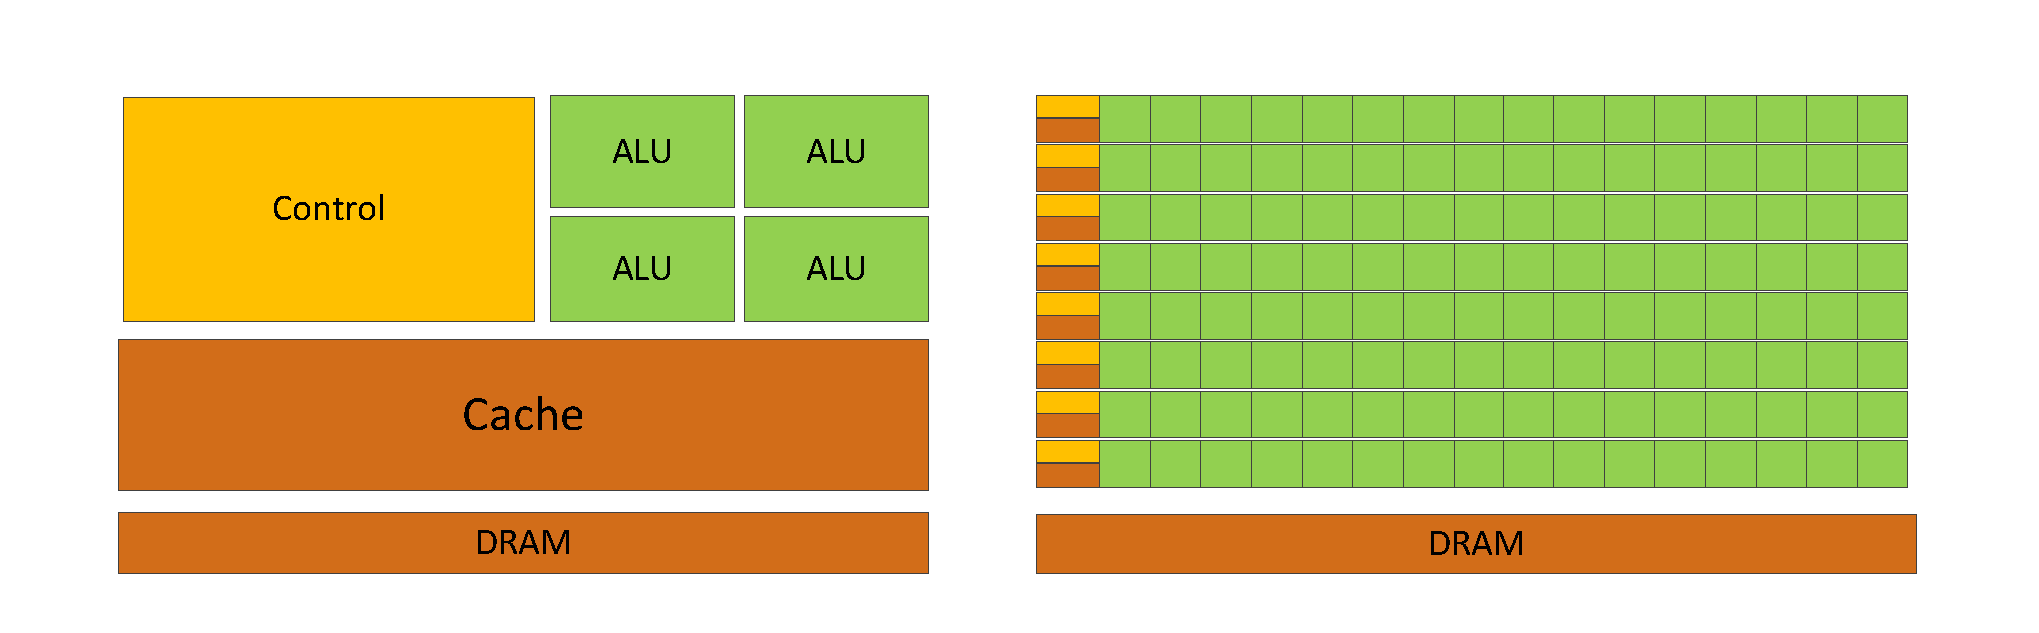
\includegraphics[width=1 \textwidth]{figures/GPU&CPU.pdf}}
\end{center}
\caption{{\footnotesize{GPU与CPU的区别}}}
\label{GCD}
\end{figure*}
\subsection{CPU与GPU区别}

图为 \ref{GCD} 为CPU和GPU的架构比较,可以看到,CPU和GPU的差异主要有两点,第一,GPU的ALU单元远远多于CPU。第二,GPU每个核心可用的逻辑控制单元和缓存相对CPU要少很多。CPU上大面积晶体管是逻辑控制单元和缓存单元,这是因为CPU的设计需要兼容多方面的应用,比如在桌面应用中就具有大量的分支控制操作和存储操作,而真正的数值计算操作却很少,所以CPU上具有大量的逻辑控制相关的实现,比如分支预测(Branch Prediction),乱序执行(OoO 来满足这些分支控制需求,同时增加缓存大小来加速存储过程,但是这样的设计也使得留给CPU上的计算单元的晶体管面积较少,浮点计算能力较差,现在CPU为了弥补其计算能力得不足,产商常常在同块芯片上集成多个CPU 核心,组成多核处理器,但是这样的设计并不能提高晶体管的利用率。

GPU最初被设计来进行图像渲染,图像渲染具有高度的并行性,而且大部分操作是浮点计算操作,逻辑控制较少,所以GPU在设计上采用简化控制单元,增加计算单元的设计思想,这使得GPU在进行大规模浮点运算的任务时大大优于CPU的执行速度。
\subsection{CPU+GPU异构计算模型}
通过上面的分析可以看到GPU适用于线程数目多,浮点计算密集和逻辑较简单的并行任务,而CPU更加适应与串行的分支较多,计算较少的任务。所以在实际中,常常把CPU和GPU结合起来,使用CPU和GPU两个部分协作共同完成并行计算任务,在这些并行任务中,CPU主要用于逻辑控制部分,而GPU 作为一种设备被CPU控制调用来做并行计算工作,这种协同工作模型被称为CPU+GPU 异构计算模型。
如图 \ref{GCY}所示为CPU+GPU异构计算结构示意图,GPU和CPU通过PCI总线进行连接。CPU调用GPU 执行一共需要以下步骤:

1.把输入数据从CPU主机内存拷贝到GPU的内存(全局内存)中。

2.把执行程序加载到GPU上然后执行。

3.GPU上的程序在执行过程中需要从主存中读取数据,为了加快线程访问内存的速度,数据将通过多级缓存进行缓存。

4.GPU上程序执行完毕,将结果写在GPU主存中,这时需要将结果重新拷贝回CPU主机端进行处理。
\begin{figure*}
\setlength{\belowcaptionskip}{-0.5cm}
\begin{center}
{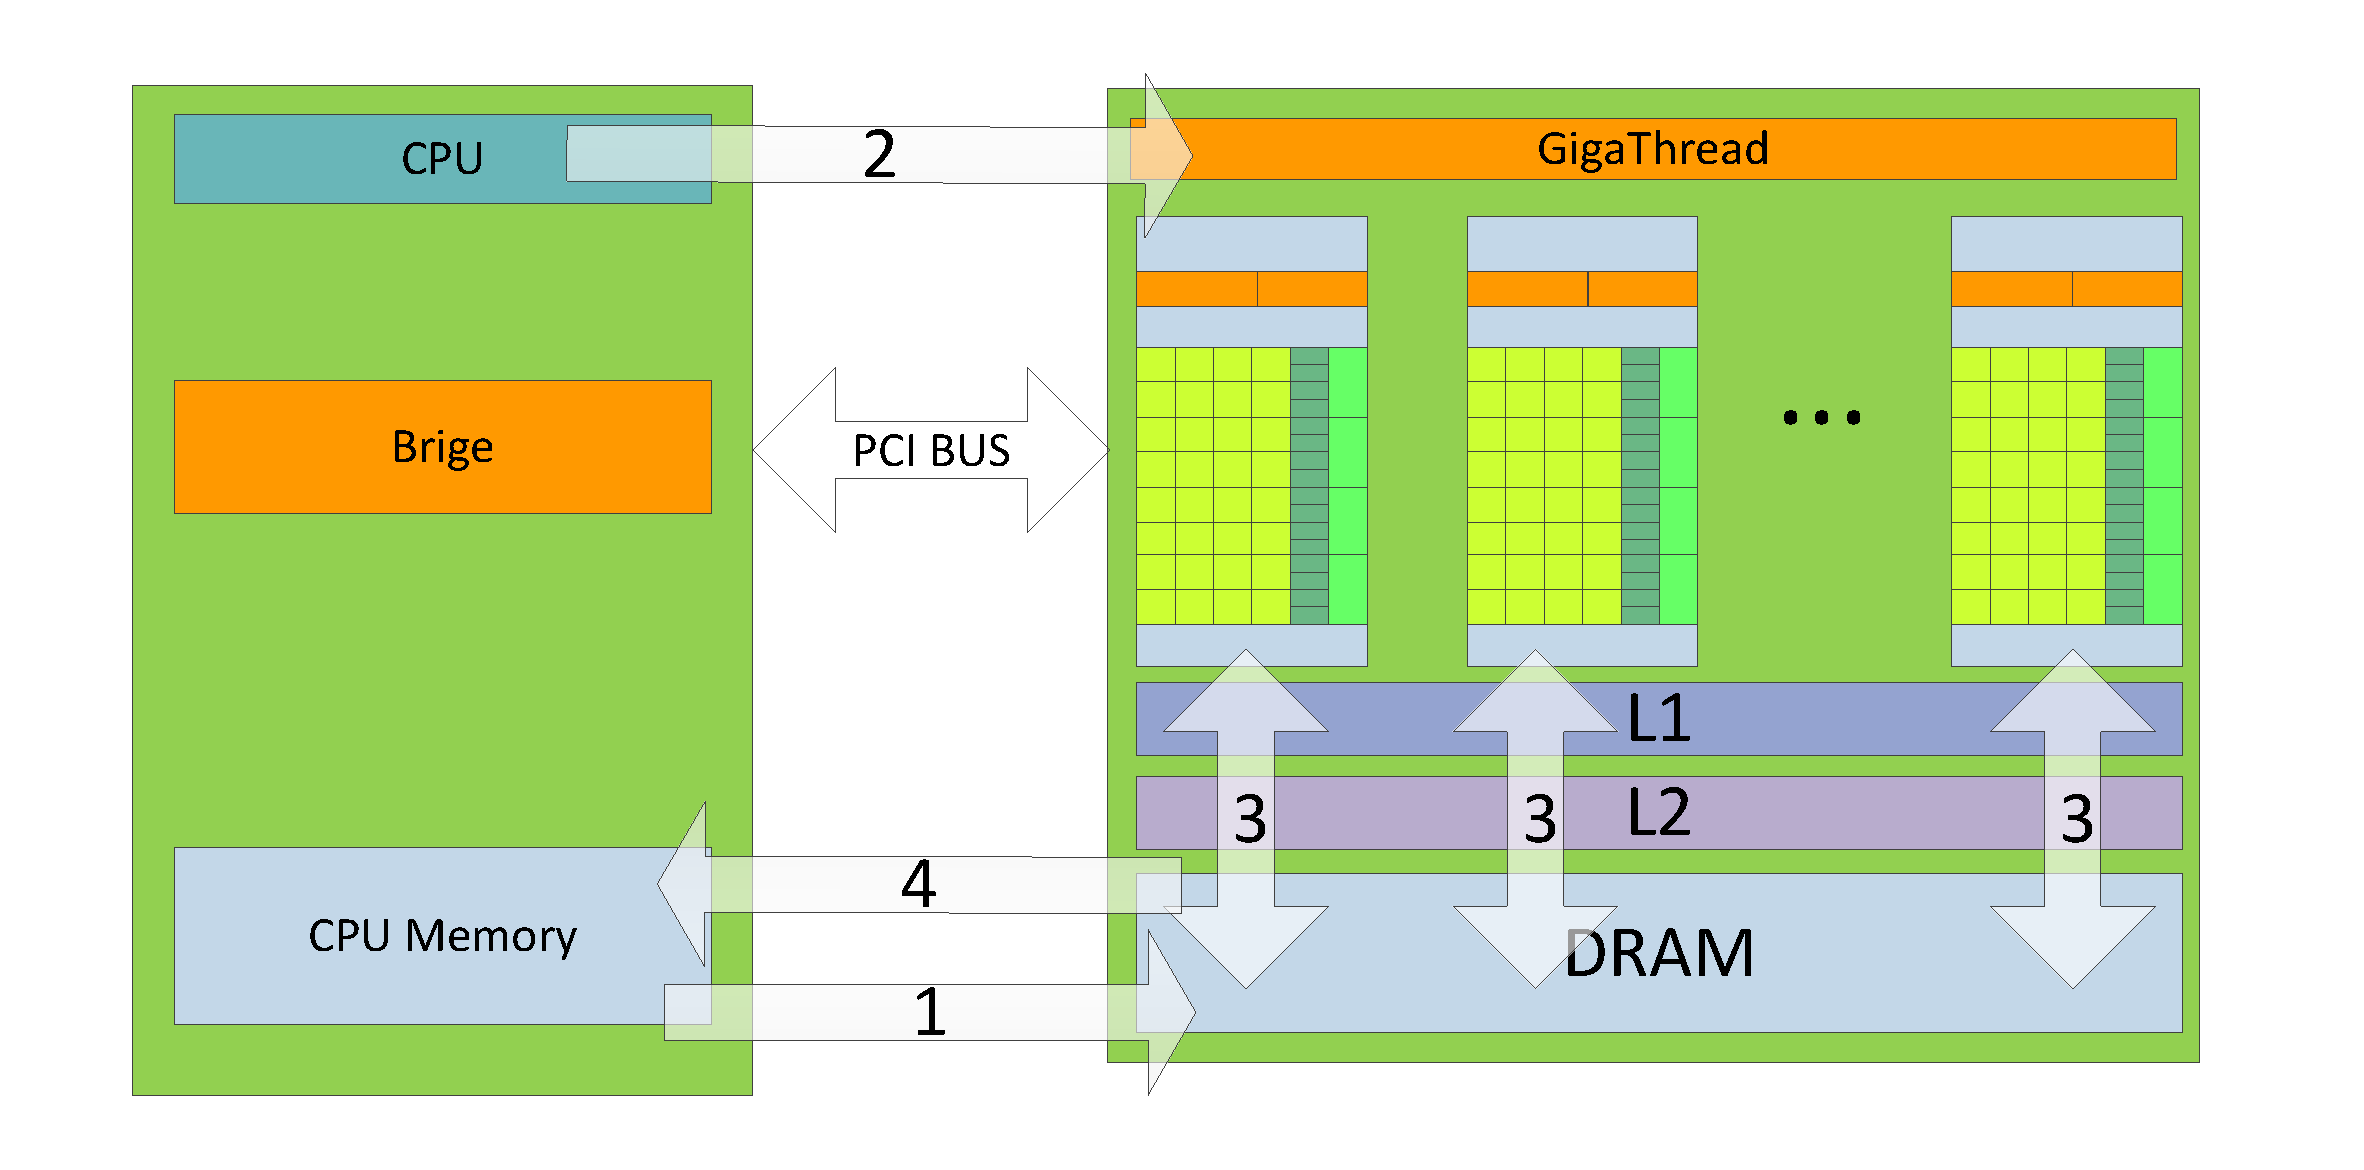
\includegraphics[width=1 \textwidth]{figures/yigou.pdf}}
\end{center}
\caption{{\footnotesize{GPU+CPU异构计算模型}}}
\label{GCY}
\end{figure*}
\section{GPU硬件架构}

虽然GPU相对于CPU在并行算法方面有很多优势,但是,由于GPU的出现是为了加速图形渲染问题,当想要使用GPU进行图形学之外的通用计算时,我们需要将问题转换为图形学问题,并且通过OpenGL或者DirectX等API来访问GPU,这对普通的开发人员提出了更高的要求,限制了GPU程序的设计自由度,使得GPU通用计算变得困难。2007年6月,NVIDIA推出CUDA (Compute Unified Device Architecture,统一计算设备架构)\citing{CUDA}。CUDA简化了在GPU上的通用计算流程,使用CUDA进行并行算法设计,不需要把问题转化为图形学问题去调用图形学API,同时,CUDA采用类似于C语言的语言结构进行开发,这使得开发人员可以很快地熟悉和使用CUDA进行开发。但是,要设计出快速高效的CUDA程序,开发人员需要掌握GPU架构上的相关知识,利用GPU的特殊架构来优化算法的设计。

我们以NVIDIA Kepler架构为例子来介绍GPU的硬件架构。图 \ref{KPA} 为Kepler的GPU架构模型细节,Kepler架构包含两个部分,流处理器阵列(core 部分)和存储系统(memory)部分,Kepler架构中的GPU上一共包含15个流多处理器(SM),所有流多处理器共享一个L2缓存。
\begin{figure*}
\setlength{\belowcaptionskip}{-0.5cm}
\begin{center}
{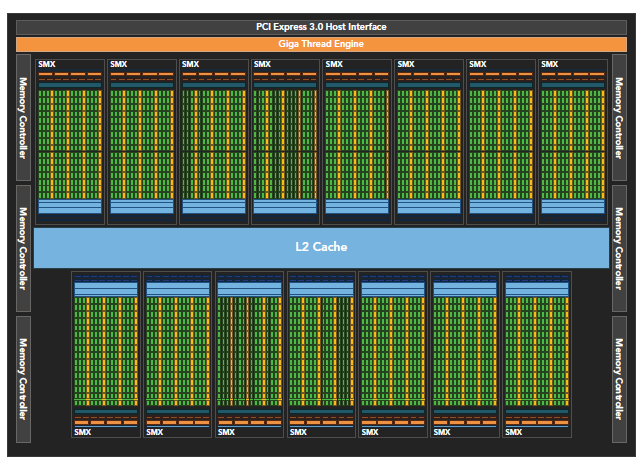
\includegraphics[width=1 \textwidth]{figures/arc.png}}
\end{center}
\caption{{\footnotesize{Kepler架构}}}
\label{KPA}
\end{figure*}
\subsection {流处理器}
我们看到GPU中主要组成部分是SM,一个SM(stream mutiprocessor)中含有大量的sp(stream processor),sp为GPU的计算核心,又称为流处理器,sp 是最基本的处办理单元,指令和任务最终都是sp上处理的,我们可以将在一个sp上执行的流看做一个独立的线程(thread),如果一个GPU中有更多的SM,一个SM中有更多的sp,那么就意味着这个GPU 在相同的时间内可以并行处理更多的任务。
\begin{figure*}
\setlength{\belowcaptionskip}{-0.5cm}
\begin{center}
{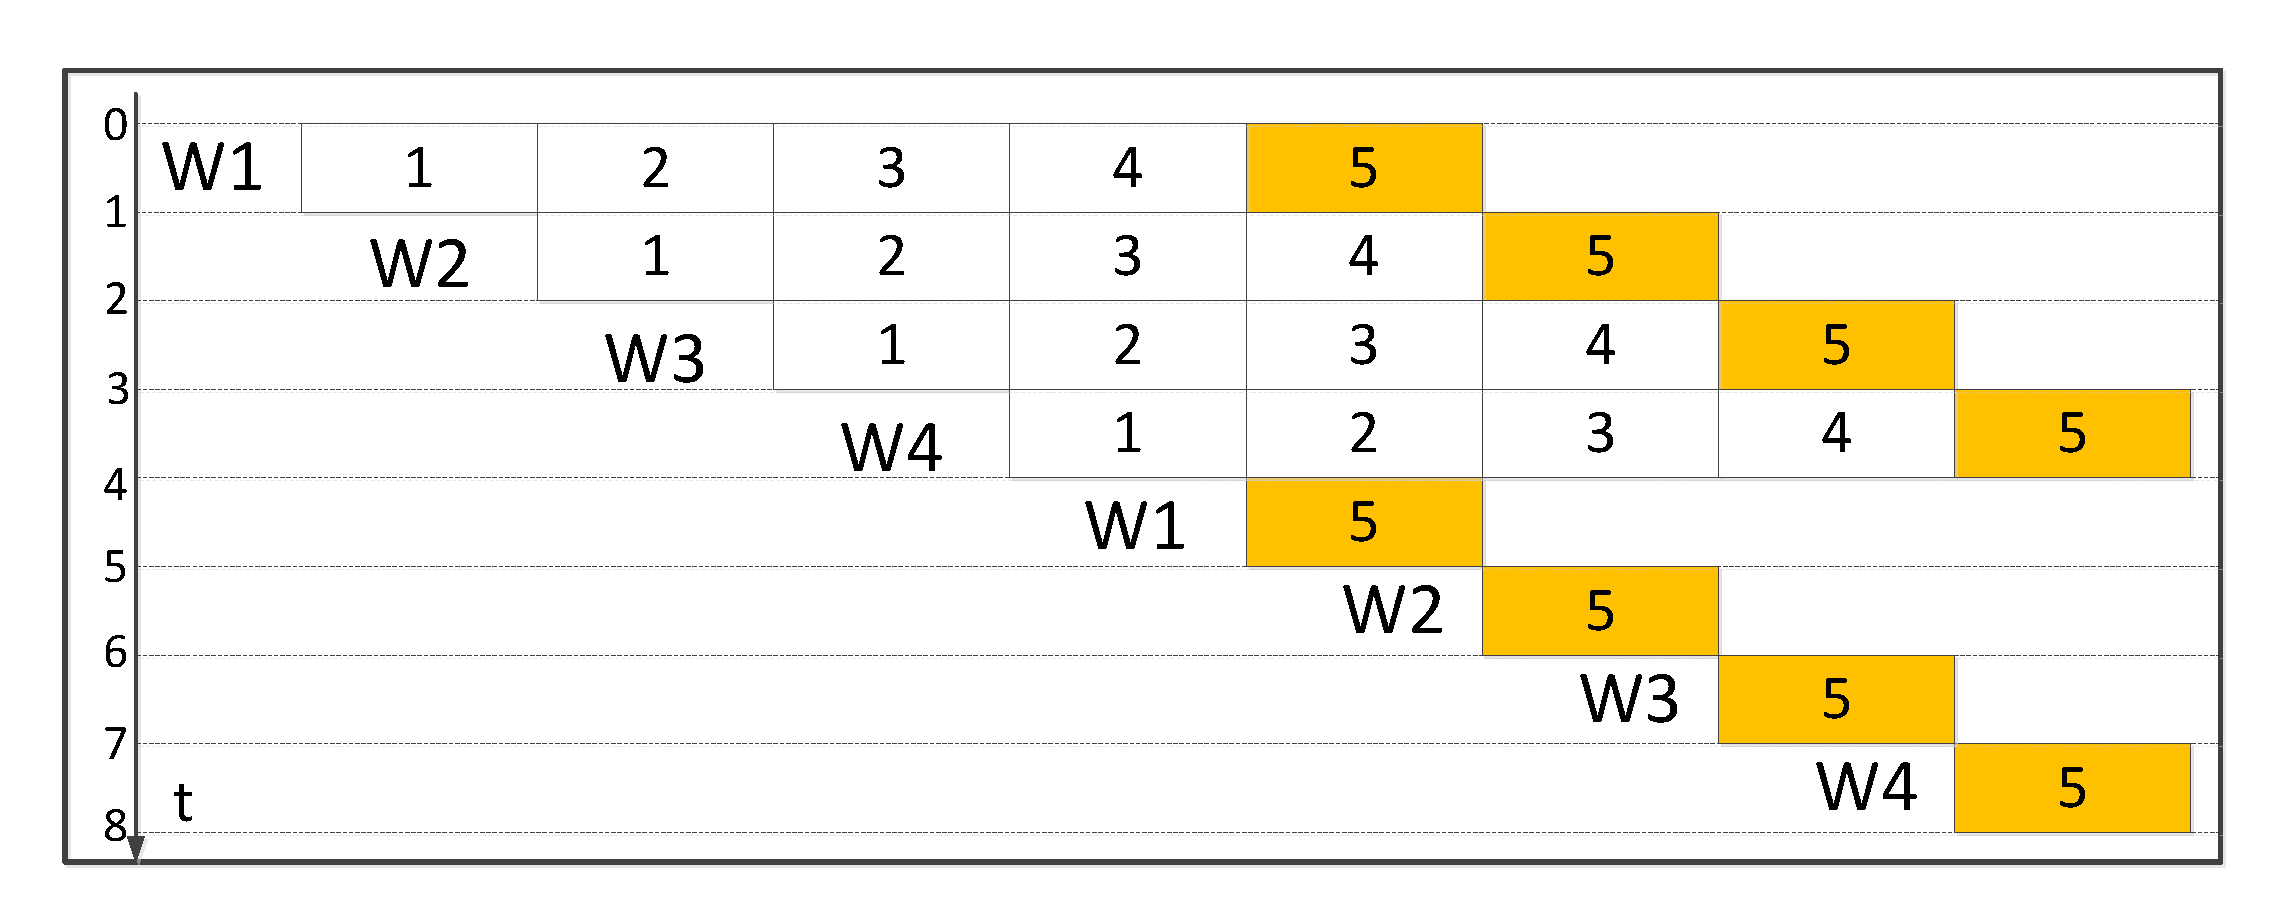
\includegraphics[width=1 \textwidth]{figures/warpsketch.pdf}}
\end{center}
\caption{{\footnotesize{warp切换示意图}}}
\label{wps}
\end{figure*}
\subsection{线程束(Wrap)}
warp是SM调度和执行的单位,一个SM中所有线程会被分成一个个warp组,通常一个warp组包含32个线程。同一个warp中的线程始终是同步的,这些线程都执行相同的指令,也就说同一个warp 中的线程必须等待所有线程都执行完了同一个指令后,才会去执行下一个指令,这样的设计虽然节省了硬件的控制单元的复杂程度,但是也限制了GPU 在处理分支时的并行粒度,如果同一个warp 中的线程出现分支,每个线程执行的分支条件不一样,为了保持同步,不进入分支的空闲sp 也必须等待进入分支的线程执行完毕后才能继续执行,这样使得sp 的利用率下降。

我们知道GPU 的浮点计算能力很强,但是在一些应用中常常需要进行内存的读写操作,这些访存操作需要大量的时间延迟,从而限制了GPU的浮点计算吞吐量,为了充分利用GPU 上大规模的sp,GPU采用warp 切换来隐藏这些延迟。同一个SM上可以存在多个warp的程序上下文,但是同一时间只有一部分warp被执行,下图 \ref{wps} 展示了warp上下文的切换过程,假设每个warp执行相同的代码,代码中需要先进行Load 操作,再进行计算操作,Load 操作需要等待4个时钟周期,而计算操作只需要使用一个时钟周期,W1-W4 表示4个不同的warp线程组,开始时W1先执行Load操作,而load 操作阻塞,这时warp调度器将W2调度到sp上进行执行,继续阻塞,直到第5个周期,W1的数据已经准备好了可以进行计算操作,当W1的计算操作结束后,继续切换计算W2,W3,W4。最终程序花费8个周期完成了对4个任务的计算,隐藏了12个周期的延迟,提高了sp的利用率。

\subsection{存储结构}
GPU中的每个SM中含有多种存储单元,包括寄存器,共享内存,常量内存,纹理内存。寄存器用来存储程序执行中的临时变量,同一个SM中的线程都能够访问共享内存,共享内存的访存速度大大高于主存的访存速度,所以在GPU并行代码设计时,我们常常先把频繁访问的数据提取到共享内存中,以减小延迟。另外,将中间结果存储在共享内存中,以减小对主存的访问,但是共享内存的大小是有限的,在Kepler架构中共享内存的大小为64KB。常量内存为只读内存,顾名思义他是用来缓存计算时需要的一些常量而专门设计的,常量内存大小为48KB。 纹理内存也是一种只读缓存,纹理内存是为图形学任务而设计的,在一些特殊的具有大量空间局部性的内存访问模式中能够提升性能并且减少内存流量。
\begin{figure*}
\setlength{\belowcaptionskip}{-0.5cm}
\begin{center}
{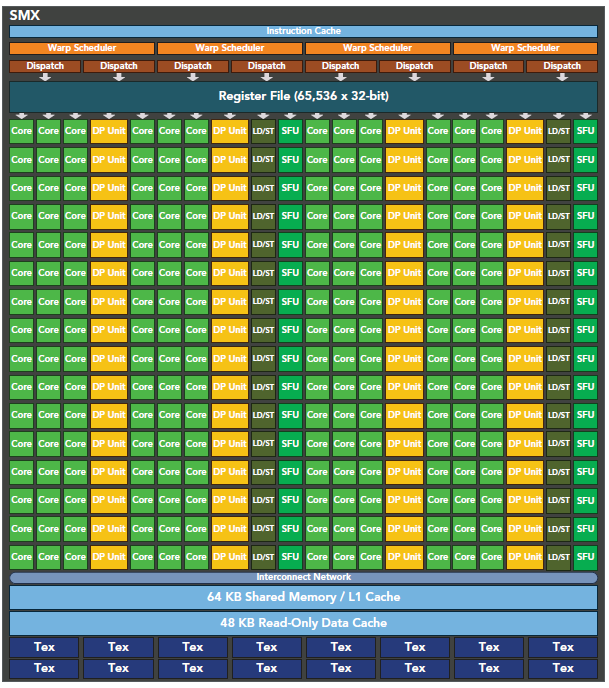
\includegraphics[width=1 \textwidth]{figures/smx.png}}
\end{center}
\caption{{\footnotesize{Kepler架构下的SM细节}}}
\label{sm}
\end{figure*}
\subsection{流多处理器细节}
通过上面对sp,warp和存储器的介绍,我们再介绍下Kepler架构下的SM细节。从图 \ref{sm} 中,可以看到,Kepler架构下的SMX中包含192个单精度的CUDA core,64个双精度的单元(DP unit)和32个SFU(Special Function Unit, 特殊函数单元),32个存储(load/store)单元,其中SFU用来执行超越函数、插值以及其他特殊运算。Kepler架构下的GPU的每个SM包含了4个warp调度器和8个指令发射器。 Kepler架构下的每个SM可以同时调度64个warp共计2048个thread,而Kepler架构中一共有15个SM,也就是说,同一时刻最大可以支持30720个线程在GPU上调度执行,所以GPU的并行能力相当强大。

\subsection{执行模型}
GPU的执行模型被称为SIMT(Single Instruction ,Mutiple Thread),SIMT是对SIMD的一种改进\citing{CUDAR}。在CPU的SIMD中,向量宽带是受限的,在Intel 的SSE指令集中,假设一条SSE的指令宽带为128bit,那么它一次可以处理4个单精度浮点数,如果要用SSE指令处理一个单精度浮点数组,必须将数组打包成4个一组,然后才能把这些组交给CPU进行计算。但是在CUDA的模型中,我们为相同的指令产生不同的线程,这些线程的数量可以自由设置。在Kepler架构中,同一时刻GPU上可以调度执行30720个线程,这比CPU的SIMD的并行粒度高很多。

\section{CUDA编程模式}
CUDA是一种异构计算模型,CUDA程序在CPU和GPU上交互执行,CUDA的程序可以分为主机部分和设备部分,设备代码在一个或者多个GPU上执行,主机部分的代码在主机上执行,负载调度GPU上的设备代码执行过程。图 \ref{ktz} 展示了CUDA 异步执行流程,CPU通过调用kernel 函数的方式控制GPU 执行并行程序。
\begin{figure*}
\setlength{\belowcaptionskip}{-0.5cm}
\begin{center}
{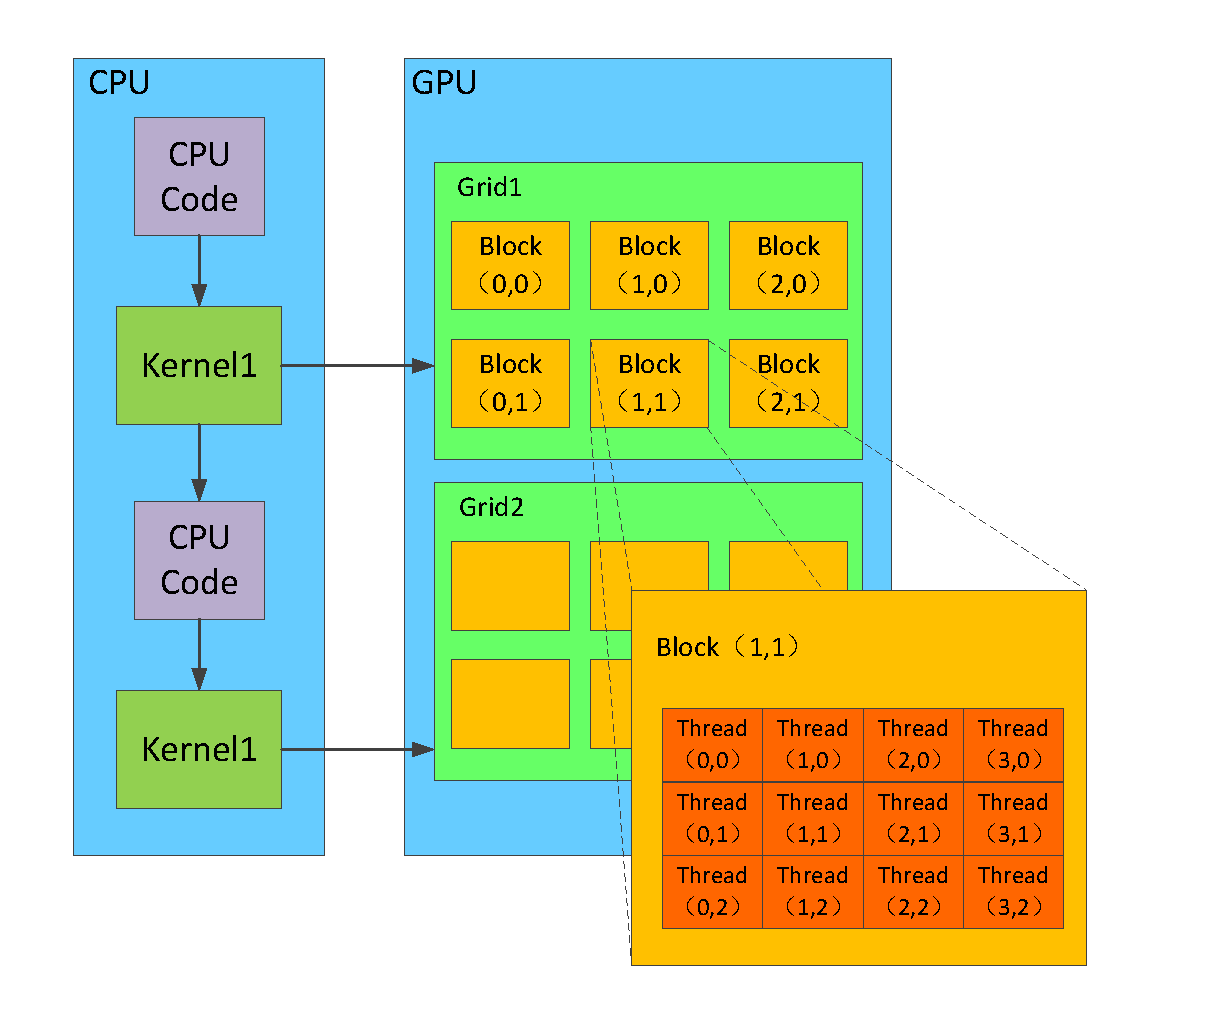
\includegraphics[width=1 \textwidth]{figures/block.pdf}}
\end{center}
\caption{{\footnotesize{CUDA异构执行流程和线程组织}}}
\label{ktz}
\end{figure*}
\subsection{CUDA软件线程组织}

一个CUDA程序包含大量并行执行的线程,在软件层面上,我将多个线程组成一个block,同一个block中的线程又被分成不同的warp组,一个block中的线程只能在同一个SM中执行,同一个block中的线程可以通过调用同步函数(\_\_syncthreads())进行同步,同一个blcok中的线程可以共同访存shared\_memory,通过shared\_memory实习通信。一个kernel函数可以在软件层面上产生大量的线程,这些线程被组织成一个一个的block,如果SM足够,这些block中的线程将被加载到SM 上调度执行,如果SM不足,block需要排队等待其他block完成执行。多个block组成一个Grid,block的维度可以是1-3维,图 \ref{ktz}展示了一个二维的block组织,每个block有自己的二维标号,同样每个block内部的线程也可以被组织成1-3维,图 \ref{ktz}展示了一个block内部的thread二维标号。

\subsection{kernel函数}
kernel函数是GPU上每个线程执行的函数,kernel函数在主机端调用,在GPU端执行,在调用kernel函数时需要为kernel函数设置一些参数,包括Grid维度大小和block维度大小。在kernel函数中使用blockIDx.x,blockIDx.y,blockIDx.z三个标号来访问当前block在Grid中的三维坐标,使用threadIDx.x,threadIDx.y,threadIDx.z三个标号来访问当前线程在block中的三维坐标的。kernel函数中使用blockDim.x,blockDim.y,blockDim.z分别表示block的三个维度的宽度。

\subsection{CUDA线程同步}
2.2.2介绍过同一个warp中的32个线程的执行是天然同步的,但是如果程序中存在更多的线程需求的话,我们就不能仅仅依赖于warp的性质进行同步,CUDA支持同一个block中的所有线程进行同步,通过调用同步函数\_\_syncthread(), 一个block 中的线程可以实现同步,它表示block中所有的thread都要同步到这个点(\_\_syncthread()执行处)才能继续执行,这种同步操作相当与CPU上多线程的barrier(屏障)操作。GPU上的线程同步的另一个问题是线程的写操作的同步问题,多个线程同时写相同地址的数据不是线程安全的。CUDA提供了一系列的原子操作来对多个线程间的共享数据的读写进行互斥保护,比如atomicAdd函数,他对目标地址的值进行原子加法操作,保证每次只有一个线程对数据进行加法操作。

\subsection{CUDA流并行}
CUDA程序通过流来管理并发,CUDA流代表一系列的GPU操作组成的队列,这些队列内部的操作按照顺序在GPU上执行,当我们调用kernel函数或者调用CUDA内部函数(cudamemcpy(),cudasyncthread()等)时,就是把一系列的GPU操作加到一个CUDA流队列中,这个流队列的操作会在GPU上按照加入的顺序执行。GPU上可以同时存在多个流队列,不同流之间的操作是无关的,流之间可以相互切换以充分利用GPU上的计算资源,虽然同一个流中的操作必须顺序执行,但是不同流之间的操作顺序是乱序的,而且还有可能是同时并行执行的,所以流并行也是GPU上的一个并行层次,我们可以把它视为任务上的并行,每个流代表了不同的任务,不同任务间的操作可以不断切换来隐藏延迟,从而提高了GPU的SM利用率,增大了并行粒度。同时,任务上的流并行,对编程人员来说是比较容易理解的,给GPU的并行代码设计带来了方便,我们可以为相似的任务设计相同的代码,通过流并行提高并行粒度,减小了设计难度。

我们观察下面图\ref{flow}中简单的流并行例子,来分析流并行的优势,图\ref{flow}中的Copy Engine表示GPU上的内存拷贝单元,负责和CPU端进行数据传输,Kernel Engine表示GPU上的kernel执行单元,负责kerenl的调度执行。在图 \ref{flow}(a) 中一个有两个流,两个流的操作相同,假设图中的每一个操作的执行时间相同,那么如果两个流串行执行,则总共需要6个时间单位,但是如果两个流相互切换,当Copy Engine在进行复制操作的同时,stream0的kernelA在Kernel Engine上执行,当stream0的kernelA执行完毕后,stream1的kernelA也已经准备好可以执行了,这样Copy Engine的数据传输带宽和GPU的计算带宽都得到充分利用,一共只需要4个时间单位,就可以完成两个流的操作。图 \ref{flow}(b) 中,假设两个流的复制操作比较少,而kernel需要的计算时间较长,这个时候由于两个流的kernel都会很快准备好发射,如果SM资源足够,两个kernel将同时在GPU上调度执行,如图\ref{flow}(b)中的红色部分表示重叠执行的时间,可以看到这种情况下多个流的并行可以大大节省运算时间,充分利用SM资源。
\begin{figure*}
\setlength{\belowcaptionskip}{-0.5cm}
\begin{center}
{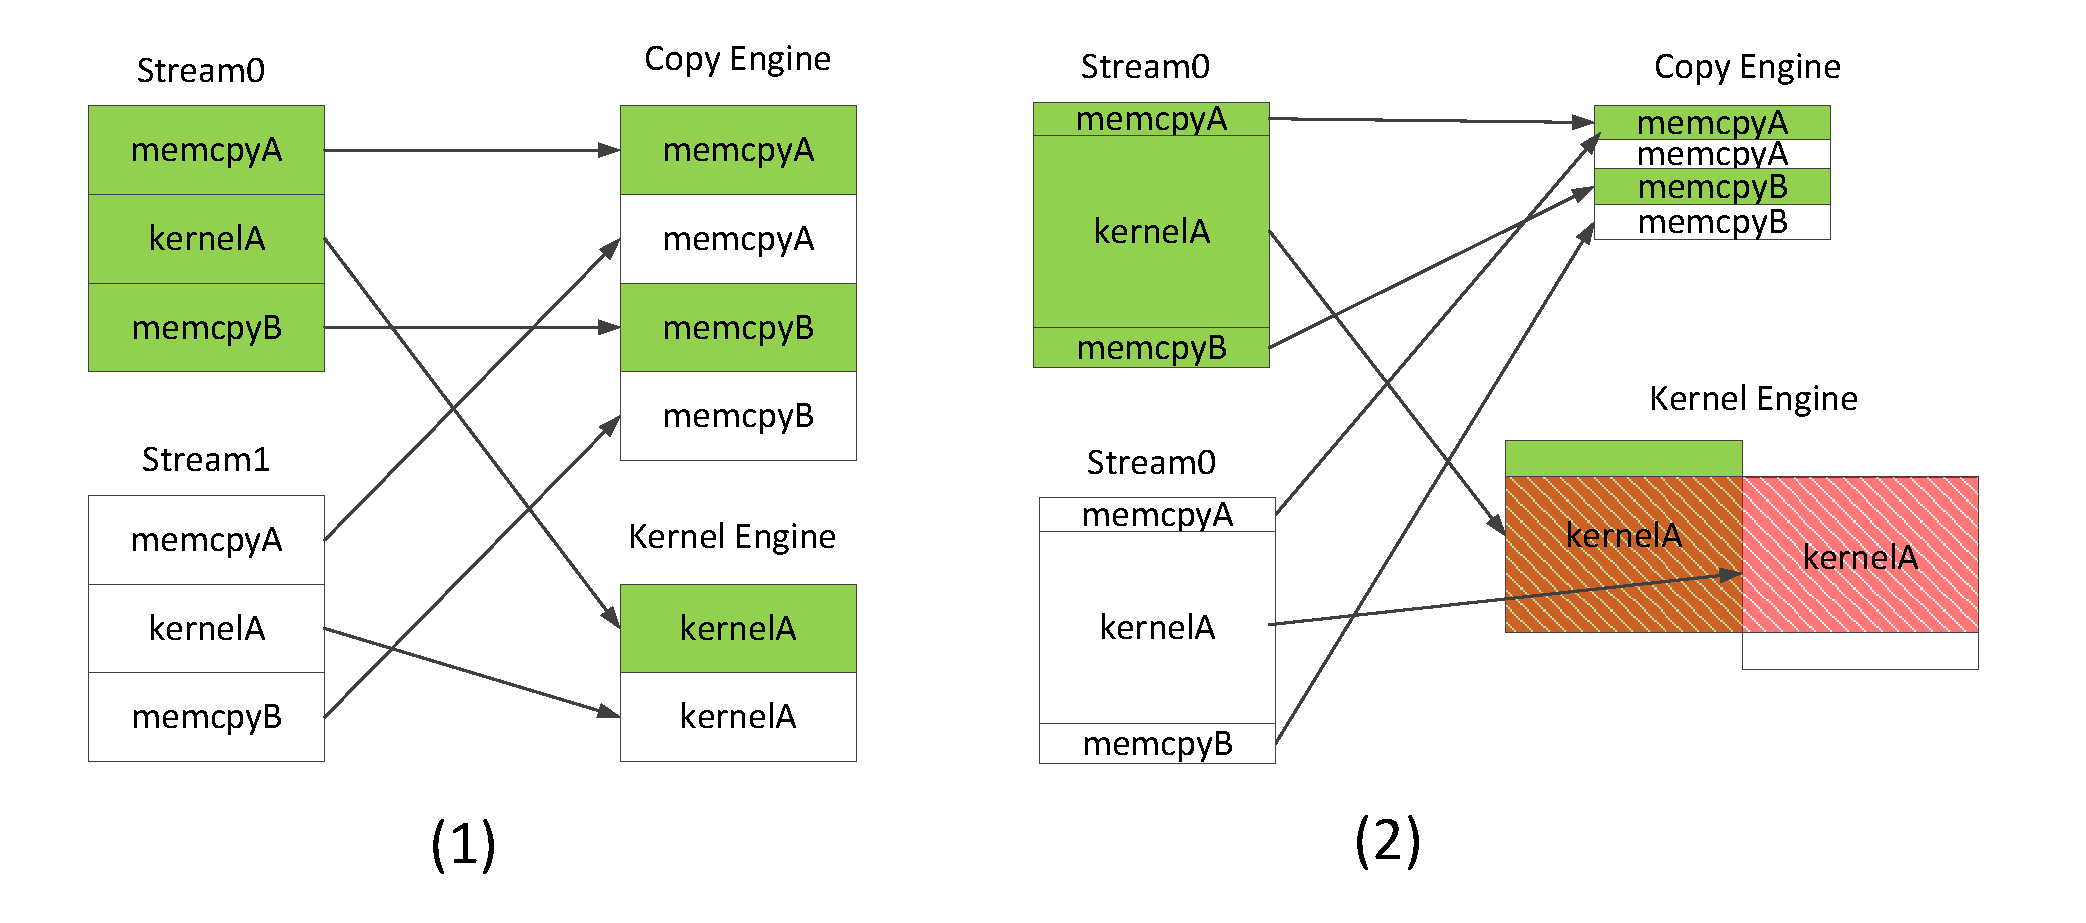
\includegraphics[width=1 \textwidth]{figures/flow.pdf}}
\end{center}
\caption{{\footnotesize{流并行示意图}}}
\label{flow}
\end{figure*}
\subsection{本章总结}
本章简略介绍了GPU的体系架构和CUDA编程框架,说明了GPU的的强大计算能力和一些GPU程序设计上需要注意的问题,为后面的3,4章介绍做铺垫。

% !Mode:: "TeX:UTF-8"
\chapter{SDN网络下的并行路由优化算法设计}
\section{引言}
对大规模业务的路由优化问题可以建模成一个多商品流问题,将网络路由业务作为输入,寻找最优的路由路径来最优化效用函数,效用函数通常设置为对网络拥塞程度的评价水平,比如,最常用的效用函数是最小化最大链路利用率(MLU),简单地被定义为利用率最高的那条链路的链路利用率[],另外一些把所有链路的链路利用率的和作为效用函数([],[])。这些效用函数的逻辑是:(1)低链路利用率意味着低的网络延迟。(2)维持低的链路利用率意味着预留更多的空间给其他将来到达的业务。但是大量基于实际拓扑的实验表明链路利用率效用函数,特别是链路利用率,在网络利用率没有达到拥塞程度的时候,不是对网络优化的较好评价函数[]。在这个实验中,当链路利用率低于0.9的时候会造成不可忽略的网络性能中断,反之,在网络发生大量拥塞的情况下MLU只去优化最大的链路利用率,而不能给出一个可行(满足容量约束)的解。所以作为替代,文章在链路容量约束的情况下来优化路由总代价。我们假设已经知道短时间内到达的一批业务,控制器需要计算出满足链路容量约束的路径,并且最优化链路路由总代价。为了使得加入网络的业务尽量多,我们设定被阻塞的业务代价为一个较大值。本文中考虑的优化问题是一个NP-hard 问题,因为他等价于一般的带整数约束的商品流问题[]。

本章主要设计两种路由优化算法,第一种是基于备选路径选择的路由优化算法,采用遗传算法来优化目标函数,并且设计了遗传算法的并行版本,获得几十倍的加速比,第二种是基于拉格朗日松弛的优化算法,算法把链路容量约束松弛到目标函数,并把路由优化问题分解成一堆路由路径计算问题,从而采用GPU进行并行计算。
\section{网络模型和问题建模}
\subsection{网络模型}

本文将SDN网络建模成无向图 $G(V, E)$,$V$表示所有的点集合, $E$是所有边的集合, $n = |V|$ 和 $m = |L|$ 分别表示点数和边数。对每一条边$(i,j)\in E$, $w_{ij}$ 表示此边 $(i,j)$上的权重(传输一单位的流量需要的代价),不失一般性,我们假设每条链路上的$w_{ij}$是整数,对每一条边 $(i,j)$, $c_{ij}$表示此边上的容量,假设$D$表示需要被路由的业务需求集合,业务$d \in D$ 是一个元组 $(s_d, t_d, bw_d)$,其中, $s_d$表示业务的源节点,$t_d$表示业务的目的节点,$bw_d$表示业务d需要的流量带宽。业务量工程问题将网络业务需求和网络拓扑作为输入,计算出每条业务的路由路径以使得效用函数代价最小化,在SDN 网络中,业务的路径在中心控制器上计算出来,为了满足用户业务的QoS 要求,本文假设链路利用率不能超过一个固定阈值 $\theta$,因此,一些业务会因为链路上容量不足而被阻塞,本文用 $\hat{D}$来表示这些被阻塞的业务集合。
\subsection{问题建模}
本小节,我们把路由优化问题建模成一个混合整数规划模型(MILP),本文采用新的效用函数,如下:
\begin{equation}\label{Obj1}
f(\mathbf{d})=\begin{cases}
\sum\limits_{d \in D} c(p_d) & \text{if available bandwidth is enough}\\
\sum\limits_{d \in \hat{D}} bw_{d}& \text{otherwise
}
\end{cases}
\end{equation}
其中$p_d$是计算出来的对应于业务$d$的路径,$c(p_d)$ ($c(p_d) = \sum_{(i,j)\in p_d} w_{ij}$) 表示的是此路径$p_d$ 的代价。因为不知道带宽是否足够容纳所有业务,(1)并不是衡量所有情况,为了衡量所有情况,我们对$G(V, E)$构建辅助图$G_a(V_a, E_a)$,初始时,让$G_a(V_a, E_a) = G(V, E)$,然后,对每个点$v \in V$ 和 $u \in V$,在$G_a(V_a, E_a)$ 中添加一条链路 $(v, u)$,并且设置链路 $(u,v)$ 的容量和代价分别为 $\infty$和 $nM$ ,其中 $M$是 $G(V, E)$ 中最大的链路代价,这样,$G_a(V_a, E_a)$就有足够的容量来容纳业务需求,如果某条业务被路由到$G_a(V_a, E_a)$中,那么就表示这条业务被阻塞了,加入了辅助图$G_a(V_a, E_a)$后,路由优化的效用函数可以表示为:
\begin{equation}\label{Obj2}
z^* = minimize~f(\mathbf{d})=
\sum\limits_{d \in D} c(p_d)=  \sum\limits_{d \in D}\sum\limits_{e \in p_d} w_e
\end{equation}
在本文的路由优化问题中,每个业务只能够路由到一条路径上,这与SDN网络的实际情况相符,以下整数约束能够保证每个业务只走一条路径
\begin{equation}\label{FlowConv}
\begin{split}
\sum\limits_{(i,j) \in E_a} x_{ij}^d - \sum\limits_{(j,i) \in E_a} x_{ji}^d
=\begin{cases}
1 & \text{if $i = s_d$}\\
-1 & \text{if $i = t_d$} \\
0 &{ohterwise}
\end{cases}
\\~~~~~~~~\forall i\in V_a, \forall d\in D
\end{split}
\end{equation}
其中 $x_{ij}^d$是一个0,1整数变量, $x_{ij}^d=1$表示业务$d$路由经过链路$(i,j)$,为了避免链路拥塞,路由路径需要满足以下的链路容量约束:
\begin{equation}\label{Capcon}
\sum\limits_{d \in D}\sum\limits_{(i,j) \in E_a} x_{ij}^d \cdot bw_d \le \theta\cdot c_{ij} ~~\forall (i,j)\in E_a
\end{equation}
在这个模型中,变量的数量随着业务量大小和网络规模大小呈指数增长,所以这个MILP模型在大规模情况下很难求解。
\section{基于遗传算法的路由优化算法}
遗传算法是一种模拟自然进化过程搜索问题最优解的启发式算法,遗传算法模仿达尔文进化论和自然选择过程来评价挑选最优解集合,从而找寻较优化的解,遗传算法从一个代表问题的可行解的种群出发,一个种群中不同个体代表了不同的解,每个个体实际上是一个染色体,染色体携带表达当前解的信息编码,初代种群产生后,对每个染色体个体进行评价,按照适者生存,优胜劣汰的原则,使得较优的个体更有可能把自己的遗传信息传递给下一代,从而得到更优化的后代,算法过程中,对一部分基因进行变异,好的变异能够提高解的质量,增加算法的搜索空间,避免算法收敛于局部最优解。遗传算法的步骤流程图如下 \ref{IterNum} 所示:
\begin{figure}
\setlength{\belowcaptionskip}{-0.5cm}
  \begin{center}
    {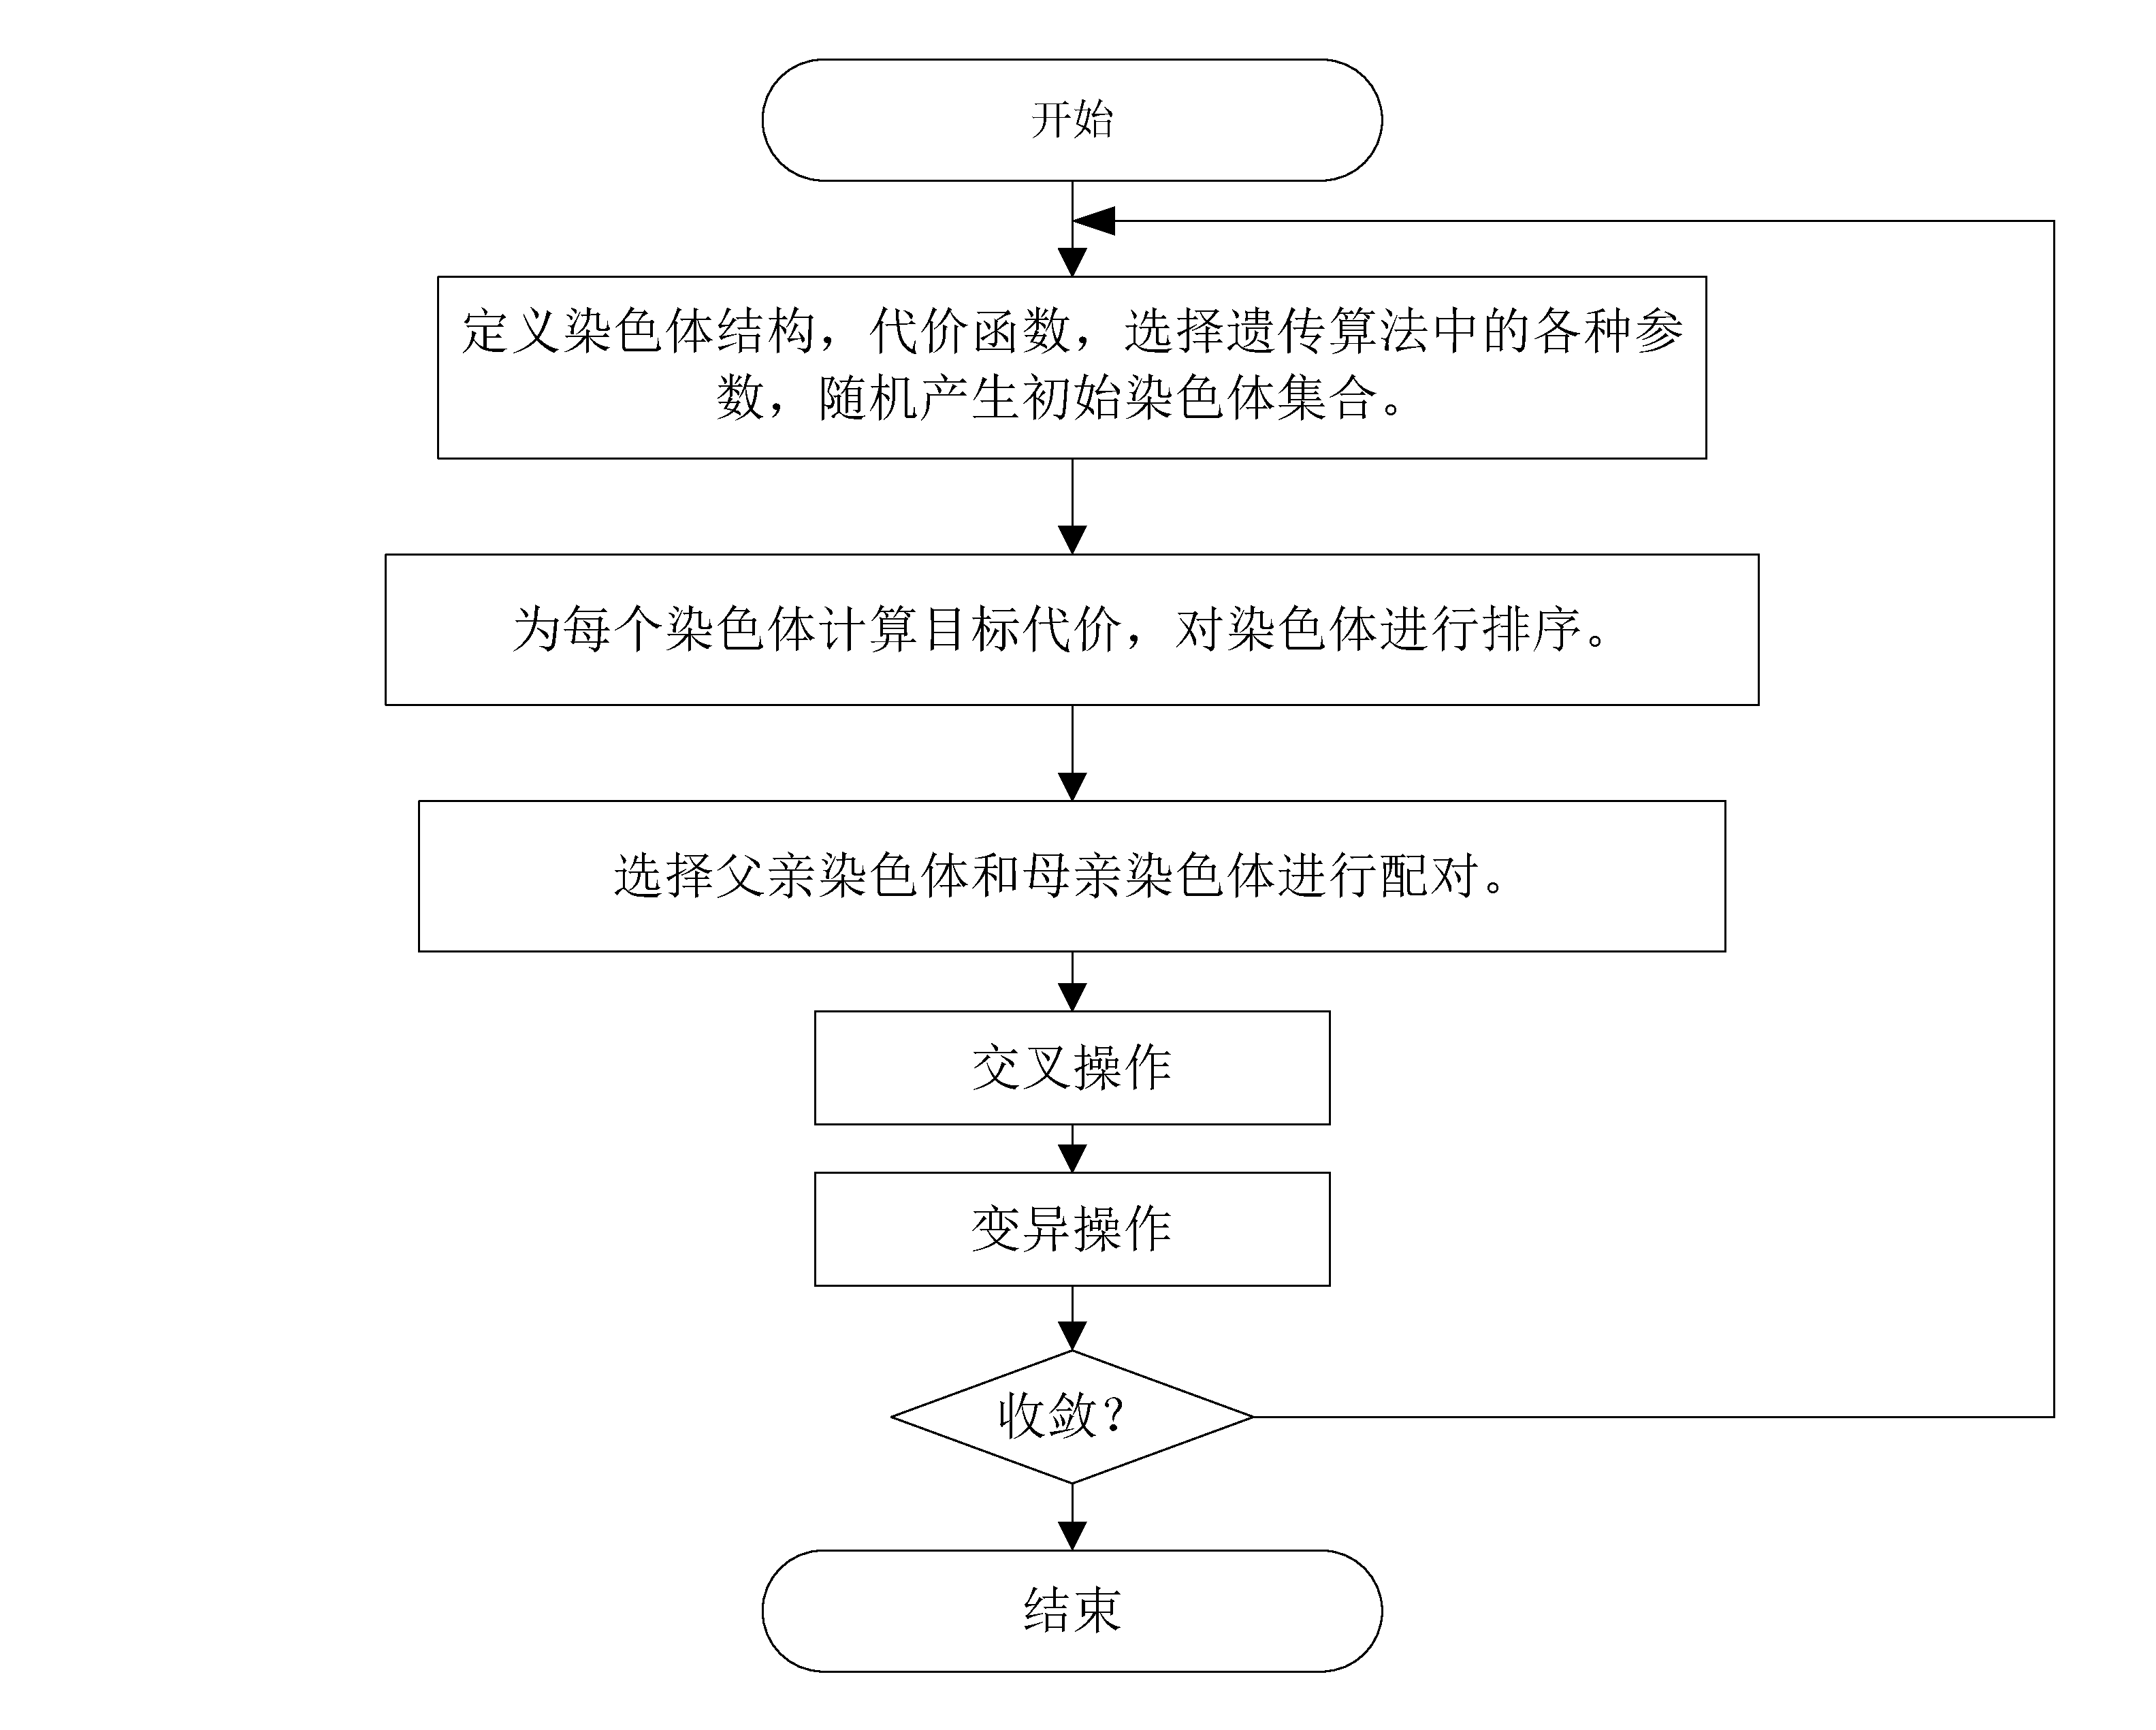
\includegraphics[width=0.45 \textwidth]{figures/GAprocess.pdf}}
    \end{center}
  \caption{{\footnotesize{GA算法流程图}}}
  \label{IterNum}
\end{figure}
\subsection{遗传算法设计}
\subsubsection{定义染色体结构}

由前面的讨论可以知道,路由优化问题求解过程是寻找最优的业务路径集合,使得效用函数最小化,在论文[]中作者(效用函数是常见的最小化最大链路利用率)提出了一种路由优化算法,在文章中,为每一个业务$d \in D$,产生$K$ 条不同的备选路径作为备选路径集合$P_i={p^1_d,p^2_d,p^3_d...p^K_d}$, 通过遗传算法过程来确定每个业务选择哪一条备选路径,从而找到最优解,本文采用相同的思想来求解路由优化问题,假设业务数量为$|D|$,初始染色体集合大小为$POP$对于第$j$ ($j in [1:POP]$)号染色体一个染色体$C_j$ 是一个$|D|$维数组,$C^i_j=k,k \in[1:K]$ 表示在第$j$号染色体中,业务$i$ 选择了第$k$条备选路径,$C^i_j=-1$表示业务$i$不加入网络中(在辅助图上路由),不占用链路资源,$|p^i_d|$表示业务$d$的第$i$ 条备选路的路径代价,$rp^i_d$ 表示路径$p^i_d$ 上的最小可用容量,$rp^i_d=min(r_e|e \in p^i_d)$,其中$e \in p^i_d$ 表示路径$p^i_d$上的边,$r_e$ 表示此边$e$ 上的剩余容量。
\subsubsection{初始可行解生成}
可行解表示满足容量约束的解,为了使得遗传算法有效,初始解的质量很重要,产生的初始解要尽量好,要有更多的业务要能加入网络中,而且保证业务的路径代价较小,文章中采用一种简单的贪心算法产生出初始可行解,算法过程如下 \ref{alg:Framwork} 所示:
\begin{algorithm}[htb]
\caption{初始可行解产生}
\label{alg:Framwork}
\begin{algorithmic}[1]
\Require{$G(v,E)$:网络拓扑;$P$:备选路径集合;$C$;未初始化的染色体集合;}
\Ensure{$C$:可行染色体集合;}
\For{each $c_j \in C$}
\For{each $c^d_j \in c_j$ }
\State {$c^d_j \leftarrow -1$}
\EndFor
\EndFor
\For{each $c_j \in C$}
\For{each $c^d_j \in c_j$ }
\State {$c^d_j\leftarrow k^d_j$,其中$k^d_j$为1到K之间的随机值,随机选择一条备选路}
\EndFor
\State {对染色体中的的每个业务需求按照值$\frac{bw_d}{\sqrt{|p^{k^d_j}_d|}}$}进行降序排序。
\For{each $c^d_j \in c_j$ }
\If{$rp^{k^d_j}_d>=bw_d$}
\State 加入路径$p^{k^d_j}_d$到网络,更新网络链路容量。
\Else
\State {$c^d_j \leftarrow -1$}
\EndIf
\EndFor
\EndFor
\end{algorithmic}
\end{algorithm}

对某一个染色体,算法随机为每个业务生成所选择的备选路径编号,但是这样选择出来的路径集合有可能会超过网络链路的容量限制,从而使得解变得不可行,要得到可行解,必须从染色体中剔除一部分业务,使得他们阻塞,为了得到比较优秀的初始可行解,本文提出一种启发式过程来确定能加入的业务,以及必须剔除的业务,一方面,要使得目标函数变小,那些流量需求较大的业务应该优先被加入到网络中,但是如果大流量的业务的路由代价很大,经过了一条很长的路径,就会大量的浪费网络中的链路容量资源,所以算法过程对当前染色体$j$中的业务和其路径按照$\frac{bw_d}{\sqrt{|p^{k^d_j}_d|}}$ 的值进行排序,其中${bw_d}$ 代表当前业务$d$所需要的流量大小,$|p^{k^d_j}_d|$代表当前染色体$j$ 所选择的$p^j_d$ 中的第${k^d_j}$ 条路径的代价大小。这样算法优先加入$\frac{bw_d}{\sqrt{|p^{k^d_j}_d|}}$值较大的业务,观察目标函数,目标函数是优化路由代价最小,而$\frac{bw_d}{\sqrt{|p^{k^d_j}_d|}}$较大意味着较大的流量经过较小代价的链路进行路由,这种路由是很理想的,尽量节省网络的链路使用资源的同时,又减小了总体目标函数,所以这个比例值是对业务路由个体优劣程度的较好评价,于是文章采用这个比例值来确定路径加入网络的优先级(后面第节也会应用类似的思想来调整路由),每次按照比例值排序的结果将遗传染色体所选择的路径$p^{k^d_j}_d$ 尝试加入到网络中,如果$rp^{k^d_j}_d>=bw_d$,表示路径经过的链路有足够的容量来容纳这一个业务,所以加入业务到网络中,并且更新网络的链路容量大小,反之,如果$rp^{k^d_j}_d<bw_d$,这个业务选择这一条路径会超过网络链路的容量限制,于是这条业务被阻塞,染色体中的相应基因位置被设置为-1。大量重复以上可行解的产生过程,则可以得到一个较好的初始染色体集合$C$。
\subsubsection{评价与交叉}
评价过程对本轮产生的染色体,计算其相应的目标效用函数值,并且对染色体按照效用函数目标进行降序排序,由于算法过程随机交叉,可能会产生不可行的染色体解(链路容量超限),把这样的染色体评价为一个个很大的代价,从而在选优时被排除掉,目标值排在最前面的前$\alpha$ 个染色体为最优集合$A$,这个集合中的染色体为精英染色体,精英染色体将直接保留到下一轮迭代,此后的$\beta$个染色体为较优染色体集合$B$,较优染色体集合中的染色体不会直接保留到下一轮,但是他们有繁殖的权利,可以和精英染色体一样产生后代,遗传自己的选路信息,排在最后面的$\gamma$ 个染色体,组成劣等染色体集合$G$,由于其目标值一般较大,其选路策略不可取,算法直接扔掉这一部分劣等染色体,而且不让劣等染色体进行繁殖。

交叉过程从精英染色体集合中$A$中随机选取一个染色体$c_i \in A$作为父亲,从精英染色体集合和较优染色体集合的并集$A \cup B$ 中随机选取一个染色体$c_j \in A \cup B$ 作为母亲,将$c_i$ 和$c_j$进行均匀交叉得到新的染色体$s$,均匀交叉过程示意如下所示,均匀交叉的过程是,对$s$的每一个基因点位以$\%50$的几率选择继承父亲或者母亲的相应点位的路径选择。重复以上过程$\beta+\gamma$ 次,从而产生$\beta+\gamma$ 个新的子染色体来替换当前染色体集合评价函数排在后$\beta+\gamma$个的染色体,因此得到新的染色体集合$C$。
\subsubsection{变异与迭代终止}
变异过程采用随机变异,随机在已经交叉后的集合$C$中选取$M \in [0:POP]$条染色体,对某一选定的染色体$c_j \in C$, 随机选取$m$个业务基因点位,进行变异,将当前已经选择的路径编号随机改变为备选路集合中的另外一个值,由于变异过程是为了提高算法的的搜索空间,避免算法陷入局部最优解,但是实际实验过程中发现如果$M$和$m$ 值设置较大,可能使得算法收敛较慢,因为大量的变异可能会导致较优秀的可行解变成不可行,因此会丢掉这些优秀的解,因此实验中$M$ 和$m$ 的值设置得较小,变异的作用有限,算法的收敛效果主要来自于交叉步骤。

算法每次迭代都会记录当前可行染色体解的最优目标值,如果当前迭代找到的最优可行解目标值小于全局最优值,则更新全局最优值,并且记录对应的染色体为最优解,如果迭代$L$ 次,全局最优值不被更新,则判定算法收敛,算法停止。
\subsection{基于GPU的并行遗传算法设计}
\subsubsection{并行评价算法设计}
遗传算法中最消耗时间的部分是染色体评价部分,由于需要评价大量的染色体,评价每个染色体都需要大量计算开销,但是幸运的是遗传算法具有天然的并行性,每个不同的染色体评价可以并行执行,更进一步,每个染色体中的不同基因的计算也可以并行执行,这样并行粒度是很大的。下面将介绍评价过程的具体并行实现算法,算法主要包括可行性判断和效用函数计算两个步骤,算法计算流程如下图 \ref{fitness} 所示:
\begin{figure}
  \begin{center}
    {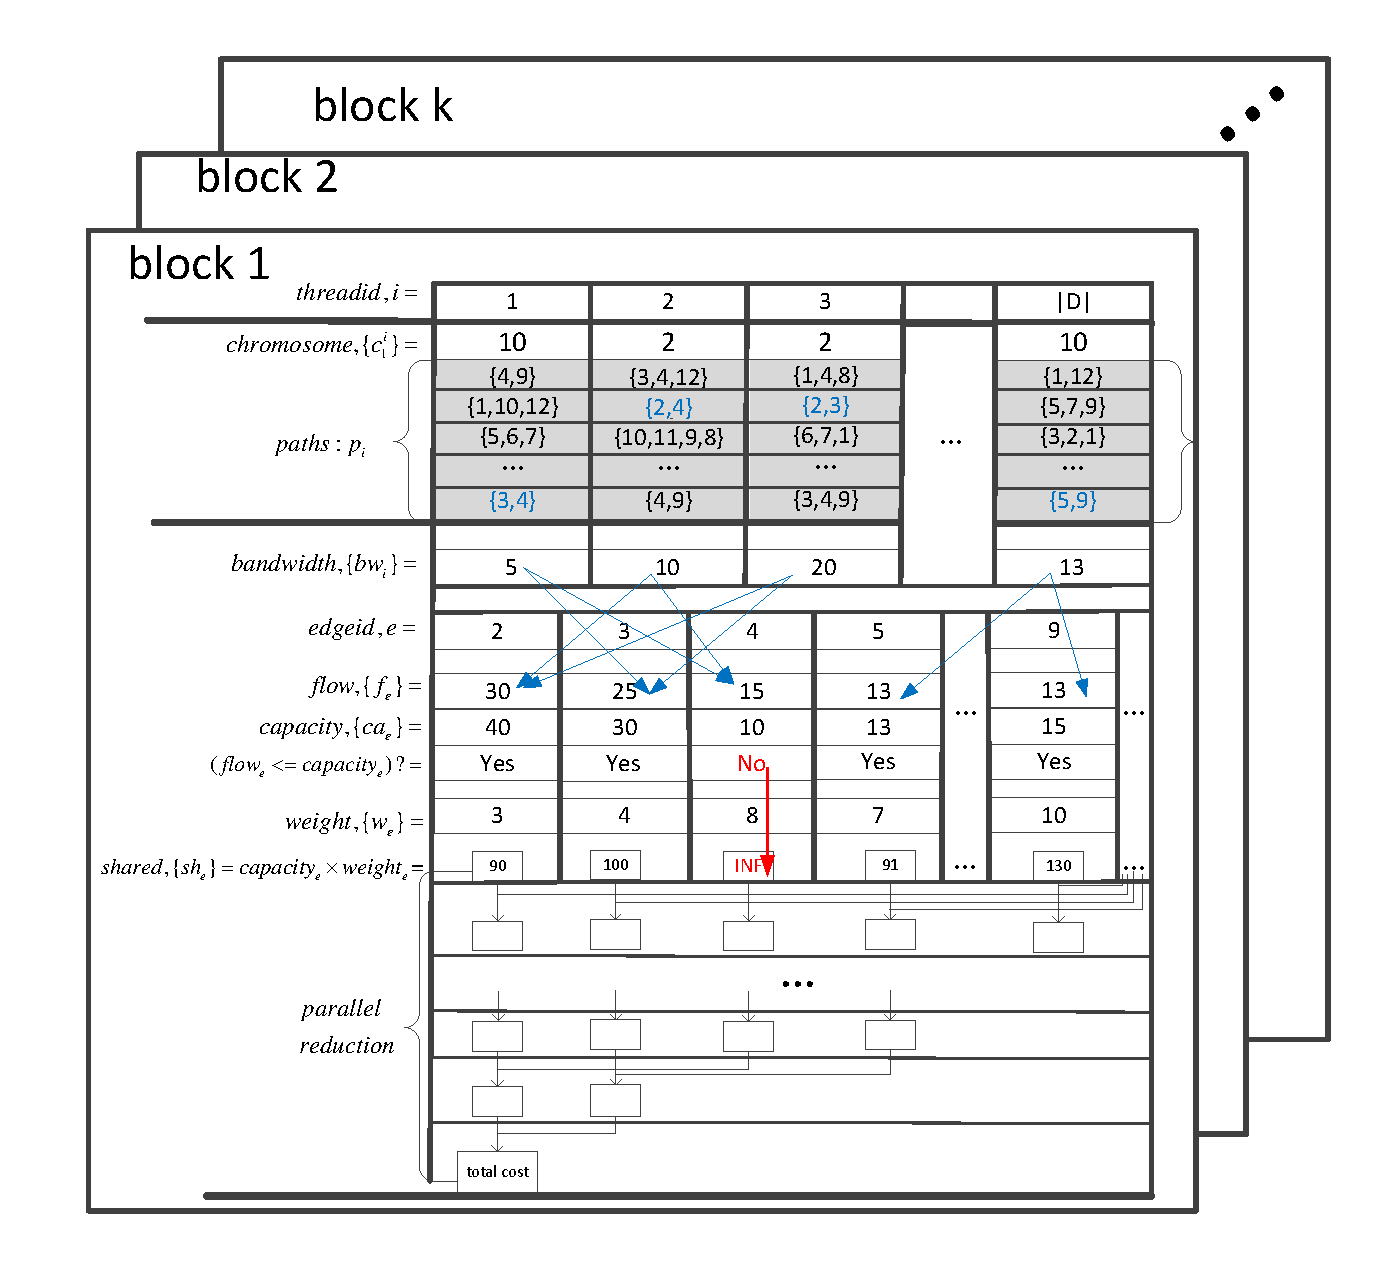
\includegraphics[width=1 \textwidth]{figures/GPUfitness.pdf}}
    \end{center}
  \caption{{\footnotesize{GPU上遗传算法评价函数计算过程图}}}
  \label{fitness}
\end{figure}
符号解释:

染色体(chromosome)基因编号:$c^d_i$表示第$i$个染色体的第$d$个基因位置。

备选路径集合(paths),$p_i$表示第$i$业务的所有备选路集合。

业务带宽(bandwidth),$bw_i$表示第$i$个业务需要的带宽大小。

链路流量(flow),$f_e$表示第链路$e$上占用的流量大小。

链路单位代价(weight),$w_e$表示链路$e$上的代价。

共享内存中间数组(shared),$sh_e$表示链路$e$上的总代价。

如图所示,由于每个染色体的计算过程是独立的,算法为每一个染色体开辟一个block,每个block 内部每个线程负责染色体上的相应业务,首先通过寻址备选路径集合找到这个业务选择的路径,路径上的每一个链路都需要被占用流量,于是遍历这条路径,将业务的流量加到相应的链路上,所有线程同时计算,最后得到链路上占用的流量大小为数组$flow$, 并行比较$flow$ 和$capacity$数组,如果某一线程发现容量超限,则设置链路代价为无穷大(INF)表示此染色体不可行,最后对得到的链路代价数组进行求和,求和采用GPU 上经典的并行规约算法,最后得到染色体对应的效用函数值。

其中$flow$和$shared$两个数组被同一个block内部的线程多次访问,利用程序访问的局部性,将两个数组分配到共享内存中,这样避免了对global memery的大量慢速访问,大大提高程序计算速度。
\begin{lstlisting}[caption={遗传算法并行评价代码},captionpos=b,firstnumber=1,label={GAF}]
void evaluate(float*capacity,
		   float*bandwith,
		   float*weight,
		   int chromsome[][],
		   int paths[][]
		   int &objective[]){

__shared__ float flow[E]={};
__shared__ float shared[E]={};
for(i=threadid;i<|D|;i+=blockDim){
	int p[]=paths[i][chromsome[blockid][i]];
	for(j=0,j<length_of(p);j++)
		{
		int band=bandwidth[blockid];
		atomicAdd(&flow[p[j]],band);
		}		
}
__syncthreads();
for(i=threadid;i<E;i+=blockDim)
{
	if(flow[i]<capacity[i])
		shared[i]=flow[i]*weight[i];	
	else
		shared[i]=INF;	
}
__syncthread();
for(int s=E;s>1;s=(s+1)/2)
{	if(e<s/2)
		shared[e]+=shared[e+(s+1)/2];
	__syncthreads();
}
if(threadid==0)
	objective[blockid]=shared[0];
}
\end{lstlisting}
以上代码\ref{GAF} GPU上的评价过程伪代码,算法开始时先开辟两个大小为边数大小的共享内存数组,然后每个线程负责一个基因点,寻址基因点选择的路径,对路径上的每一条边的流量加上业务的流量大小,注意到这个时候可能同时存在多个线程访问同一个$flow$位置,所以需要同步保护,使得每个线程的加法操作都能正确执行,使用CUDA 提供的atomicAdd函数来对$flow$数组进行加法操作,atomicAdd 保证其调用的操作是原子操作,从而多个线程对同一$flow$位置的加法操作必修是串行执行的,一个add 操作必修一次性执行完成(取址、译码、执行、访存、写回),在当前add操作执行完成之前,其他线程的add 操作必修排队等待。$blockDim$ 表示一个block内的线程数量,代码中的for循环每次迭代标号$i$偏移$blockDim$ 的长度,这是因为业务量数$|D|$可能大于$blockDim$, 如果这样的话,每个线程可能会负责多个业务的统计计算,每个业务标号相差$blockDim$ 大小。

当线程$flow$大小统计完成之后,必修进行同步(syncthreads()),同步操作保证block内部的所有线程执行到同一步骤,也就是统计完成的线程必修等待其他统计线程都执行完成后才能继续执行,因为只有所有线程都完成对$flow$ 数组的加法操作,$flow$ 数组的统计才完整,才能够进一步进行比较操作。
  
代码第19到25行计算每一条链路的路由代价,并把结果储存在$shared$数组中,如果链路上的流量小于其容量约束,那么链路代价就等于单位代价$weight$和链路流量$flow$的乘积,反之,如果流量超限,就设置$shared$为无穷大。同理,当线程计算完成后必修进行同步(syncthreads())操作,以使得shared数组正确完整。	

为了充分利用GPU多线程,代码最后进行并行规约操作进行求和,for循环中每次将后一半的$shared$ 数组加到前一半,规约过程中必修进行同步(syncthreads()),以保证加法过程计算完整,最终求和值规约到一个下标0,将shared[0] 中的值写入到$objective$ 数组中。

另外,由于CUDA每个block支持的shared memory 大小有限,并且分配shared memory太多,会使得SIMT上的资源不足,一个block 中的活跃warp 数量不足,造成SIMT上不能有足够的活跃warp 数量来进行切换,从而掩藏其他warp 的访存延迟开销,这样会使得执行速度下降很多,所以在实际设计计算时$flow$和$shared$使用的是同一段共享内存。
\subsubsection{并行排序,变异与交叉}
由于遗传算法中最消耗时间的部分是评价部分,本设计中对其他部分的并行步骤采用较简单的算法。在评价部分结束后,需要对所有的染色体按照效用函数的大小降序排序,本文采用GPU上的odd-even算法进行排序操作,odd-even 算法的计算过程如下图\ref{oddeven}所示:
\begin{figure}
  \begin{center}
    {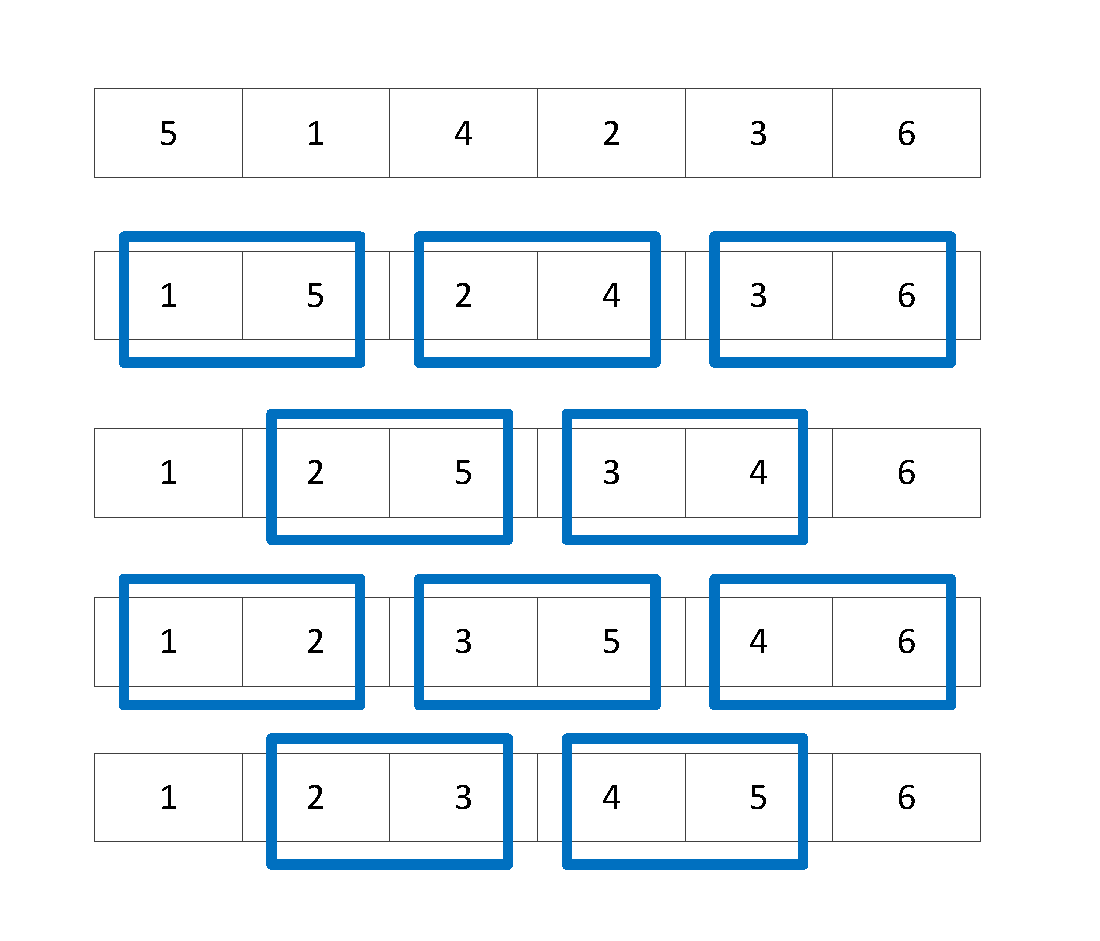
\includegraphics[width=0.8\textwidth]{figures/odd-even.pdf}}
    \end{center}
  \caption{{\footnotesize{并行奇偶排序例子}}}
  \label{oddeven}
\end{figure}

如图所示,奇偶排序算法每次两两比较数组中的值的大小,然后将较小的那个值交换到前面,奇数次的时候比较下标为$2k 和2k+1$ 的值,其中$k \in [0,POP/2]$,偶数次的时候比较下标为$2k-1和2k$的值,其中$k \in[1,POP/2]$,最终经过$POP/2$轮的奇偶比较,就可以得到排序好的数组,从奇偶排序的执行过程可以看出,每一轮比较中的$POP/2$次比较是是相互独立无关的,其具有天然的可并行性,而且其并行实现较简单。
绍染色体排序算法的GPU代码实现如下 \ref{GAS}:
\begin{lstlisting}[caption={并行排序算法},captionpos=b,firstnumber=1,label={GAS}]
\begin{lstlisting}[language=C],
void sort_kernel(float*objective,
	     int**chromsome,
	     int round)
{
int id=2*threadid;
if(round/2==0)
  if(objective[id]<objective[id+1])
  {
	swap(objective[id],objective[id+1]);
	swap(chromsome[id],chromsome[id+1]);
  }
else
  if(objective[id-1]>objective[id])
  {
	swap(objective[id-1],objective[id]);
	swap(chromsome[id-1],chromsome[id]);
  }
};
void sort(float*weight,
	     int**chromsome,
	     int round,
		int POP
		)
{
for(int i=0;i<POP/2;i++)
    sort_kernel(objective,chromsome,i);
}
\end{lstlisting}

如代码 \ref{GAS} 所示,sort函数一共需要执行$POP/2$轮比较,也就要调用kernel\_sort共POP/2次,在kernel\_sort中,一个线程负责两个数的比较与交换操作,在寻址数组之前,要判断当前的比较轮次的奇偶性,如果为奇数,则当前标号为$threadid$ 的线程要去比较标号为$2*threadid$ 和标号为$2*threadid+1$的目标值,如果当前标号为偶数值,则去比较下标为$2*threadid-1$和$2*threadid$ 的值,如果出现较小的值在后面,需要进行交换操作,交换操作在交换$objective$ 数组的同时,也要交换相应的染色体($chromsome$) 数组,这样一轮比较达到并行度为$POP/2$,一个有$POP/2$个线程参与比较交换计算,因为要循环$POP/2$ 次才能保证排序完毕,所以算法总的计算复杂度为$O(POP)$。

交叉过程分为父母选取和交叉计算两个kernel,父母选取过程随机并行地选取$\beta+\gamma$对父母,每个线程负责选取一对父母,并且将选取的父母下标记录到$father$和$monther$数组中,父母选取GPU计算示意图如下图\ref{pp}所示:
\begin{figure}
  \begin{center}
    {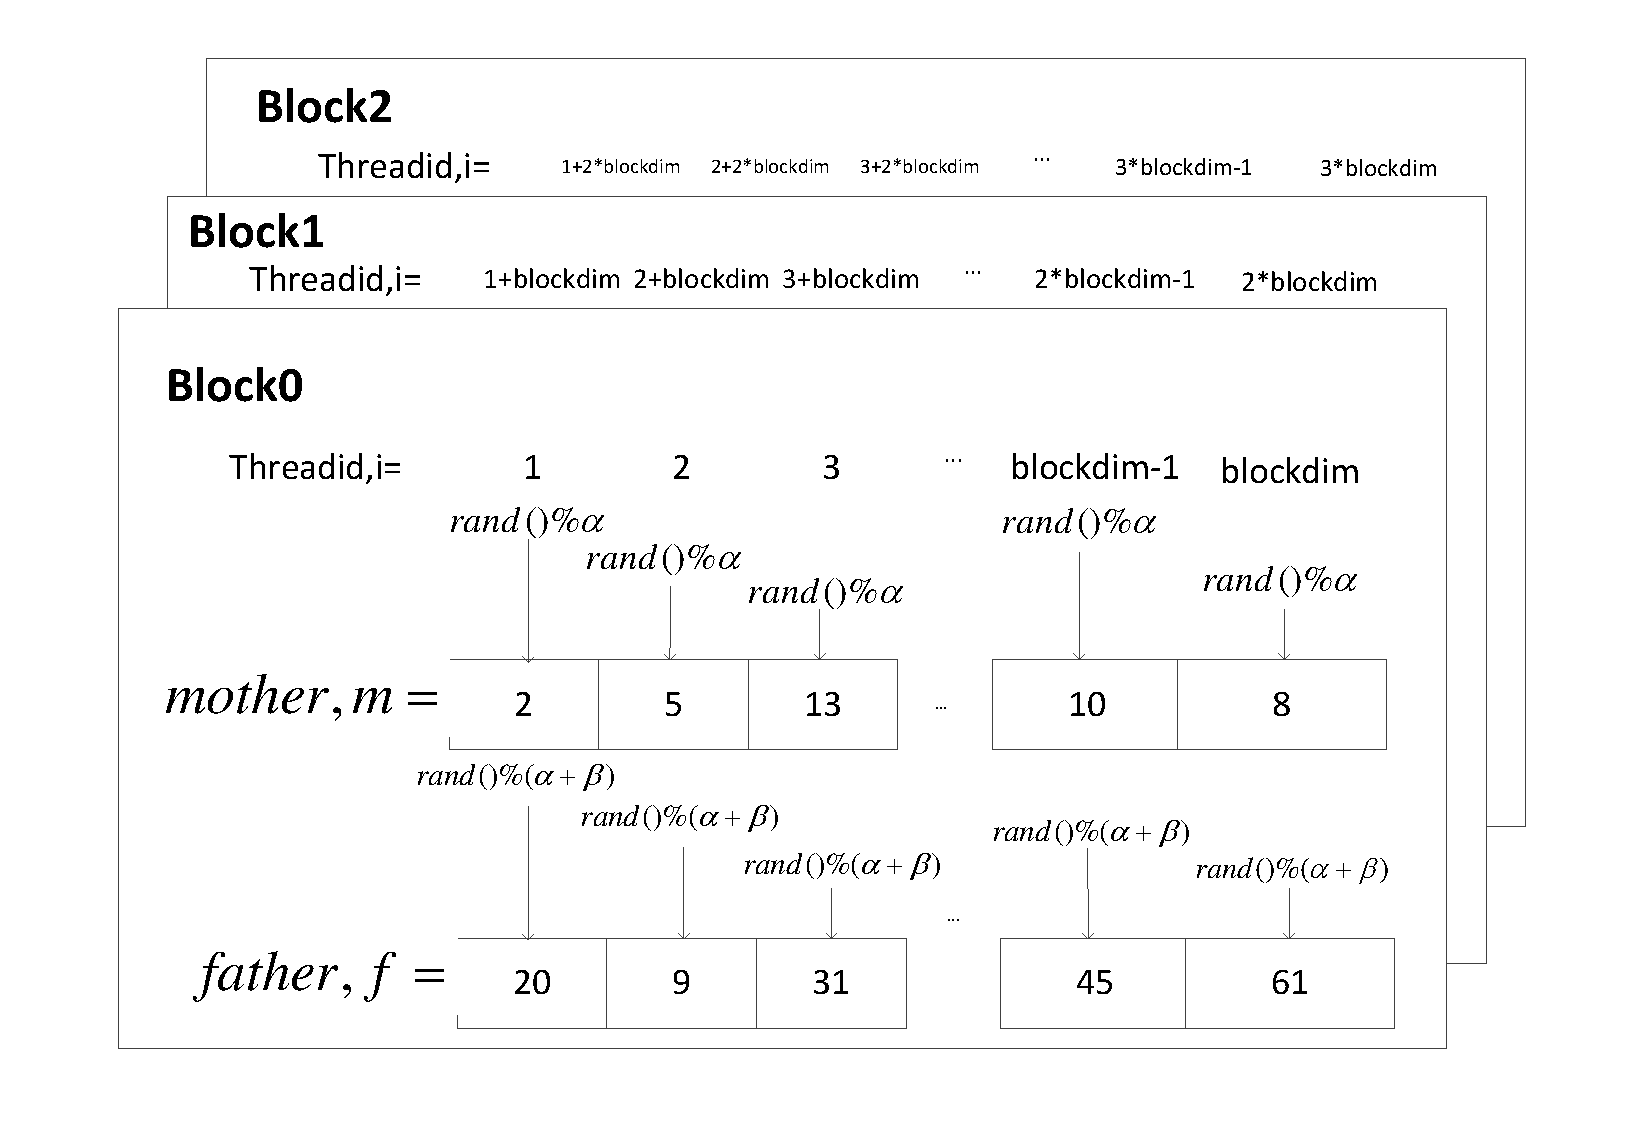
\includegraphics[width=0.8\textwidth]{figures/choose.pdf}}
    \end{center}
  \caption{{\footnotesize{GPU并行父母选取过程}}}
  \label{pp}
\end{figure}
每个线程进行两次随机,$mother$标号只能在前$\alpha$个精英染色体中选取,$father$表号的选取在前$\alpha+\beta$ 中选取,这样既能够给予精英染色体更大的交叉几率,也可以保证解的搜索空间变化足够大,避免陷入局部最优值。

父母选取过程结束后,在GPU端记录了所选取的$mother$和$father$数组,$mother$和$father$数组将用于交叉部分的计算,交叉部分的并行粒度更高,其中每个基因点的计算都是并行执行的,如下图 \ref{cross} 所示:
\begin{figure}
  \begin{center}
    {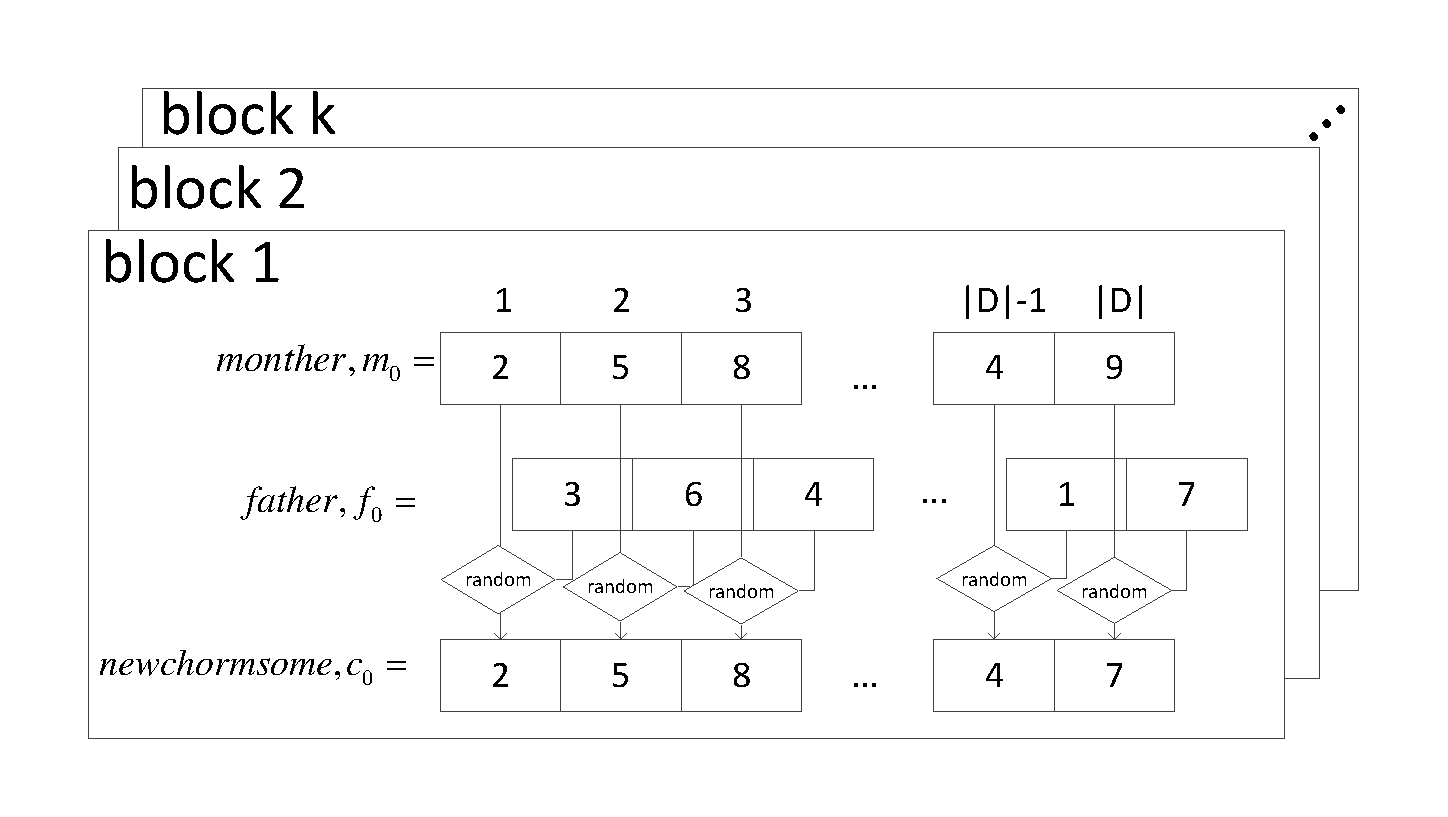
\includegraphics[width=0.8\textwidth]{figures/GPUcross.pdf}}
    \end{center}
  \caption{{\footnotesize{GPU并行均匀交叉过程}}}
  \label{cross}
\end{figure}
每个block负责一个新染色体的生成,通过之前的分析,一共需要生产$\beta+\gamma$个新的染色体,所以GPU 端一共需要分配$\beta+\gamma$ 个block,其中每一个block中有|D| 个线程来同时负责随机从$monther$和$father$ 的相应点位选择一个来作为新染色体相应点位的值,如前所说采用均匀交叉策略,选择父亲母亲遗传基因的概率都是50\%,这样,这样block 内部的并行度达到$|D|$,总的并行粒度达到$|D|*(\beta+\gamma)$。
\begin{lstlisting}[caption={并行交叉算法代码},captionpos=b,firstnumber=1,label={GAC}]
void cross_kernel(float*monther,
			  float*father,
	     		  int**chromsome,
                  int**newchromsome
			  )
{
int mid=monther[blockid];
int fid=father[blockid];
int a=chromsome[mid][threadid];
int b=chromsome[fid][threadid];
int mark=rand()%100;
if(mark<50)
  newchromsome[blockid+alpha][threadid]=a;
else
  newchromsome[blockid+alpha][threadid]=b;
}
\end{lstlisting}

上面代码 \ref{GAC} 为CUDA上实现的均匀交叉伪代码,kernel输入为已经随机选好的$monther$和$father$ 数组,线程进入函数先找到block 对应的母亲和父亲的染色体id,通过id寻址到相应的染色体编号,通过threadid寻址到当前的基因位置,然后随机产生一个0 到100的数,此数如果小于50,则选择继承母亲的基因,反之,则继承父亲的基因,需要注意的是新生成的染色体数组($newchormsome$数组),其前$\alpha$个染色体直接复制排序后染色体集合的前$\alpha$ 个染色体,也就是说前面的$\alpha$ 个精英染色体直接保留到下一轮,所以代码中交叉产生的新染色体基因在填入$newchormsome$数组中时,需要偏移$\alpha$ 个单位。

最后,对于变异部分,由之前的分析可知,变异步骤的计算量不大,并行粒度也不高,所以其并行算法实现不再赘述。
\section{基于拉格朗日的优化算法设计}

基于遗传算法的路由优化算法,虽然过程简单,但是其具有以下缺点,第一,需要事先计算大量备选路径,不能很好地适应网络的动态变化,一旦网络链路发生变化,又要重新计算备选路径。第二,遗传算法从开始到收敛需要大量的迭代次数,虽然经过GPU加速计算,但是由于收敛缓慢,任然需要大量的计算时间,迭代次数,很大程度上是决定于初始染色体集合的好坏,而随机选择路径的方式很难得到好的初始集合。第三,遗传算法容易陷入局部最优解,交叉范围小,和变异范围小都会使得算法提前陷入局部最优解,而如果交叉范围太大,变异范围太大,又会使得算法收敛缓慢,而且路由优化问题中每一个业务都有大量备选路径,问题的解空间很大,即使增大搜索范围也很难找到更优化的解。于是本节通过分析采用基于拉格朗日乘子法的GPU并行方法来求解路由优化问题。
\subsection{问题建模}
  路由优化问题就是为每一个业务选取一条路径,以使得效用函数最小化。然而在MILP模型中,网络容量约束,把所有的路由变量联系到一起,因为这些变量的取值必修保证每一条链路$(i,j)$上占用的流量小于其容量$\beta\cdot c_{ij}$,正是由于存在链路容量约束,每个业务的路由选取才变得不相互独立,但是要利用GPU 的并行特性,需要寻找独立计算的可能性,因此,本文采用拉格朗日松弛方法,把一个路由优化问题分解成一些单个业务的寻路问题,而这些单业务的寻路问题是相互独立的,很适合并行计算。将问题。。中的网络容量约束松弛进目标函数得到如下问题:
\begin{equation}\label{LagProb}
\begin{split}
L(\mathbf{\lambda})= min\sum\limits_{d \in D}\sum\limits_{(i,j) \in E_a} w_{ij}x_{ij}^d bw_d+ \\ ~~~~~\sum\limits_{(i,j) \in E_a}\lambda_{ij}(\sum\limits_{d \in D} (x_{ij}^d bw_d-\beta c_{ij})
\end{split}
\end{equation}
其中 $\lambda_{ij}$ 表示链路 $(i,j)$的拉格朗日乘子。
这个表达式(\ref{LagProb})还可以表示为:
\begin{equation}\label{Lagprob1}
L(\mathbf{\lambda})= min\sum\limits_{d \in D}\sum\limits_{(i,j) \in E_a} (w_{ij}+\lambda_{ij})x_{ij}^dbw_d -\sum\limits_{(i,j) \in E_a}\lambda_{ij}\beta c_{ij}
\end{equation}
subject to:
\begin{equation}\label{FlowConv2}
\begin{split}
\sum\limits_{(i,j) \in E_a} x_{ij}^d - \sum\limits_{(j,i) \in E_a} x_{ji}^d
=\begin{cases}
1 & \text{if $i = s_d$}\\
-1 & \text{if $i = t_d$} \\
0 &{ohterwise}
\end{cases}
\\~~~~~~~~\forall i\in V_a, \forall d\in D
\end{split}
\end{equation}
 拉格朗日子问题的目标函数中的$\sum_{(i,j) \in E_a}\lambda_{ij}\beta c_{ij}$这一项,不随着拉格朗日乘子的变化而变化,本文将其作为常数项而丢掉不讨论,丢掉$\sum_{(i,j) \in E_a}\lambda_{ij}\beta c_{ij}$ 这一项后,拉格朗日子问题的目标函数中只含有代价部分 $w_{ij}+\lambda_{ij}$和$x_{ij}^d$的乘积。注意到,$\sum_{(i,j) \in E_a} (w_{ij}+\lambda_{ij})x_{ij}^d bw_d$表示业务$d$ 的总路由代价,因此,拉格朗日子问题的目标函数是最小化所有业务需求的路径路由代价总和,在这个子问题的约束中,没有一个约束同时包含有两个及以上的业务需求相关的变量,所有这个拉格朗日子问题可以被分解成一系列独立的最短路径问题(每个业务需求对于一个最短路问题),只是这些最短路问题的链路单位代价发生改变,链路代价变得和拉格朗日乘子 $\mathbf{\lambda}$ 相关,也就是说给定一个拉格朗日乘子$\mathbf{\lambda}$,我们可以通过并行地计算一系列的最短路径问题来解决这个拉格朗日子问题。
因为把容量约束松弛进效用函数中后,不会增加目标函数的值(<0), $L(\mathbf{\lambda})$成为原问题最优目标函数值的下界,$z^* \ge L(\mathbf{\lambda})$,为了得到最紧的的下界值,我们要解决以下这个优化问题:
 \begin{equation}\label{dual}
L^*(\mathbf{\lambda^*}) = maximize_{\mathbf{\lambda}}L(\mathbf{\lambda})
\end{equation}
~~~subject to: (\ref{FlowConv2})
 \vskip 0.2cm

以上的这个优化问题也被称为原来路由优化问题的对偶问题(),其中$\mathbf{\lambda}$ 表示最优拉格朗日乘子,为了得到最优乘子$\mathbf{\lambda^*}$,可以使用次梯度优化算法来解决,次梯度优化计算时,第一次先初始化乘子 $\mathbf{\lambda}^0$, 然后通过以下过程进行迭代求解:
\begin{equation}\label{iter}
   \mathbf{\lambda}_{ij}^{(k+1)} =\mathbf{\lambda_{ij}}^{(k)}+\theta_{k} g^{(k)}= \mathbf{\lambda_{ij}}^{(k)} + \theta_k[(\sum\limits_{d \in D}x_{ij}^d - c_{ij})]^+
\end{equation}
其中, $\mathbf{\lambda}_{ij}^{(k)}$表示第$k$次迭代的对应于边$(i,j)$的拉格朗日乘子, $g^{(k)}$是$L(\mathbf{\lambda})$ 对$\mathbf{\lambda}^{k}$的任意一种次梯度,$\theta_k$ 表示第$k$次的迭代的步长,标记$[\alpha]^+$ 表示$\alpha$中符号为正的部分,也就说$[\alpha]^+=max(\alpha, 0)$,从表达式可以看出来如果链路$(i,j)$ 上的流量总和超过链路$(i,j)$上的容量,链路$(i,j)$ 上的$\lambda_{ij}^k$拉格朗日乘子会增加,也就是表示一些业务流量需要从链路$(i,j)$上移除,另外,为了避免产生负权重的链路代价,当链路容量大于其上的流量时,我们并不去减小此链路$(i,j)$上的$\lambda_{ij}^k$。
 根据以上讨论,我们给出基于拉格朗日乘子法的并行路由优化算法的框架,如图\ref{lpl}所示,LR-PTEA主要包括以下步骤:步骤一,为$G_a(V_a, E_a)$ 初始化链路权重。步骤二,计算所有业务的最短路径,其中路径计算任务被分配到GPU 进行并行计算。进一步,为了充分利用GPU的大规模计算能力,一种基于GPU 的并行最短路算法被用来为每个业务计算路径。步骤三,为了从当前计算出来的路径中得到更好的目标函数值,对步骤二中计算出来的路径进行调整。步骤四,更新链路权重,更新完毕后,如果停止条件不满足,则回到步骤二,进入下一轮迭代。LR-PTEA 如果在连续$\beta$次成功的迭代后依然不能找到更优的全局解,则停止算法过程。
\begin{figure}
  \begin{center}
    {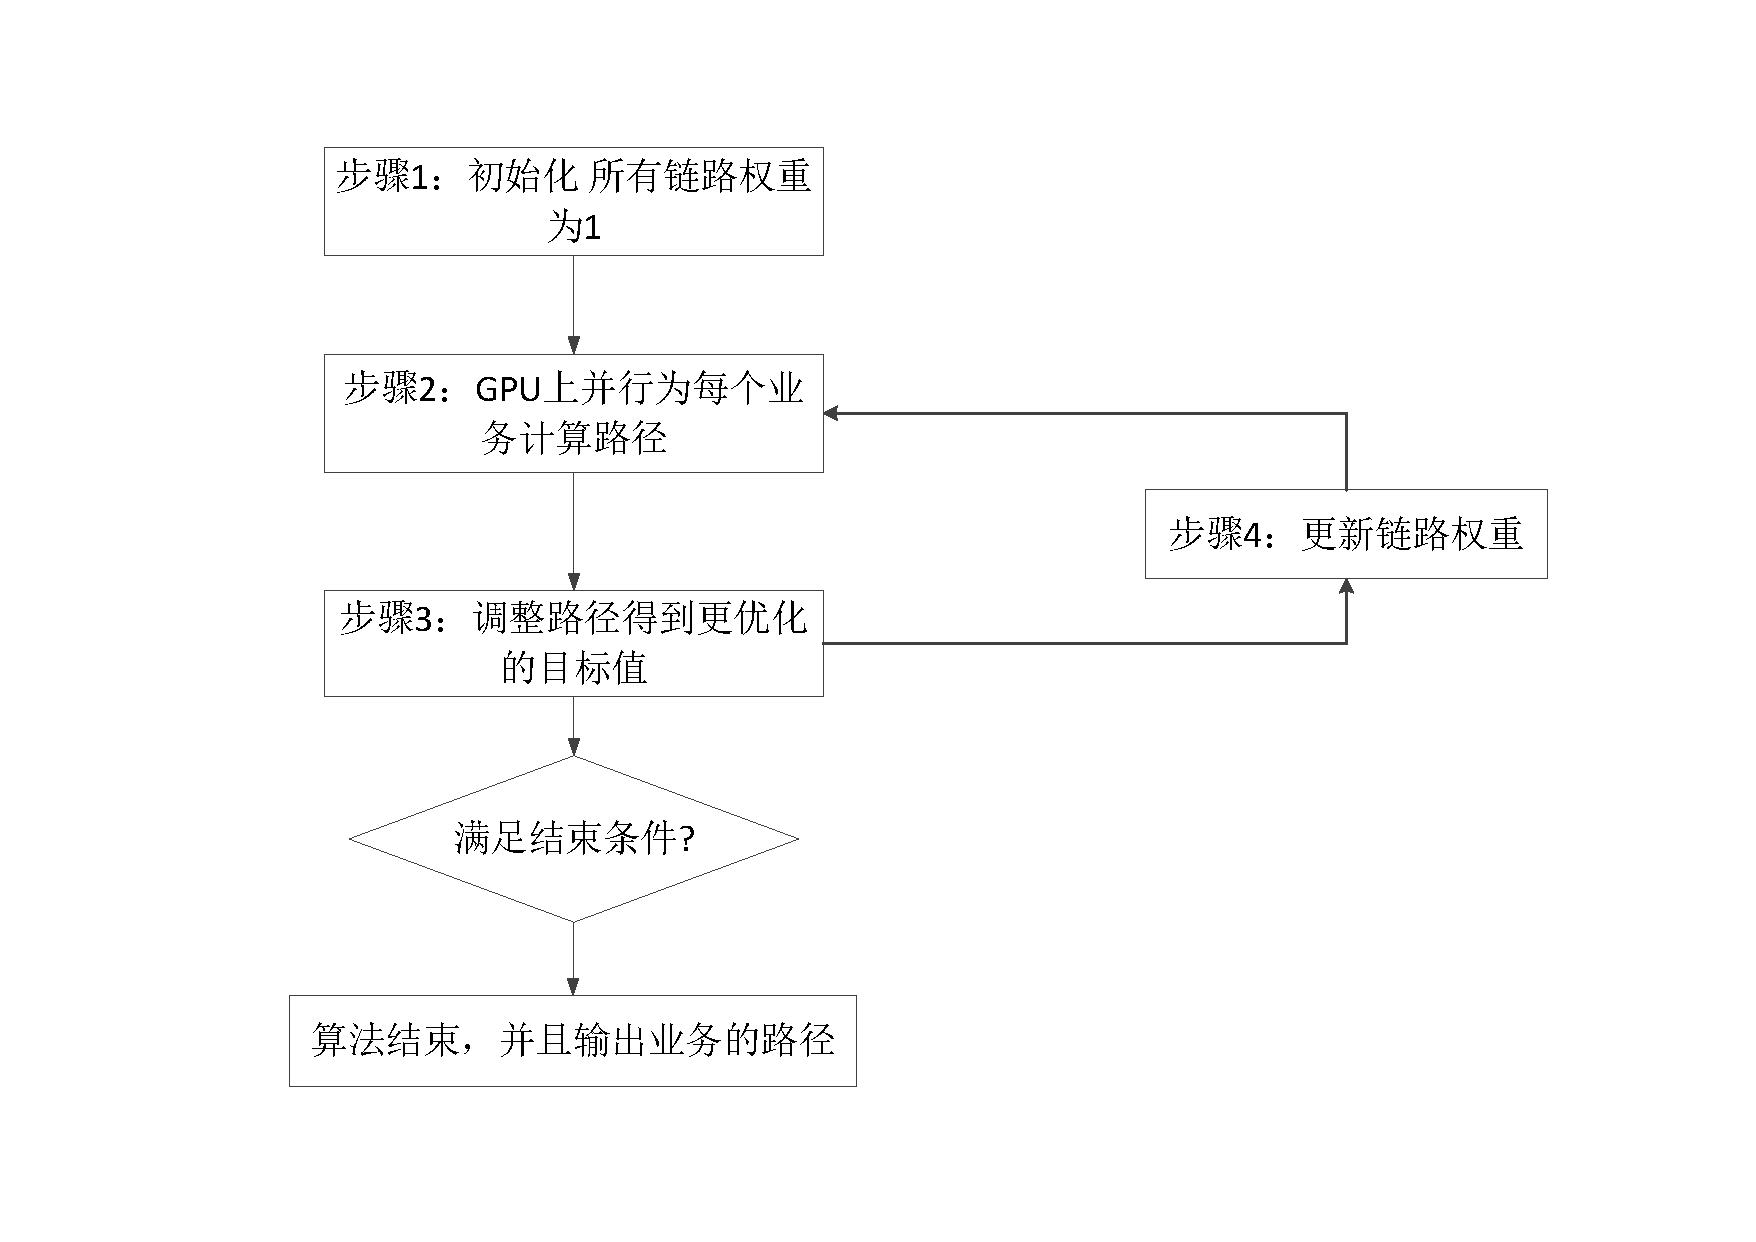
\includegraphics[width=1\textwidth]{figures/lagrange.pdf}}
    \end{center}
  \caption{{\footnotesize{LR-PTEA算法流程图}}}
  \label{lpl}
\end{figure}
\subsection{基于GPU的并行路由计算}
  在每次迭代中,LR-PROA为每个业务 $d \in D$在图 $G_a(V_a, E_a)$中计算最短路径,显然,丢掉链路容量约束后,不同业务的最短路径计算可以独立在GPU上并行执行,但是,最短路算法的逻辑对于GPU来说太过复杂,GPU最初是被设计来做大规模的数值计算问题,其只实用于逻辑比较简单,但是数值计算量较大的任务,所以在GPU上直接开辟一个线程来计算一个业务的路径,不仅仅在计算上是低效的,而且这样的并行粒度也不能充分利用GPU 的大规模并行能力。为了充分提高最短路径的计算速度,LR-PROA 对最短路径算法进行并行化设计。
\begin{algorithm}[htb]
\caption{{Bellman最短路算法}}
\label{Bellman}
\begin{algorithmic}[1]
\Require
网络拓扑:$G(V, E)$;
源点:$s$;
\Ensure
从$s$开始到其他点的路径集合$P$;
\For {each node $v \in V$}
\State {$Dist[v] \leftarrow \infty$}
\State {$Pre[v] \leftarrow $ NIL}
\EndFor
\State {$Dist[s] \leftarrow 0$}
\State {$Mark \leftarrow 1$}
\While {$Mark > 0$}
\State {$Mark \leftarrow 0$}
\For{each link $(u,v) \in E$}
\If{$Dist[v]>Dist[u]+w_{uv}$}
\State {$Dist[v] \leftarrow Dist[u]+w_{uv}$}
\State {$Pre[v] \leftarrow u$}
\State {$Mark = 1$}
\EndIf
\EndFor
\EndWhile
\State {根据前驱数组$Pre$,重新构建最短路集合,输出路径到集合$P$}
\Return {$P$}
\end{algorithmic}
\end{algorithm}
  
文章[]提出一种Dijkstra最短路径算法在GPU上的并行实现,但是从算法结构上分析,Dijkstra最短路径算法并不适应于并行算法的设计,所以Dijkstra最短路径算法在GPU上的实现不能得到很好的加速效果,为了期望得到更好的加速效果,LR-PROA 选择Bellman-Ford 最短路算法来进行并行实现,Bellman-Ford最短路算法逐步地减小距离标记 $Dist[v],v\in V$,直达其收敛与真实的最短距离。Bellman-Ford算法过程如上图,其中 $Dist[v]$ 表示距离起点$s$到$v$的最短路径距离,$Pre[v]$ 表示点$s$到点$v$ 的最短路径上$v$ 的前驱节点,在初始化好了所以节点的距离数组和前驱节点数组之后,Bellman-Ford算法最多迭代 $|V|$ 次,每一次迭代算法松弛一次图$G(V, E)$ 中的所有的边(第10-11行)。Bellman-Ford 算法的算法复杂度为$(|V|\cdot |E|)$,他的复杂度高于Dijkstra最短路径算法的复杂度,但是,因为Bellman-Ford算法每次松弛边的操作都是独立无关的,通过为每一条边的松弛操作分配一个独立的线程执行,Bellman-For算法很容易在GPU 上实现并行化。
\begin{figure*}
\setlength{\belowcaptionskip}{-0.5cm}
  \begin{center}
    {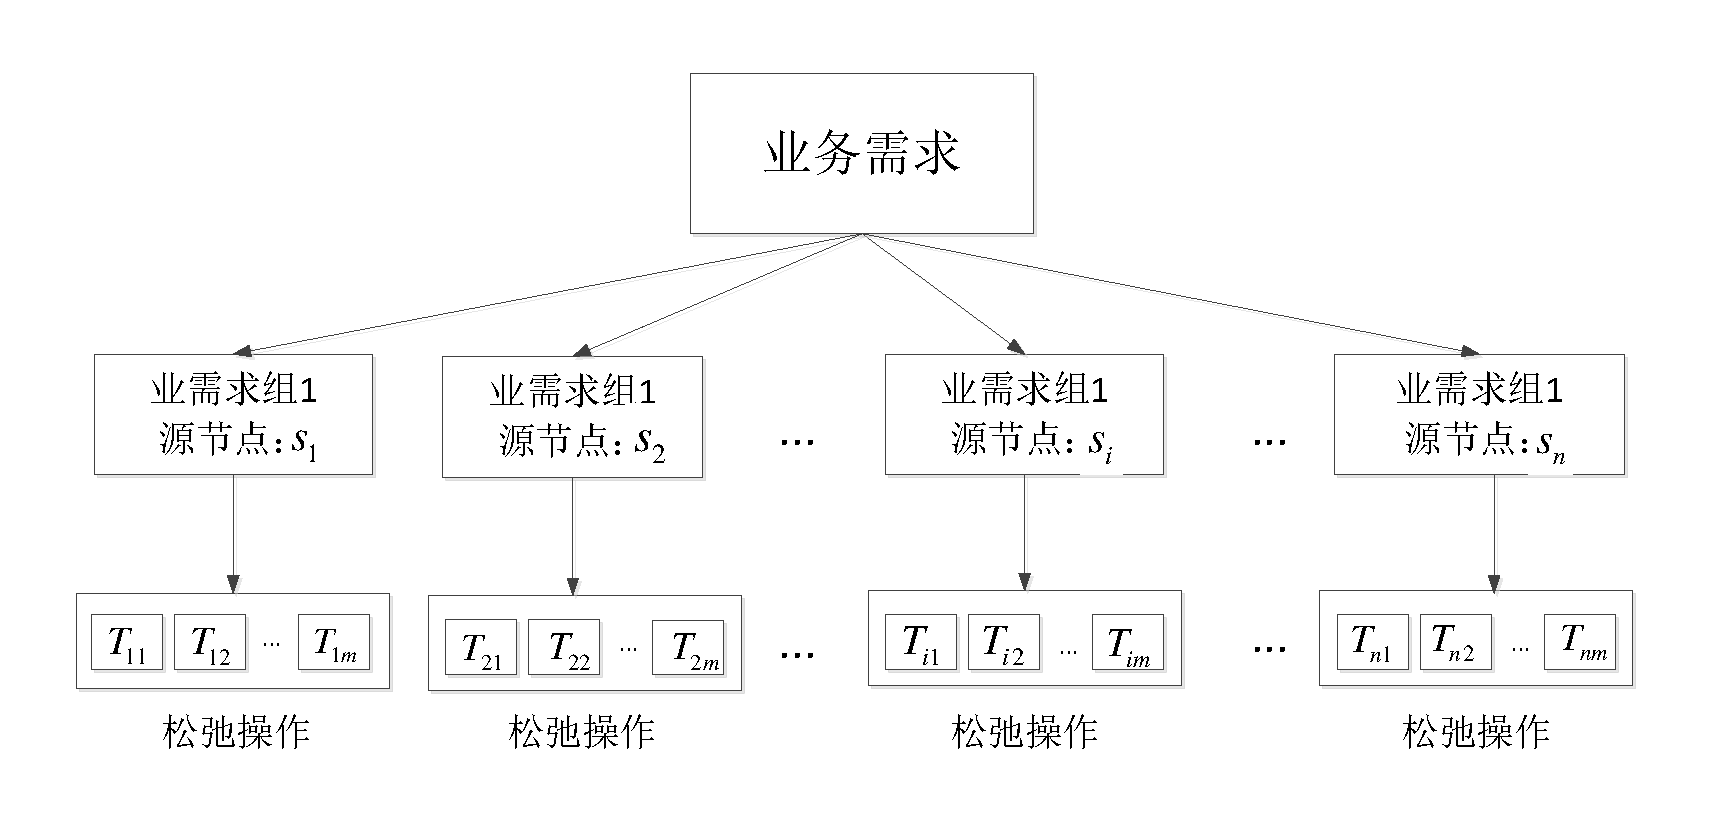
\includegraphics[width=1 \textwidth]{figures/paframework.pdf}}
    \end{center}
  \caption{{\footnotesize{并行业务计算框架}}}
  \label{ParFramework}
\end{figure*}

上图 \ref{ParFramework} 中显示了LR-PROA的最短路径计算的并行实现框架。首先,将业务量需求根据业务的源节点将业务分配成不同的组,使得每一组内的业务的源节点相同。我们假设第$i$个组的源节点为$s_i$。 然后,为了高速的计算最短路径,每一组的最短路径计算使用$m$ 个GPU 线程的并行bellman-ford算法进行计算,如上图\ref{ParFramework}所示,线程$T_{i,j}$负责为对应于源点$s$的链路$e_{j}$ 进行松弛操作。因此总的并行执行的线程数是$m \times k$,其中$m$和$k$分别表示链路数目和组的数目。

在CUDA编程模型中,kernel在执行在一系列的block中,一个block中包含一系列并行执行的线程,在本文的最短路算法并行实现中,每个block内部的线程用于松弛同一条链路$(i,j)$ 的不同源节点情况,比如,在图 \ref{GB} 中,集合$\{T_{1j}, T_{2j}, \cdots, T_{ij}, \cdots, T_{kj}\}$都在bock$j$上执行,其中 $T_{ij}$为对应源节点为$s_i$ 的链路$e_i$ 执行松弛操作,其中,我们设链路$e_i$的头节点和尾节点分别为$h_i$ 和$t_i$,可以看到,当这次迭代存在链路更新,那么标记$Mark$会被设置成一,这是为了优化算法的迭代次数,当某次迭代结束$Mark=0$ 则表示这次迭代没有边进行了更新操作,说明Bellman 算法已经提前结束,实验证明这一个优化可以大大地减小Bellman算法的迭代运行次数。
\begin{figure*}
\setlength{\belowcaptionskip}{-0.5cm}
  \begin{center}
    {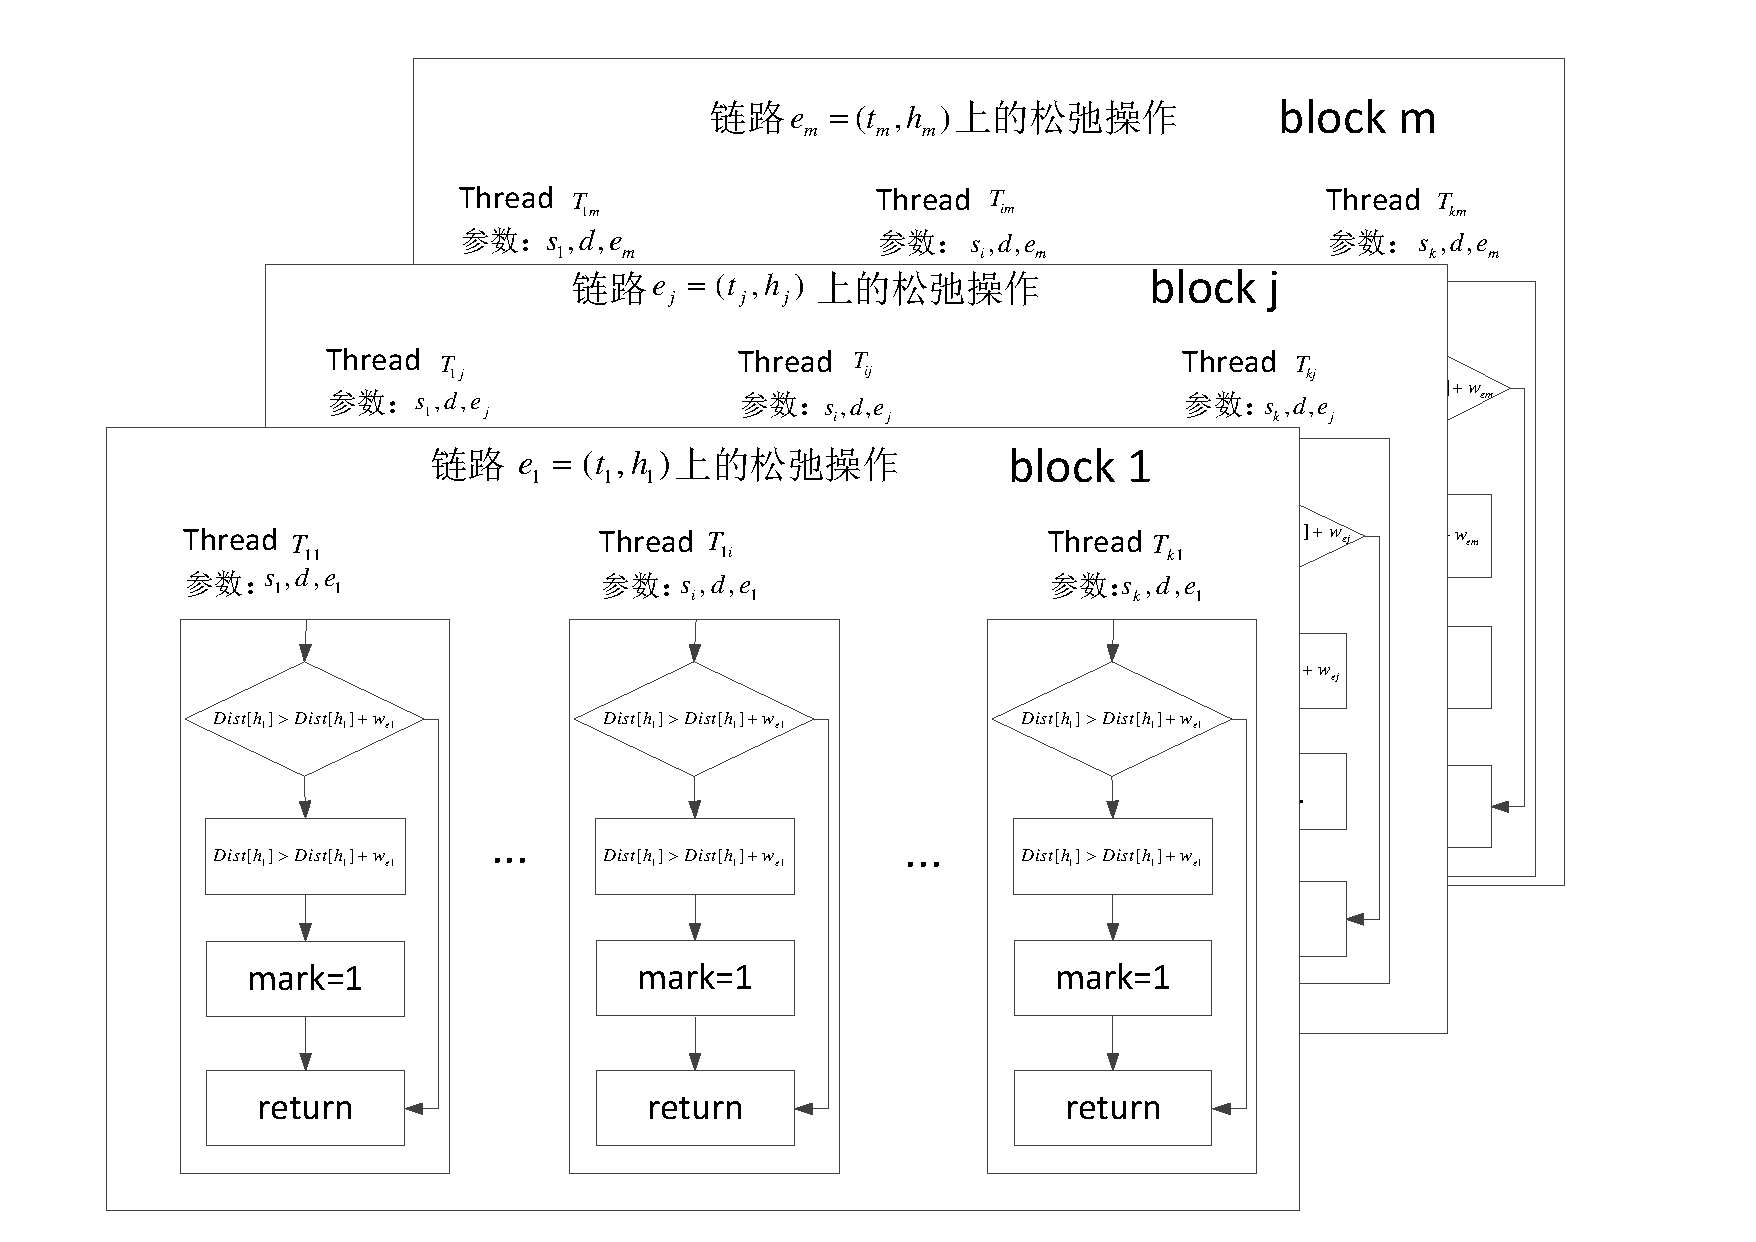
\includegraphics[width=1 \textwidth]{figures/GPUimpl.pdf}}
    \end{center}
  \caption{{\footnotesize{GPU上Bellman算法的实现}}}
  \label{GB}
\end{figure*}

\begin{figure*}
\setlength{\belowcaptionskip}{-0.1cm}
  \begin{center}
    {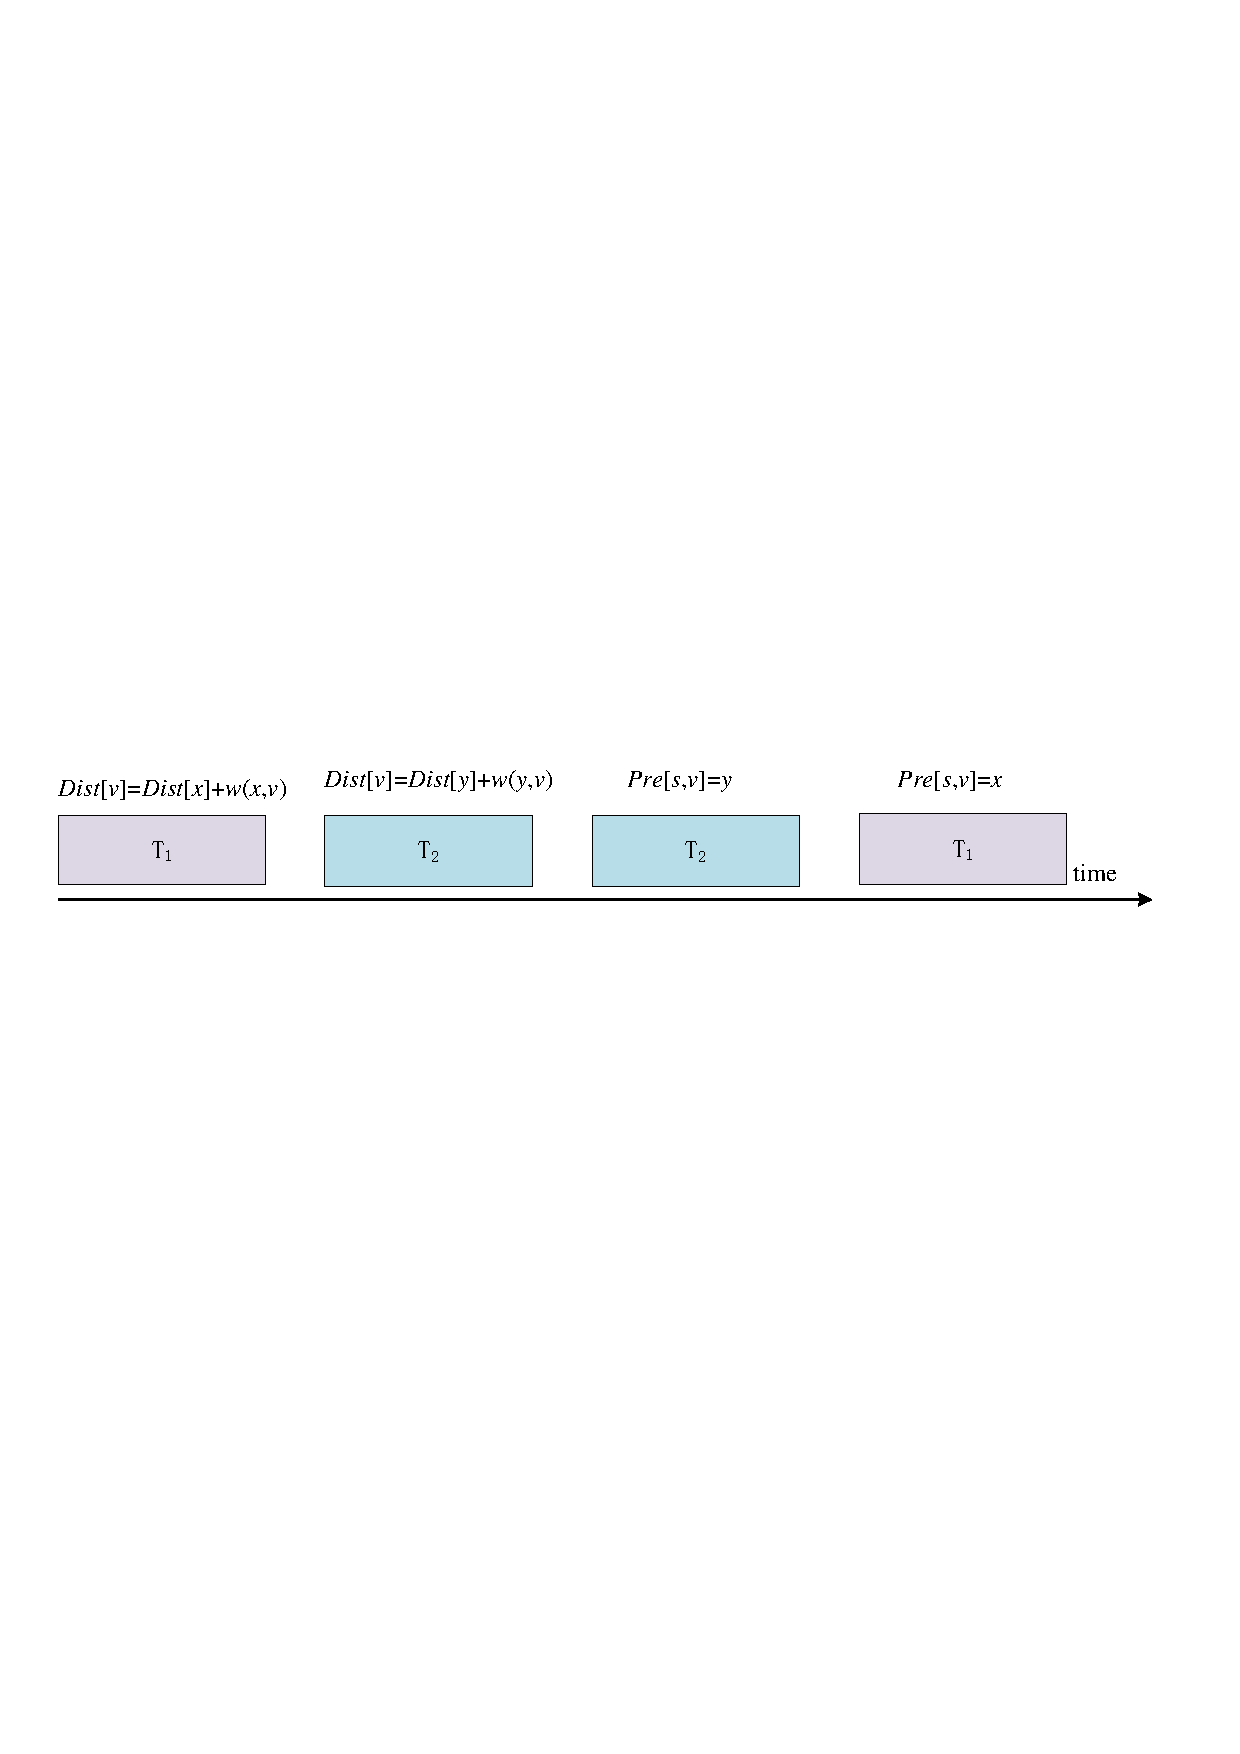
\includegraphics[width=0.8 \textwidth]{figures/SynPro.pdf}}
    \end{center}
  \caption{{\footnotesize{同步问题的例子}}}
  \label{SynPro}
\end{figure*}
最短路径算法CUDA实现算法伪代码如下所示。需要注意的是由于线程在GPU上是独立执行的,在更新节点的距离标记和前驱标记的时候会出现同步问题,假设线程$T_1$为链路$(x,v)$执行松弛操作,而线程$T_2$为链路$(y,v)$ 执行松弛操作,假设两个线程更新点$v$ 的距离标记和更新前驱标记的顺序如 \ref{SynPro} 所示,如果$Dist[y] + w(y, v) < Dist[x] +w(x, v)$,那么$Dist[v]$ 被更新为$Dist[y] + w(y, v)$,但是由于更新的顺序发生交叉,节点$v$的前驱节点被更新成了$x$, 而不是真正正确的前驱节点$y$。为了避免这个同步问题,算法设计中使用两个kernel,一个用来更新距离标号,一个用来更新前驱节点。
\begin{algorithm}[t]
\begin{algorithmic}[1]
\caption{{并行最短路计算}}
\label{ParaSPC}
\Require
	 业务需求集合$D$;
      链路集合$E$;
\Ensure {业务需求的最短路径结合$P$}
\State {将业务的源节点加入到集合$S$中}
\State {$Mark \leftarrow$ 1}
\While{$Mark > 0$}
\State {$Mark \leftarrow$ 0}
 \State {发射 kernel\_distance\_update($S$, $E$, $Dist$)}
\EndWhile
 \State {发射 kernel\_predecessor\_update($S$, $E$, $Dist$, $Pre$)}
 \State {reconstruct the shortest paths for the traffic demands based on predecessor information record in $Pre$, and put the paths to set $P$}
\Return {$P$}
\end{algorithmic}
\end{algorithm}

\begin{algorithm}[t]
\begin{algorithmic}[1]
\caption{\small{kernel\_distance\_update($S$, $E$, $Dist$)}}
\label{KernelDist}
\State {$bid \leftarrow$ block ID}
\State {$tid \leftarrow$ thread ID}
\State {将 $(bid, tid)$ 映射到 id $sid$}
\State {$s \leftarrow S[sid]$}
\State {$e \leftarrow E[bid]$}
\If{$Dist[s][e.tail] + e.weight < Dist[s][e.head]$}
\State {$Mark \leftarrow 1$}
\State {$Dist[s][e.head] \leftarrow Dist[s][e.tail] + e.weight$}
\EndIf
\Return
\end{algorithmic}
\end{algorithm}

\begin{algorithm}[t]
\begin{algorithmic}[1]
\caption{{kernel\_predecessor\_update($S$, $E$, $Dist$,$Pre$)}}
\label{KernelPre}
\State {$bid \leftarrow$ block ID}
\State {$tid \leftarrow$ thread ID}
\State {将 $(bid, tid)$ 映射到 id $sid$}
\State {$s \leftarrow S[sid]$}
\State {$e \leftarrow E[bid]$}
\If{$Dist[s][e.tail] + e.weight = Dist[s][e.head]$}
\State {$Pre[s][e.head]= e.tail$}
\EndIf
\Return
\end{algorithmic}
\end{algorithm}
\subsection{链路权重更新}
\subsubsection{权重更新步长}
  
在LR-PROA算法中,在第$(k+1)$次迭代,链路$(i,j)$的权重被更新为$w_{ij}^{k} + \lambda_{ij}^{k+1}$, 其中$\lambda_{ij}^{k+1}$ 被更新为:
\begin{equation}\label{Iter}
  \lambda_{ij}^{k+1} = \lambda_{ij}^k + \theta_k[(\sum\limits_{d \in D}x_{ij}^dbw_d - \beta c_{ij})]^+.
\end{equation}
  
为了保证收敛性,第$k$次迭代的更新步长($\theta_k$)可以被设置为 $\frac{1}{k}$[]。 然而,通过仿真发现,当($\theta_k$) 被设置为 $\frac{1}{k}$时,其收敛缓慢。让我们考虑图()的例子,其中链路$(i,j)$ 上标记分别表示链路权重和链路上剩余的容量大小。假设现在有两个业务需求($d_1$ 和$d_2$)其源和目的节点都是$A$ 和$D$,且每一个业务的流量大小都是4个单位。为了展示这个迭代过程,我们把算法前5次的迭代结果表示在表() 中,从表中可以看到,业务计算出的最短路径一直在$A-B-D$和$A-C-D$ 之间徘徊。算法必修等到$A-B-D$ 和$A-C-D$ 的两条路的权重相等时才能停止,只有这样这两个业务才可能分离,其中一个选择$A-B-D$,而另一个选择$A-C-D$。 但是,正如表中所示这需要大量的迭代才能达到。
\begin{figure}
\setlength{\belowcaptionskip}{-0.1cm}
  \begin{center}
    {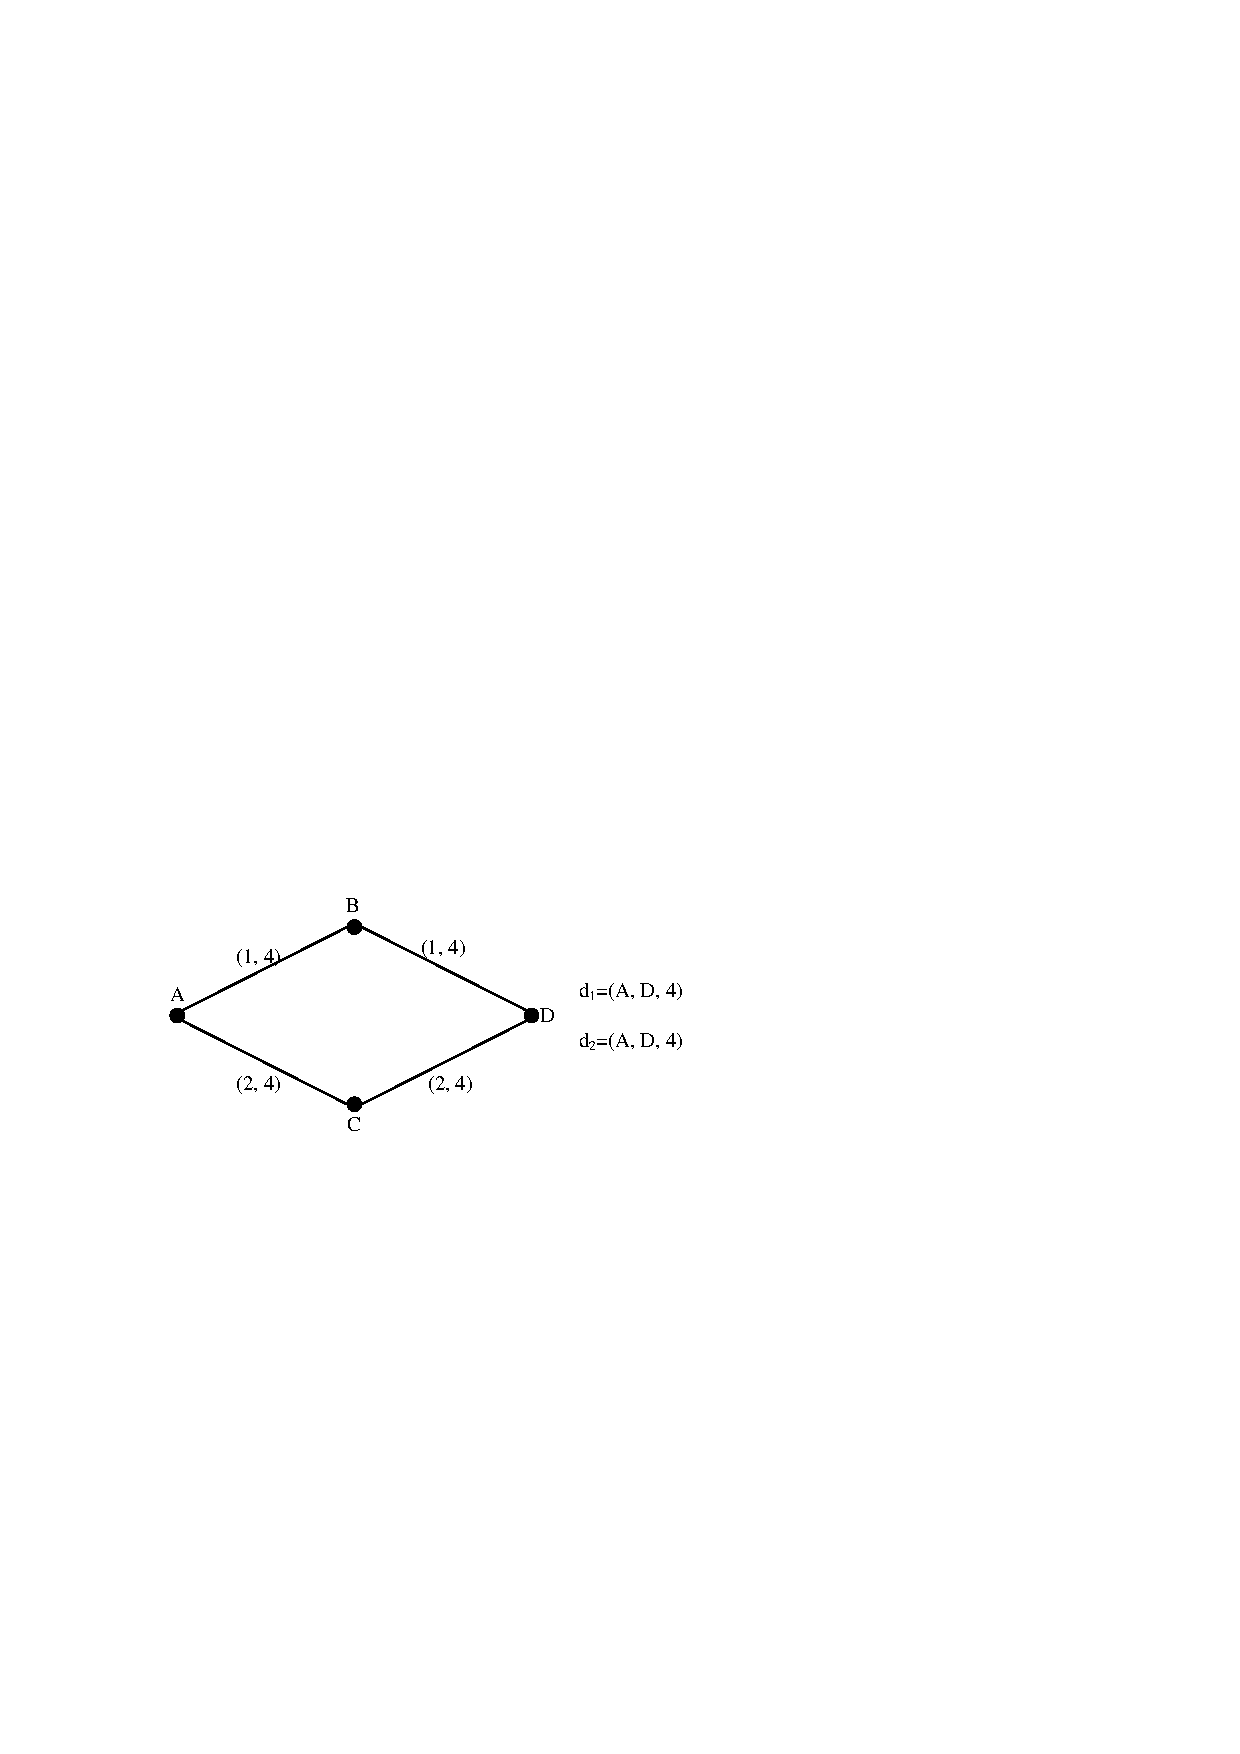
\includegraphics[width=0.4 \textwidth]{figures/IterNum.pdf}}
    \end{center}
  \caption{{\footnotesize{链路更新例子1}}}
  \label{u1}
\end{figure}
\begin{table}[t]
\newcommand{\tabincell}[2]{\begin{tabular}{@{}#1@{}}#2\end{tabular}}
\setlength{\abovecaptionskip}{0.2cm}
  \centering
 \scriptsize{
 \renewcommand{\tabcolsep}{0.09cm}
 \renewcommand{\arraystretch}{1.2}
    \begin{tabular}{| c | c | c | c|}
    \hline
     Iteration number & \tabincell{l}{Calculated paths for \\the two demands} & Path weights & $\theta_k$
\\ \hline
 0 & \tabincell{l}{A-B-D \\ A-B-D} & \tabincell{l}{4(1+1) \\ 4(1+1)} & 1   \\ \hline
1 & \tabincell{l}{A-C-D \\ A-C-D } & \tabincell{l}{4(2+2) \\ 4(2+2)} & 1   \\ \hline
2 & \tabincell{l}{A-B-D \\ A-B-D} & \tabincell{l}{4(1+4+1+4) \\ 4(1+4+1+4)} & 0.5 \\ \hline
3 & \tabincell{l}{A-C-D\\ A-C-D} & \tabincell{l}{4(2+4+2+4) \\ 4(2+4+2+4)} & 0.33 \\ \hline
4 & \tabincell{l}{A-B-D \\ A-B-D} & \tabincell{l}{4(1+6+1+6) \\ 4(1+6+1+6)} & 0.25 \\ \hline
5 & \tabincell{l}{A-C-D \\ A-C-D} & \tabincell{l}{4(2+5.33+2+5.33) \\ 4(2+5.33+2+5.33)} & 0.2 \\ \hline
\end{tabular}
 \vskip 0.2 cm
  \caption{拉格朗日更新过程(1)}
  \label{Iterprocess1}
}
\end{table}

另外一种常用的步长选择是:
\begin{equation}\label{StepSize}
\theta_k = \frac{\rho[UB-{L(\mathbf{\lambda}^k)]}}{||\mathbf{Ax^k}-\mathbf{b}||^2}
\end{equation}
其中$UB$是最优化目标函数的上界,$\rho$是一个取值范围为0到2的常数,$\mathbf{A}$ 和 $\mathbf{b}$分别是链路相关矩阵和链路上的剩余容量向量。但是从实验中发现设置这种步长迭代效果也不令人满意,因此,本设计采用一种简答但是有效的链路权重更新步长,假设$\theta_{k}^{ij}$ 为第$k$th次迭代时链路$(i,j)$ 上的需更新的步长,那么$\theta_{k}^{ij}$ 为:
\begin{equation}\label{StepSizeUsed}
\theta_{k}^{ij} = \frac{1}{|\beta c_{ij}-\sum\limits_{d \in D} x_{ij}^d bw_d|}
\end{equation}

从()(),我们可以看到,如果一条链路上承载的流量大小超过了这条链路上的容量大小,那么这条链路上的权重在下一次迭代之前就会增加1, 对于其他的流量满足约束的链路吗,其权重不会改变,()()可以看到,如果使用()的步长更新方法,LR-PROA仅仅只需要一次迭代就能够得到例子中()最优的权重,实验表明,这种粗粒度的更新操作大大的减小了算法的收敛迭代次数,从而大大缩短算法运行时间。
\subsubsection{随机更新策略}

拉格朗日松弛法将原问题分解成了一个个独立的最短路径问题,这样使得算法可以并行化进行设计,但是由于个个子问题独立分离,使得每个问题再求最短路径时都是贪心的,这样可能会使得大量业务抢占同一批链路,造成拥塞,一旦拥塞,链路的权重增加,又会使得大量的业务放弃这一批链路,去抢占其他链路,而这些链路由于权重过分增加,造成没有业务去选择他们,使得链路利用出现浪费,甚至会造成其他链路发生拥塞,这样出现恶性循环,最终会使得算法提前收敛到局部最优解,另外,由上一节的分析为了最求收敛快速,我们简单地将补偿设置为$\frac{1}{|\beta c_{ij}-\sum\limits_{d \in D} x_{ij}^d bw_d|}$,就是对把每一个超过容量约束的边简单地增加一,这样粗粒度的增加,可能会加重上面讨论的拥塞循环。
\begin{figure}
\setlength{\belowcaptionskip}{-0.1cm}
  \begin{center}
    {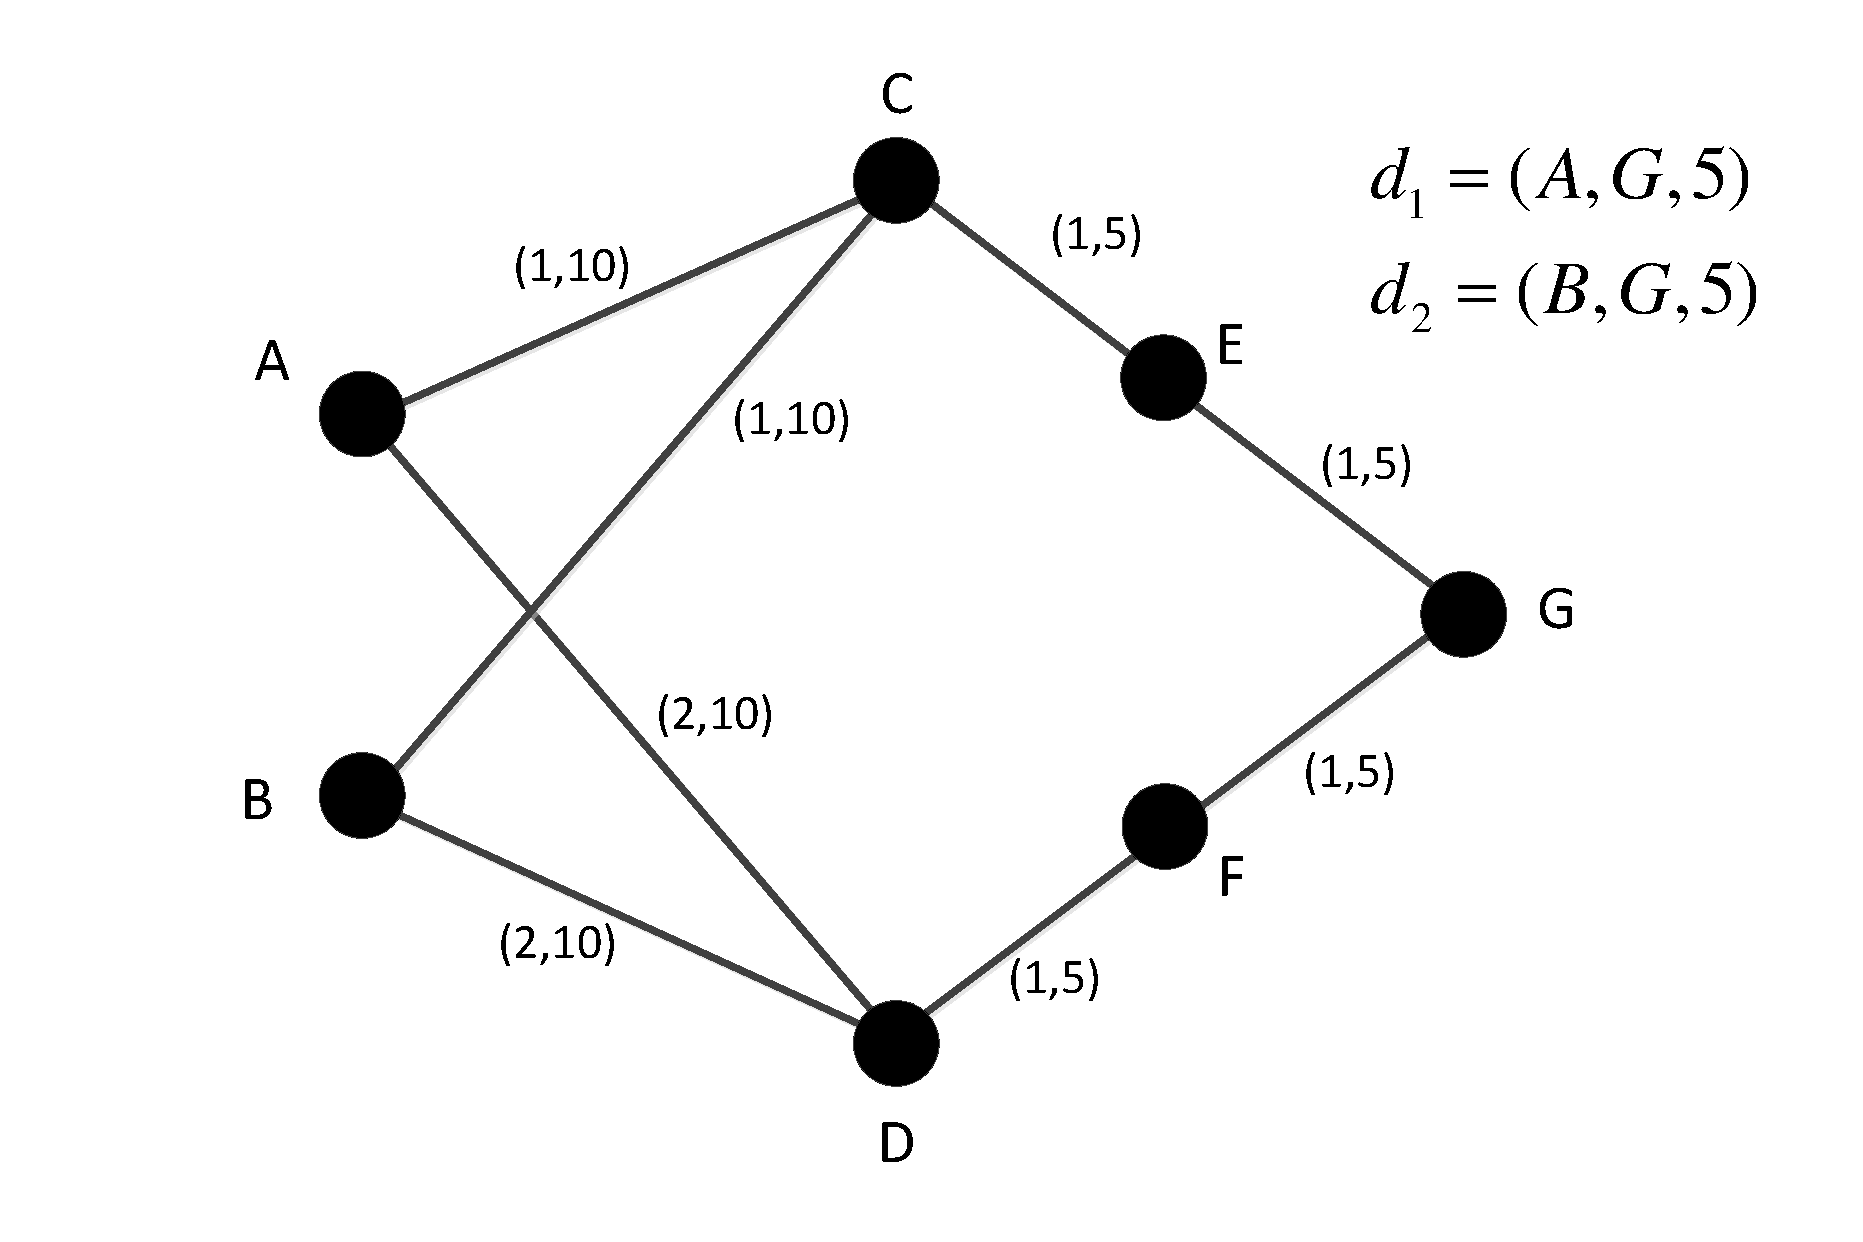
\includegraphics[width=0.4 \textwidth]{figures/random.pdf}}
    \end{center}
  \caption{{\footnotesize{链路更新例子2}}}
  \label{u1}
\end{figure}
  如上图所示,假设有存在两个业务$d_1$和$d_2$,其中$d_1$的源节点为$A$,目的节点为$G$, 其流量大小为$5$;$d_2$ 的源节点为$B$, 目的节点为$G$,其流量大小为$5$,开始时两个都分别贪心计算最短路径,$d_1$ 选择路径$A-C-E-G$,$d_2$选择路径$B-C-E-G$, 这样的话,链路$C-E$和$E-G$出现拥塞,表()展示了这个迭代过程,图()中最优的选择是让其中一个业务经过边$C-E-G$进行中继,另一个业务经过边$D-F-G$进行中继。但是的迭代过程始终无法使得两条链路发生分离,图中的链路权重始终无法达到最优条件,这是因为算法的权重迭代增加粒度太大,由于链路$C-E-G$和链路$D-F-G$每次超限都会为路径的总权重增加2个单位,假设每次迭代时链路$C-E-G$和链路$D-F-G$ 每次迭代时一共只贡献1个单位的权重增加,那么算法只需要一次迭代就能达到最优条件,此时链路$C-E-G$由于超限,权重一共增加1个单位,那么路径$A-C-E-G$ 和路径$A-D-F-G$ 权重相等都为4,同样,路径$B-C-E-G$和路径$B-D-F-G$的权重也相等了,这样两个业务才会分离开(比如业务$d_1$选择链路$A-C-E-G$, 业务$d_2$选择链路$B-D-F-G$)。但是在算法设计时,我们难以分辨哪些链路的组合会引起业务出现这种徘徊情况,为了解决链路增加粒度过大的情况,在本设计中我们采用随机选择执行更新的策略,也就是对一条流量超过容量约束的边$(i,j)$,我们以概率$\phi$ 来对他进行权重更新,每条边的权重增加粒度依然为1个单位,假设$\phi=0.5$,这种方法在一定概率上保证图()中的例子可以在一次迭代中收敛。实际实验中发现这种更新策略能够保证算法得到较优解的同时,保证收敛速度较快。
\begin{table}[t]
\newcommand{\tabincell}[2]{\begin{tabular}{@{}#1@{}}#2\end{tabular}}
\setlength{\abovecaptionskip}{0.2cm}
  \centering
 \scriptsize{
 \renewcommand{\tabcolsep}{0.09cm}
 \renewcommand{\arraystretch}{1.2}
    \begin{tabular}{| c | c | c |}
    \hline
     Iteration number & \tabincell{l}{Calculated paths for \\the two demands} & Path weights
\\ \hline
0 & \tabincell{l}{A-C-E-G \\ B-C-E-G} & \tabincell{l}{3(1+1+1) \\ 3(1+1+1)}   \\ \hline
1 & \tabincell{l}{A-D-F-G \\ B-D-F-G } & \tabincell{l}{3(2+1+1) \\ 3(2+1+1)}   \\ \hline
2 & \tabincell{l}{A-C-E-G \\ B-C-E-G} & \tabincell{l}{3(1+2+2) \\ 3(1+2+2)} \\ \hline
3 & \tabincell{l}{A-D-F-G\\ B-D-F-G} & \tabincell{l}{3(2+2+2) \\ 3(2+2+2)} \\ \hline
4 & \tabincell{l}{A-C-E-G \\ B-C-E-G} & \tabincell{l}{3(1+3+3) \\ 3(1+3+3)} \\ \hline
5 & \tabincell{l}{A-D-F-G \\ B-D-F-G} & \tabincell{l}{3(2+3+3) \\ 3(2+3+3)}\\ \hline
6 & \tabincell{l}{ ...\\ ...} & \tabincell{l}{... \\ ...}\\ \hline
\end{tabular}
 \vskip 0.2 cm
  \caption{拉格朗日更新过程(2)}
  \label{Iterprocess2}
}
\end{table}
\subsection{路径调整}
  注意到,在最优的权重代价下(最优拉格朗日乘子),LR-PROA求解到的路径集合解对于拉格朗日对偶问题的优化解(eq),但是他不一定是原来路由优化问题的优化可行解(Eqs)。作为一个例子,考察图()中的情况,图中的元组中数字分别表示链路的代价和链路上的剩余容量大小,我们假设有两个业务需求$d_1$和$d_2$,其中两个业务的流量需求都是1个单位,假设在某一个迭代过程中,LR-PROA 为两个业务算出来的链路都是$A-C-E-D$, 这条路径选择是对偶问题的最优解,但是他对于原问题来说是不可行的解,因为链路$(C,E)$ 上承载的链路容量大于了链路$(C,E)$ 上的容量。所以,为了寻找原问题的最优解,LR-PROA会继续迭代,这是由于每个业务在选择路径的时候没有去考虑其他业务所选择的路径,但是我们容易看到这个例子中所有路径权重都一样(都等于3),也就是说,图中存在着大量的等价链路,但是在这个例子中两个业务恰好都选择了冲突的那一条路径$A-C-E-D$,如果业务$d_1$ 的路径被调整到$A-D$,业务$d_2$的链路被调整到$B-F$, 那么,我们可以得到原问题的最优可行解,所以通过这里的启发,我们发现需要设计一种业务路径调整算法来主动避免链路出现冲突,从而减小算法的迭代次数,得到原问题的优化的可行解。
\begin{figure}
\setlength{\belowcaptionskip}{-0.1cm}
  \begin{center}
    {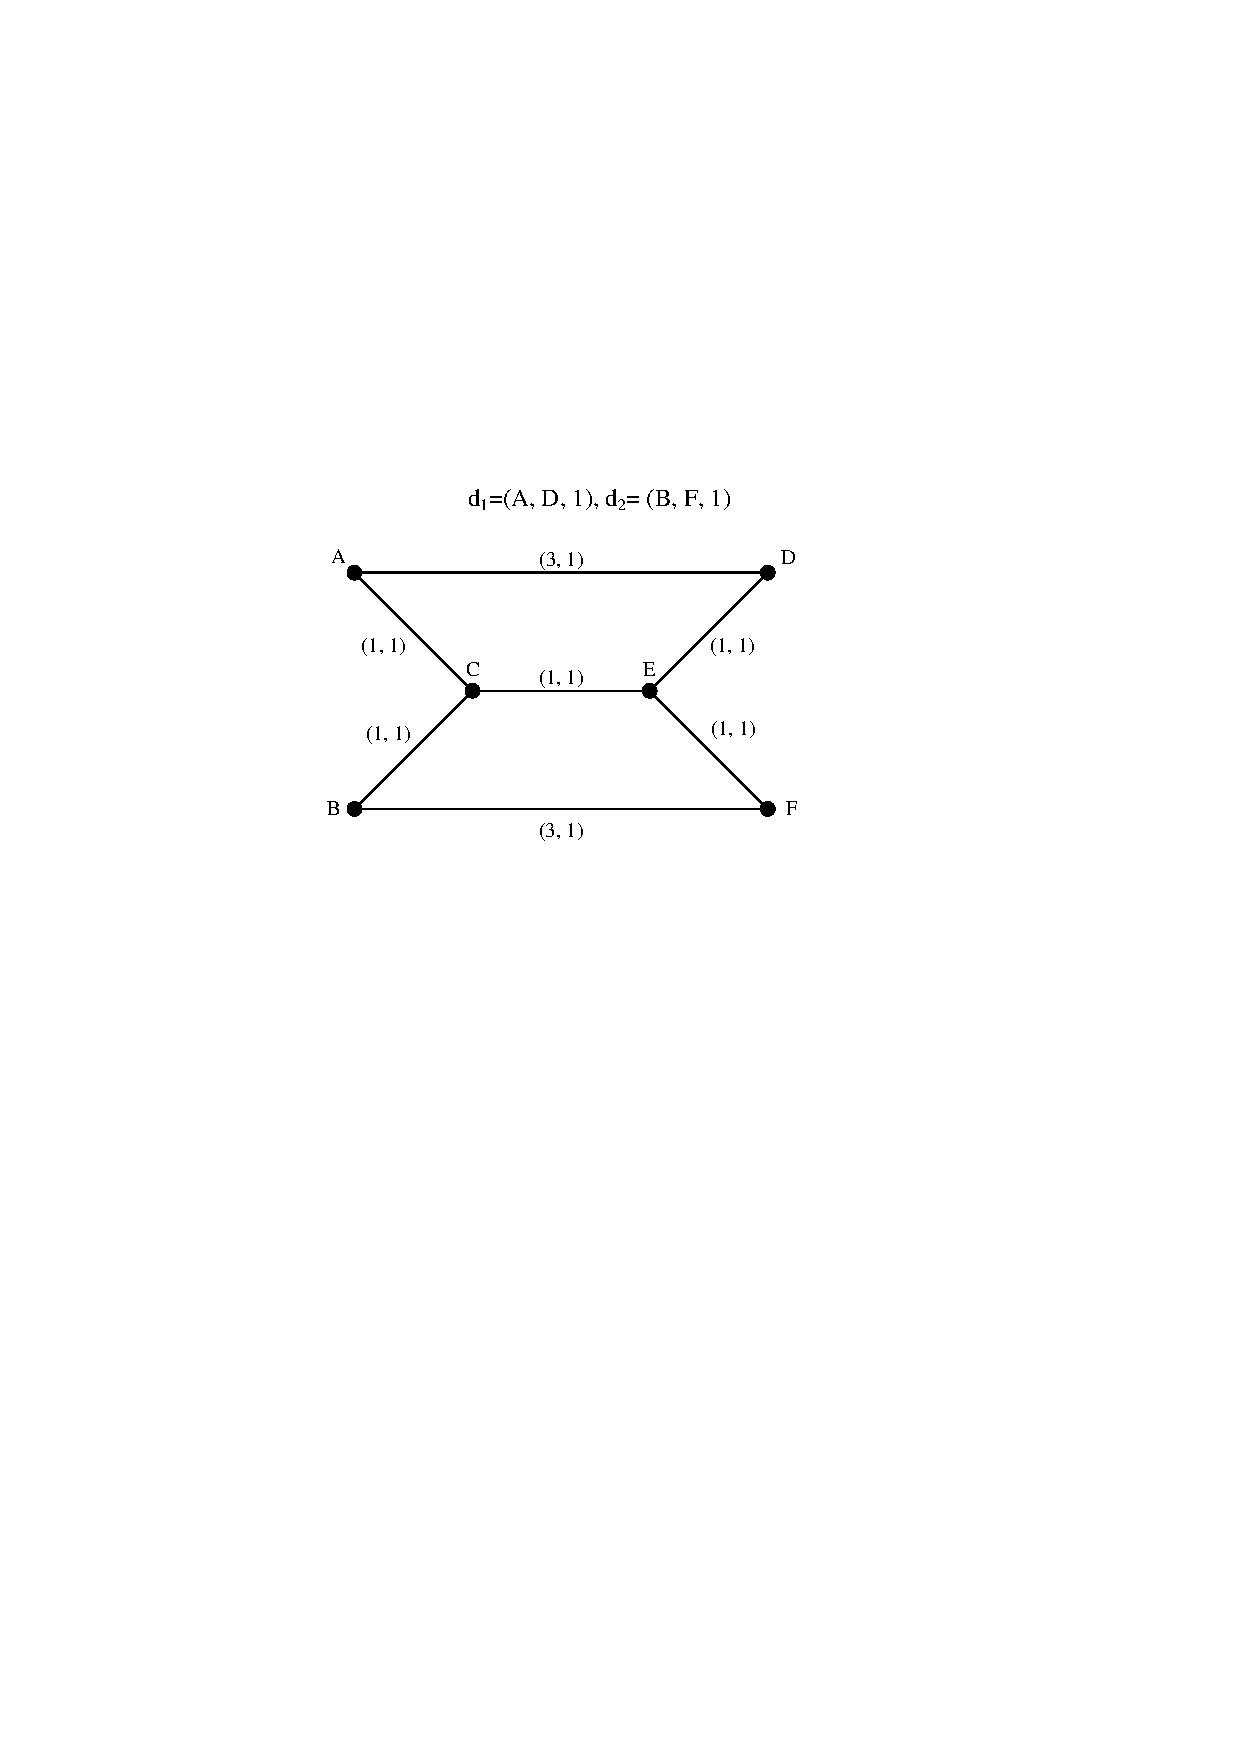
\includegraphics[width=0.4 \textwidth]{figures/PathAdj.pdf}}
    \end{center}
  \caption{{\footnotesize{路径调整例子}}}
  \label{IterNum}
\end{figure}

为了说明业务路径调整算法,我们引入一些符号,假设$P$表示步骤2所计算出来的路径集合,其中$p_d\in P$ 表示业务$d$ 的路径, $rp_{d}$ 表示路径$p_d$上的可用带宽,$rp_{d} = min\{r_e | e\in p_d\}$,其中$r_e$ 表示链路$e$上的剩余带宽,$D_l$ 表示剩余业务集合,表示这些业务不能在不违背容量约束的情况下被加入网络中。
\begin{algorithm}[t]
\begin{algorithmic}[1]
\caption{{Path Adjustment}}
\label{PathAdj}
\Require
网络拓扑 $G(V, E)$;
业务量需求集合 $D$;
步骤2算出来的路径集合 $P_{in}$;
\Ensure
调整后的路径集合 $AP$;
\State {把业务按照值$\frac{bw_d}{\sqrt{|p_d|}}$进行降序排序}
\For{each traffic demand $d \in D$}
\If{$rp_{d} \ge  bw_d$ }
\State{把路径 $p_d$加入到$AP$中}
\State{在图G(V,E)中更新路径$p_d$所经过链路的剩余带宽}
\Else
\State {把业务$d$加入到剩余集合$D_l$中}
\EndIf
\EndFor
\State{$G^{'}(V^{'},E^{'})=G(V,E)$}
\For{each traffic demand $d \in D_l$}
\State{$G^{''}(V^{''},E^{''})=G^{'}(V^{'},E^{'}$}
\For{each link $e \in E^{'}$}
\If{链路$e的剩余容量< bw_d$}
\State{把链路 $e$ 从图$G^{''}(V^{''},E^{''})$中移除}
\EndIf
\EndFor
\State{在图$G^{''}(V^{''},E^{''})$中为业务$d$计算最短路径$p$(链路代价都设为1)}
\If{$\frac{|p|}{|p_d|}\le \delta$}
  \State{把路径 $p$ 加入到 $AP$,并把业务从集合$D_l$中移除}
  \State{在图$G^{'}(V^{'},E^{'})$中更新路径$p$所经过链路的剩余带宽}
  \State{$G(V, E)=G^{'}(V^{'},E^{'})$}
\EndIf
\EndFor
\Return {$AP$}
\end{algorithmic}
\end{algorithm}

路径调整算法的主要思想是通过调整一小部分业务的路径来得到原问题的优化可行解,算法首先对业务进行排序,这里采用上一节() 类似的思想对业务进行排序,一方面,要使得目标函数变小,那些流量需求较大的业务应该优先被加入到网络中,但是如果大流量的业务的路由代价很大,经过了一条很长的路径,就会大量的浪费网络中的链路容量资源,所以算法过程对当前染色体$j$中的业务和其路径按照$\frac{bw_d}{\sqrt{|p^{k^d_j}_d|}}$的值进行排序,其中${bw_d}$代表当前业务$d$ 所需要的流量大小,$|p^{k^d_j}_d|$ 代表当前染色体$j$ 所选择的$p^j_d$中的第${k^d_j}$条路径的代价大小,这样按照顺序试图将业务加入到网络中,如果$rp^{k^d_j}_d>=bw_d$,表示业务可以被加入到网络中,那么加入此业务并且更新网络链路的剩余容量值,反之,如果$rp^{k^d_j}_d<bw_d$,则表示业务选择的路径上有链路容量不足以承载此业务,那么将业务加入剩余集合$D_l$ 中,循环结束后,得到一个剩余网络,根据前面的讨论,在剩余网络中可能存在一些等价路径,所以剩余链路中依然有很多可用资源,而且观察目标函数,发现算法需要优先保证网络中加入更多的业务,所以算法重新在剩余网络中为剩余业务计算路径,算法依次遍历集合$D_l$, 看能否在剩余网络中为业务寻找一条路径,首先剔除那些链路剩余容量小于业务流量$bw_d$ 的链路,这样保证求出来的路径肯定是满足容量约束的,由于剩余链路是残余网络,所以可能会求出跳数很长的路径,如果跳数太长了,会占用太多的资源,不能达到优化的目的,所以算法设置一个跳数阈值$\delta$来进行约束,如果求出来的路径跳数大于$\delta$则认为路径不合法。如果路径跳数小于$\delta$ 则加入业务到网络中,并更新网络链路容量。虽然这个过程是串行的,但是这个过程是很快速的,这主要有以下三个原因 第一,由于剩余网络中大量存在链路容量不足,能参与计算的链路很少,对一个剩余业务$d$,在计算路径之前,算法会剔除那些剩余容量小于$bw_d$ 链路,所以实际上参与计算的网络拓扑很小;第二,这个时候计算最短路径不用考虑链路代价,直接使用BFS 进行计算。第三,剩余业务量集合$D_l$ 本身较小,算法越往后面加入业务,可用链路会越来越小,网络会进一步变小。通过这个路径调整算法,可以得到原问题的一个优化可行解,这个解作为当前迭代产生的最优解,和全局最优解进行比较,如果这个解优与全局最优解则更新全局最优解,进入下一次迭代。
\subsection{仿真实验分析}
\subsubsection {仿真介绍}
为了证明LR-PROA和GA-PROA的优化效果,我们把两个算法的优化结果和基于备选路径的MILP模型[] 的最优目标值进行比较,其中每个业务的备选路径数量为10条,我们使用CPLEX 来求解MILP 模型,由于CPlex求解MILP需要很大的计算量,对于大规模的网络,我们无法得到MILP的最优值,因此我们设置了10 分钟的求解时间限制,当Cplex求解时间超过10分钟后,我们停止求解过程,记录求得Cplex 求解的最优可行目标函数,以及MILP模型的最优值得下界。
为了观察LR-PROA和GA-PROA的加速效果,我们分别设计两个算法串行版本LR-PROA和GA-PROA,并把LR-PROA和GA-PROA 与LR-PROA 和GA-PROA进行比较,其中LR-PROA中的路由算法采用带堆优化的dijkstra 算法,dijkstra算法的复杂度为($|N|\lg |N| +|E|$), 为了体现LR-PROA的加速效果,本文还对串行的dijkstra进行了进一步的优化,讨论如下:假设一批业务$D$ 的源节点相同,这一批业务的目的节点组成集合$D$,那么我们在求解dijkstra 算法时,当最小堆吐出了$D$ 中的所有点之后,我们就提前结束了dijkstra,所以当集合$D$ 比较小时,实际的算法复杂度一般是远远小于($|N|\lg |N| +|E|$) 的。

我们分别采用ERdos-R enyi (ER) [] and Barab asi-Albert (BA) []两种模型来生成实验网络拓扑,实验中的网络拓扑中点的平均度数为6。 我们分别比较算法的目标函数,加速效果和算法的收敛性质,LR-PROA和LR-SROA中的$\delta$和$K$被分别设置为10 和30。GA-PROA与LR-PROA 都是通过CUDA 8.0 进行设计,跑算法的服务器配置有四个Intel Xeon E5-2630 CPU 和一个 NVIDIA Tesla K40M GPU。
 \subsubsection{目标函数比较}
 图12和图15分别显示了在点数为200和1000的网络中,目标函数随着业务数量规模变化的折线图,图中的网络链路容量大小为100,业务的流量需求大小为$[1,100]$的均匀随机值。从图中我们可以看到目标函数大致随着业务数量呈现线性增加,这和目标函数的表达式相吻合。从图中可以看到LR-SROA/LR-PORA的算法优化目标明显优于遗传算法LR-PROA/LR-SROA,这是因为:1. 遗传算法提前陷入了局部最优解,导致算法提前结束。2.遗传算法是基于备选路径的,所以其没有LR-SPOA/LR-PROA 那么灵活, LR-SPOA/LR-PROA 会动态的寻找业务的路径,根据网络链路的动态状况重新求解路径,从而充分利用网络链路资源,从而减小目标函数。

和MILP的Cplex解相比,在小网络(点为200)中,由于Cplex的计算压力不大,其计算出来的解略微优于LR-SPOA/LR-PROA。
 可以看到图中MILP-bound和LR-SPOA/LR-PROA差距很小,这说明在小网络下,LR-SPOA/LR-PROA 算法求出的解已经很接近MILP 的理论最优解了;在大网络中(点数为1000,图**),由于Cplex的计算压力增大,LR-SPOA/LR-PROA的解已经优于Cplex 的解。比较MILP-bound 我们可以发现LR-SPOA/LR-PROA的解离MILP-bound 有一定差距,这是可能有两个原因:1.Cplex的计算压力大,导致求得的bound可能不够精确。2.LR-SPOA/LR-PROA陷入了局部最优解。
图15和图17表示在容量变化下的目标函数值变化,其中业务数量为点数的6倍,网络链路容量从100到250变化。随着容量的增加目标函数大致呈现线性下降,这是因为链路容量增加后,网络资源增大,网络可容纳的业务增加,业务可选择的优化路径增增多,业务的路径代价下降,阻塞的大量减少,所以目标函数呈现大幅下降。
\begin{figure}
\setlength{\belowcaptionskip}{-0.1cm}
  \begin{center}
    {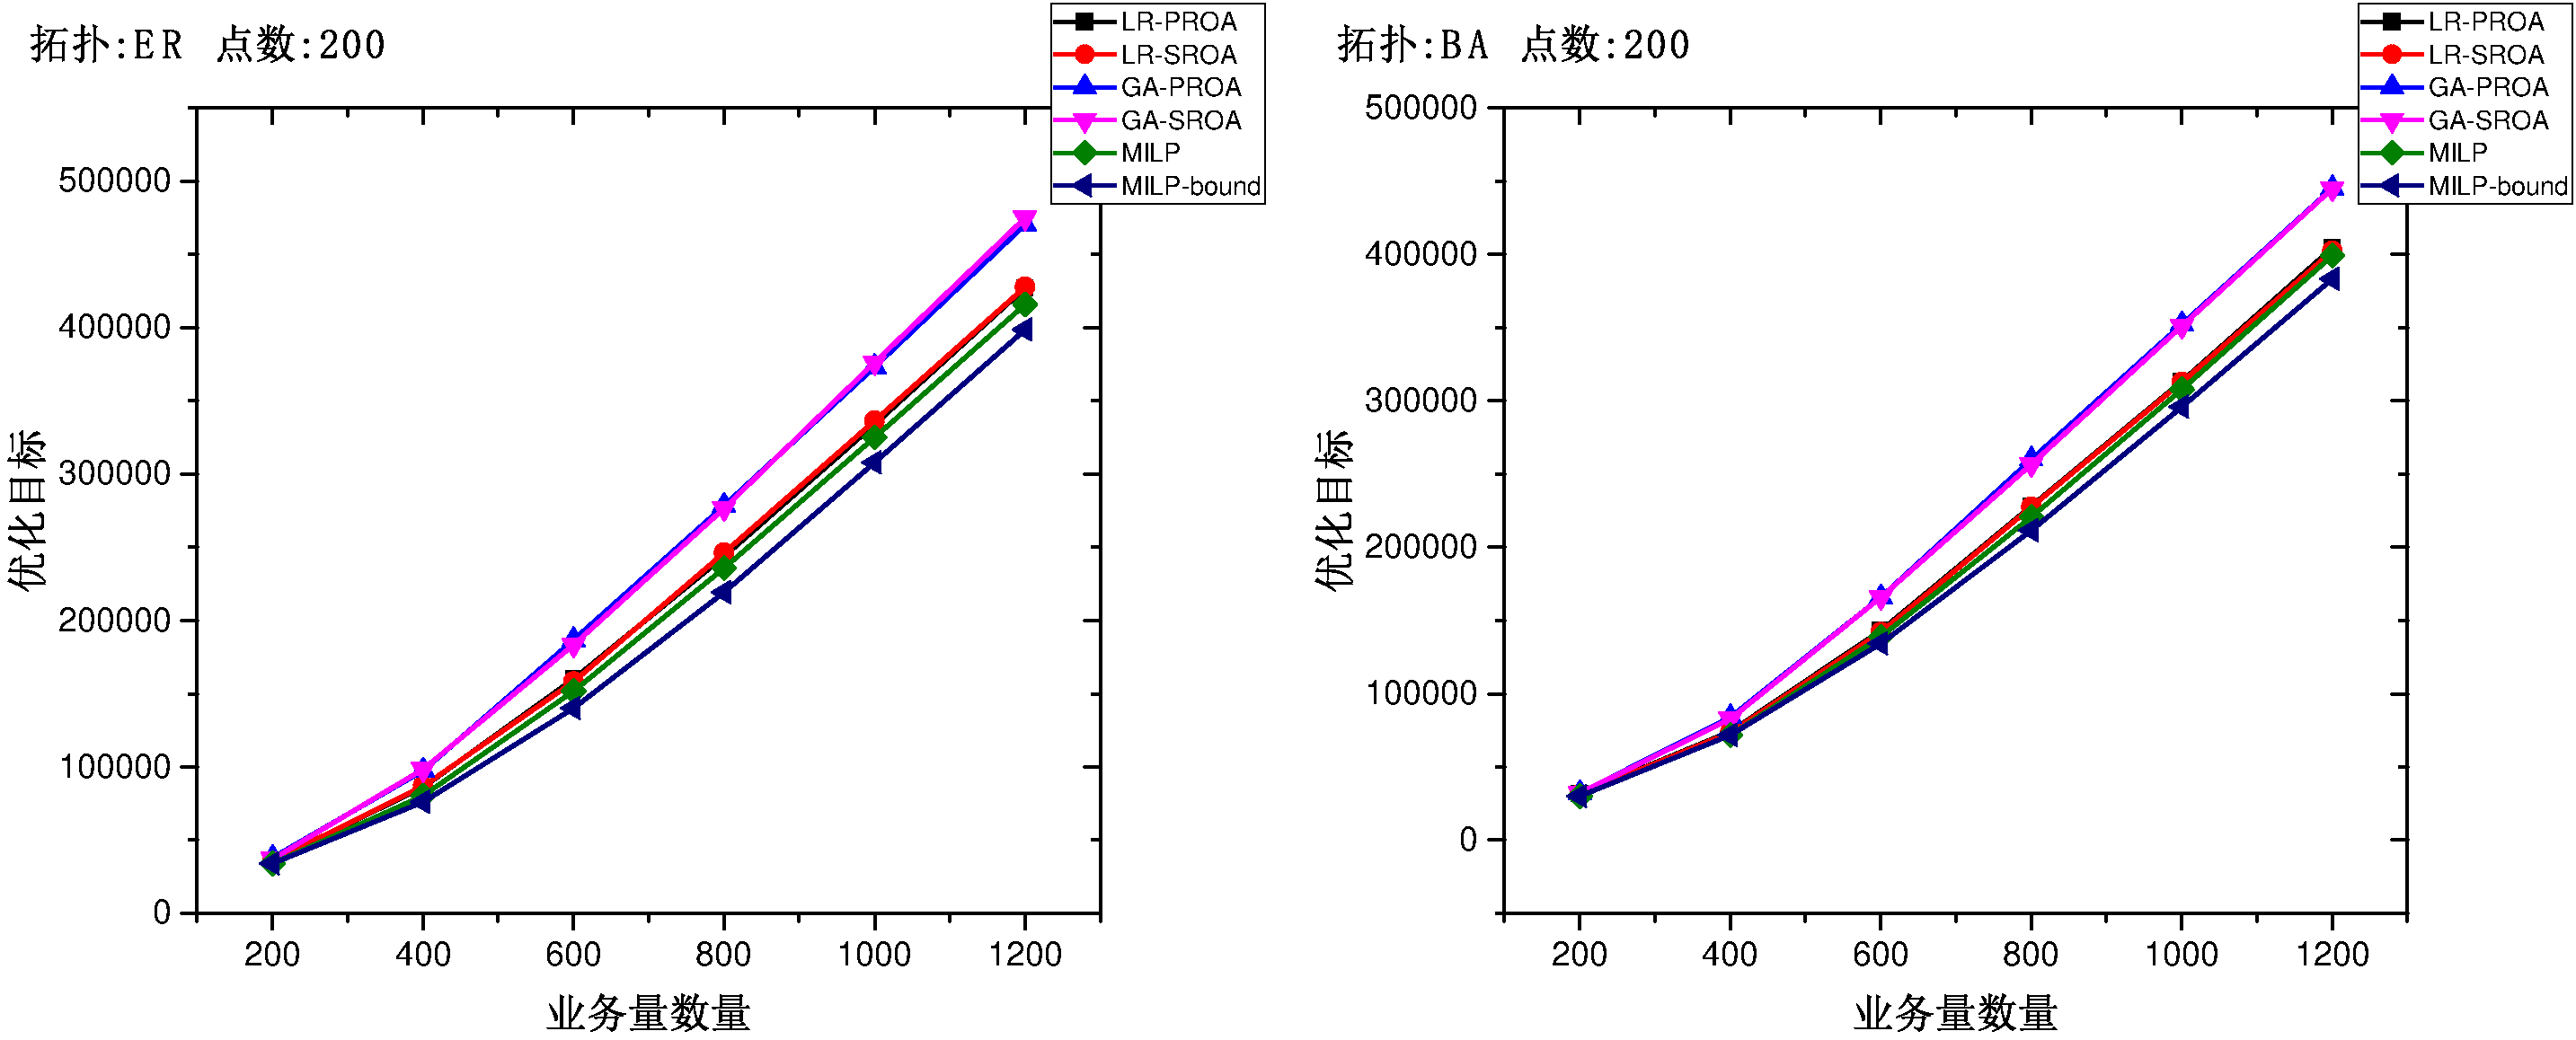
\includegraphics[width=1 \textwidth]{figures/OB-TA-200.pdf}}
    \end{center}
  \caption{{\footnotesize{objective-task}}}
  \label{obt200}
\end{figure}
 \begin{figure}
\setlength{\belowcaptionskip}{-0.1cm}
  \begin{center}
    {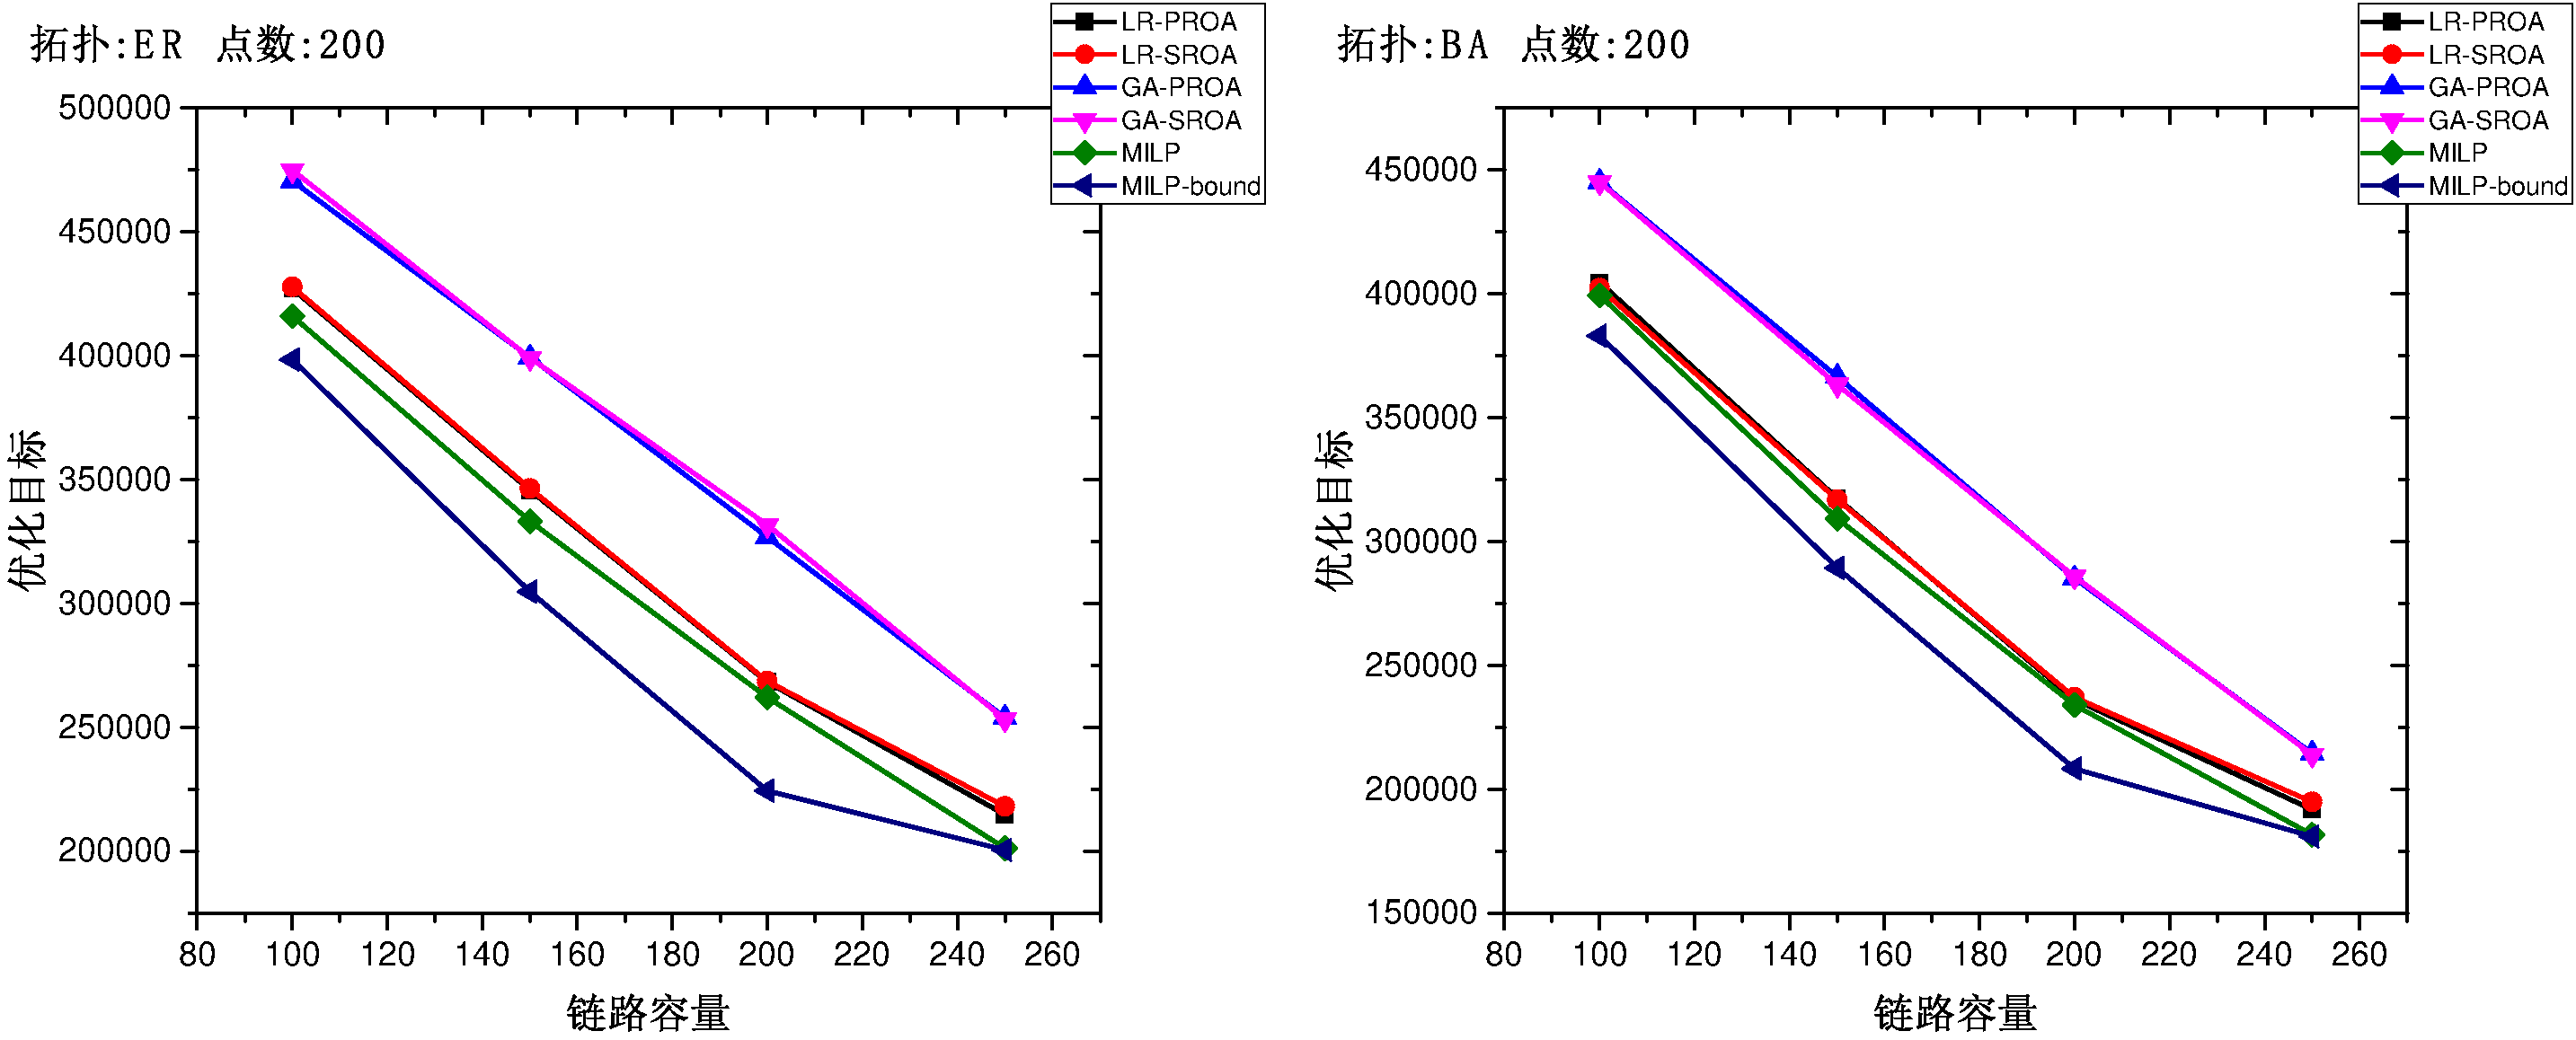
\includegraphics[width=1 \textwidth]{figures/OB-CA-200.pdf}}
    \end{center}
  \caption{{\footnotesize{objective-task}}}
  \label{IterNum}
\end{figure}
 \begin{figure}
\setlength{\belowcaptionskip}{-0.1cm}
  \begin{center}
    {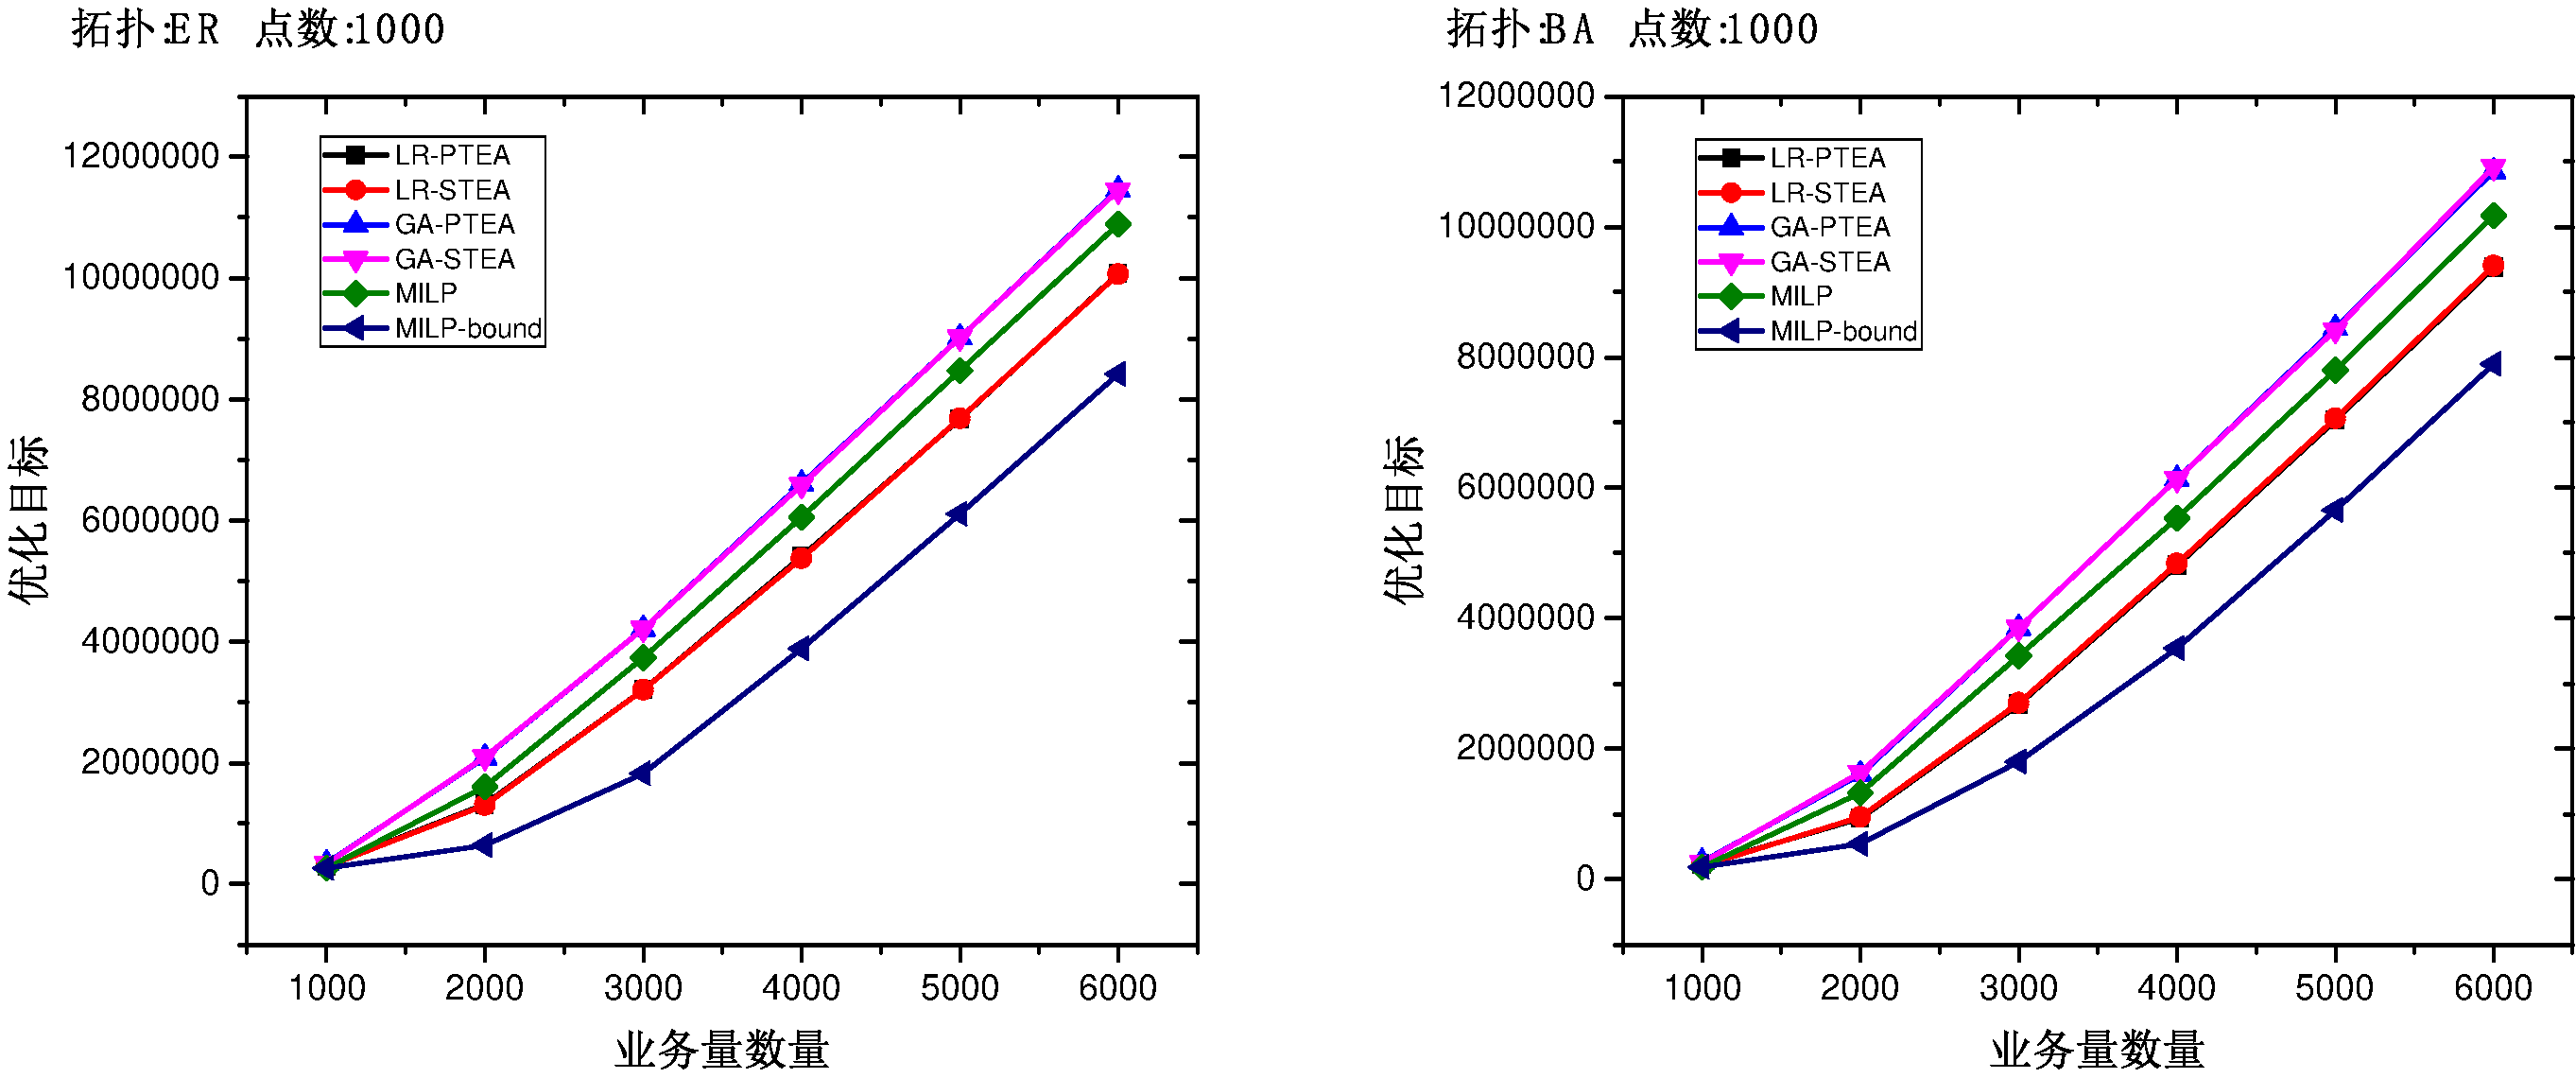
\includegraphics[width=1  \textwidth]{figures/OB-TA.pdf}}
    \end{center}
  \caption{{\footnotesize{objective-task}}}
  \label{IterNum}
\end{figure}
  \begin{figure}
\setlength{\belowcaptionskip}{-0.1cm}
  \begin{center}
    {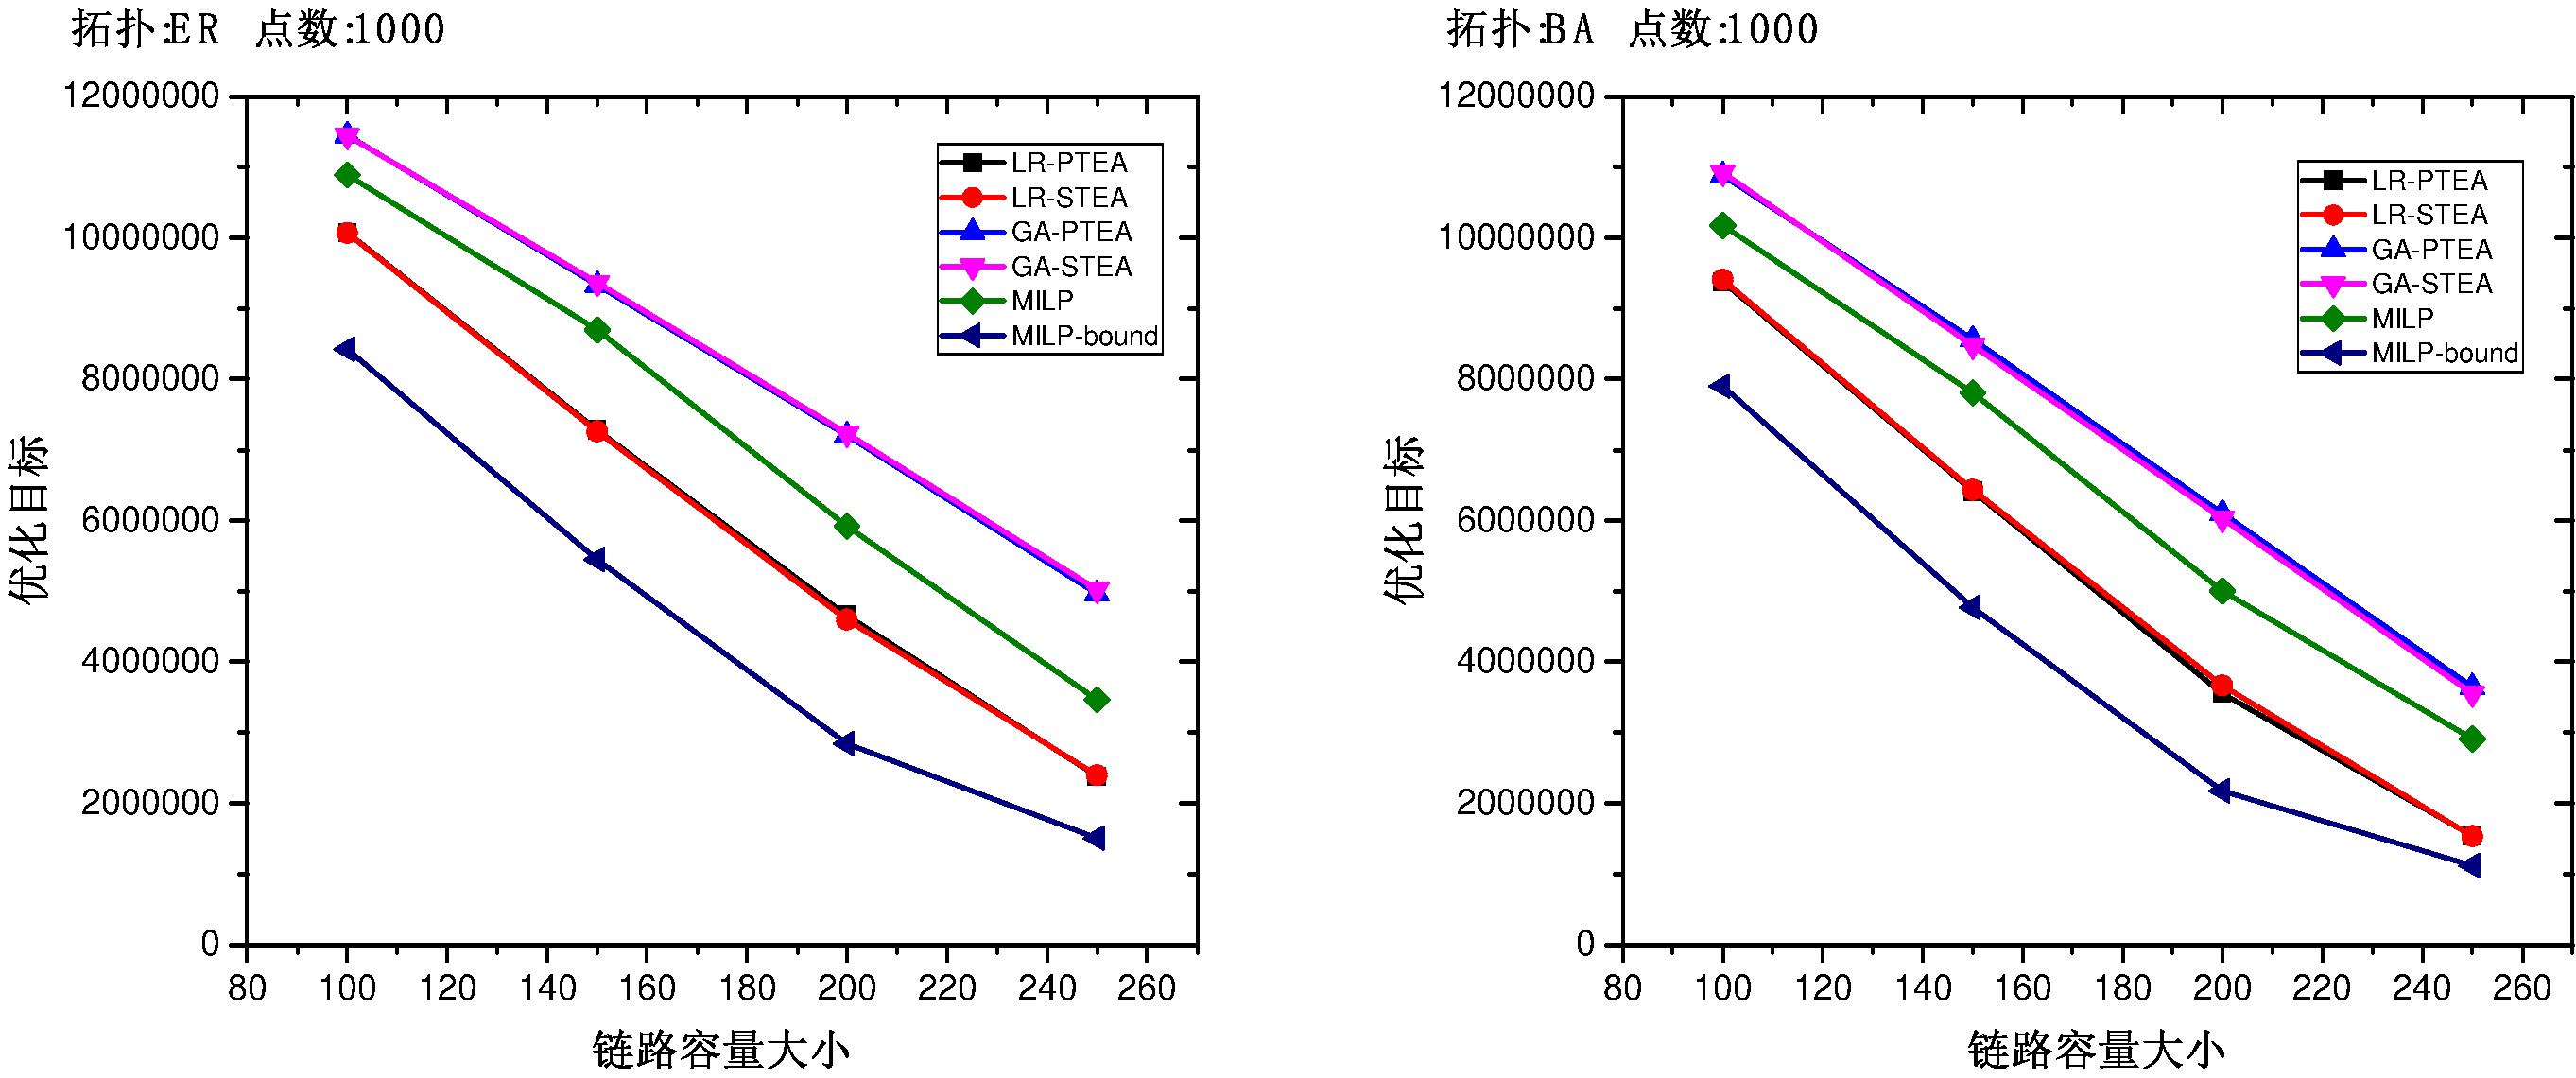
\includegraphics[width=1 \textwidth]{figures/OB-CA.pdf}}
    \end{center}
  \caption{{\footnotesize{objective-task}}}
  \label{IterNum}
\end{figure}
\subsubsection{算法时间比较}
  图18和图19分别列出了算法在BA和ER拓扑下的计算时间随着业务数量增加的变化情况,图中拓扑节点数量为1000,业务数量从1000 到6000变化,业务流量为1到100的均匀随机值,链路的容量为100。由于各种算法的时间差距过大,我们用三种不同的尺度进行展示。首先,CPlex的时间限制都为10分钟,所以我们不再列出来。
  图中我们可以看到GA-PROA相对于GA-SROA加速很多大约为30倍左右,但是由于遗传算法本身的缺陷,所以GA-PROA的计算时间是很糟糕的,这是因为基于备选路径的遗传算法的初始值染色体较差,所以需要大量的迭代次数才能收敛,而且遗传算法评价步骤的本身的计算量也很大。
  观察LR-SPOA和LR-PROA,发现LR-SPOA和LR-PROA的时间曲线会发生大幅度的波动,这是因为,算法的迭代次数变化较大,我们设置算法在30次后未找到更优解之后停止,其实30次设置得偏小,算法有可能会找到更好的解,但是这些解的优化程度很小(通过第**的收敛图,可以看到算法在前50次内下降幅度较大,后面的下降幅度很小),所以为了优化整体时间,我们设置迭代次数为较小的30 次,由于30 偏小,所以可能会导致算法的提前结束,从而导致算法的迭代次数变化幅度较大,从而引起整体时间上的幅度变化。
  观察图18和19,我们发现当业务数量增加到两倍点数以上后,LR-PROA相对于LR-SROA有较大加速,其中拓扑大小为1000 时,LR-PROA 相对与LR-SROA有平均6-7倍的加速。
  图20和图21表示算法时间随着网络链路容量的变化情况,其中业务数量为6倍网络的点数大小,在拓扑点数为1000的情况下,可以看到LR-PROA相对与LR-SROA有平均6-7倍的加速。
  图22和图23表示算法计算时间随着网络拓扑大小的变化情况,其中加入的业务数量为网络拓扑点数目的6倍,可以看到随着网络拓扑变大,计算时间也相应增加,GA-PROA的计算时间不管在在小拓扑还是大拓扑下都远远大于LR-PROA 的计算时间。拓扑较小时LR-PROA相对与LR-SROA的加速很小,当时随着网络的拓扑规模的增加,LR-PROA的计算时间大幅上升,而采用GPU上计算的LR-PROA 上升幅度较小,使得随着在网络拓扑达到一定规模后LR-PROA对LR-SROA有较大的加速优势,加速比随着网络拓扑大小的增大从开始的1倍变化到最后的接近9 倍,这充分体现出了GPU进行大规模计算的优势。
\begin{figure}
\setlength{\belowcaptionskip}{-0.1cm}
  \begin{center}
    {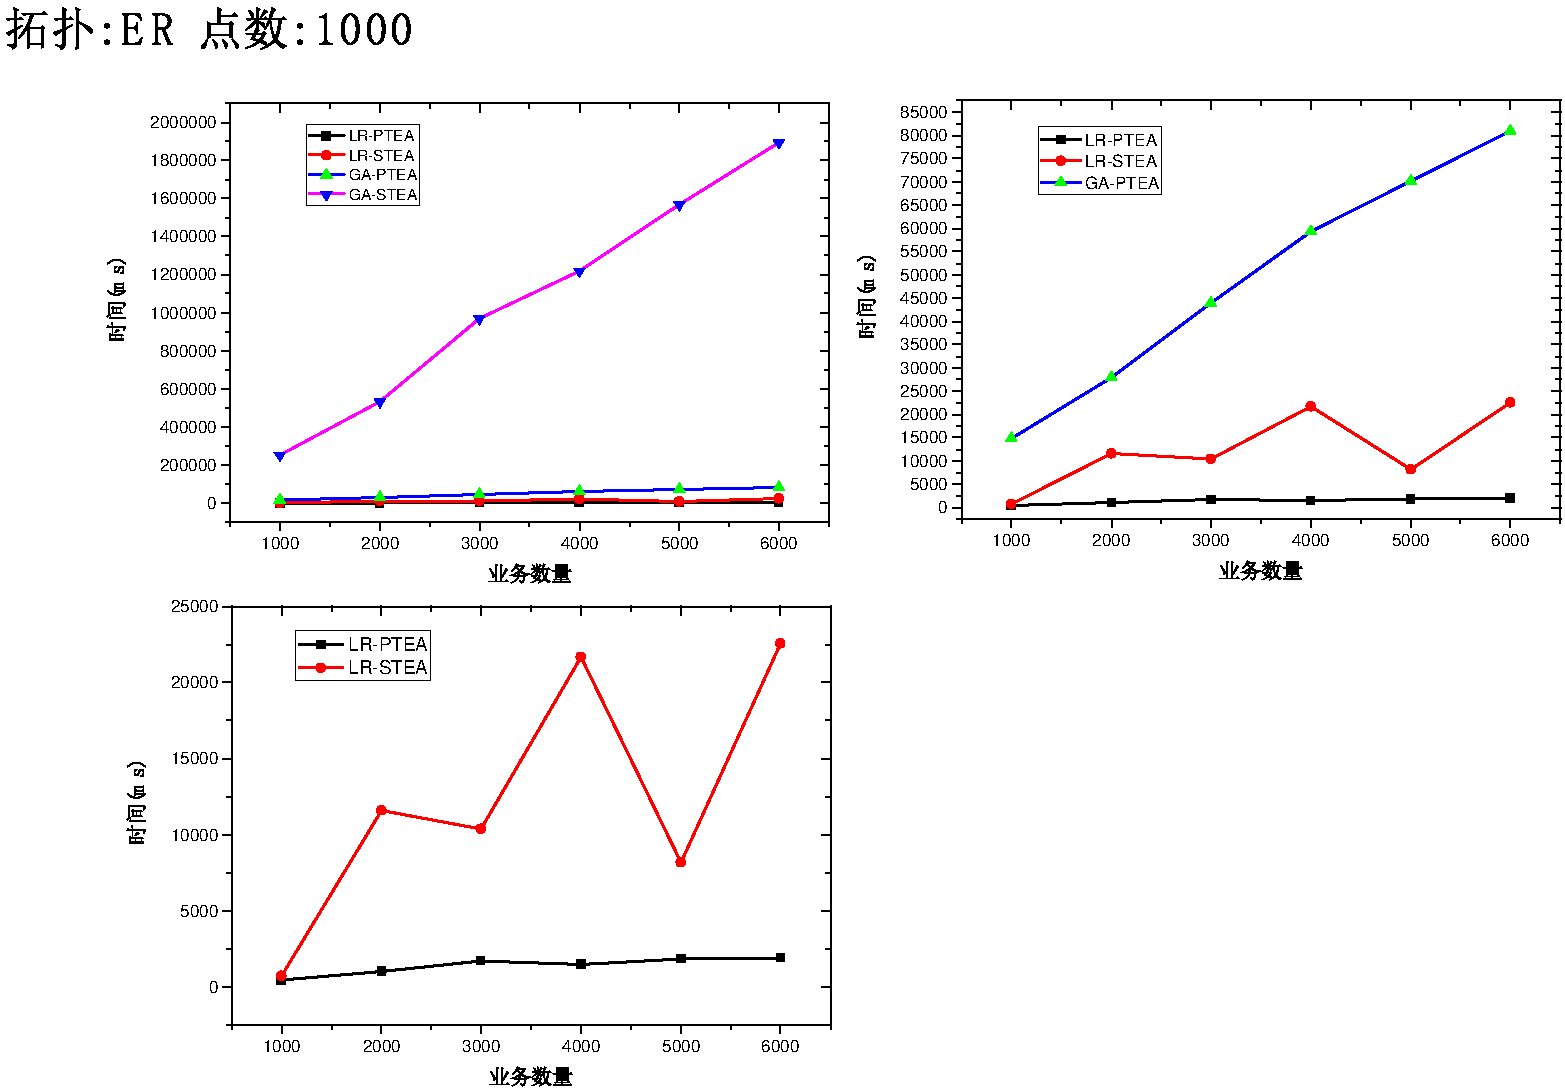
\includegraphics[width=1 \textwidth]{figures/TI-ER-TA-1000.pdf}}
    \end{center}
  \caption{{\footnotesize{objective-task}}}
  \label{IterNum}
\end{figure}
\begin{figure}
\setlength{\belowcaptionskip}{-0.1cm}
  \begin{center}
    {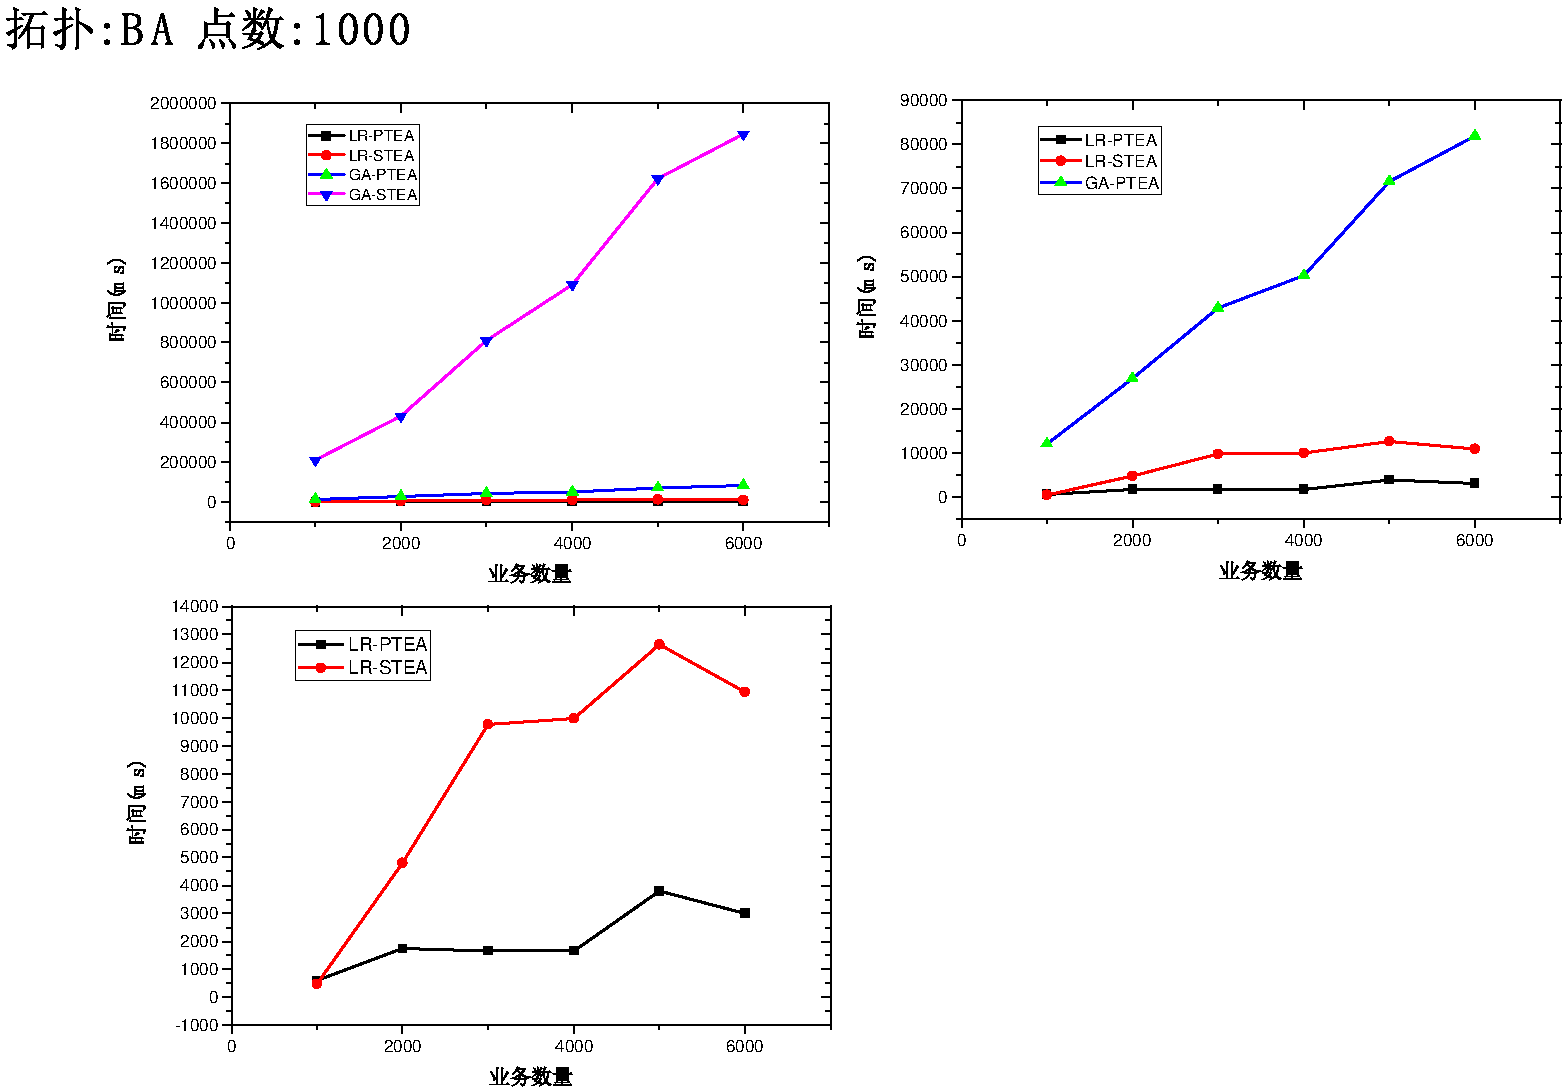
\includegraphics[width=1 \textwidth]{figures/TI-BA-TA-1000.pdf}}
    \end{center}
  \caption{{\footnotesize{objective-task}}}
  \label{IterNum}
\end{figure}
\begin{figure}
\setlength{\belowcaptionskip}{-0.1cm}
  \begin{center}
    {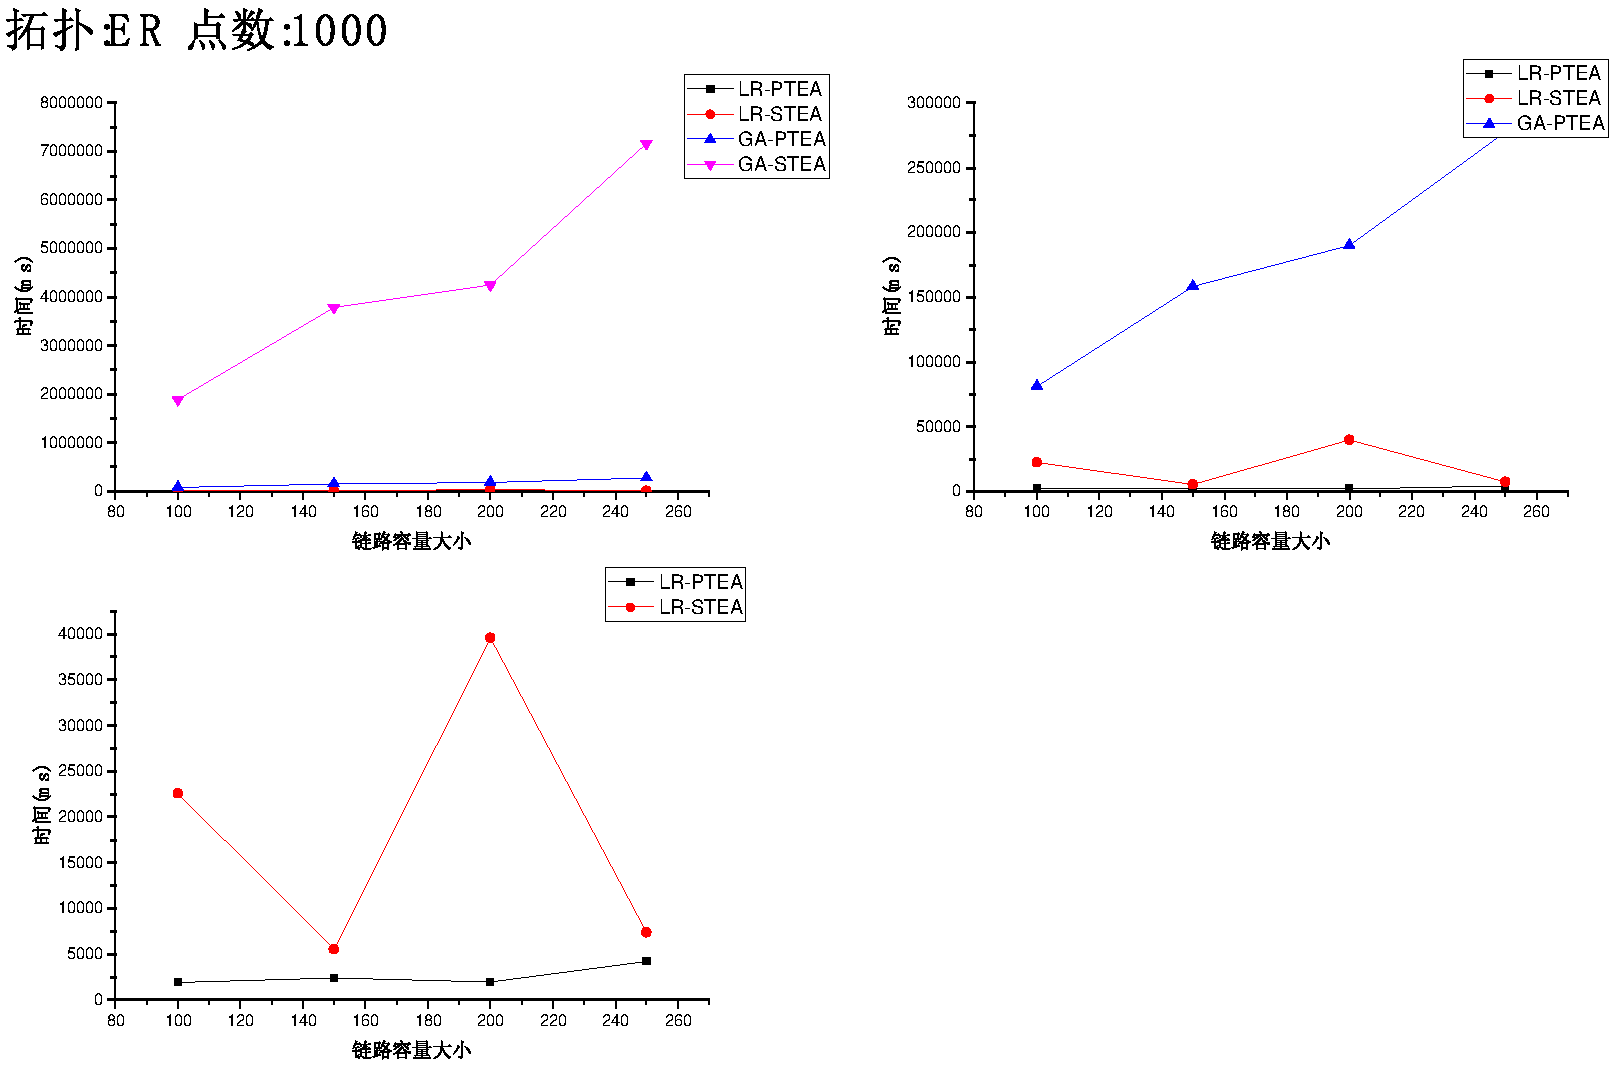
\includegraphics[width=1 \textwidth]{figures/TI-ER-CA-1000.pdf}}
    \end{center}
  \caption{{\footnotesize{objective-task}}}
  \label{IterNum}
\end{figure}
\begin{figure}
\setlength{\belowcaptionskip}{-0.1cm}
  \begin{center}
    {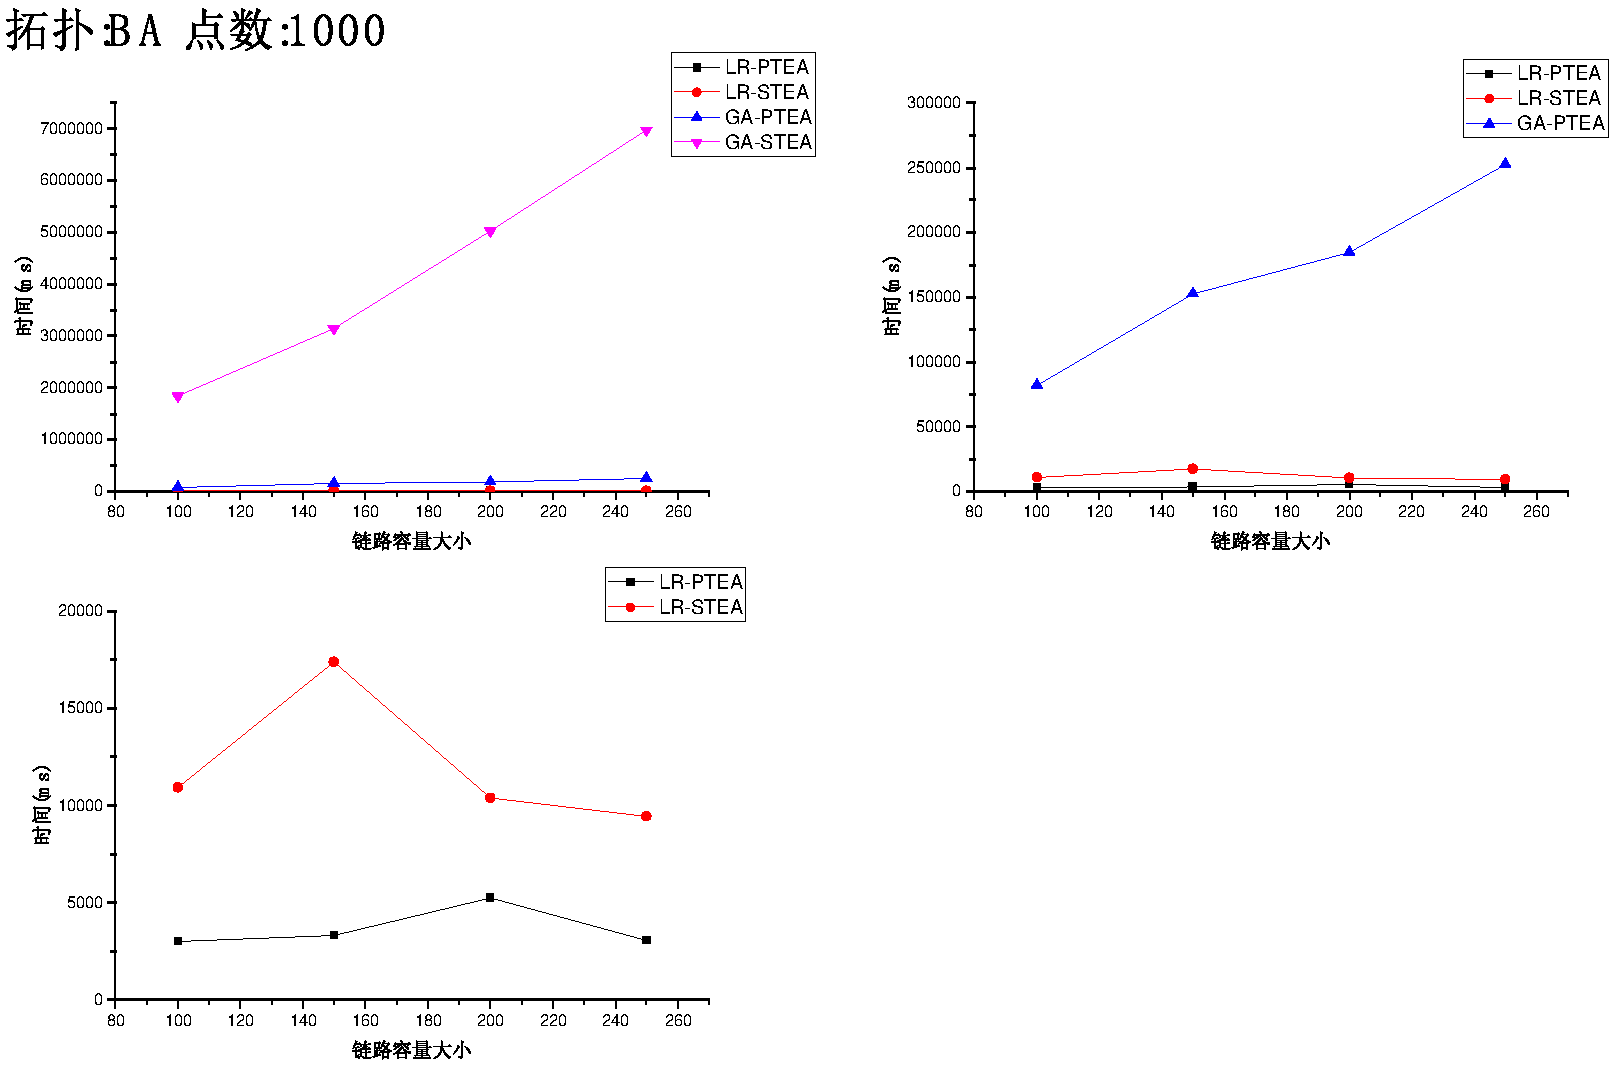
\includegraphics[width=1 \textwidth]{figures/TI-BA-CA-1000.pdf}}
    \end{center}
  \caption{{\footnotesize{objective-task}}}
  \label{IterNum}
\end{figure}
\begin{figure}
\setlength{\belowcaptionskip}{-0.1cm}
  \begin{center}
    {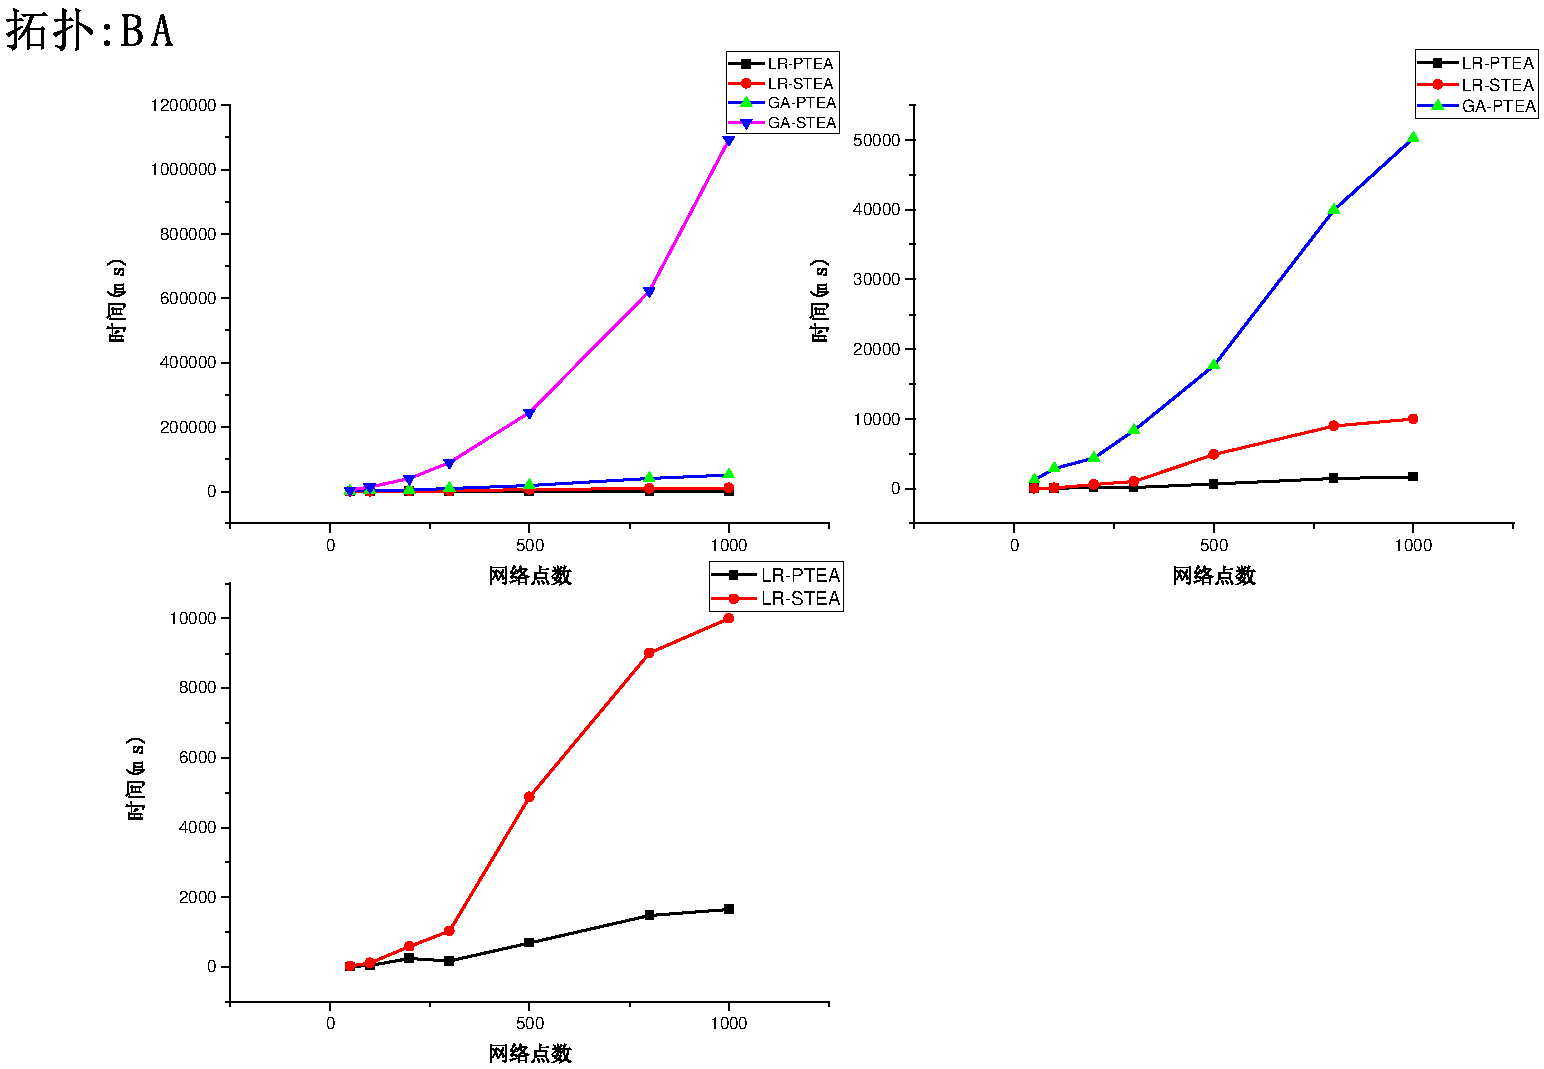
\includegraphics[width=1 \textwidth]{figures/TI-BA-NO.pdf}}
    \end{center}
  \caption{{\footnotesize{objective-task}}}
  \label{IterNum}
\end{figure}
\begin{figure}
\setlength{\belowcaptionskip}{-0.1cm}
  \begin{center}
    {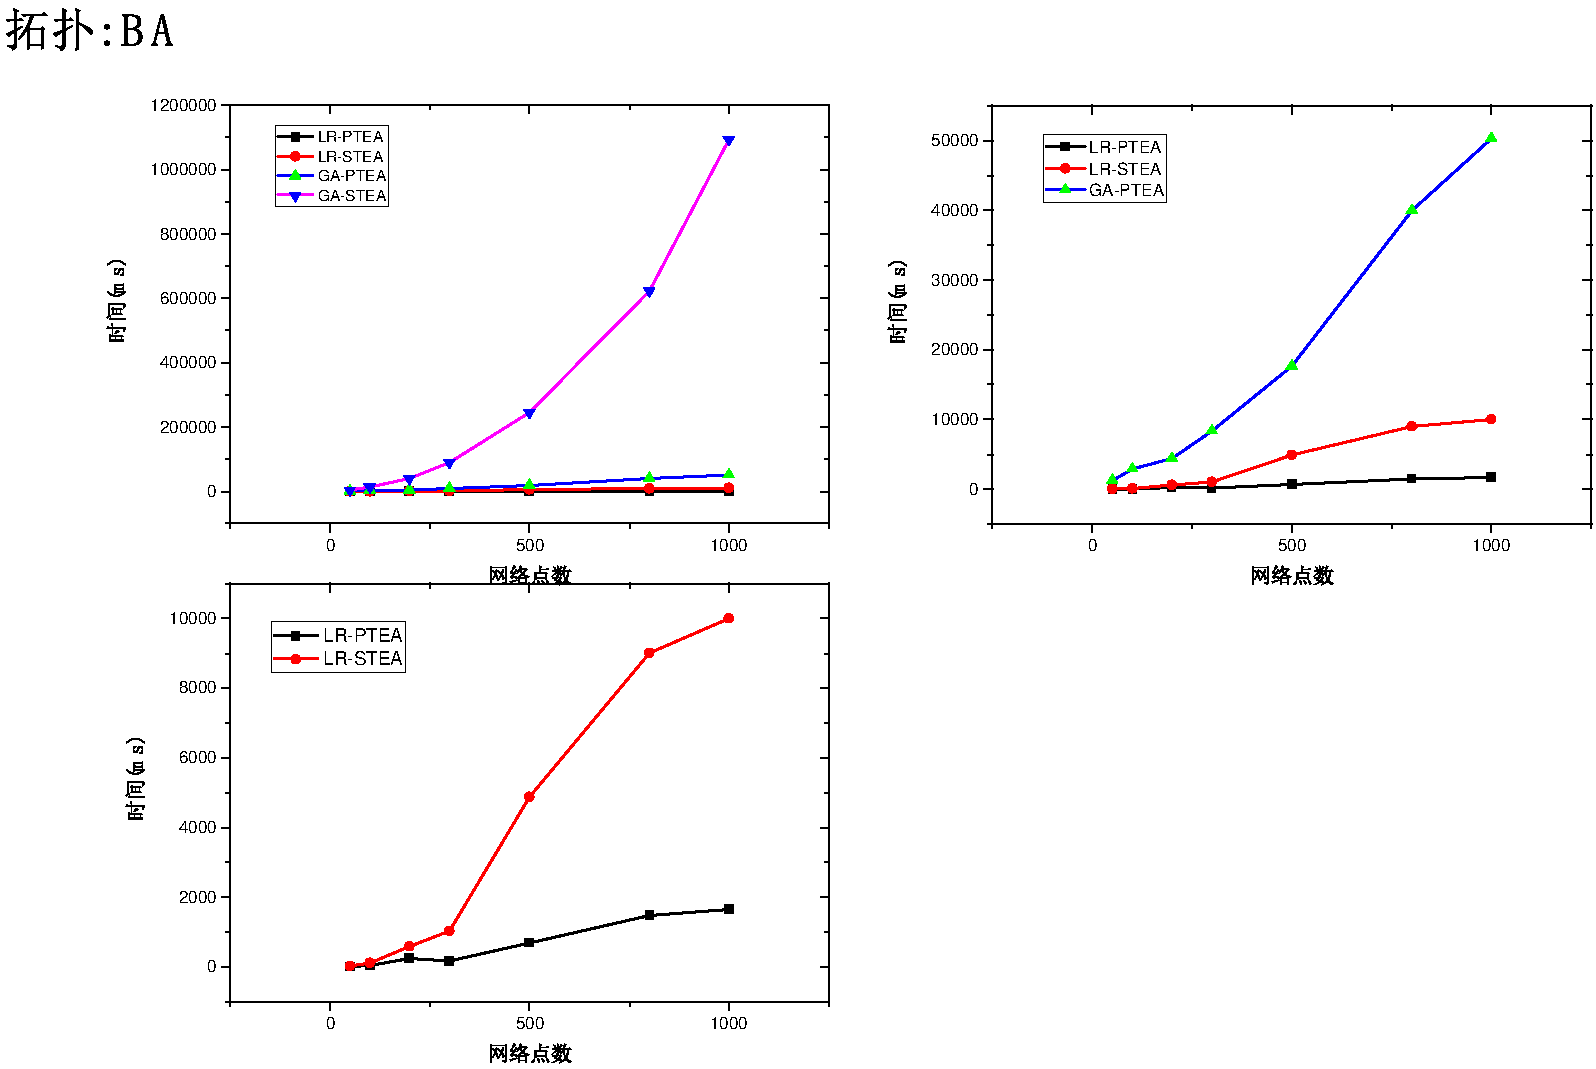
\includegraphics[width=1 \textwidth]{figures/TI-ER-NO.pdf}}
    \end{center}
  \caption{{\footnotesize{objective-task}}}
  \label{IterNum}
\end{figure}
\subsubsection{算法收敛性}
图24和图25分别是GA-PROA和LR-PROA的收敛过程图。可以看到遗传算法的初始值较差,迭代次数较多,但是最终还是陷入了局部最优解,而LR-PROA的算法第一次的值已经很好,这是因为LR-PROA不是基于备选路径的,他会通过patharrange过程为业务重新寻找路径,从而得到一个较好的初始目标值,LR-PROA算法的目标函数值在很短的迭代次数里快速下降,但是LR-PROA的曲线不够平滑,说明算法的波动很大,收敛终止条件不好控制,这也是图**产生波动的原因。
\begin{figure}
\setlength{\belowcaptionskip}{-0.1cm}
  \begin{center}
    {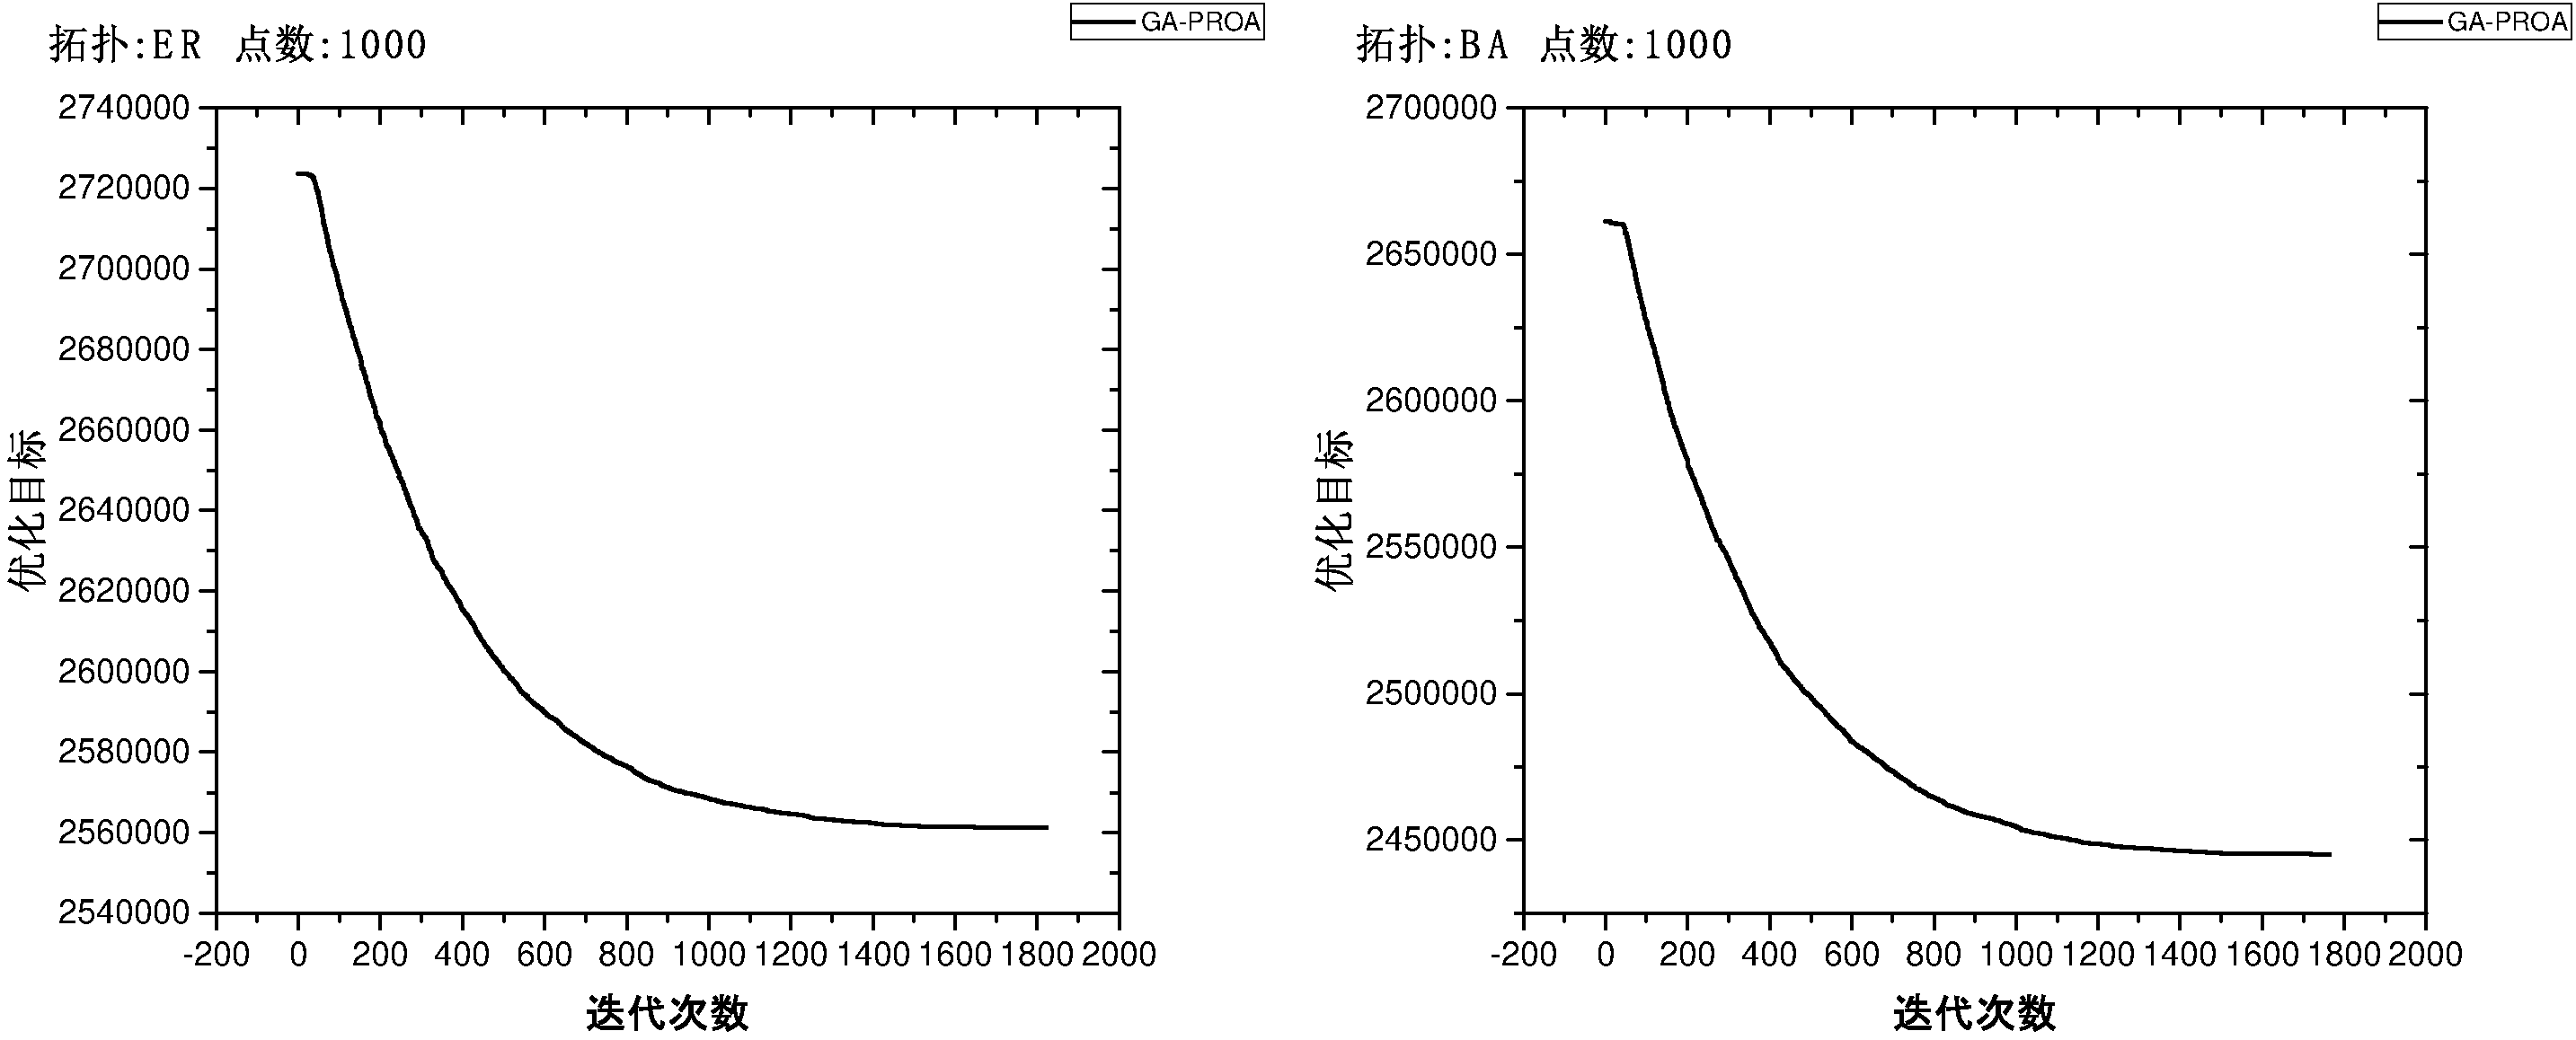
\includegraphics[width=1 \textwidth]{figures/CO-GA-1000.pdf}}
    \end{center}
  \caption{{\footnotesize{objective-task}}}
  \label{IterNum}
\end{figure}
\begin{figure}
\setlength{\belowcaptionskip}{-0.1cm}
  \begin{center}
    {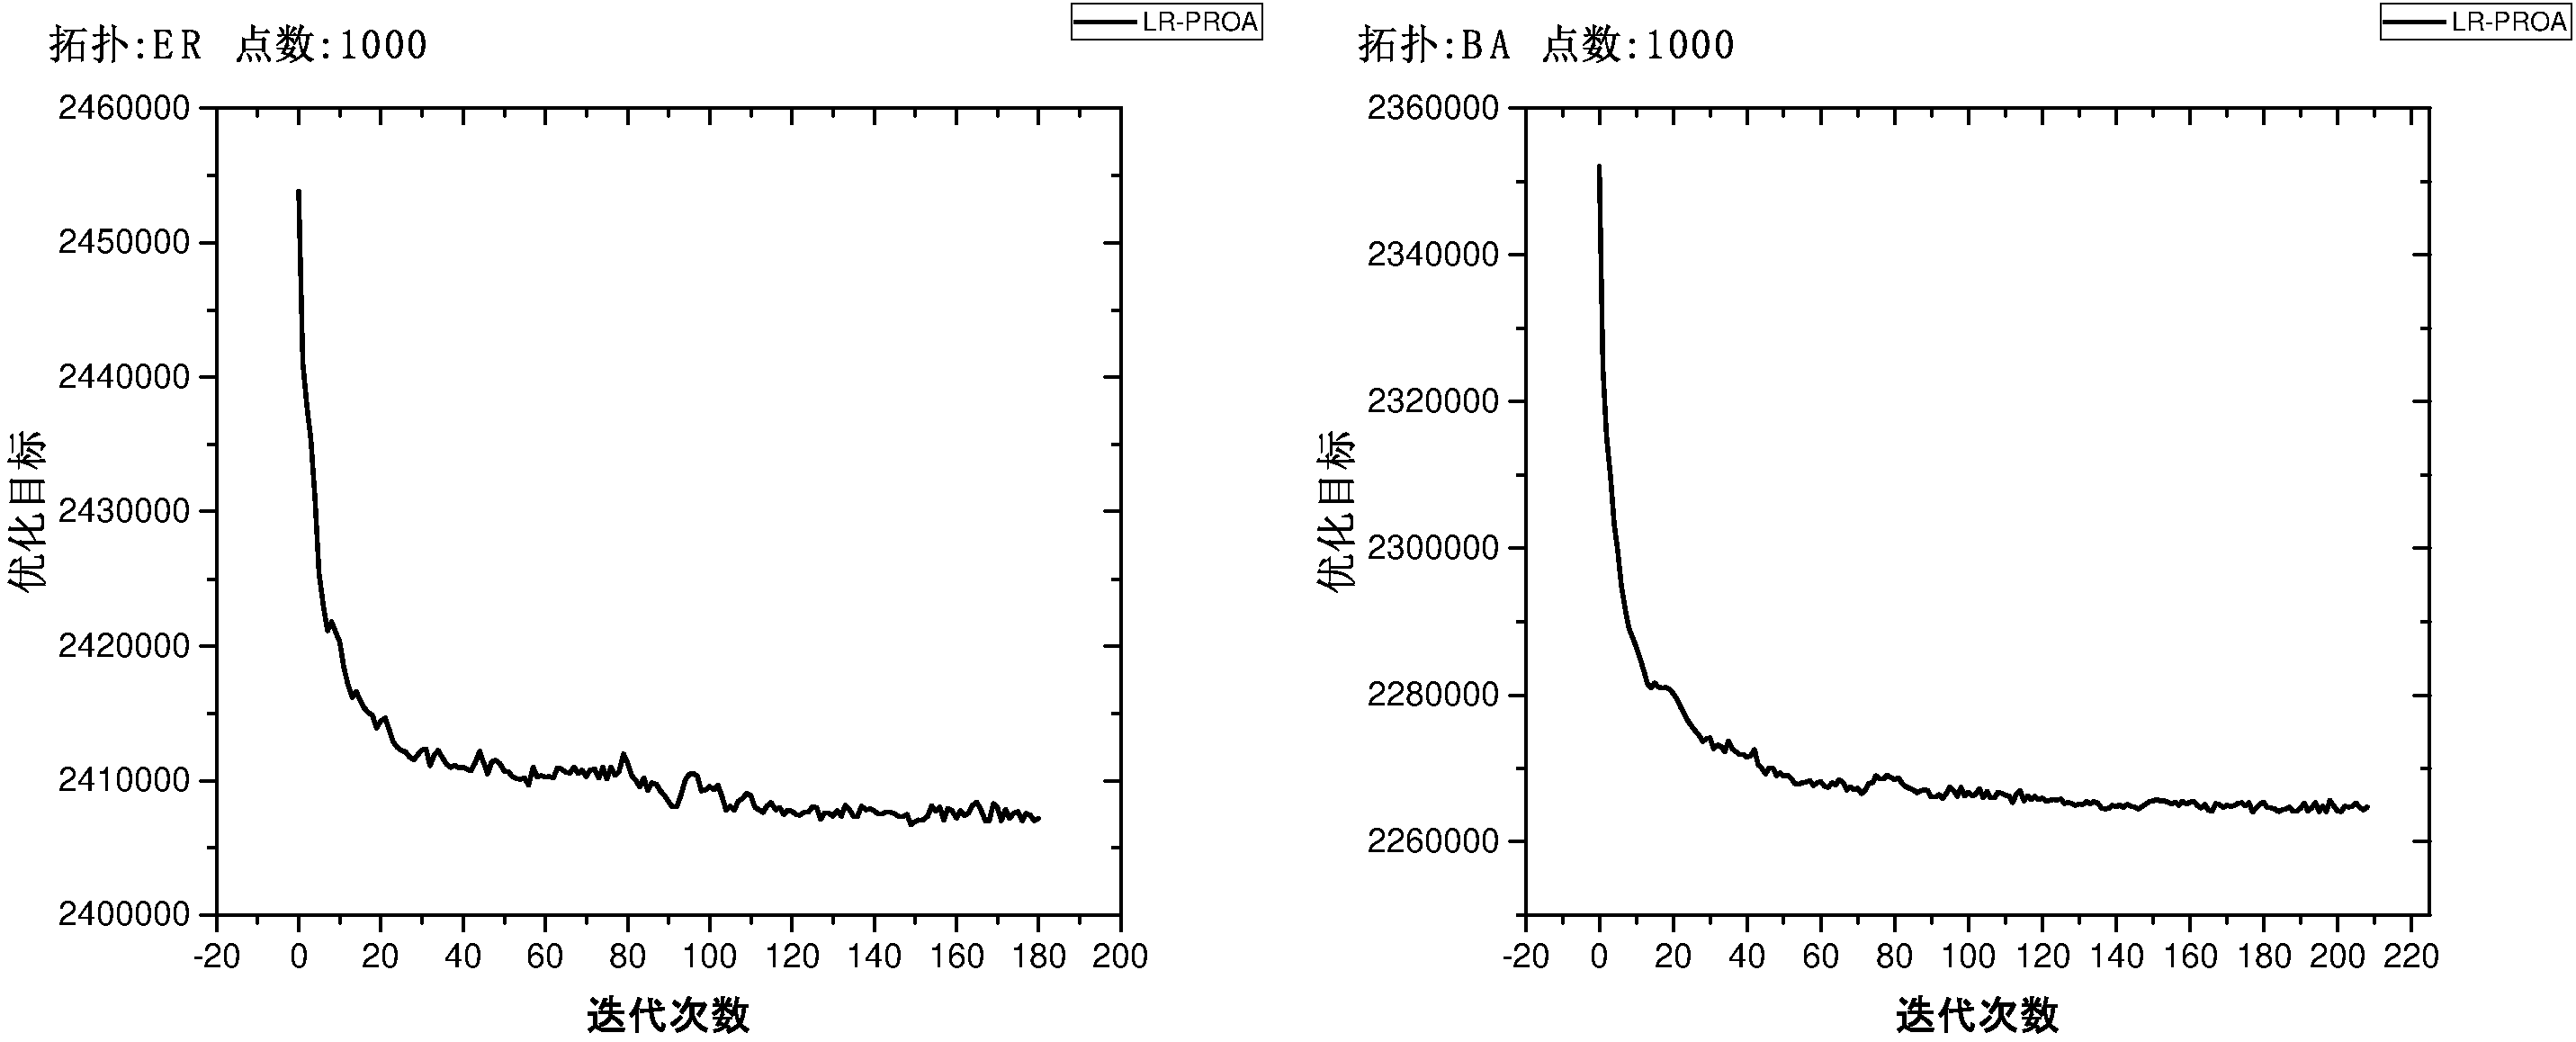
\includegraphics[width=1 \textwidth]{figures/CO-LR-1000.pdf}}
    \end{center}
  \caption{{\footnotesize{objective-task}}}
  \label{IterNum}
\end{figure}







% !Mode:: "TeX:UTF-8"

\chapter{分层光网络下的并行路由优化算法研究}
\section{引言}
随着视频流、云计算服务和移动应用的普及,互联网的流量不断增加 \citing{EINC},业务量的持续增长给互联网的传输带来了巨大的挑战,为了满足日益增长的容量要求,波分复用(WDM)系统已部署在骨干网络,其每个通道带宽高达40 GB/s或100 Gb/s。 现在,400 Gb/s 的带宽接口已经在实验室 \citing{ELAB} 实现,此外,为了满足不同的数据速率服务异构的流量类型,混合线路速率(10/40/100Gb/s)的WDM 系统也已经部署 \citing{EDF}。因此,WDM 光网络视乎为大流量业务传输提供了一个既实际又高效的解决方案。
然而,传统的WDM光网络严格遵循ITU-T的固定均匀间距和网格(通常为50)GHz或100千兆赫) \citing{ETR},这样会导致低效的频谱利用率,比如,一个较大的波长可能会被分配给一个低速率的业务,即使这个业务根本就不能占满整个波长。很明显,传统WDM 光网络的不灵活和粗粒度的带宽控制会导致显著的频谱浪费,限制了提高其网络容量的潜力。

为了应对WDM网络的低敏捷性和频谱浪费问题,近年来,弹性光网络(EON)的架构被提出,在EON架构中,存在细粒度的带宽间隙(比如,12.5GHZ),他比WDM 网络所遵循的ITU 标志的50GHZ或者100GHZ 的带宽粒度要小很多,而且,这些带宽间隙可以根据需要被组合在一起以提供更宽的通道。所以为了提高带宽利用率,在EON 中存在混合速率,每个速率的业务需要不同数量的频谱间隙数量。理论上,EON能够灵活地提供各种速率,但是在实际中,EONs却可能只含有很少的速率种类,这主要是因为:第一,随着频谱的增加,频谱碎片和管理复杂度将显著增加。第二,实际的EON从较低的线路费率升级到更高的线路费率,并存大量速率的情况已经很少见了。

为了在EON网络中加入业务,控制平面必须在网络中找到一条路径,同时,还需要在此路径上的链路上分配足够的频谱带宽,来创建一个合适的端到端光路连接,这被称为路由和频谱分配(RSA)问题,EON中的RSA 问题比传统的在WDM网络中的路由和波长分配(RWA)问题更具有挑战性,传统的RWA解决方案\citing{ETRP1,ETRP2} EONs中已经变得不再适应了。在EONs中一个业务需求可能需要多个连续的频谱间隙,而且由于缺少全光谱转换器,每条光连接的频谱从它的源节点到它的目的节点 ,在所经过的链路上保持不变,这被称为频谱连续性限制。

RSA问题可以进一步分为静态RSA问题和动态RSA问题。静态的RSA问题出现在网络规划阶段,其中流量需求是已知的,这样可以离线计算出最优或者接近最优的RSA 解,动态RSA 问题是指在实时业务情况下光通路的路由选择和波长分配的优化问题,在动态RSA 问题中,业务随机的到达和离开光网络,而且当业务到达网络时,控制平面需要在短时间内找到RSA解来安排业务。动态RSA 问题比静态RSA问题更具有挑战性,因为业务需求随机到达和离开,网络状况随时发生变化,而且要求控制平面反应实时。

链路代价表示路由路径选择这一条链路所需要的代价,链路代价可以设置为链路延迟,租用链路需要的费用等等,业务的路由代价表示业务路径经过的链路的代价总和,路由代价反应了路由路径的优劣程度,如果链路代价设置为延迟,则路由代价越小表示路由整体延迟较小,如果链路代价设置为1,则路由代价越小,表示路径经过的跳数越小,使用的链路资源越小。
本章考虑在EONs中解决动态RSA问题,设计出带跳限约束下的基于分层图的动态路由优化算法来优化整体路由代价,分别考虑无权图和带权图上的算法GPU加速设计,GPU 并行版本达到平均近5倍的算法加速比,实验与分层图上的传统算法比较,显示该算法过程在短时间内能够大量的优化路由代价,并且由于路由选择较优,使用网络资源较少,最终网络阻塞率表现也有显著的提高,实现了快速的路由代价优化和整体的阻塞避免。
\section{问题描述}
\subsection{EON中动态RSA问题}
在动态场景中,业务的到达时间和服务时间都是随机的,当业务到达网络时,SDN 控制层需要找到可行的路径,并且为路径分配合适的频谱资源。由于EON 的物理限制,RSA问题的解需要满足以下限制:

第一,传输距离限制:光信号的传输质量会随着传输距离的增加而下降,为了在目的点顺利恢复光信号,光链路的传输距离需要小于一个阈值$W_{max}$, 为了简化设计,本文假设每一条链路的长度相同,都是一个单位,那么传输路径的跳数需要小于阈值$D_{max}$。

第二,频谱连续性限制:每条光连接的频谱从它的源节点到它的目的节点 ,在所经过的链路上保持不变。

第三,频谱不重叠限制:同一光纤链路中的频谱不能分配给不同的光路。

第四,频谱邻近限制:频谱邻近约束保证分配给一个光路径的频谱必须是一个连续的部分。
\subsection{分层网络模型}
论文 \citing{ELAYER}中提出一种分层图模型来解决WDM网络中的路由和波长分配问题,分层图模型将路由选择和波长分配问题统一到一起来,使得RWA 问题变得简化,这种分层图模型也可以很容易推广到EONs 的RSA 问题中。

我们使用有向图$N(V,E)$表示物理网络拓扑,其中$V={v_1,v_2,...,v_N}$表示节点集合,$E={e_1,e_2,e_3,...,e_M}$表示边集合,$e_k=(i_k,j_k)$表示边的头节点为$v_{i_k}$,边的尾节点为$v_{j_k}$。假设所有光链路具有相同的频谱范围$W=(F_{start},F_{end})$, 其中$F_{end}-F_{start}=C$。EON 所支持的速率集合为$R$, 比如,$R={40Gb/s,100Gb/s,400Gb/s}$, 每一种速率$r\in R$ 需要一个特定的频谱宽度$b_r GHz$。一个源节点为$s$,目的节点为$t$, 速率为$r Gb/s$的业务被表示为$TD(s,t,r)$。
下面我们讨论分层图的产生过程,假设第一个速率的为$r$的业务$TD_r(s,t)$到达网络,我们从可用的频谱切割出一块频谱大小为$b_r$ 的连续带宽分配给速率为$r$ 的业务,假设这块频谱的起始频率为$fs_{( r,1 )}$,终止频谱为$fe_{( r,1 )}$,那么$fe_{( (r,1) )}-fs_{( (r,1) )}=b_r$,我们把所有物理链路上频谱范围$( fs_{( (r,1) )},fe_{( (r,1) )} )$,从所有链路上切割下来,把切割下来的部分组成一个新的虚拟网络$N^{( r,1) )} ( V^{( (r,1) )},E^{( (r,1) )}) )$,在这个新的网络中每条链路的频谱范围都是$(fs_{( (r,1) )},fe_{( (r,1) )})$,这样切割下来之后,原来的物理网络的频谱范围更新为$( F_{start}+b_r,F_{end} )$。
如果在这个复制出来的图上为业务求一条最短路径$p$,那么容易知道路径$p$一定满足约束2,3,4, 这样问题被简化为单纯的路由问题。要注意的是,这个虚拟图上频谱不能再分配给其他速率为$r'$ 的业务$TD_{r'}(s',t')$, 即使$b_r'<b_r$,这是因为这样会产生大量的频谱碎片,使得频谱利用率下降,阻塞率降低,并且这样会使得问题变得更加复杂化,所以这些分割出来给速率$r$的频谱,将继续被分配给速率为$r$ 的业务。当下一个速率为$r$的业务$TD_r (s'',t'')$ 到达网络后,他首先在图$N^{( r,1) )} ( V^{( (r,1) )},E^{( (r,1) )}) )$中寻找路径,如果找到合适的路径则加入网络并且更新路径链路的可用频谱为0;反之,如果他在图$N^{( r,1) )} ( V^{( (r,1) )},E^{( (r,1) )}) )$中没有找到合适的路径,那么算法会重新去”切割“物理拓扑得到虚拟网络$N^{( r,2) )} ( V^{( (r,2) )},E^{( (r,2) )}) )$,这样随着大量业务的动态的到达和离去,会产生大量的分层图,频谱资源已经大量地分布在各个虚拟图中,我们把这些虚拟图叫做分层图(layered Graph),现在RSA问题转化为在分层图中求解路由的问题,问题被简化。
下图 \ref{layer}表示分层图示意,原图被切割成一个分层图集集合$L$,$L_i \in L$表示速率$i$的分层图集,如图所示,速率$k$的一共有$|L_k|$ 个图副本,每个子分层图占用频谱$(fs_{( (r,1) )},fe_{( (r,1) )})$,图 \ref{layer}中,点$v_i^{( (r,l) )}$表示速率$r$ 的第$l$ 层图上的第$i$ 号点。
\begin{figure*}
\setlength{\belowcaptionskip}{-0.5cm}
\begin{center}
{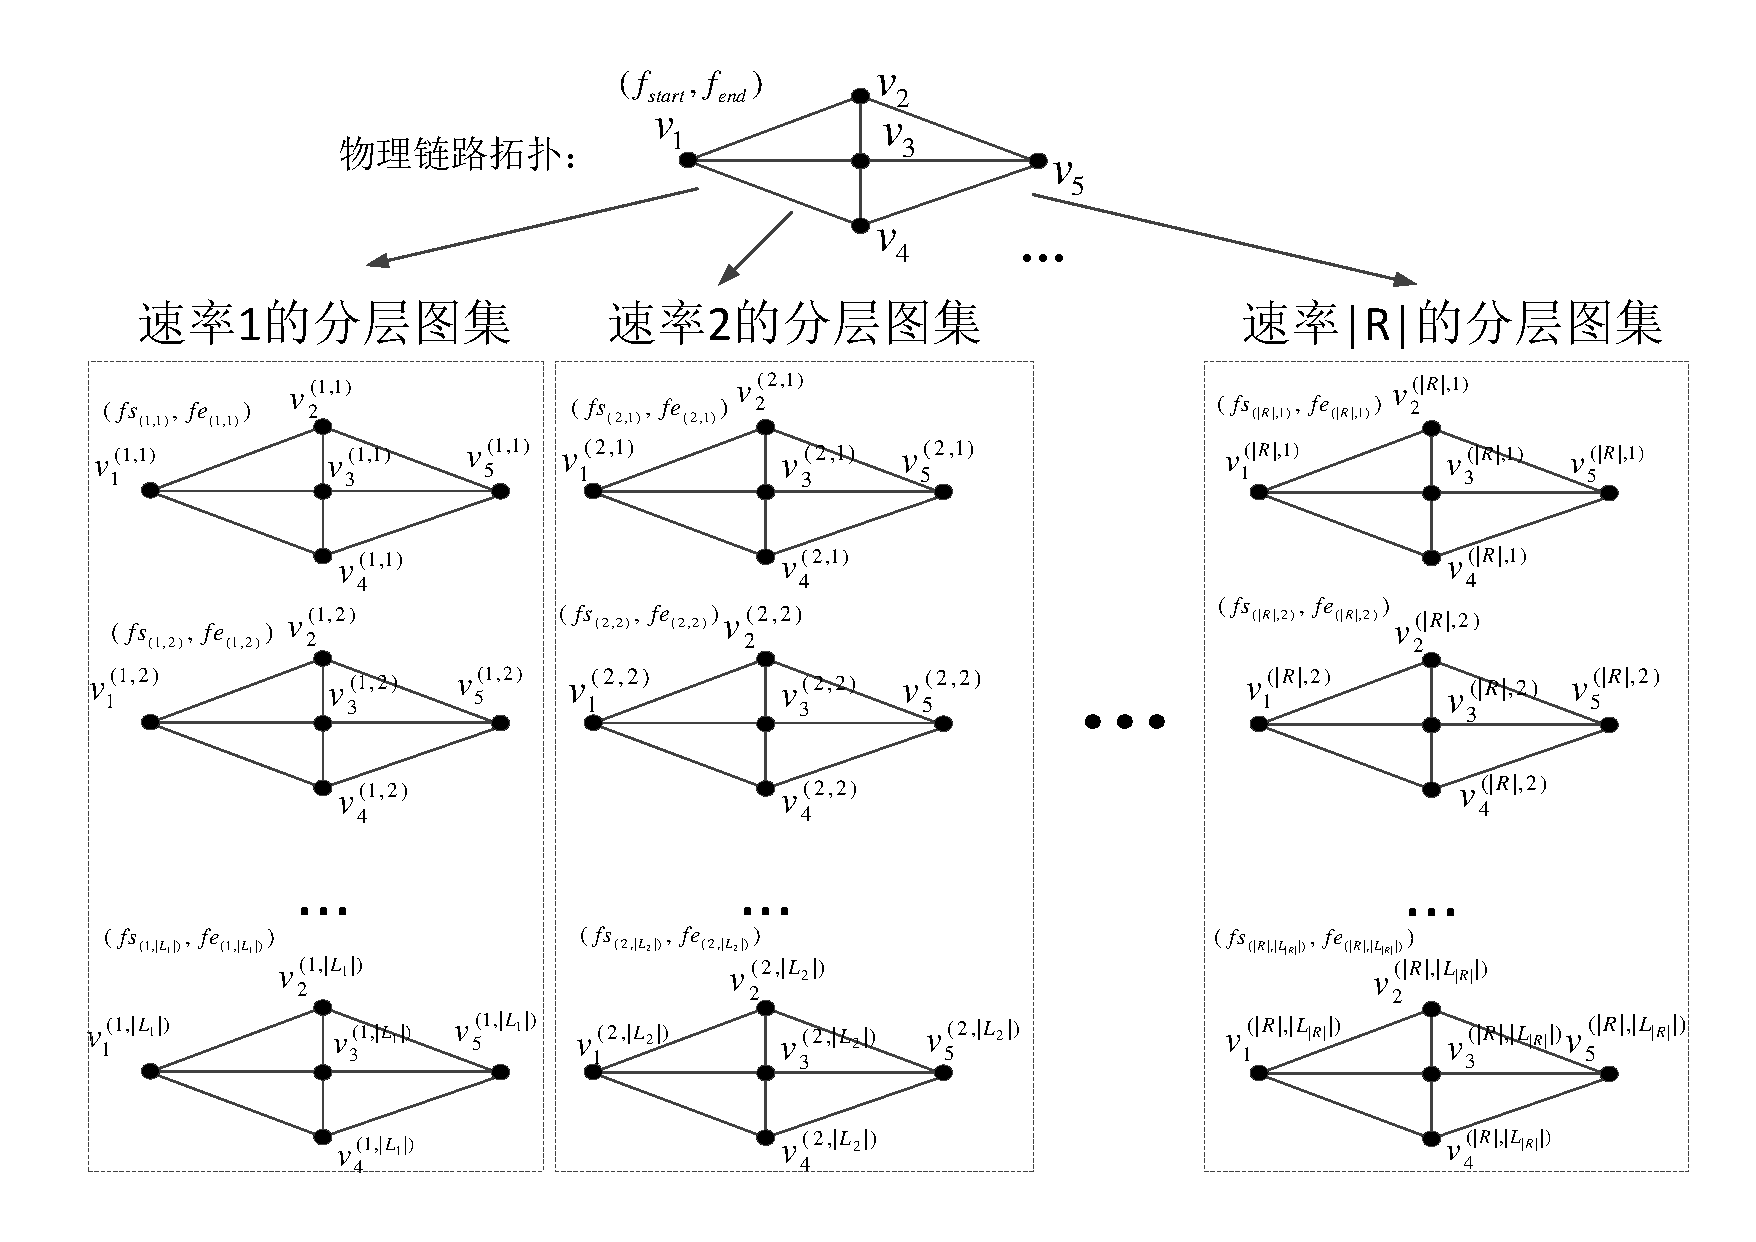
\includegraphics[width=1 \textwidth]{figures/LAYER.pdf}}
\end{center}
\caption{{\footnotesize{分层图示意}}}
\label{layer}
\end{figure*}
\section{主要优化流程}
根据前面的讨论,当一个速率为$r$的业务$TD_r(s,t)$到达网络时,一共有$L_r$ 个分层平面都可以用于此业务,也就是说如果在这些图当中都能为业务找到合适的路径的话,那么业务就有$L_r$ 条路径可供选择,我们可以选择代价最小的一条来优化路由。进一步,当有一批速率为$r$ 的业务集合$TD_r$到达网络时,如果大家都选择同一层加入的话,会出现大量的冲突,而且路由代价也会很大,但是由于现在有多个分层图平面可以选择,每个业务都有$L_r$条路径可以选择,这就给路由优化提供了可能,不同的业务需求可以选择不同层上的路径来进行路由,以使得总体路由代价减小,节省网络频谱资源,从而优化阻塞率。

本节提出一个基于分层图的动态RSA路由优化算法流程称为带路由优化的RSA算法(route optimization RSA,RORSA),算法流程如下图 \ref{bblayer}所示:
\begin{figure*}
\setlength{\belowcaptionskip}{-0.5cm}
\begin{center}
{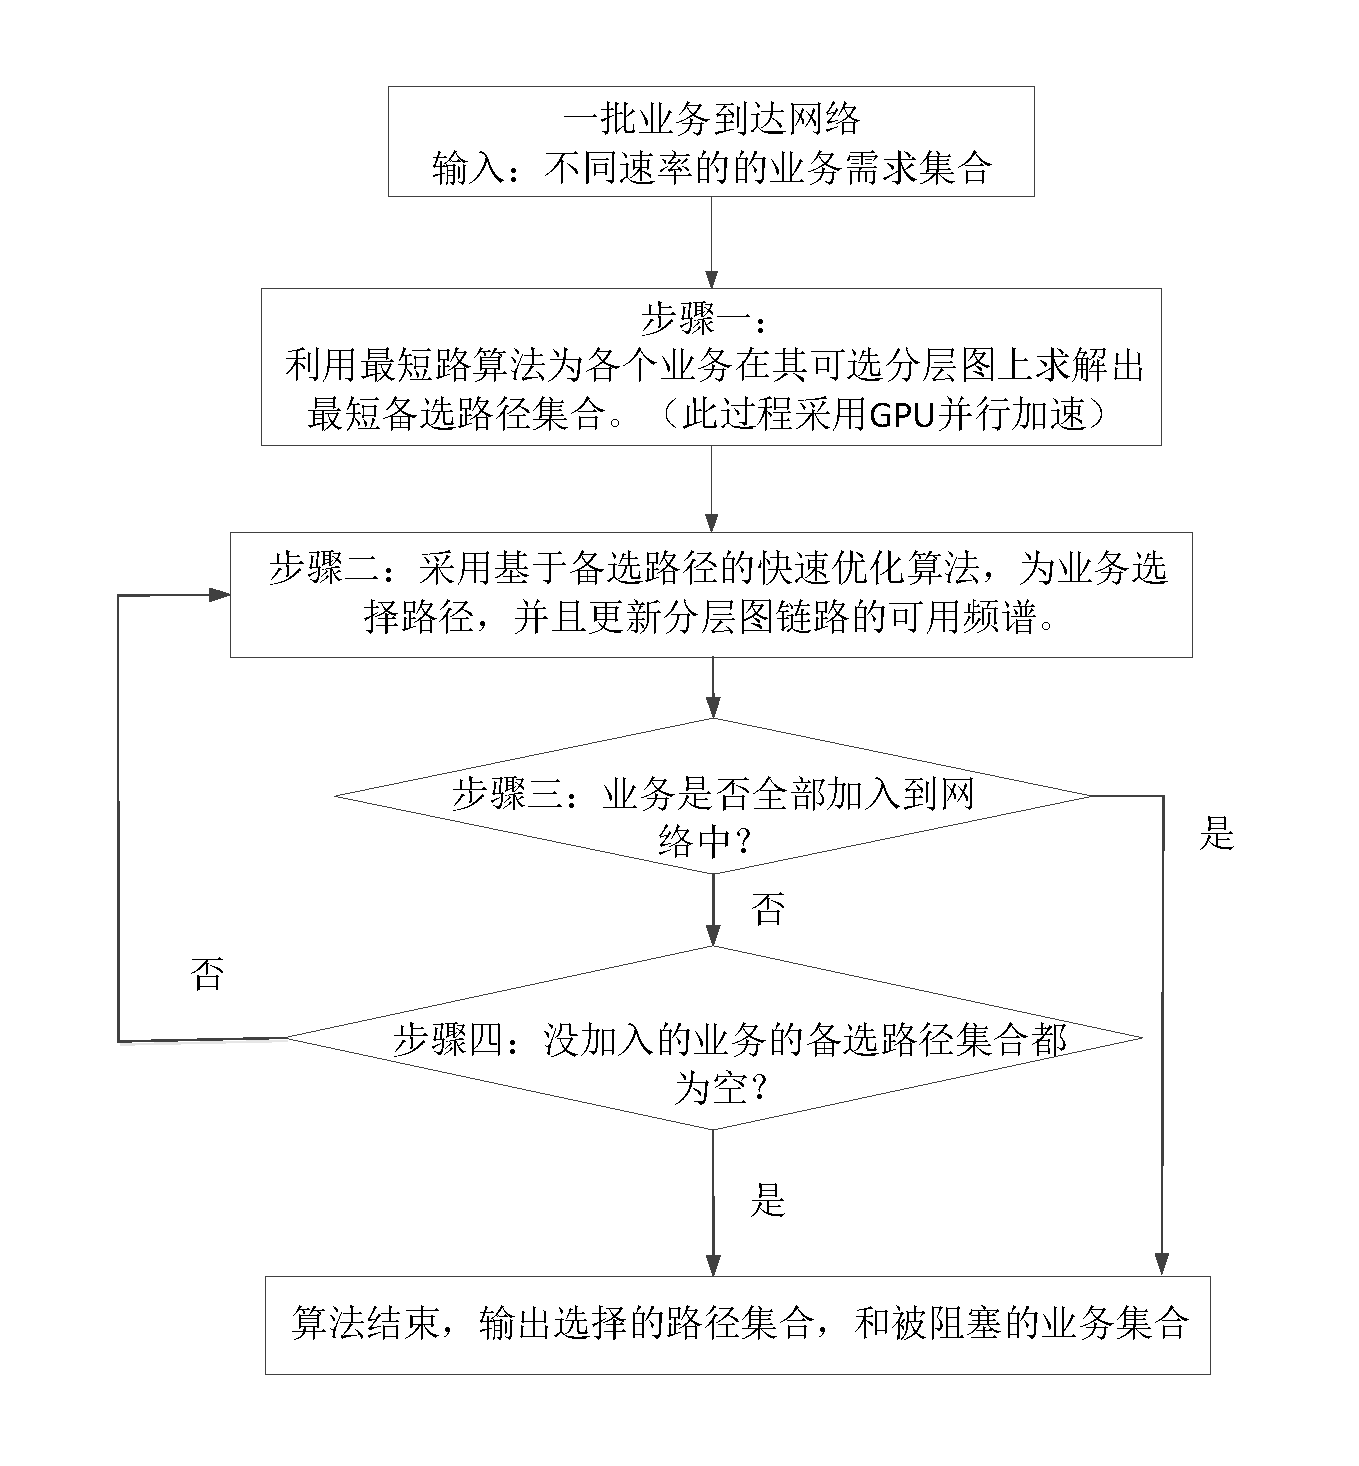
\includegraphics[width=1 \textwidth]{figures/bbprocess.pdf}}
\end{center}
\caption{{\footnotesize{算法优化流程}}}
\label{bblayer}
\end{figure*}
当一批业务到达网络时,对每一个业务在其对应速率的层上求出大量的备选路径,这个过程计算量较大,但是每一个拓扑层是独立的,所以可以采用并行算法来进行加速设计,后面4.4和4.5将讨论无权图和有权图上的两种基于GPU 的路由加速算法来加速这个步骤,当备选路径都求出来了之后采用一种快速路径选择算法来把业务安排进网络,这个步骤采用一种简单贪心的启发式算法,由于备选路径较多,实验发现这种简单的贪心算法已经可以很好的优化路径代价了。当业务的路径确定后,如果每个业务都能加入到网络,那么本轮算法结束,如果还有剩余的业务没有被安排进网络,需要判断业务的备选路径集合是否为空,如果为空,则说明所有层都不能为业务求出路径,业务将被阻塞;反之,如果业务的备选路径集合不是空,则说明业务是因为和其他业务的路径冲突而导致不能被安排进网络,分层图中可能还存在其他可用路径,所以需要重新在分层图中计算路径,算法回到步骤二,对这些业务进行重新计算。

步骤一的具体算法将在4.4和4.5介绍,这里介绍步骤二的快速优化算法,快速优化算法的主要思想是根据求出来的备选路径为每个业务选择路径以使得整体路径代价最小,由于动态RSA环境下需要在短时间内安排好路径,所以为了提高计算速度,这里采用一种简单快速的贪心算法来进行解决,流程如算法\ref{arrange}所示。
\begin{algorithm}[htb]
\begin{algorithmic}[1]
\Require
$N(v,E)$:分层图;
$P$:备选路径集合;
$TD$:业务需求集合;
\Ensure
$AP$:加入业务的路径集合;
\For{$T \in TD$}
\State {对$P_T$中的路径按照路径的代价进行降序排序}
\EndFor
\State {对$T$按照$P_T$中的最小路径代价进行排序}
\For{$T \in TD$}
\For{$p \in P_T$}
\If{路径$p$所对应分层图上的相应链路没有被占用}
\State{把$p$加入到$AP$中,并更新$p$所对应的分层网络上的链路,跳出for循环,以继续为下一个业务选路}
\EndIf
\EndFor
\EndFor
\end{algorithmic}
\caption{路径选择算法}
\label{arrange}
\end{algorithm}

算法开始对每个业务的备选路径按照其代价进行降序排序,也就是每个业务优先会选择代价较低的备选路径。然后,再对业务按照其最小代价的路径进行排序,这样保证优先考虑代价小的业务。然后开始加入业务到网络,对每一个业务,遍历其已经排序好的备选路径,如果在相应分层图上路径包含的链路都是空闲的,则加入业务到网络中,更新分层图上的相应链路为占用状态,把这个路径$p$ 加入到集合$AP$ 中。最后算法输出路径集合$AP$, 算法结束。
\section{无权图情况下的GPU算法设计}

无权图情况下,路由的代价就是路径的跳数,跳数越少说明占用的网络资源越少,尽量优化路径的跳数可以节省网络资源,进一步的降低动态情况下的网络的阻塞。无权图情况下的路由算法一般使用BFS (宽度优先搜索)算法进行求解,BFS 算法从目的节点最近的点开始,一层一层的进行扩展直到找到目的节点,每扩展一层跳数增加一条,扩展一层需要遍历大量的边,这些边的扩展操作是相互独立的,所以为算法提供了并行设计的可能性,在加上不同速率不同层上的路由求解上的并行,总体并行粒度是很大的,下面分别对不同的并行层次的设计进行讨论。
\subsection {相同速率业务的并行}

如下图 \ref{bfs}所示,对速率都为$r$的一批业务,在其可用的每个分层图上并行进行计算,在每个分层图上,具有相同源节点的业务组成业务组,因为他们的路径可以一起计算,对每一个业务组,在GPU 上开辟$|E|$个线程对每一条边进行扩展操作,那么整个过程的的并行粒度为$|L_r||D_r||E|$, 其中$|D_r|$为速率为$r$ 的业务组数量。
\begin{figure*}
\setlength{\belowcaptionskip}{-0.5cm}
\begin{center}
{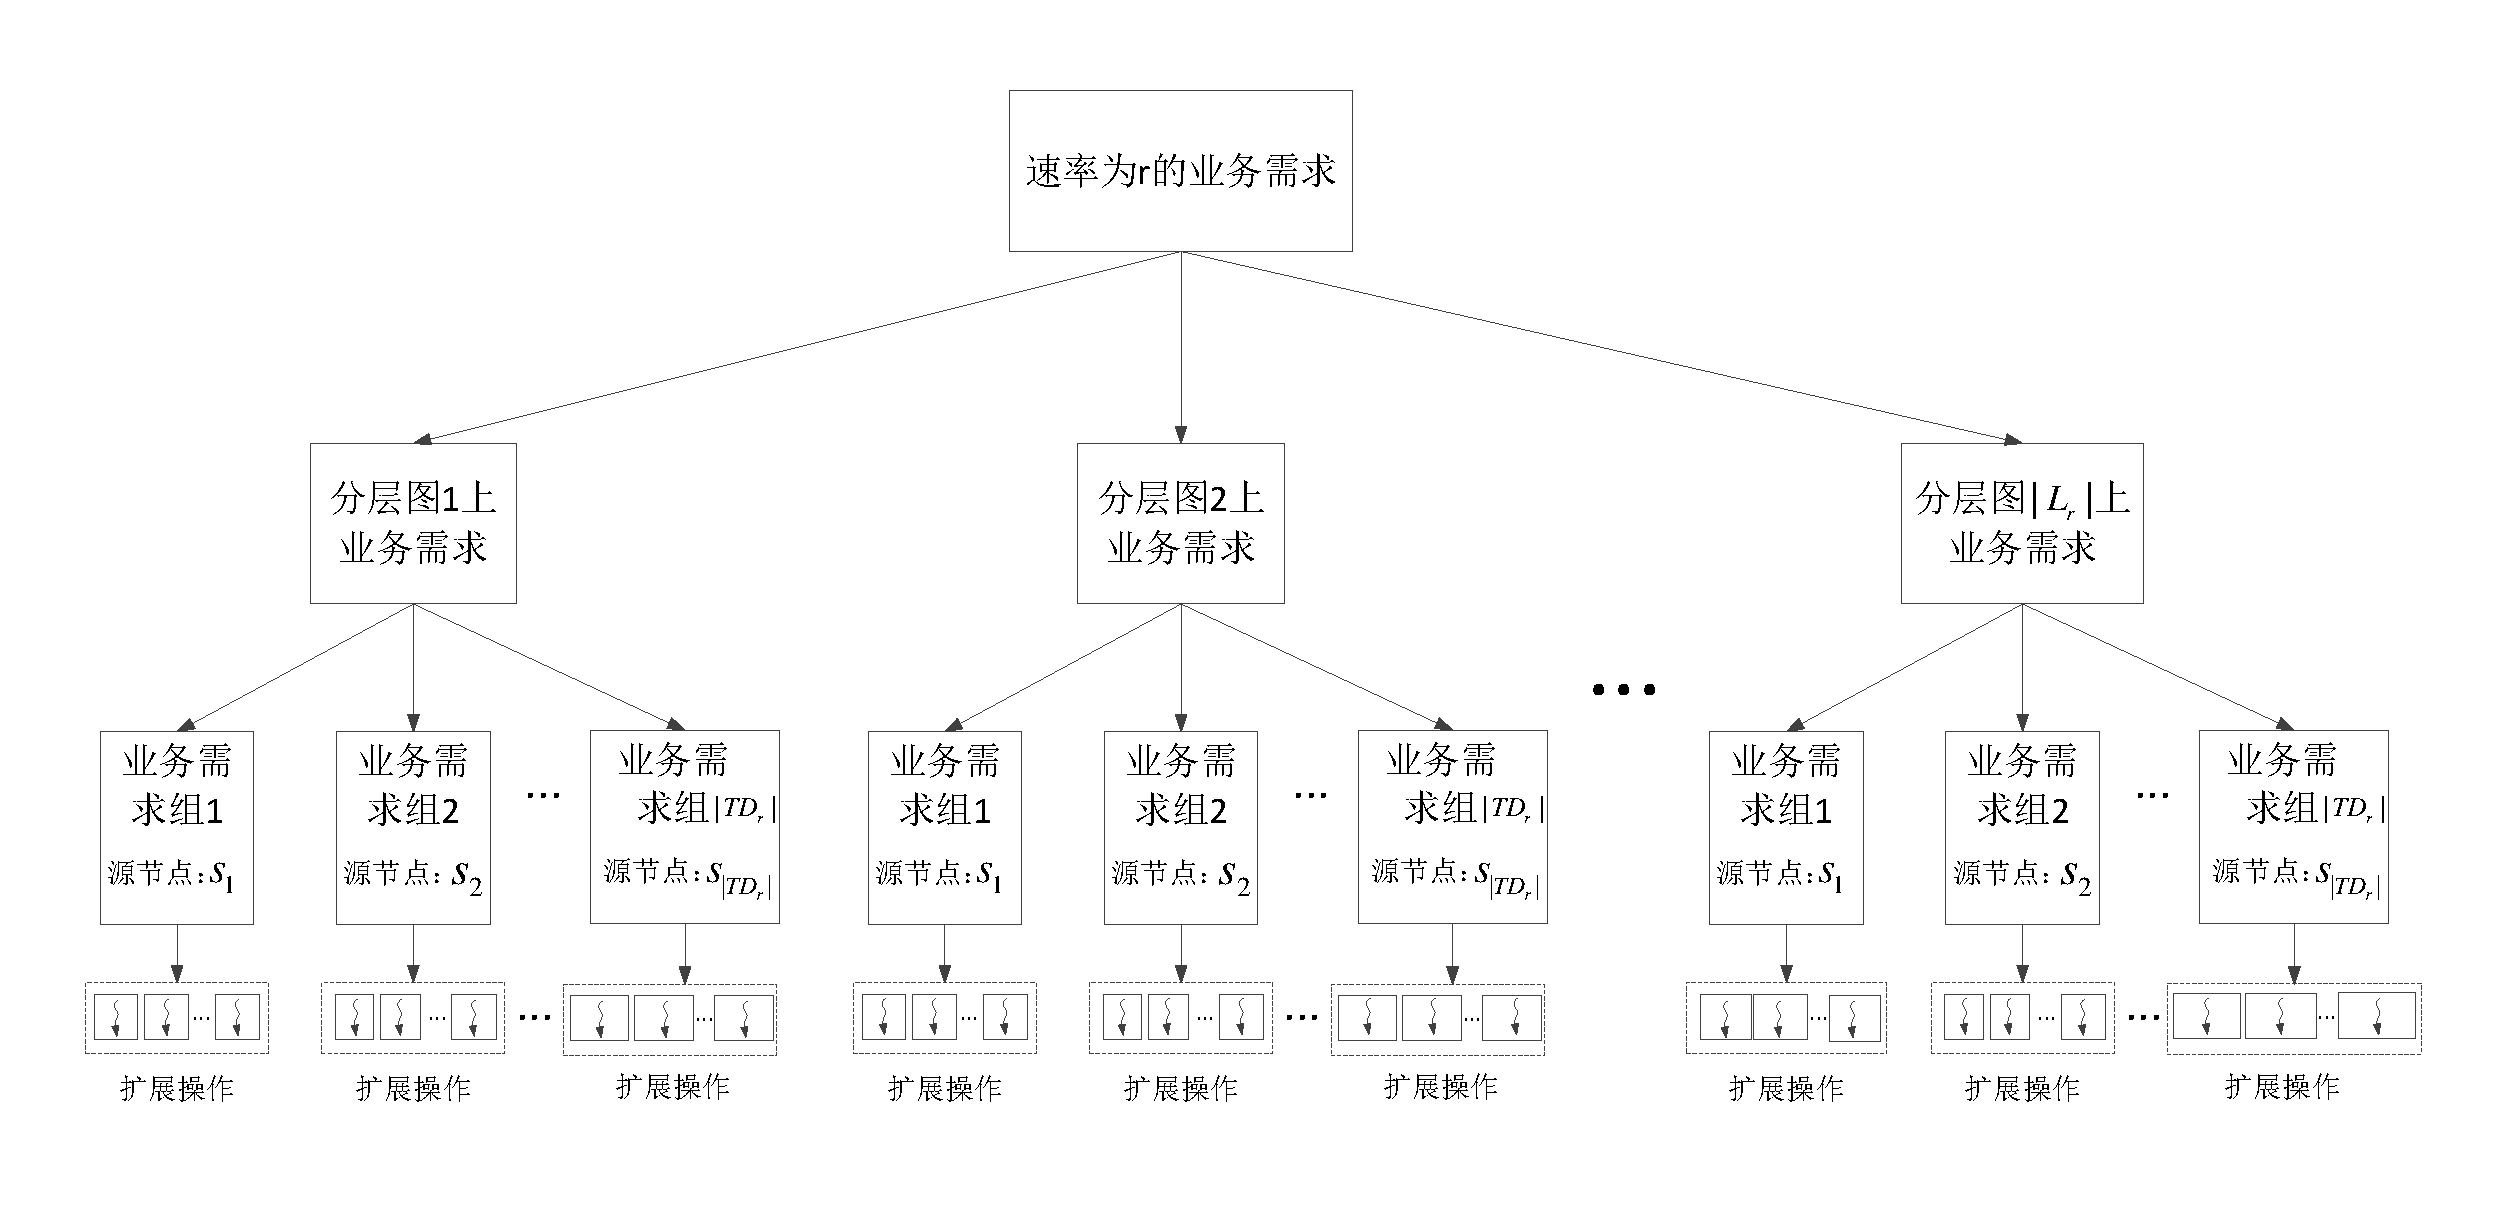
\includegraphics[width=1 \textwidth]{figures/bfs.pdf}}
\end{center}
\caption{{\footnotesize{bfs并行示意图}}}
\label{bfs}
\end{figure*}
\subsection{不同速率间业务的并行}
由于动态业务情况下每次到达网络的业务数和速率情况都是变化的,不同速率之间业务的并行不容易直接实现在一个kernel 中进行,我们采用GPU提供的流并行进行并行设计。如下图 \ref{bfssteam}所示:
\begin{figure*}
\setlength{\belowcaptionskip}{-0.5cm}
\begin{center}
{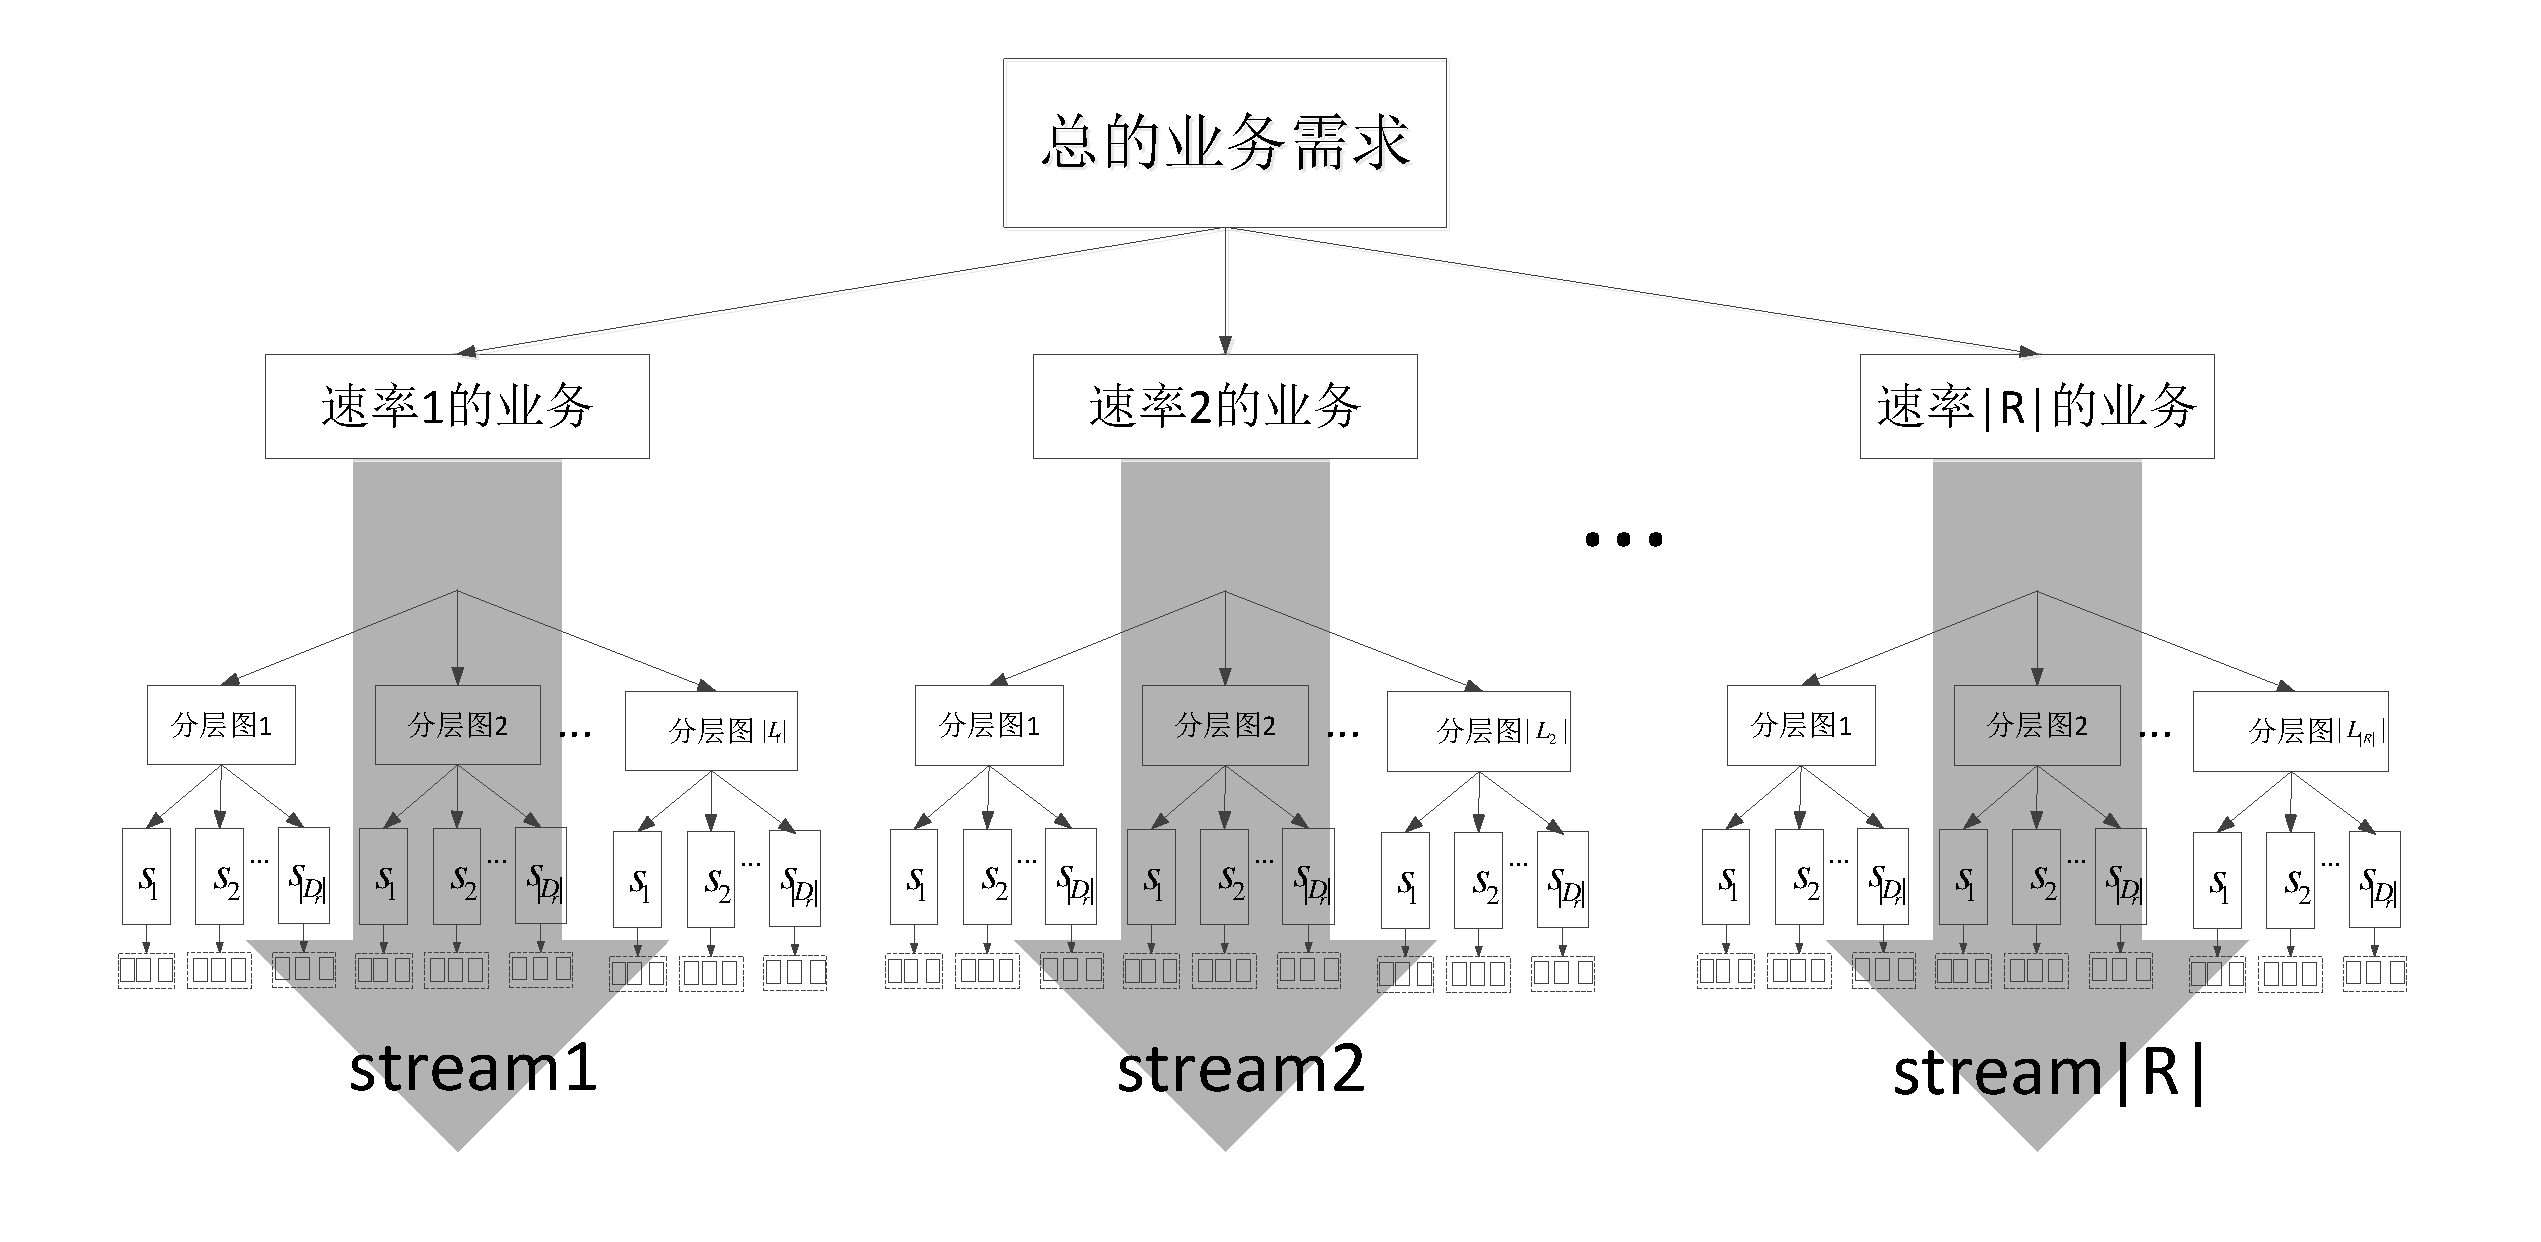
\includegraphics[width=1 \textwidth]{figures/hbfs.pdf}}
\end{center}
\caption{{\footnotesize{bfs流并行示意图}}}
\label{bfssteam}
\end{figure*}
我们为每一个速率建立一个stream来负责这个速率的业务计算,假设业务一个有$|R|$个不同速率,那么需要建立$|R|$个stream,多个kernel 同时执行,充分利用GPU 的SMIT资源,当SIMT资源足够时,每个kernel将并行执行,当SIMIT不足时,不同的kernel之间可以进行快速的切换,以达到隐藏延迟的效果。

\subsection{GPU上kernel设计}
和3.4.2中讨论不一样,在BFS的并行中不会存在前驱节点更新的同步问题,但是,我们依然需要两个kernel函数,这是因为扩展kernel 需要执行多次,如果扩展和更新同时执行,那么更新也会执行多次,这会增多内存访问,所以我们把两个操作分成两个kernel,一个$kernel\_bfs\_extend$ 进行边的扩展操作,一个$kernel\_bfs\_update$ 进行前驱节点的更新操作,其中$kernel\_bfs\_extend$需要多次调用,但是$kernel\_bfs\_update$ 只需要在最后执行一次。
\begin{algorithm}[t]
\begin{algorithmic}[1]
\Function{kernel\_bfs\_extend}{$E$, $Dist$,$rid$,$round$}
\State {$bid \leftarrow$ block ID}
\State {$tid \leftarrow$ thread ID}
\State {用$(bid,tid,rid)$ 映射到边的标号$eid$}
\State {用$(bid,tid,rid)$ 映射到分层图标号$lid$}
\State {$e \leftarrow E[gid][eid]$}
\If {$e.avaliable==-1$}
\State{return}
\EndIf
\State {用$(bid,tid,rid)$ 映射到的源点标号$sid$}
\If{$Dist[lid][sid][e.head]>round $\&\&$ Dist[lid][sid][e.tail]+1==round$}
\State {$Dist[gid][sid][e.head] \leftarrow round$}
\EndIf
\EndFunction
\end{algorithmic}
\caption{kernel\_bfs\_extend}
\label{KernelBFS}
\end{algorithm}
在$kernel\_bfs\_extend$中,输入$E$是所有的分层图的边所组成的集合,$Dist$是预先分配的距离标记数组,他是一个三维数组,第一维表示当前距离数组对应的分层图标号,第二维度表示源节点,第三维度表示目的节点,比如$Dist[3][10][5]$=4表示在第3 个分层图上,点10到3 的距离为4,初始时,除了源节点距离被初始化为0之外,其他的距离都被初始化为无穷大。$rid$ 表示当前kernel 负责的计算的业务速率标号,他是区分不同流的标记,$rid$ 不同表示执行kernel 的流不同。$round$ 表示当前扩展的层数,由于BFS是一层一层进行扩展操作,我们需要记录当前层数来决定哪些边需要扩展。算法开始时先进行一系列映射操作,将线程映射到边标号$eid$, 当前所在分层图标号$lid$,以及源节点标号$sid$。 由于动态情况下,边的可用状态可能发生变化,找到边之后,需要判断这条边是否可用,如果不可用则返回。接着判断当前边是否可以进行扩展操作,如果尾节点已经更新过了($Dist[lid][sid][e.head]<=round$),则不能再更新了,反之,还需要判断头节点是否上一次扩展层的节点($Dist[lid][sid][e.tail]+1==round$),如果是的话,那么就更新尾节点的距离为当前扩展层$round$。
\begin{algorithm}[t]
\begin{algorithmic}[1]
\Function{kernel\_bfs\_update}{$E$, $Pre$,$rid$}
\State {$bid \leftarrow$ block ID}
\State {$tid \leftarrow$ thread ID}
\State {用$(bid,tid,rid)$ 映射到边的标号$eid$}
\State {用$(bid,tid,rid)$ 映射到分层图标号$lid$}
\State {$e \leftarrow E[gid][eid]$}
\If {$e.avaliable==-1$}
\State{return}
\EndIf
\State {用$(bid,tid,rid)$ 映射到的源点标号$sid$}
\If{$Dist[lid][sid][e.head]==Dist[lid][sid][e.tail]+1$}
\State {$Pre[gid][sid][e.head] \leftarrow e.tail$}
\EndIf
\EndFunction
\end{algorithmic}
\caption{kernel\_bfs\_update}
\label{KernelBFS}
\end{algorithm}
在$kernel\_bfs\_update$中,其主要逻辑和$kerne\l_bfs\_extend$一样,在进行更新判断的时候,判断当前边的头节点是否是尾节点的上一层(Dist[lid][sid][e.head]==Dist[lid][sid][e.tail]+1)如果是的话,那么头节点就有资格作为尾节点的前驱节点,于是进行前驱更新操作。
介绍完了两个kernel之后,算法 \ref{ParaSPC}为整个并行BFS的算法流程:
\begin{algorithm}[t]
\begin{algorithmic}[1]
\Require
业务需求集合$TD$;
分层图链路集合$E$;
\Ensure {业务需求的最短路径集合$P$}
\State {将业务根据速率和源节点重新组合成业务分组集合$D$}
\For {$D_r \in D$}
\For {$d_{rs} \in D_r$}
\For {$l \in L_r$}
\For {$v \in V$}
\If {$v==s$}
\State {$Dist[l][s][v]\leftarrow$ 0}
\Else
\State {$Dist[l][s][v]\leftarrow \infty $}
\EndIf
\State {$Pre[l][s][v]\leftarrow -1 $}
\EndFor
\EndFor
\EndFor
\EndFor
\State {新建$|R|$个流,组成集合$S$}
\State {$round \leftarrow$ 1}
\While{$round<=W_{max}$}
\For{r in R}
\State {在流$S_r$上发射 kernel\_bfs\_extend($E$, $Dist$,$r$,$round$)}
\EndFor
\State{round=round+1}
\EndWhile
\For{r in R}
\State {在流$S_r$上发射 kernel\_bfs\_update($E$, $Dist$,$r$,$round$)}
\EndFor
\State {根据前驱数组$Pre$重建路径,然后把路径加入到集合$P$}
\end{algorithmic}
\caption{{并行bfs计算}}
\label{ParaSPC}
\end{algorithm}
算法 \ref{ParaSPC}开始时先将业务按照速率的不同进行划分,再将业务按照源节点的不同划分成不同的业务组集合$D$,比如,$D_r \in D$ 表示速率为$r$ 的业务组集合,$d_{rs} \in D_r$ 表示速率为$r$的源节点标号为$s$的业务组。划分好业务组之后,就开始初始化距离数组,将速率对应的所有分层图上的源节点距离初始化为0,这是一个三层的for 循环,第一层遍历速率标号,第二层遍历源节点标号,第三层遍历速率所对应的分层图标号;初始化$Dist$数组后,在发射kernel之前需要先新建$|R|$个GPU 流,不同的流将对不同速率的业务进行计算。$round$ 为扩展的层数标记,开始时$round$ 初始化为1。while 循环中进行扩展操作,其中$W_{max}$为跳数限制,最大跳数不能超过$W_{max}$,每一次扩展操作只会使得路径长度增加一跳,所以最多只能循环$W_{max}$ 次。while 循环中for循环用来发射不同的流,因为发射不同流的kernel 是异步操作,for循环不会去等待上kernel结束了才去执行下一个kernel,所以可以认为所有kernel都是同时间发射的。while循环结束后,算法发射$kernel\_bfs\_update$进行前驱节点记录操作,最后根据这些前驱信息,算法重新恢复出路径,组成路径集合$P$,算法结束。
\section{带权图情况下的GPU算法设计}

在实际应用场景中,我们常常需要将不同的链路设置为不同的代价,因为链路的延迟,租用费用可能不同,所以有必要考虑链路带权情况下的优化设计,算法优化的目标是业务使用的链路总体代价最小化,为了简化问题模型,本节只讨论链路代价为正值的情况。本节将逐步分析和设计适用于带权图的分层网络GPU 并行算法。
\subsection{带跳数限制的最短路算法}
带跳数约束的BFS路由,由于没有考虑链路的权重差异,把所有链路的权重看作一样,所有BFS路由的优化目标就是跳数,BFS 就是寻找跳数最短的路径,跳数约束只是使得BFS 算法提前结束。但是在带权的链路情况下,路由的优化目标是最小化链路代价和,也就是寻找一条代价最小的满足跳数约束的路径,跳数越短并不意味则代价越小,代价越小也不意味着跳数越小,这使得带权情况下比无权情况更加复杂。
为了说明带权带跳数约束下的路由算法,我们介绍一些符号,在图$N(V,E)$中,有点$i \in V$, 和点$j \in V$,假设集合$P_{ijk}$ 表示点$i$ 到点$j$的所有跳数为$k$的路径所组成的集合,设$p_{ijk}^*$为集合$P_{ijk}$当中代价最小的那一条路径,即$p_{ijk}^* =\arg\min\limits_{p \in P_{ijk}}\{Price\_Of(p)\}$,我们设最小代价数组为$Price$,$Price$为三维数组,其中$Price[i][j][k]=Price\_Of(p_{ijk}^*) )$,即$Price[i][j][k]$表示为$p_{ijk}^*$ 的代价,也就是说$Price[i][j][k]$ 表示$i$ 到$j$ 的跳数为$k$跳的最小代价路径的代价。对点$i$,边集合$PreE_i$ 点$i$ 的入边组成的集合,点集合$PreN_i$表示点$i$的入节点所组成的集合。

有了上面的符号介绍后,假设业务的源节点为$s$,下面给出一个动态规划递推式,其中$w_{nj}$ 表示边$(n,j)$ 的代价大小:
\begin{equation}\label{dynamic}
\begin{split}
Price[i][j][k]
=\begin{cases}
\min\limits_{n \in PreN_i}{Price[i][n][k-1]+w_{nj}} & \text{if $k>0$}\\
0 & \text{if $k=0$ and $i=s $} \\
\infty &{otherwise}
\end{cases}
\end{split}
\end{equation}

设$p_{ijk}^*$为点$i$到$j$的跳数为$k$的最小代价路径,由于点$j$的前驱节点只可能是那些属于集合$PreN_j$ 的点,点$j$ 的前驱边只可能是集合$PreE_j$ 中的某一条边,那么最优路径$p_{ijk}^*$ 中的第$k$ 条边一定属于集合$PreE_j$,于是递推式中我们遍历了这些边,另外,设经过边$e \in PreE_j$到达$j$的跳数为$k$ 的最优路径为$p_{ijk}^e$,那么根据Price的定义我们可以得到$Price\_Of(p{ijk}^e)=Price[i][e.head][k-1]+w_e$,其中,$e.head$表示边的头结点,也就是点$i$的对应于边$e$ 的前驱节点。那么最优路径$p_{ijk}^*=\arg\min\limits_{e \in PreE}{Price_Of(p_e)}$,相应的最优代价$Price[i][j][k]=\min\limits_{e \in PreE}{Price_Of(p_e)}$,也就是$\min\limits_{n \in PreN_i}{Price[i][n][k-1]+w_{nj}}$。 注意边界情况下($k==0$),由于除了源节点自己之外,源节点到其他节点的跳数不可能是零,所以开始时需要设置代价为无穷大,而源节点到他自己距离设置为0。

上面的动态规划递推式可以求得一个点到任意点的跳数为1到$k$的最优路径,而我们是要求得在跳数限制下的最优代价路径,我们需要对求得的动态规划解进行处理,设二维数组$OPCost$表示跳数限制下的最优路由代价值,那么跳数限制约束下的点$i$ 到点$j$ 的最小代价路径的代价为$OPCost[i][j]$,可以得到下面的表达式:
\begin{equation}\label{best}
\begin{split}
OPCost[i][j]=\min\limits_{k \in W_{max}}{Price[i][j][k]}
\end{split}
\end{equation}

假设满足跳限约束的最优代价路径为$p_{ij}^*$,假设路径$p_{ij}^*$的跳数为$h$,$h \in [1,W_{max}]$,显然$p_{ij}^*=p_{ijh}$,但是实际上我们并不知道$h$ 的值,所以我们从$[1,W_{max}]$ 对$h$进行遍历,那么$p_{ij}^*$肯定是其中代价最小的一条,所以$p_{ij}^*=\min\limits_{k \in W_{max}}{Price_Of(p_{ijk}^*)}$,同样,$OPCost[i][j]=\min\limits_{k \in W_{max}}{Price[i][j][k]}$。

观察动态规划递推式,可以看到,在递推过程不会去记录路径,这样求得路径可能会经过重复的点,但是,最优路径$p_{ij}^*$ 中是不可能经过重复节点的,下面本文进行证明。首先,路径跳数$h<4$ 的路径是不可能经过重复的节点,我们讨论$h>=4$ 时的情况,如果路径重复经过了一个点,那么路径中一定存在一个环,如下图 \ref{prof},这个存在环的路径为$L_1-L_2-L_3-L_2-L_4$,假设链路$L_2$ 的跳数为$h_2$,代价为$C_2$,由于链路的代价都是正数,所以$C_2>0$,那么存在一条跳数为$t=h-h_2$ 的,代价为$OPCost[i][j]-C_2$ 的由$i$ 到$j$ 的路径$L_1-L_2-L_4$,而这条路径的代价肯定小于等于$Price\_Of(p_{ijt})$,即$OPCost[i][j]-C_2<=Price\_Of(p_{ijt})<=OPCost[i][j]$,进一步得到$OPCost[i][j]-C_2<=OPCost[i][j]$,这与$C_2>0$矛盾,所以最优路径不可能经过重复的节点。
\begin{figure*}
\setlength{\belowcaptionskip}{-0.5cm}
\begin{center}
{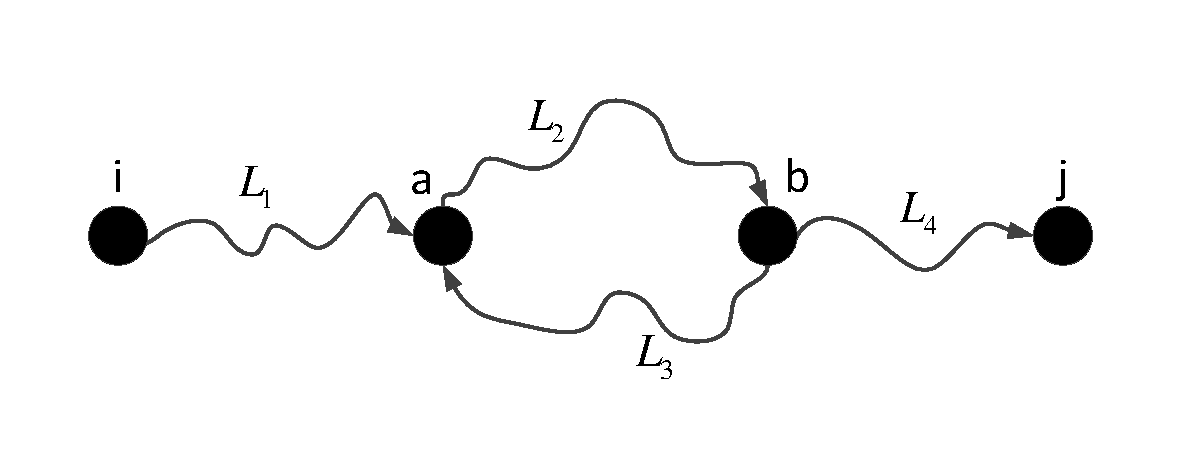
\includegraphics[width=1 \textwidth]{figures/circle.pdf}}
\end{center}
\caption{{\footnotesize{无环证明}}}
\label{prof}
\end{figure*}
\subsection{并行层次}
\subsection{并行动态规划算法}

上一节提出了动态规划模型,证明了算法的正确性,本节我们讨论这个动态规划算法在GPU上的并行设计框架,以及分层图和不同速率的并行层次设计。单个图上的动态规划的串行执行过程如下伪代码所示:
\begin{algorithm}[t]
\begin{algorithmic}[1]
\Require
点的入边集合$PreE$;
点的入点集合$PreN$;
源节点$s$;
\Ensure {最优代价数组$Price$;最优前驱节点数组$Pre$;}
\For {$k \in [1,W_{max}]$}
\For {$v \in V$}
\State {Price[s][v][k]=$\min\limits_{n \in PreN_v}{Price[s][n][k-1]+w_{nv}}$}
\State {Pre[i][j][k]=$\arg\min\limits_{n \in PreN_v}{Price[s][n][k-1]+w_{nv}}$}
\EndFor
\EndFor
\end{algorithmic}
\caption{{串行动态规划算法}}
\label{pda}
\end{algorithm}

算法循环$W_{max}$次,每一次循环中对每一个点进行对应的$Price$数组进行更新,而这些更新操作是相互独立的,所以,可以进行并行设计,对每一个点的$Price$ 数组更新操作开辟一个线程进行计算,这个线程遍历当前点的前驱边,寻找最优的那一条前驱边,这里的并行粒度只有图的点数$|N|$,但是考虑到不同个业务和不同的分层图上计算也是并行的,总的并行粒度为$|N|*|D|*|R|$,这样需要开辟大量的线程,充分利用GPU 上的SIMT计算资源。

下面考虑单个速率情况下的并行框架,如下图 \ref{DRK}所示,动态规划算法和BFS单个速率情况下的并行类似,只是BFS 那里的对每一条边并行的扩展操作被替换成了对每一个点并行的$Price$数组更新操作。
\begin{figure*}
\setlength{\belowcaptionskip}{-0.5cm}
\begin{center}
{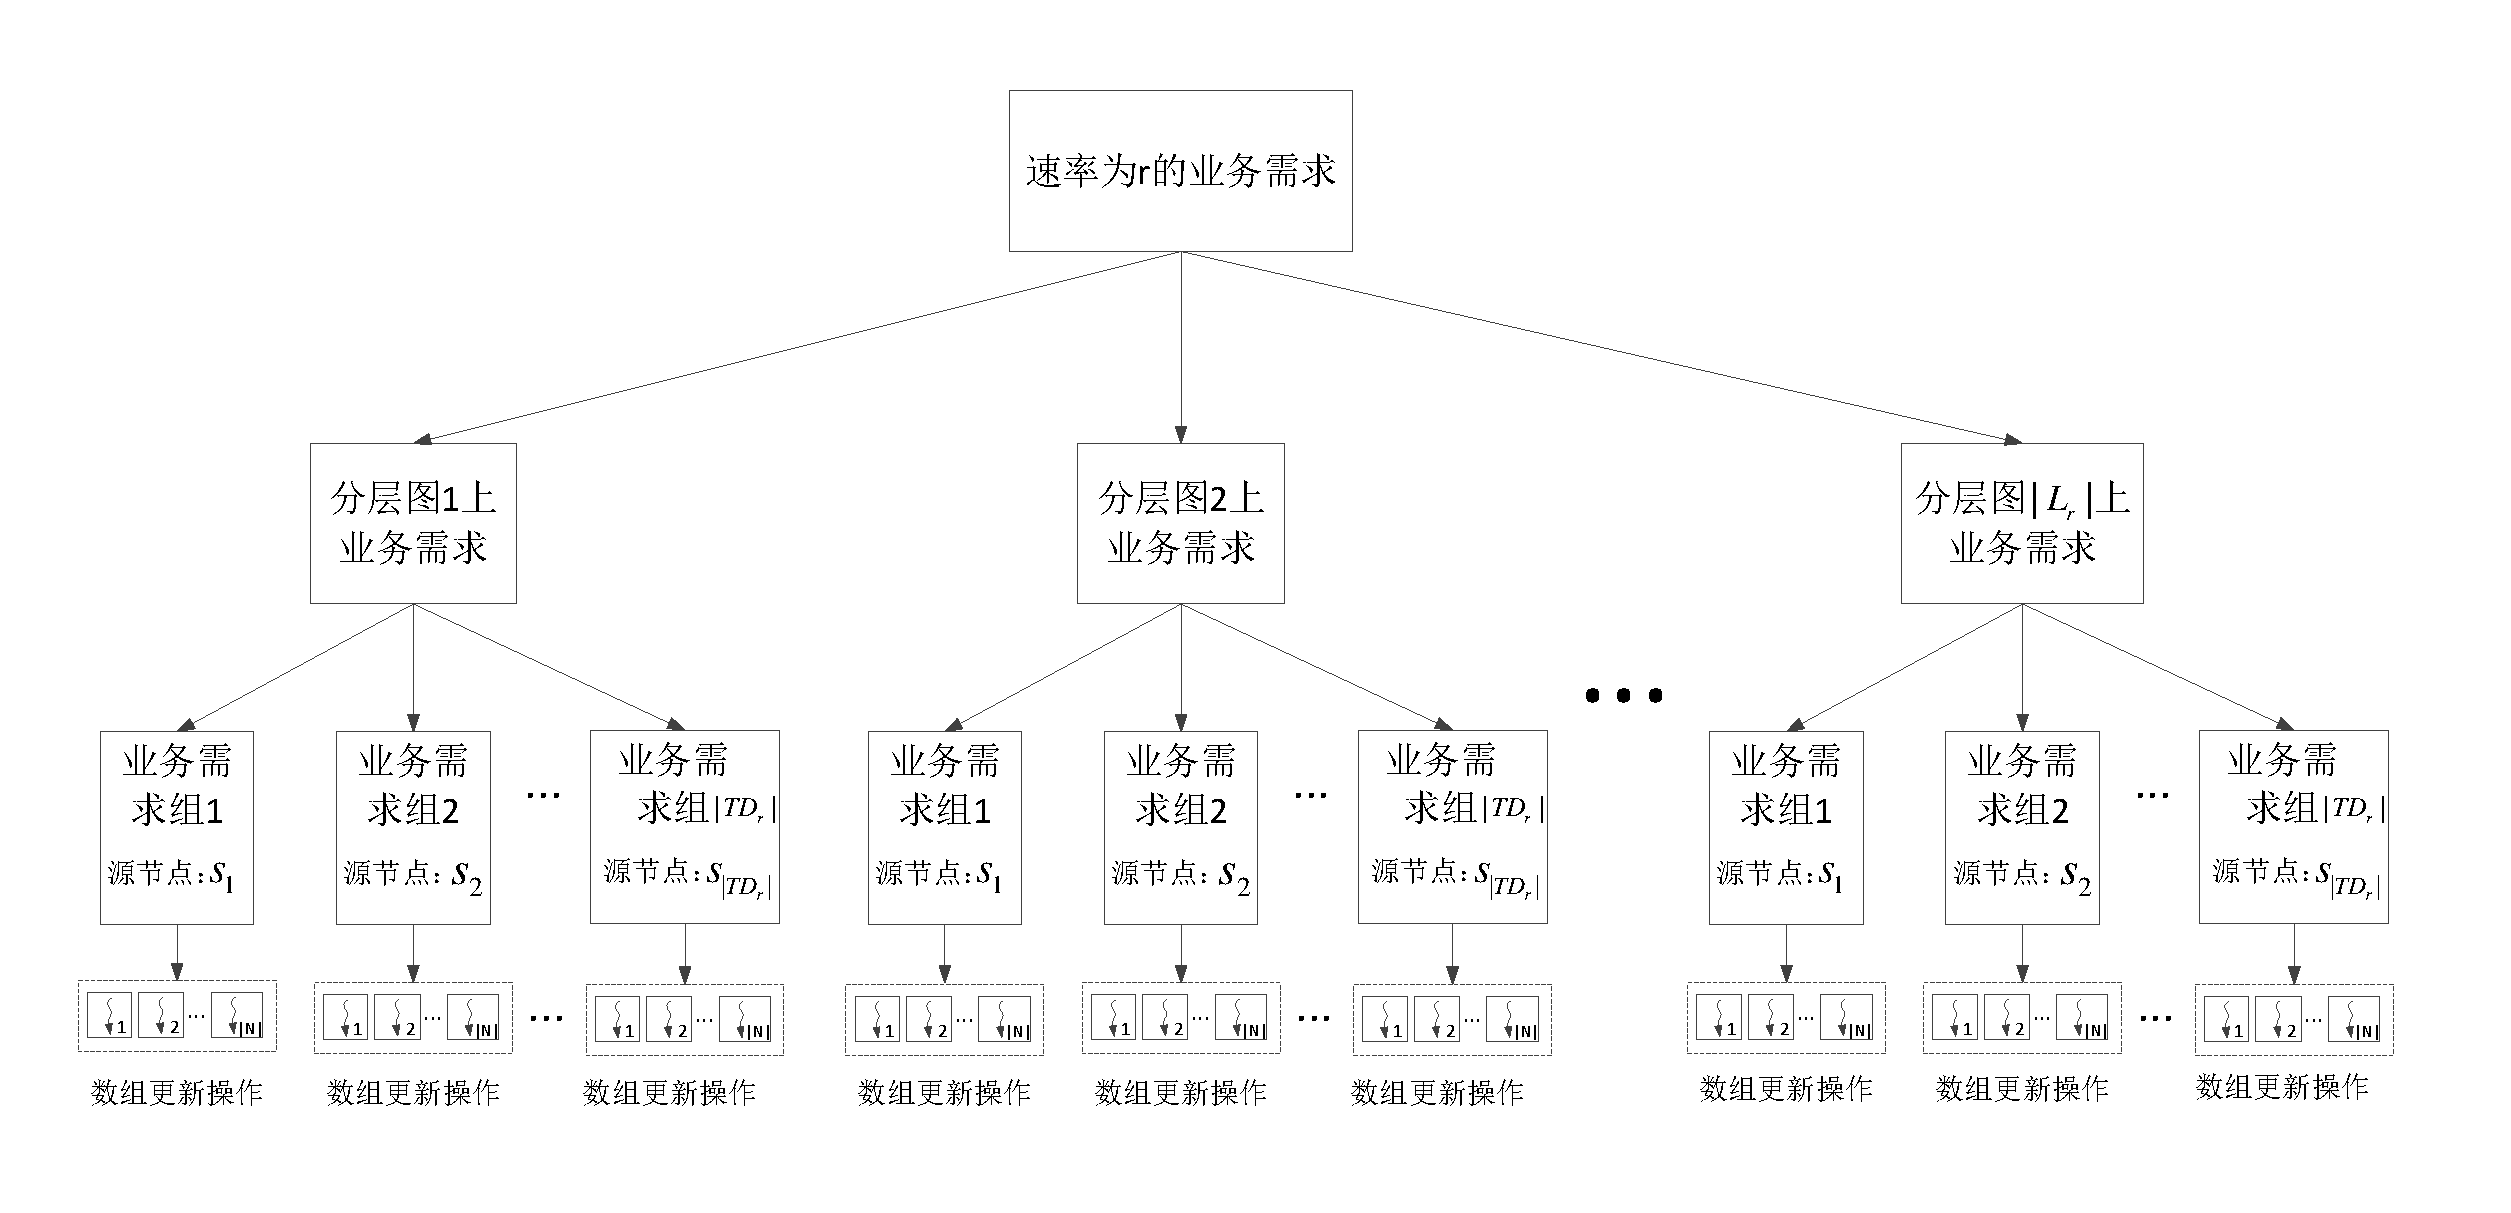
\includegraphics[width=1 \textwidth]{figures/DRK.pdf}}
\end{center}
\caption{{\footnotesize{动态规划并行示意图}}}
\label{DRK}
\end{figure*}

和BFS一样,对不同速率的业务,本文依然采用不同的流进行并行,其并行过程如下所示:
\begin{figure*}
\setlength{\belowcaptionskip}{-0.5cm}
\begin{center}
{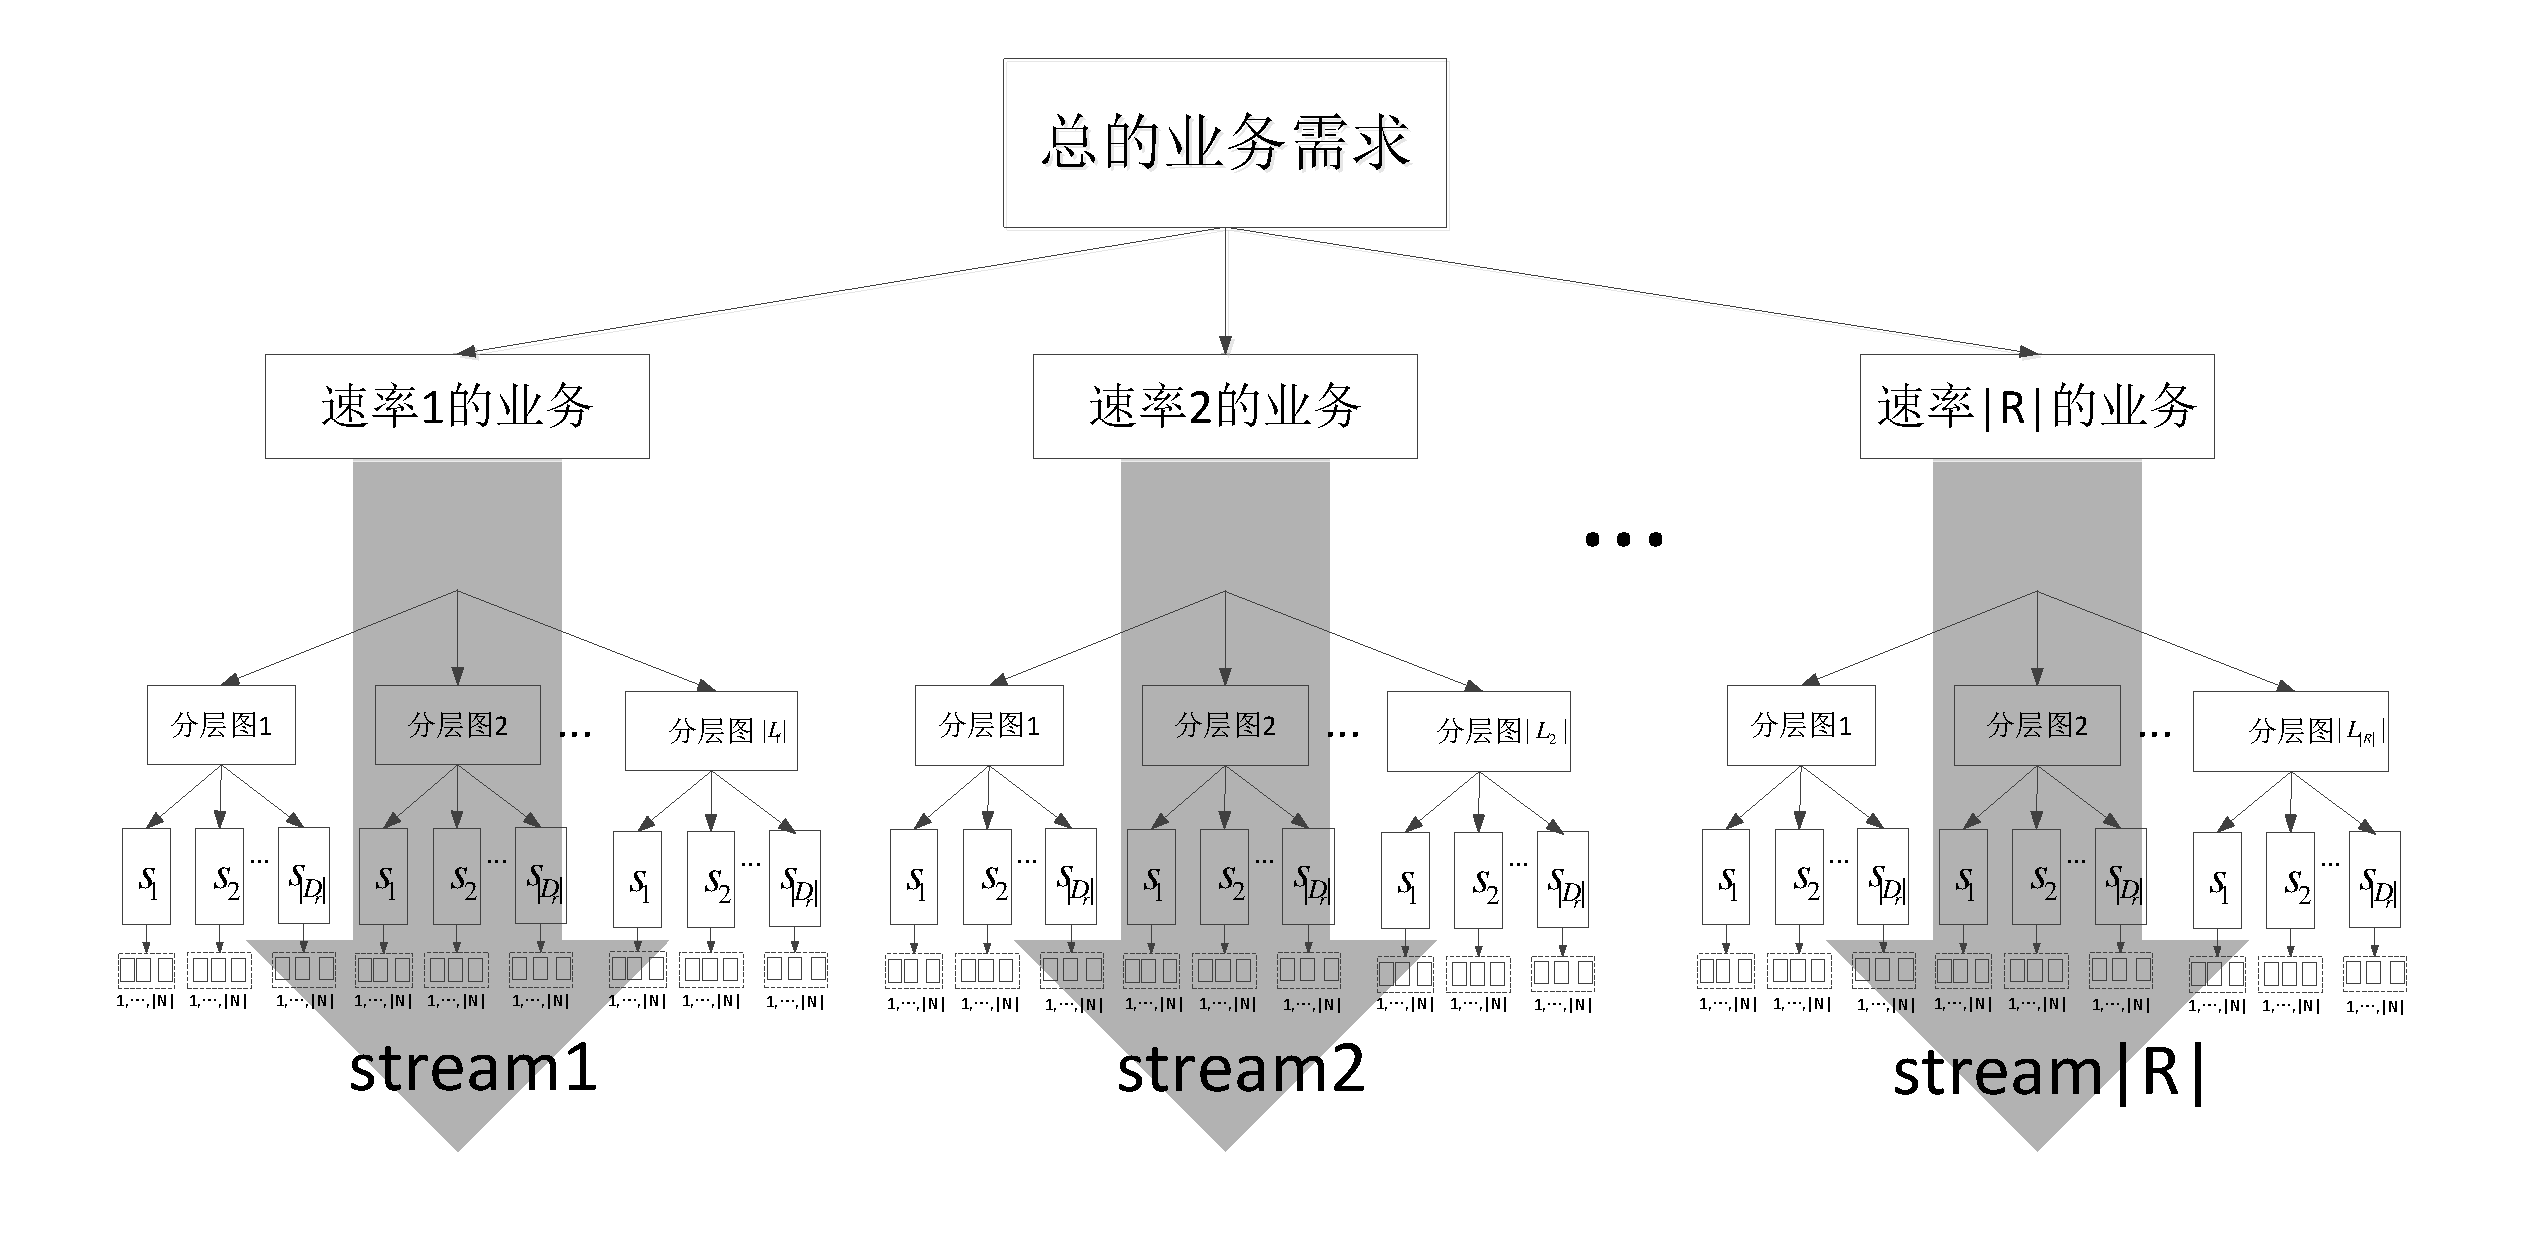
\includegraphics[width=1 \textwidth]{figures/BBK.pdf}}
\end{center}
\caption{{\footnotesize{动态规划流并行示意图}}}
\label{prof}
\end{figure*}
\subsection{GPU上kernel设计}
动态规划的GPU代码设计如下:
\begin{algorithm}[t]
\begin{algorithmic}[1]
\Function{kernel\_dynamic\_update}{$PE$,$rid$,$k$}
\State {$bid \leftarrow$ block ID}
\State {$tid \leftarrow$ thread ID}
\State {用$(bid,tid,rid)$ 映射到边点的标号$nid$}
\State {用$(bid,tid,rid)$ 映射到边源节点的标号$sid$}
\State {用$(bid,tid,rid)$ 映射到分层图标号$lid$}
\For {$e \in PE[lid][nid]$}
\If{$e.avalible>0$}
\If {$Price[lid][sid][nid][k]<Price[lid][sid][e.s][k-1]+e.weight$}
\State{$Price[lid][sid][nid][k]=Price[lid][sid][e.s][k-1]+e.weight$}
\State{$Pre[lid][sid][nid][k]=e.s$}
\EndIf
\EndIf
\EndFor
\EndFunction
\end{algorithmic}
\caption{kernel\_dynamic\_update}
\label{KernelDynamic}
\end{algorithm}
在$kernel\_dynamic\_update$中,输入$PE$是一个二维的集合数组,比如,$PE[2][3]$表示第2个分层图上点3 的入边集合。$Price$ 是预先分配的代价数组,他是一个三维数组,第一维表示当前代价数组对应的分层图标号,第二维度表示源节点,第三维度表示目的节点,第四维度表示路径的跳数,比如$Price[4][3][10][5]$=7 表示在第4个分层图上,点3到10的跳数为5的最优路径代价为7,初始时,当跳数等于0 时,除了源节点代价被初始化为0 之外,其他的距离都被初始化为无穷大。
$Pre$数组是前驱数组用以记录前驱信息来恢复路径,$Pre$数组和$Price$数组一样,是一个四维数组,$Pre[4][3][10][5]$=50 表示在第4 个分层图上,点3 到10 的跳数为5的最优路径的前驱节点(也就是路径上的倒数第二个点)为点50。$rid$表示当前kernel 负责的计算的业务速率标号,他是区分不同流的标记,$rid$ 不同表示执行kernel的流不同。$k$ 表示当前扩展的层数,也就是跳数。算法开始时先进行一系列映射操作,将线程映射到点标号$eid$,当前所在分层图标号$lid$,以及源节点标号$sid$,映射完成后就可以进行Price数组的更新了,也就是要去寻找最优的入边,算法遍历点的所有入边,由于动态情况下,边的可用状态可能发生变化,找到边之后,需要判断这条边是否可用,如果不可用则跳过这条边,反之,就判断更新条件是否成立($Price[lid][sid][nid][k]<Price[lid][sid][e.s][k-1]+e.weight$),如果条件成立则说明这条入边比之前的要好,经过这条边到达当前点的路径代价更小,所有要更新Price数组,同时为了后面恢复路径需要记录前驱信息在数组$Pre$中。
\begin{algorithm}[t]
\begin{algorithmic}[1]
\Require
业务需求集合$TD$;
各个分层图前驱链路集合$PE$;
\Ensure {业务需求的最短路径集合$P$}
\State {将业务根据速率和源节点重新组合成业务分组集合$D$}
\For {$D_r \in D$}
\For {$d_{rs} \in D_r$}
\For {$l \in L_r$}
\For {$v \in V$}
\If {$v==s$}
\State {$Price[l][s][v][0]\leftarrow$ 0}
\Else
\State {$Price[l][s][v][0]\leftarrow \infty $}
\EndIf
\State {$Pre[l][s][v][0]\leftarrow -1 $}
\EndFor
\EndFor
\EndFor
\EndFor
\State {新建$|R|$个流,组成集合$S$}
\State {$k \leftarrow$ 1}
\While{$k<=W_{max}$}
\For{r in R}
\State {在流$S_r$上发射 kernel\_dynamic\_update($PE$,$rid$,$k$)}
\EndFor
\State{k=k+1}
\EndWhile
\State {根据前驱数组$Pre$重建路径,然后把路径加入到集合$P$}
\end{algorithmic}
\caption{{并行动态规划的计算}}
\label{ParaSPC}
\end{algorithm}

算法开始时先将业务按照速率的不同进行划分,再将业务按照源节点的不同划分成不同的业务组集合$D$,比如,$D_r \in D$ 表示速率为$r$ 的业务组集合,$d_{rs} \in D_r$ 表示速率为$r$的源节点标号为$s$的业务组。划分好业务组之后,就开始初始化代价数组,将速率对应的所有分层图上的跳数为0的源节点代价初始化为0,这是一个三层的for 循环,第一层遍历速率标号,第二层遍历源节点标号,第三层遍历速率所对应的分层图标号;初始化$Price$数组后,在发射kernel之前需要先新建$|R|$ 个GPU 流,不同的流将对不同速率的业务进行计算。$k$为扩展的跳数标记,开始时$k$初始化为1。while循环中进行扩展操作,其中$W_{max}$ 为跳数限制,最大跳数不能超过$W_{max}$,所以最多只能循环$W_{max}$ 次。while循环中for 循环用来发射不同的流,因为发射不同流的kernel 是异步操作,for循环不会去等待上kernel结束了才去执行下一个kernel,所以可以认为所有kernel 都是同时间发射的。
\section{实验仿真分析}

实验仿真中我的采用两个速率的链路,假设已知两种速率的业务的大致比例为1:3,于是,我们初始时为速率1 的业务分配20 层的频谱连续分层网络,速率2 的业务分配60 层的频谱连续的分层网络。我们假设对业务的加入服从泊松过程,一共产生了1000个加入事件,每个加入事件间的时间间隔服从均值为4的负指数分布,当加入事件到达时,产生速率1的业务为$d_1$ 个,范围为$[200-400]$, 产生速率为2的业务$d_2$ 个,其中$d1$ 为2|N|到4|N|中的随机值,$d_2$为6|N| 到12|N| 之间的随机值。初始时网络的节点为$N$, 平均度数为$4$。 每个业务的服务时间满足均值为$ST$ 的负指数分布。我们在不同$ST$ 下进行仿真,观察各个算法在不同服务压力下的权值变化,跳数变化和阻塞率变化情况。
\subsection{对比算法}

为了说明PRORSA对路径代价和网络阻塞率带来的优化效果,我们将PRORSA/SRORSA和不进行路径优化的贪心算法进行比较,我们称这个算法为GRSA(Greedy ),算法的执行伪代码如下 \ref{ParaSPC}所示:
\begin{algorithm}[t]
\begin{algorithmic}[1]
\Require
业务需求集合$TD$;
分层图集合$G$;
\Ensure {业务需求的路径集合$P$;阻塞的需求集合$Z$}
\For{$r \in R$}
\State{$flag \leftarrow 0$ }
\For{$TD_r \in TD$}
\State{把$TD_r$中的业务按照其在第一层分层图上的路径跳数进行排序}
\For{$d \in TD_r$}
\For{$g \in G_r$}
\If{在分层图g上存在业务$d$的合法路径$p$}
\State{更新分层图g上的链路占用情况}
\State{把路径p加入到结果路径集合$P$中}
\State{$flag \leftarrow 1$}
\State{\bfseries break}
\EndIf
\EndFor
\If{$flag=0$}
\State{把业务$d$加入阻塞集合$Z$中}
\EndIf
\EndFor
\EndFor
\EndFor
\end{algorithmic}
\caption{{贪心的分层RSA算法}}
\label{ParaSPC}
\end{algorithm}

当业务到达时,GRSA先在第一层对所有业务求最短路径,得到一个路径跳数值,按照这个跳数值对业务进行排序,这是为了优先加入较短的业。然后逐层去寻找是否能够把业务加入到网络中,如果能加入到当前层中,那么就更新当前层上的相应链路的占用情况,如果没有找到合法路径,就在下一层进行搜寻。如果所有层都无法加入这个业务,那么业务就被阻塞,加入到阻塞集合。
\subsection{无权图下的仿真结果}
\subsubsection{路径优化分析}

在无权图下,优化目标是最小化路径的跳数,图 \ref{B5H}到图 \ref{B40H}表示了无权图下的跳数优化结果,我们把PRORSA和SRORSA的优化结果与贪心算法GRSA 的算法权值优化结果进行比较,图中的横坐标表示业务到达的次数,我们一共产生了1000个加入事件,当网络状况较好的时候,比如,平均服务时间为$ST=5$ 时,PRORSA/SRORSA的平均跳数为2.73, 而GRSA 的平均跳数为3.73,平均跳数要少一跳左右,这样PRORSA/SRORSA可以大大的减小对网络资源的占用。随着平均服务时间$ST$的增加,PRORSA/SRORSA和GRORSA的平均跳数都有所增加,但是PRORSA/SRORSA 的增幅较小,从$ST=5$ 时的平均跳数为2.73增加到$ST=40$时的平均跳数为2.82,也就是说不管在网络空闲还是繁忙的情况下,PRORSA/SRORSA都能够很好得优化跳数。而GRSA的跳数随着$ST$的增加而大幅增加从$ST=5$ 时的平均3.75增加到$ST=40$时的平均4.2。
\begin{figure*}
\setlength{\belowcaptionskip}{-0.5cm}
\begin{center}
{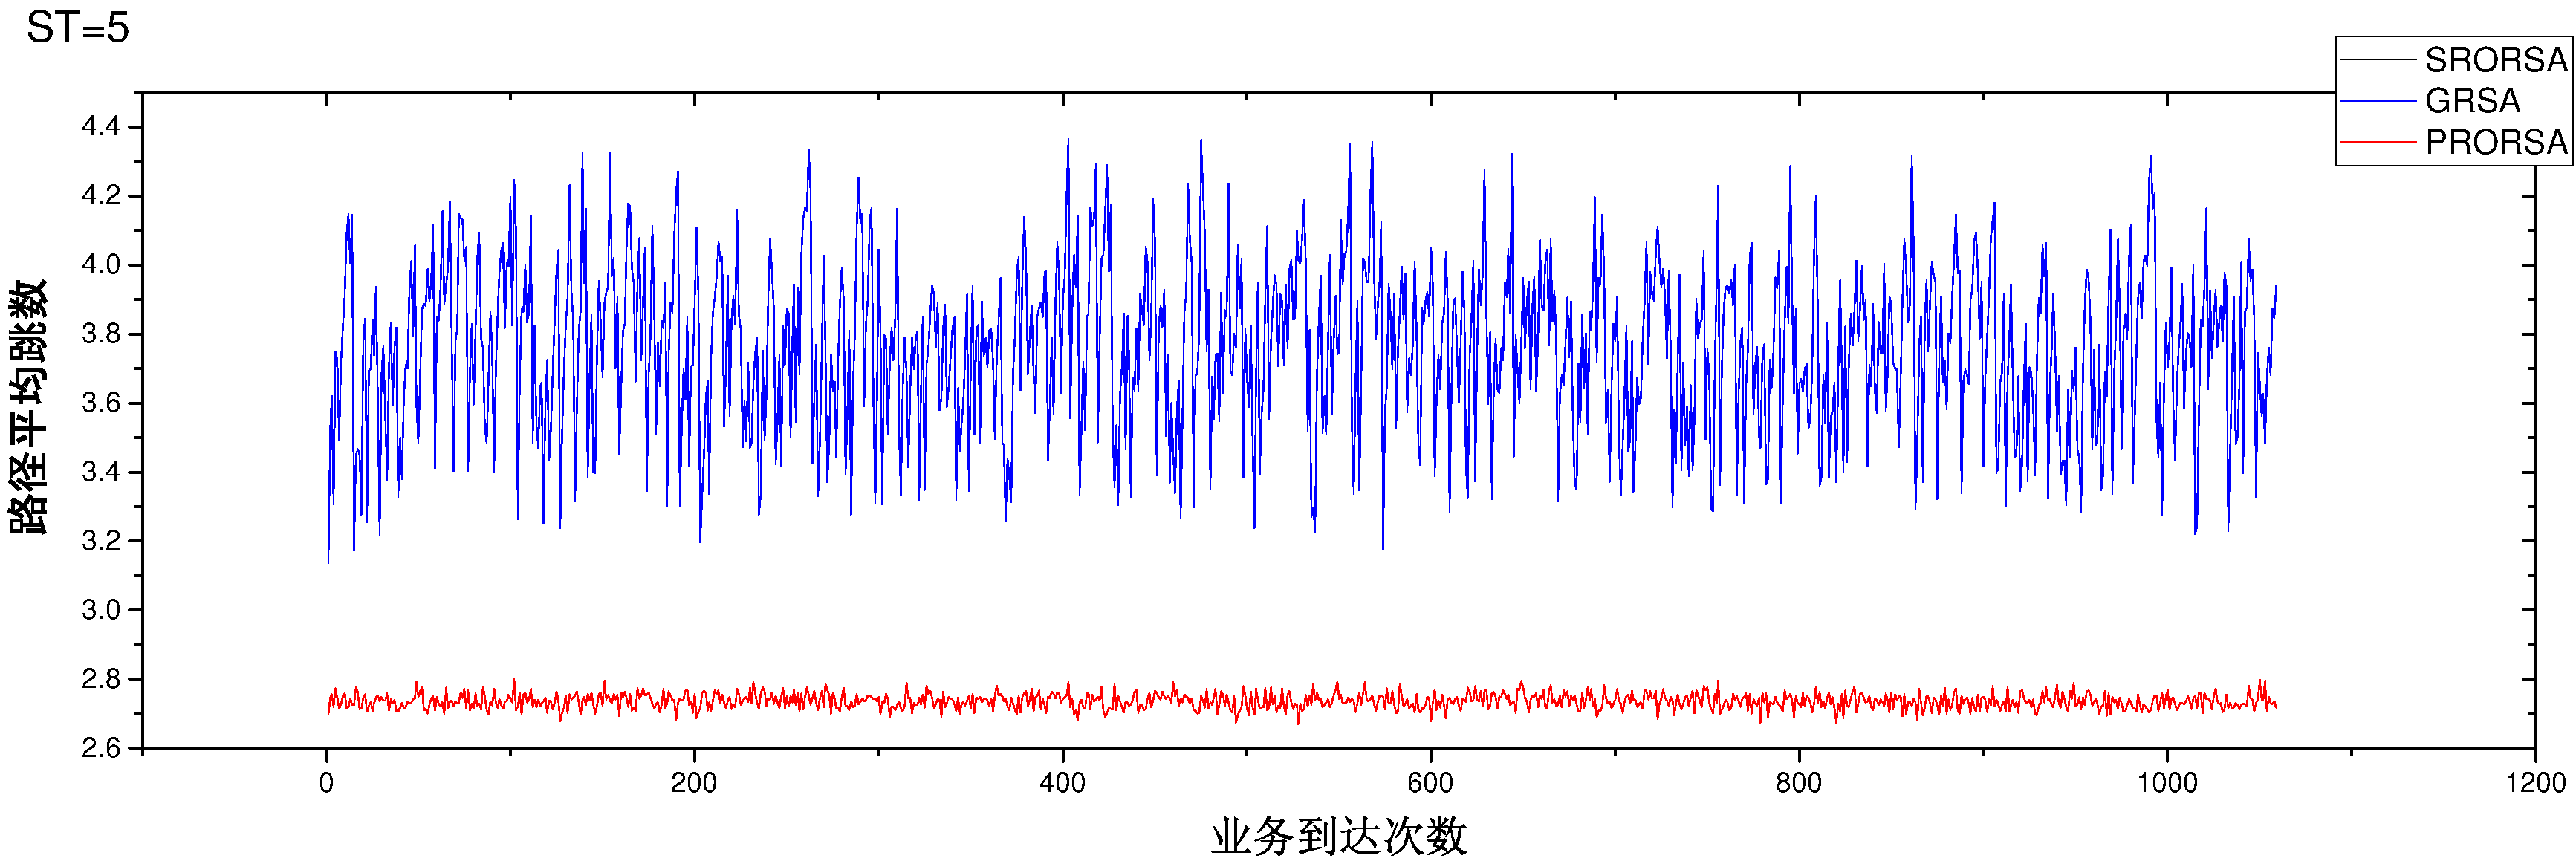
\includegraphics[width=1 \textwidth]{figures/B5H.pdf}}
\end{center}
\caption{{\footnotesize{无权图路径跳数对比(ST=5)}}}
\label{B5H}
\end{figure*}
\begin{figure*}
\setlength{\belowcaptionskip}{-0.5cm}
\begin{center}
{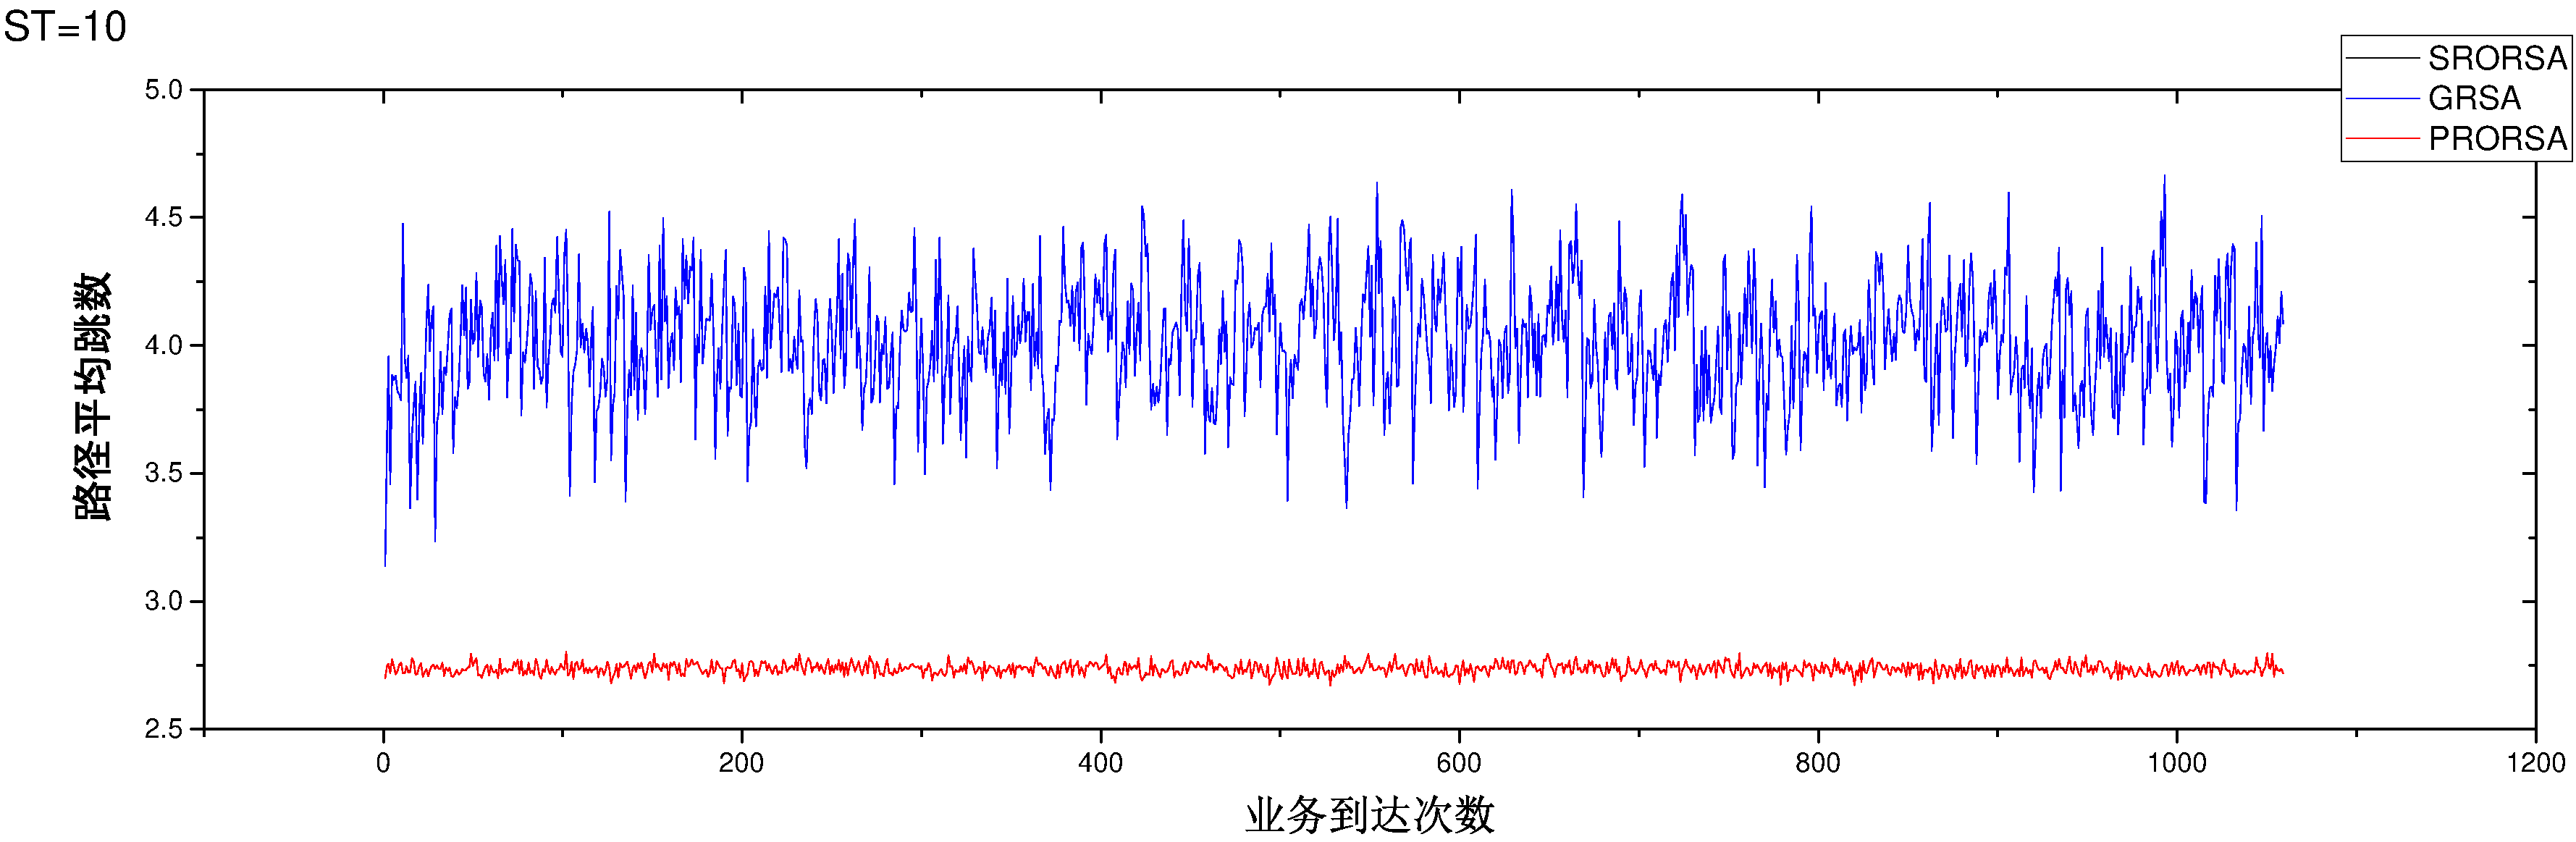
\includegraphics[width=1 \textwidth]{figures/B10H.pdf}}
\end{center}
\caption{{\footnotesize{无权图路径跳数对比(ST=10)}}}
\label{B10H}
\end{figure*}
\begin{figure*}
\setlength{\belowcaptionskip}{-0.5cm}
\begin{center}
{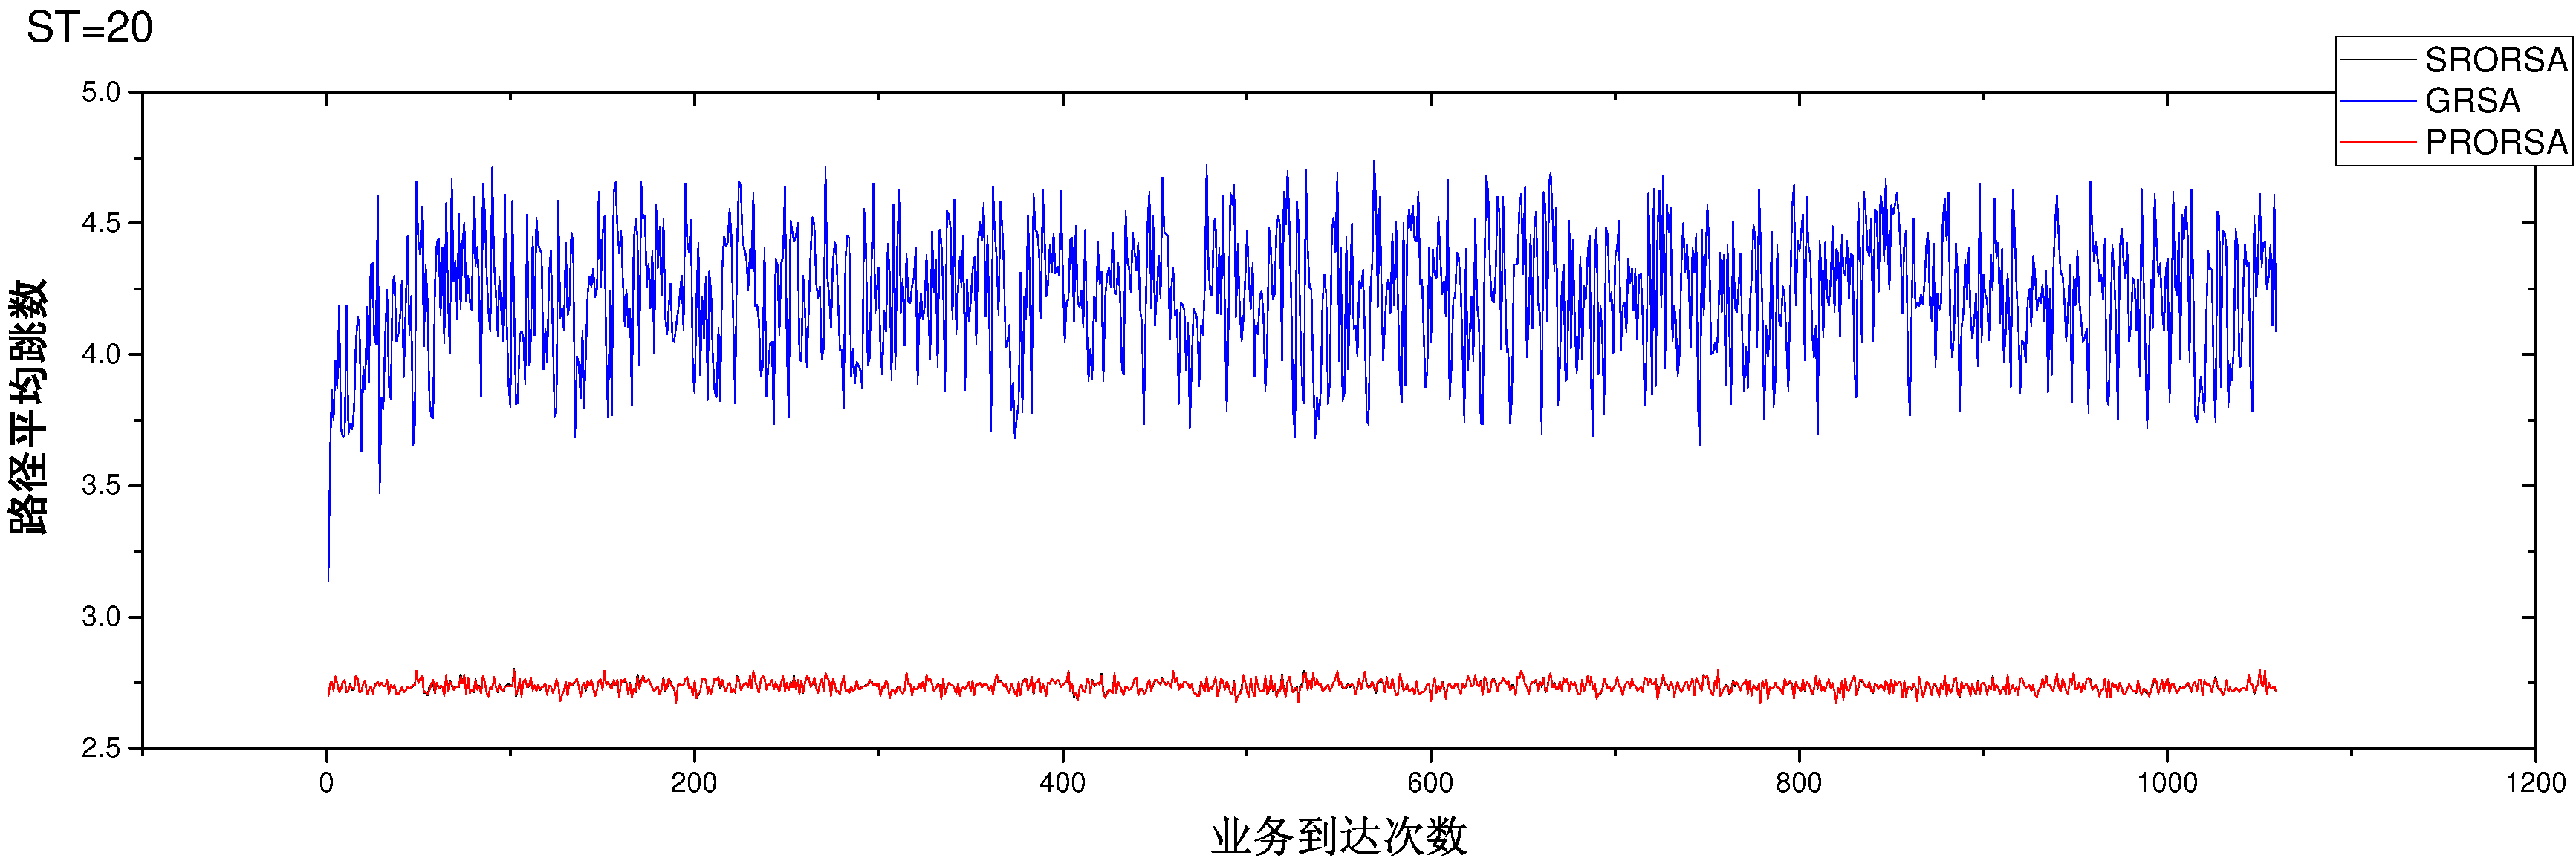
\includegraphics[width=1 \textwidth]{figures/B20H.pdf}}
\end{center}
\caption{{\footnotesize{无权图路径跳数对比(ST=20)}}}
\label{B20H}
\end{figure*}
\begin{figure*}
\setlength{\belowcaptionskip}{-0.5cm}
\begin{center}
{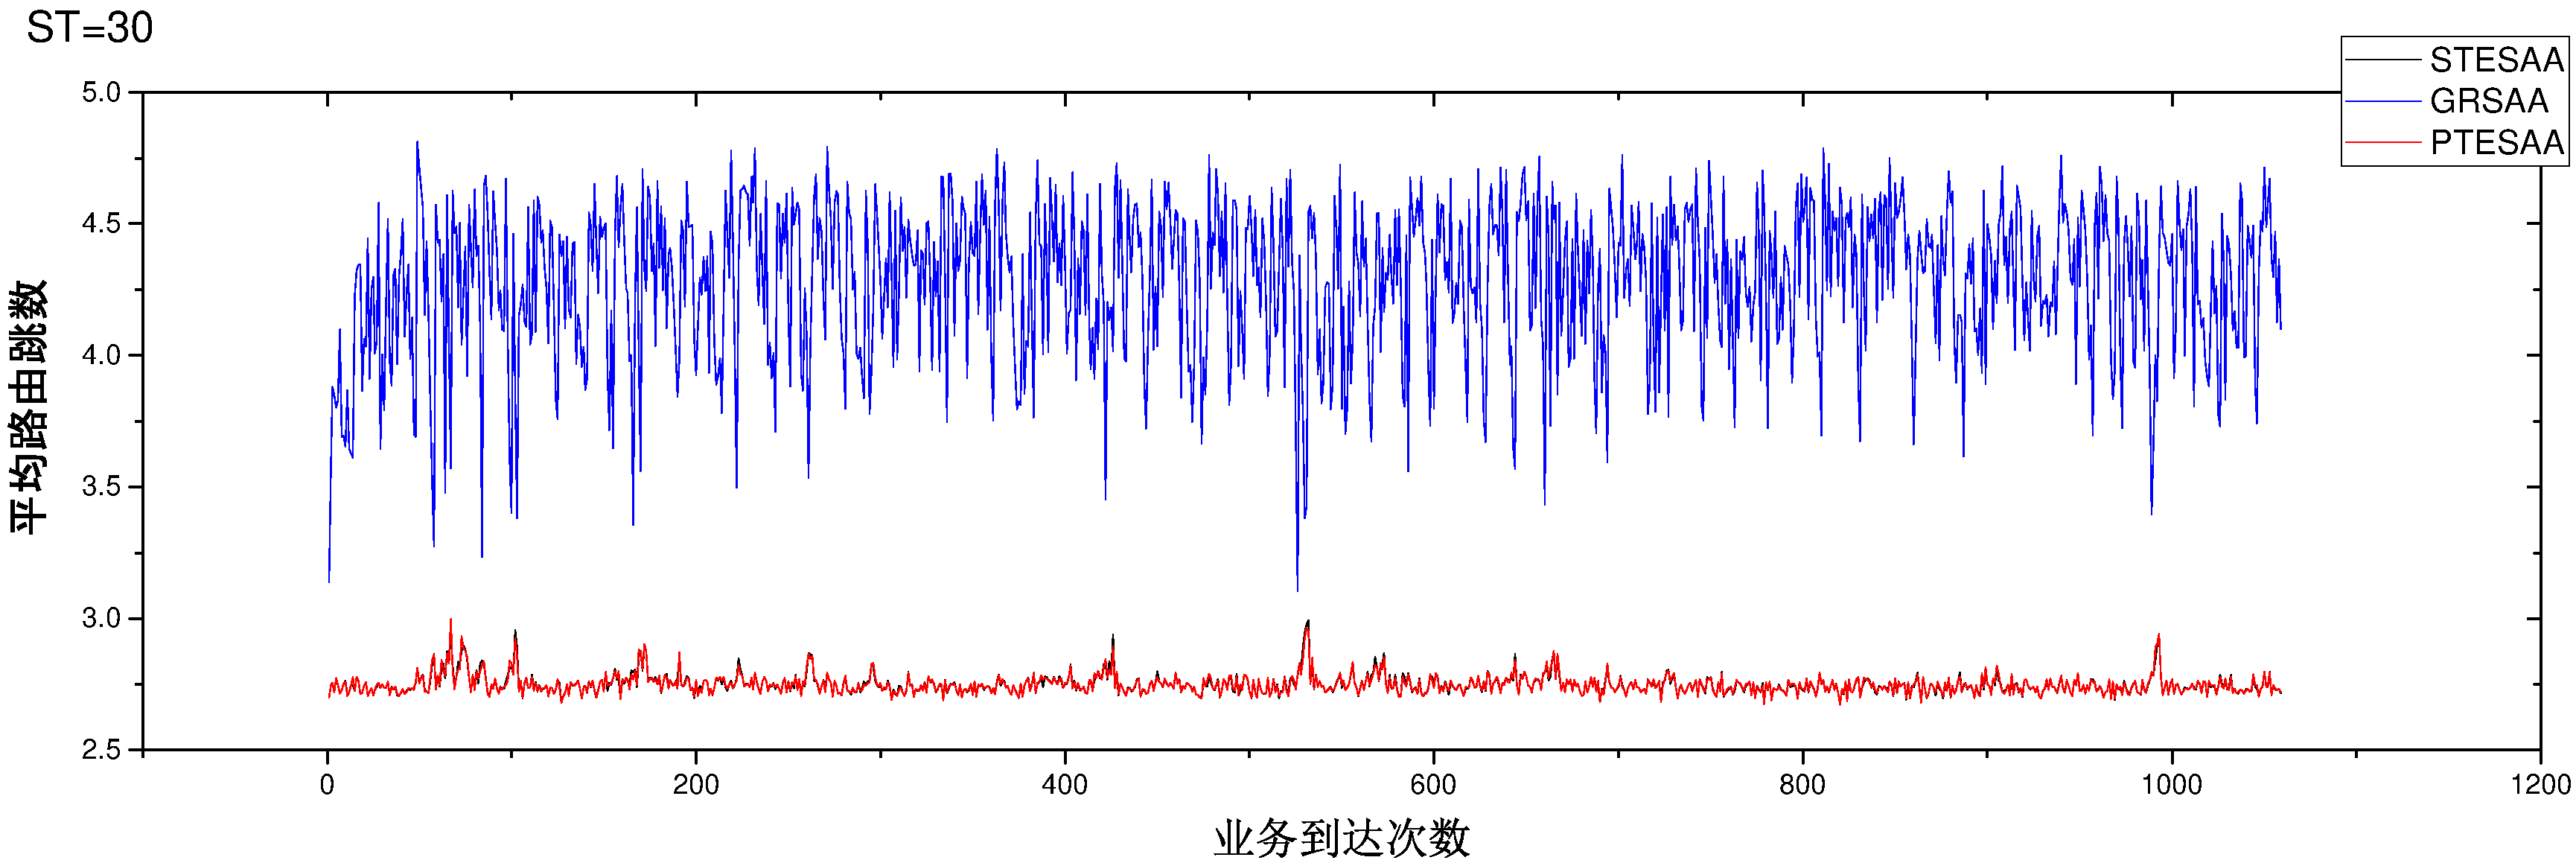
\includegraphics[width=1 \textwidth]{figures/B30H.pdf}}
\end{center}
\caption{{\footnotesize{无权图路径跳数对比(ST=30)}}}
\label{B30H}
\end{figure*}
\begin{figure*}
\setlength{\belowcaptionskip}{-0.5cm}
\begin{center}
{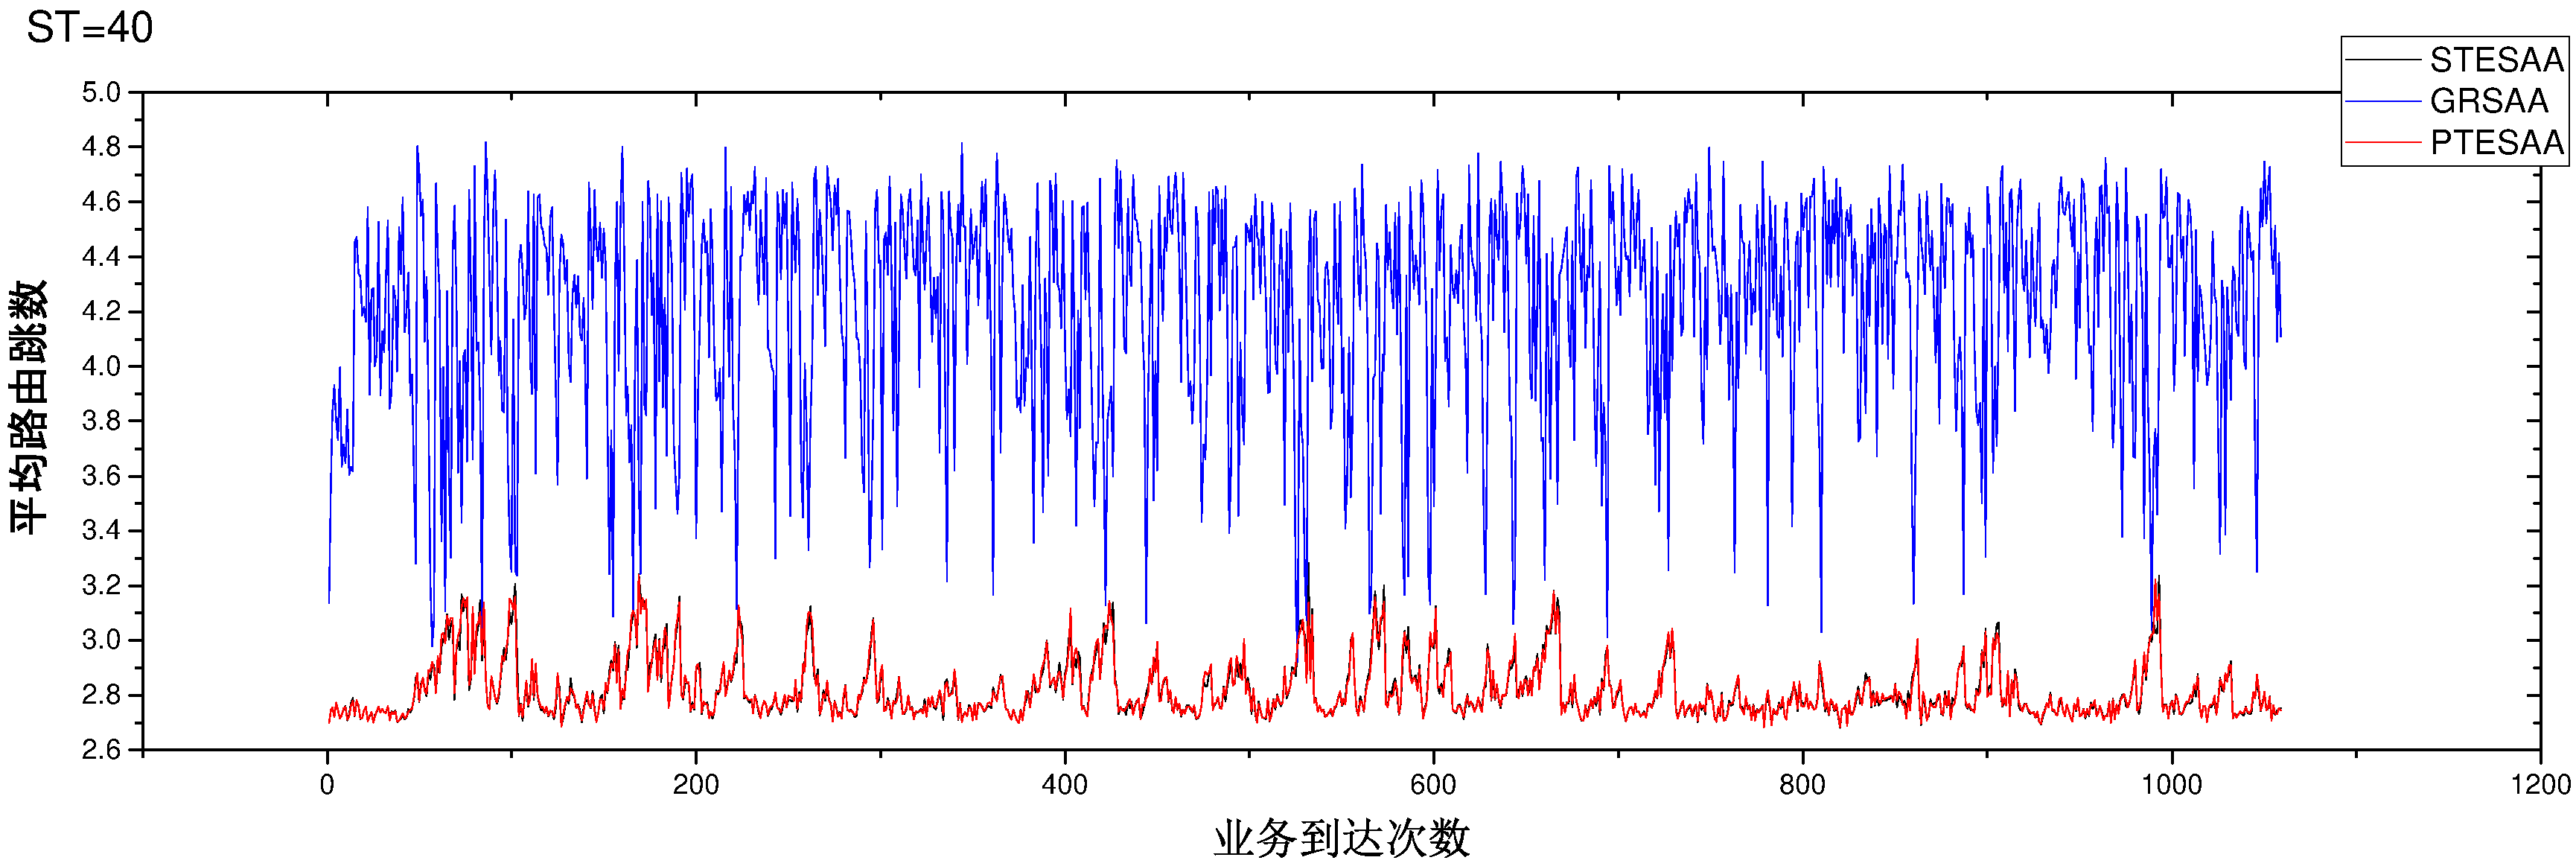
\includegraphics[width=1 \textwidth]{figures/B40H.pdf}}
\end{center}
\caption{{\footnotesize{无权图路径跳数对比(ST=40)}}}
\label{B40H}
\end{figure*}
\subsubsection{时间分析}

图 \ref{B5T}到图 \ref{B40T}展示了在不同平均服务时间$ST$下的各种算法的计算时间,当$ST=5$时,我们可以看到通过GPU加速的PRORSA的计算时间是SPROA 的计算时间的1/4,而实际上备选路径部分的GPU加速达到了7-8 倍,但是由于步骤二的快速路径选择过程也需要消耗一部分时间,这部分时间不能进行GPU加速,实际上PRORSA的大部分算法时间花在了步骤二的路径选择上,所以使得总体的加速比下降为4倍左右。我们发现由于PRORSA的波动幅度比SRORSA的波动幅度小很多,这是因为SRORSA的大部分时间花在计算备选路上,备选路径的计算量随着业务数量和网络链路的占用情况变化较大,而PRORSA的计算量花在步骤二上,计算量变化较小。GRSA的计算时间略高于PRORSA的计算时间,而且GRSA的波动幅度很大,不够平稳,这是因为GRSA贪心策略占用链路资源过多,容易造成分层图链路的碎片化,使得计算量变化较大。
观察到随着$ST$的变化PRORSA的对SRORSA的加速比逐渐下降,这是因为随着网络压力的增加,可用链路变少,使得SRORSA的备选路径计算复杂度下降,PRORSA加速优势变小。另外,随着$ST$的增加,PRORSA 和SRORSA的时间波动幅度增加,这是因为由于链路繁忙,使得大量业务不能一次性加入,步骤二到步骤一之间的循环次数增加,使得某些业务到达点的业务需要多次的循环,计算时间变长,从而拉大了时间变化幅度。
\begin{figure*}
\setlength{\belowcaptionskip}{-0.5cm}
\begin{center}
{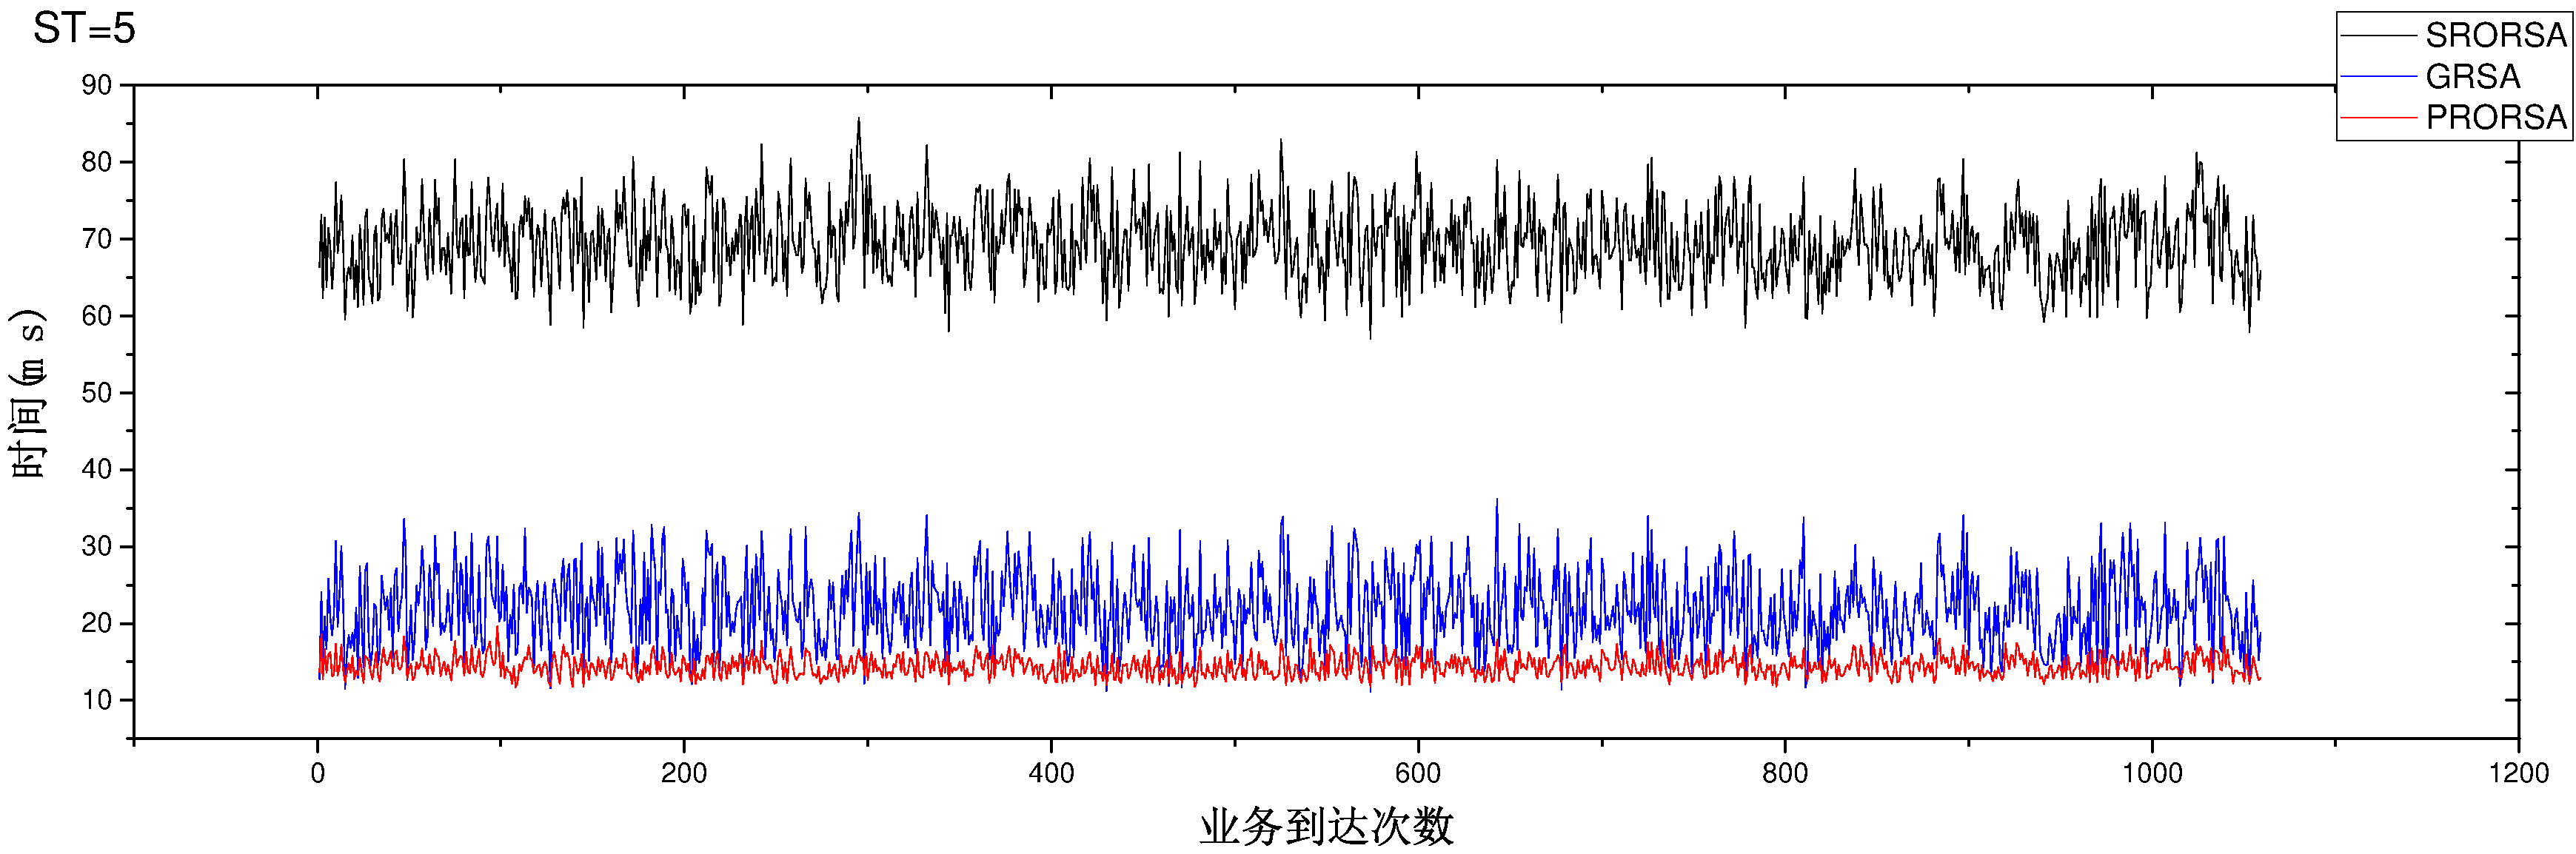
\includegraphics[width=1 \textwidth]{figures/B5T.pdf}}
\end{center}
\caption{{\footnotesize{无权图时间对比(ST=5)}}}
\label{B5T}
\end{figure*}
\begin{figure*}
\setlength{\belowcaptionskip}{-0.5cm}
\begin{center}
{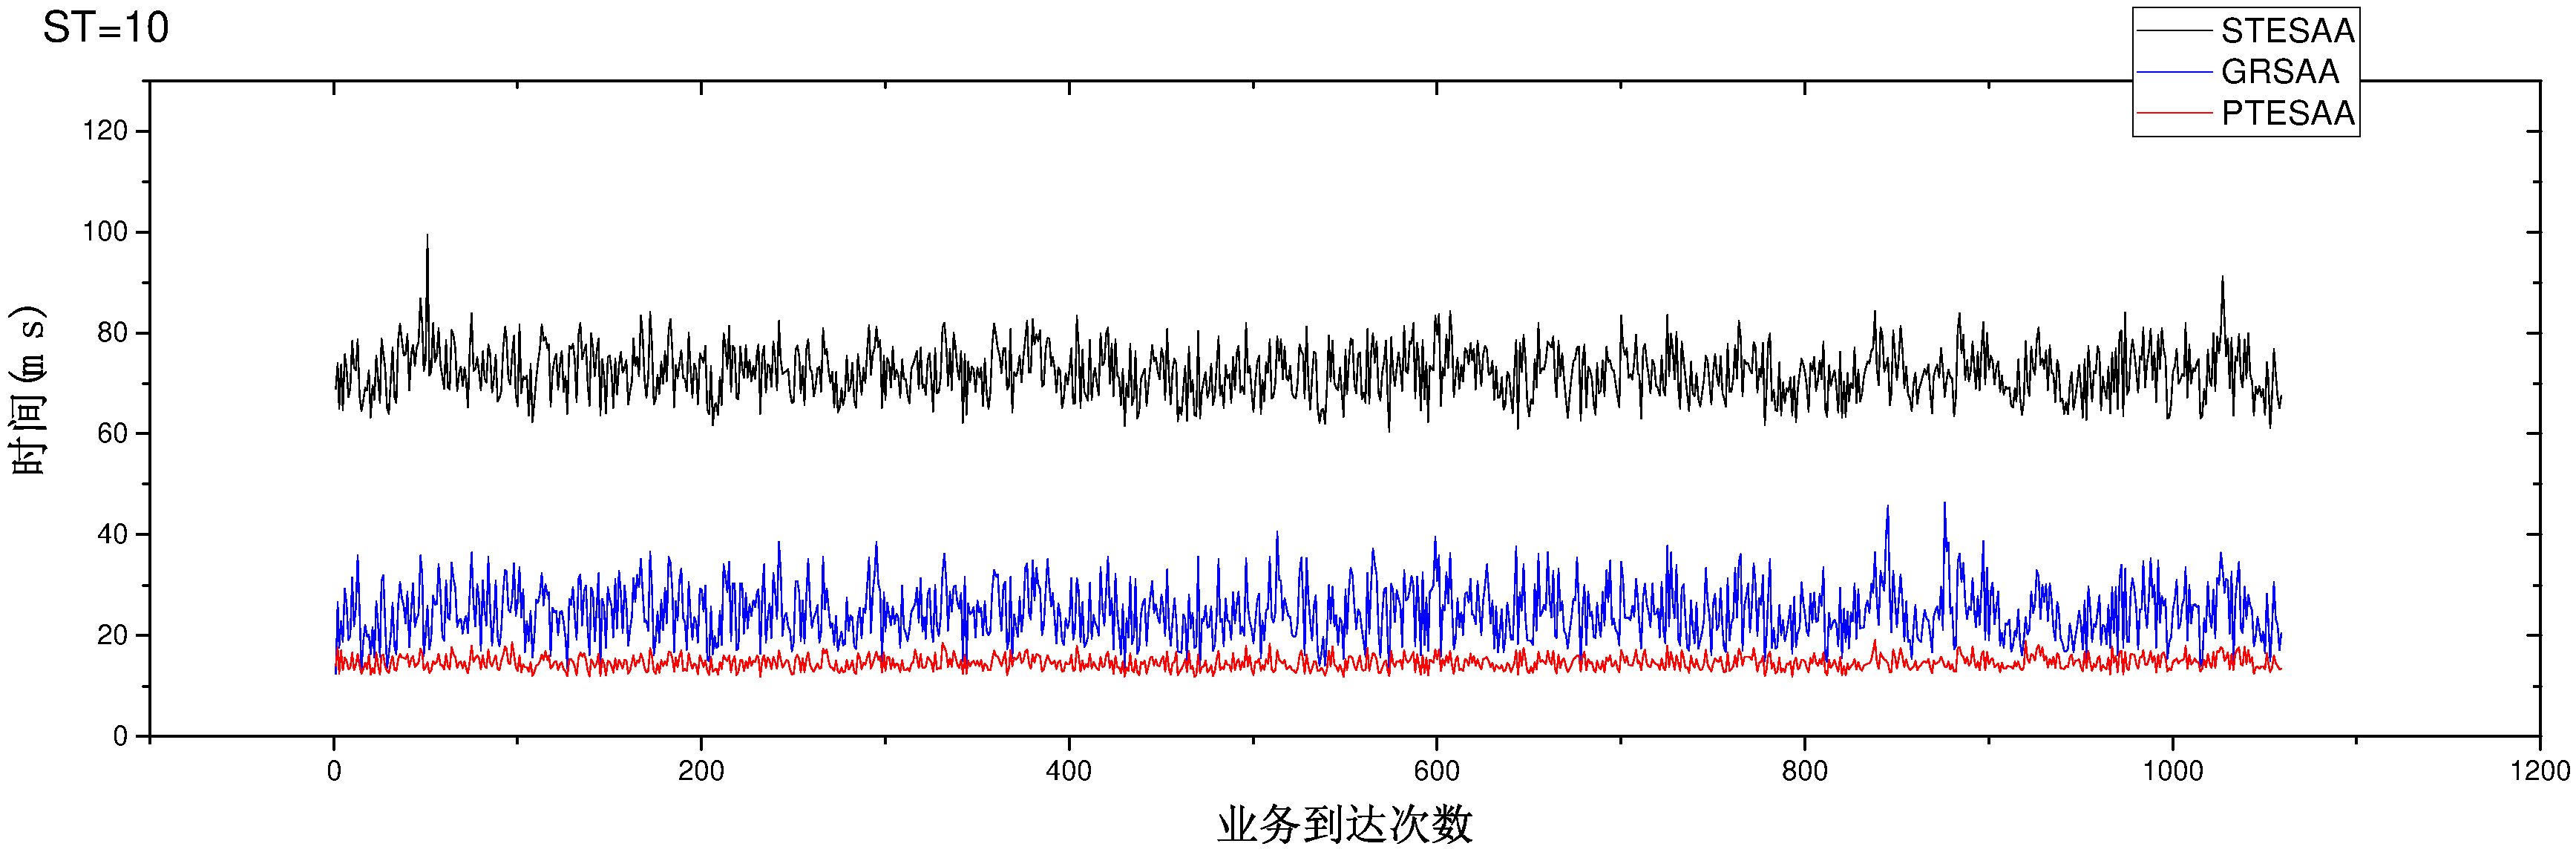
\includegraphics[width=1 \textwidth]{figures/B10T.pdf}}
\end{center}
\caption{{\footnotesize{无权图时间对比(ST=10)}}}
\label{B10T}
\end{figure*}
\begin{figure*}
\setlength{\belowcaptionskip}{-0.5cm}
\begin{center}
{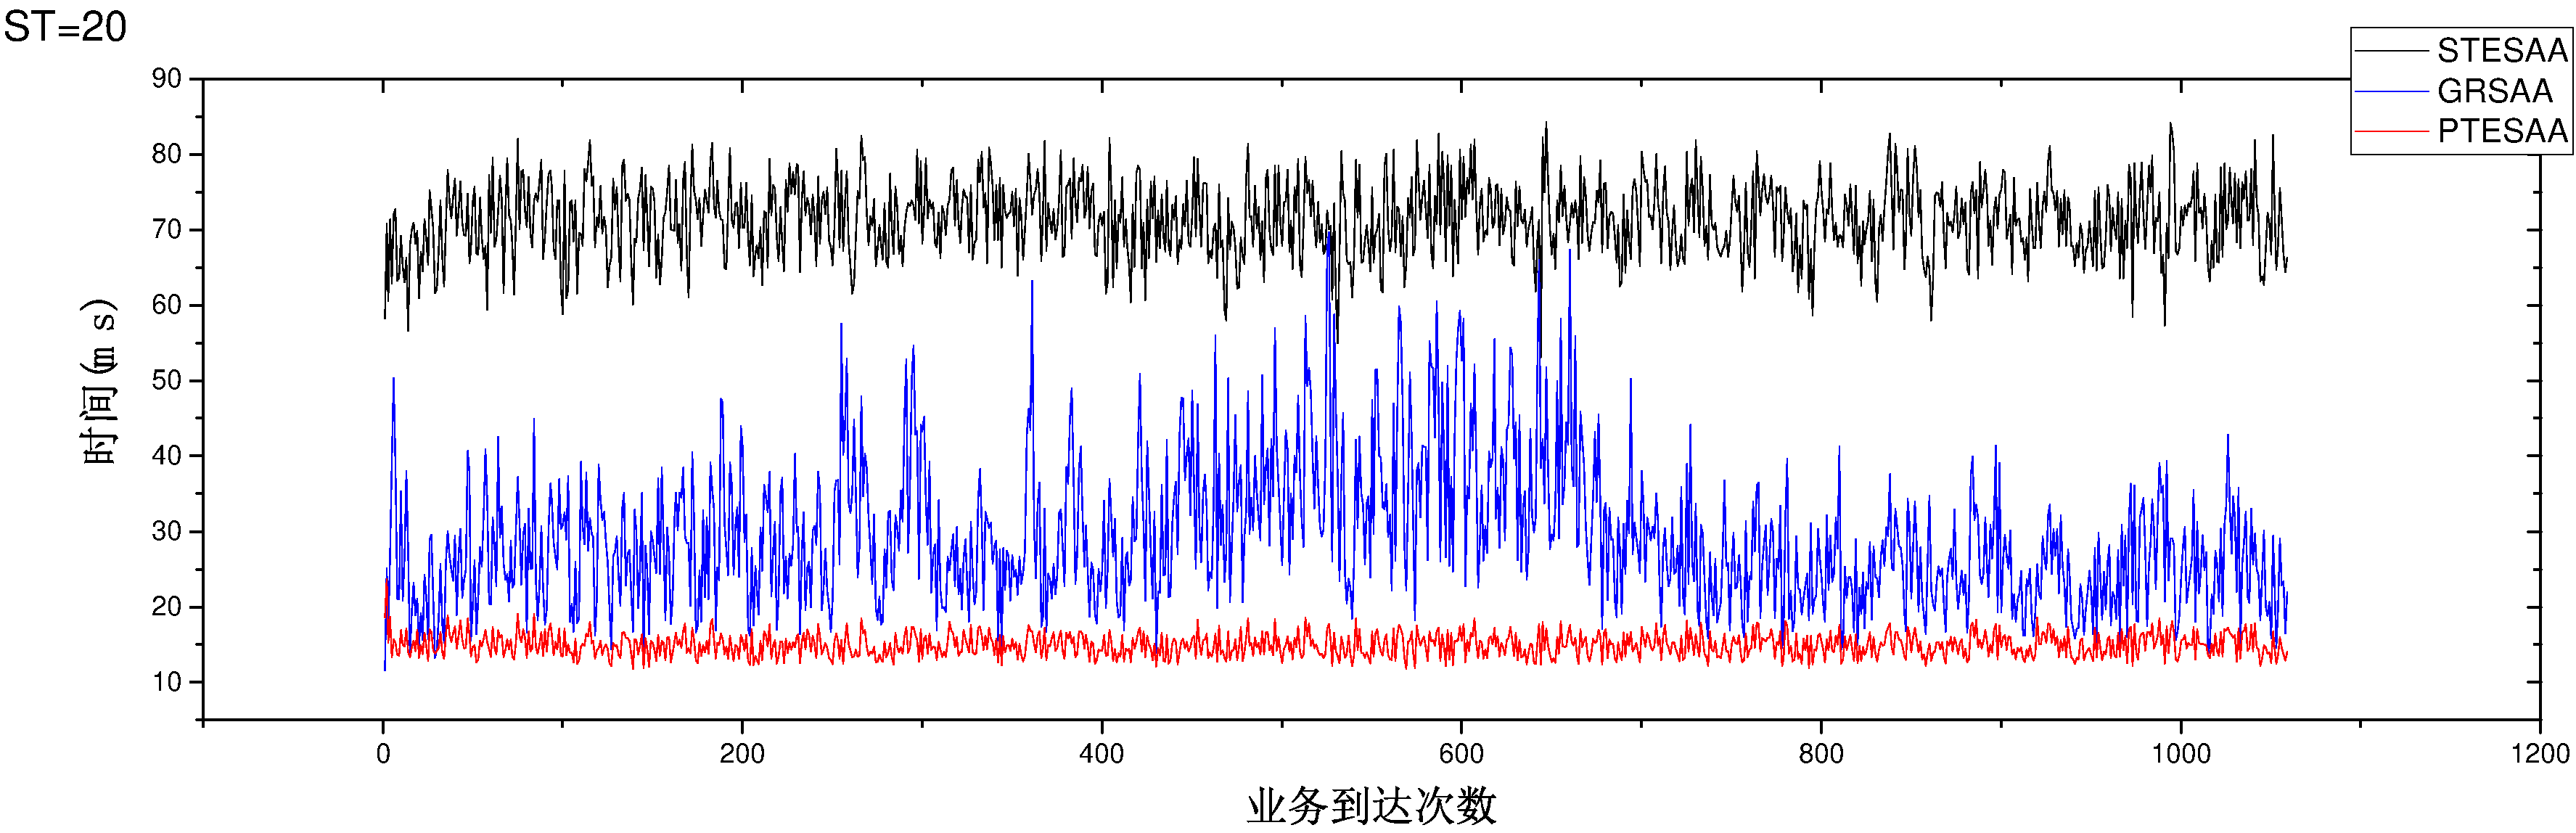
\includegraphics[width=1 \textwidth]{figures/B20T.pdf}}
\end{center}
\caption{{\footnotesize{无权图时间对比(ST=20)}}}
\label{B20T}
\end{figure*}
\begin{figure*}
\setlength{\belowcaptionskip}{-0.5cm}
\begin{center}
{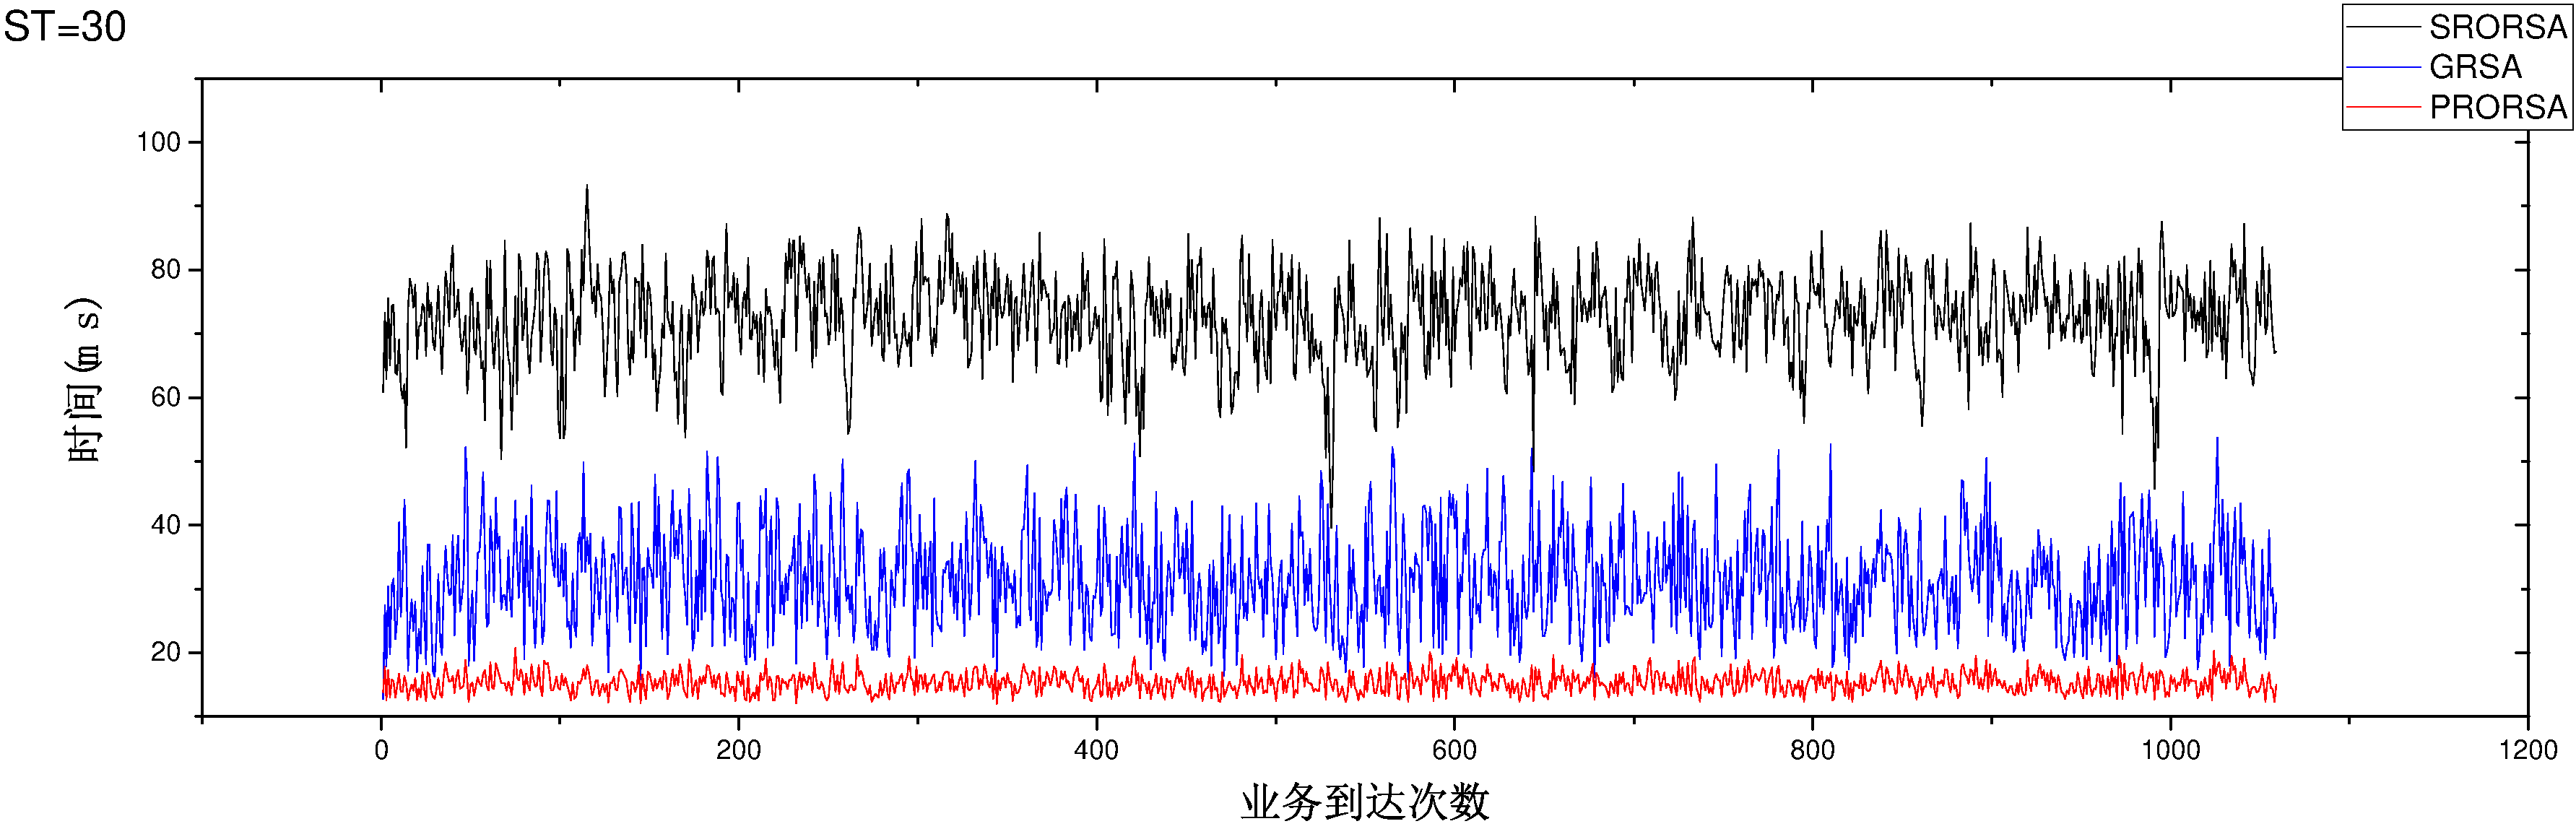
\includegraphics[width=1 \textwidth]{figures/B30T.pdf}}
\end{center}
\caption{{\footnotesize{无权图时间对比(ST=30)}}}
\label{B30T}
\end{figure*}
\begin{figure*}
\setlength{\belowcaptionskip}{-0.5cm}
\begin{center}
{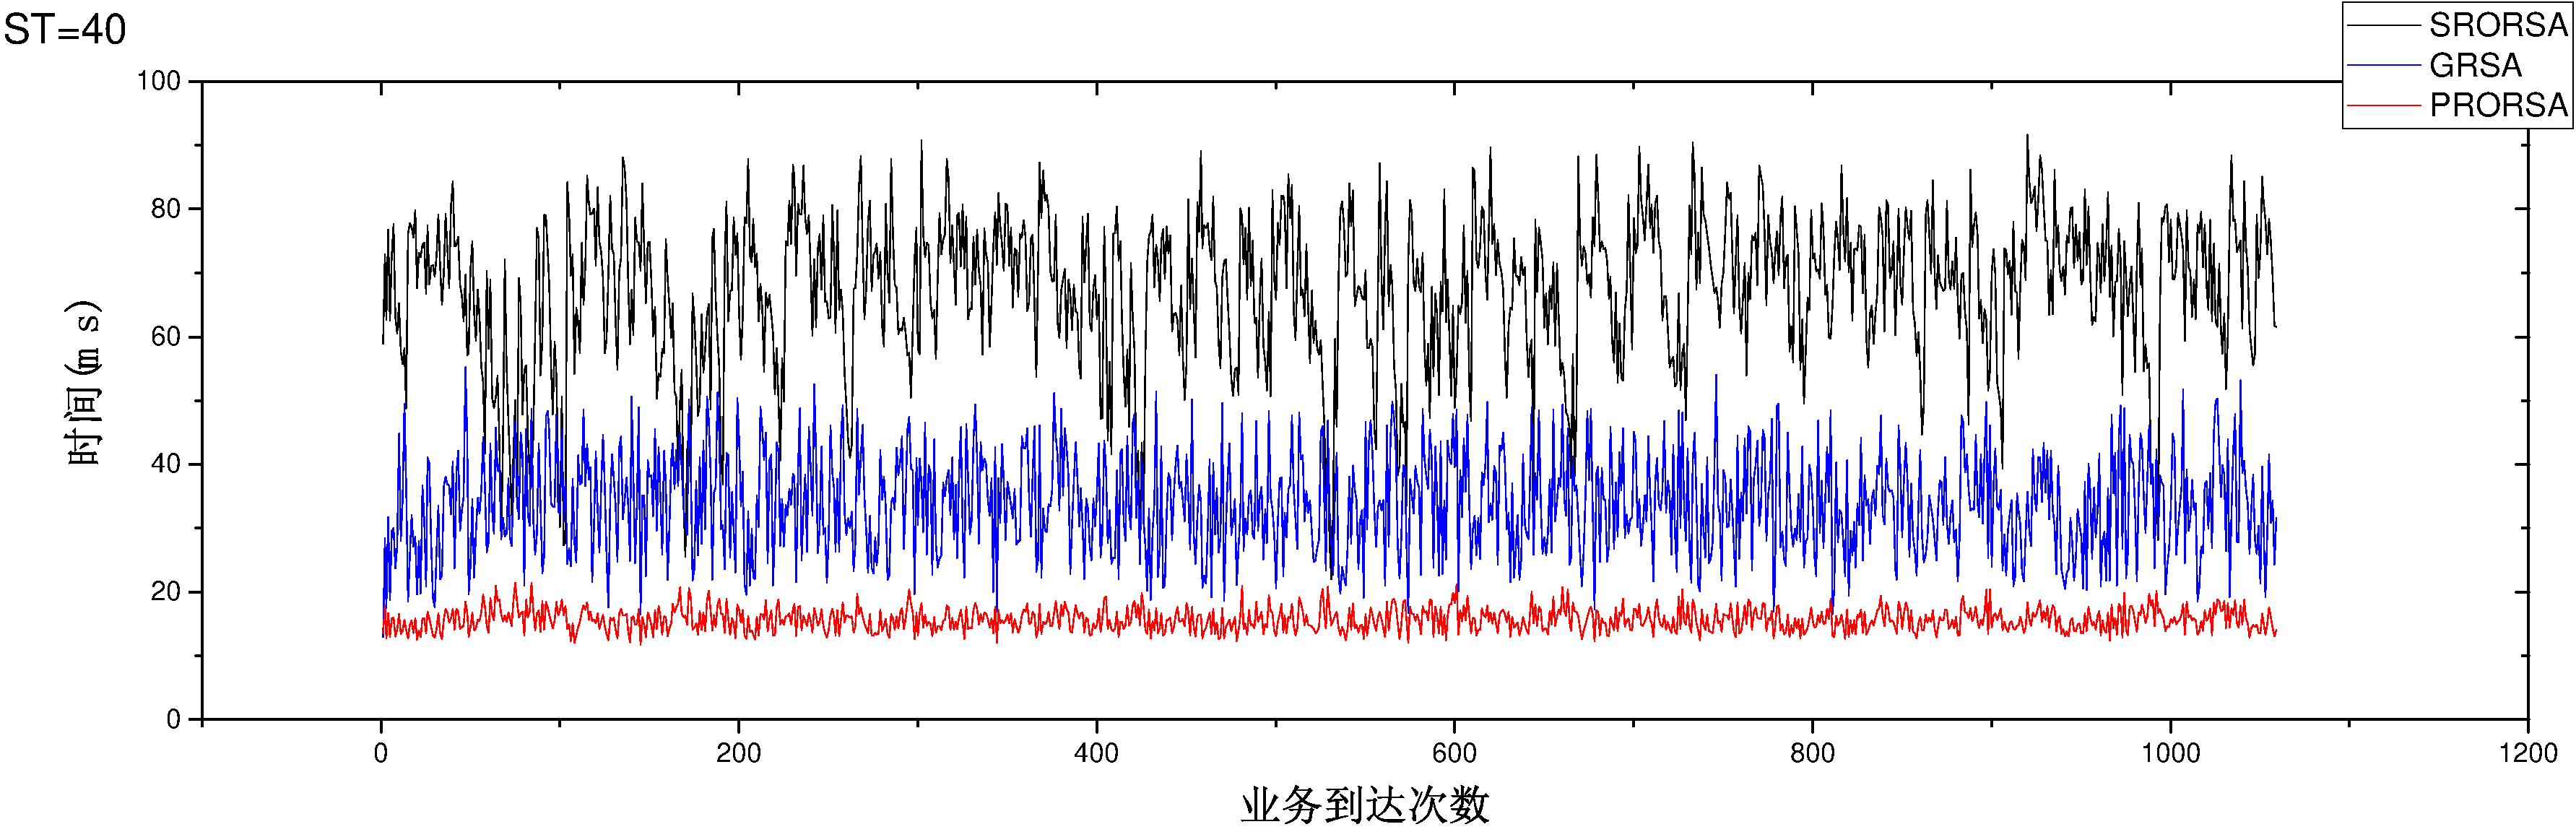
\includegraphics[width=1 \textwidth]{figures/B40T.pdf}}
\end{center}
\caption{{\footnotesize{无权图时间对比(ST=40)}}}
\label{B40T}
\end{figure*}
\subsubsection{阻塞率分析}

图 \ref{B10Z}到图 \ref{B40Z}展示了随着$ST$的变化,PRORSA,SRORSA和GRSA的阻塞率变化情况,其中PRORSA,SRORSA由于是同一种算法,所以其阻塞率几乎一样。当$ST=10$时,我们发现PRORSA/SRORSA的阻塞次数明显小于GRSA。 当$ST=20$时,PRORSA/SRORSA的阻塞次数和阻塞幅度均小于GRSA,在GRSA中出现了一次相对较大的阻塞,但是PRORSA/SRORSA 中没有出现这种不平稳的阻塞率突变。当$ST=30$时,我们发现PRORSA/SRORSA的阻塞次数和阻塞幅度比GRSA小很多,GRSA的平均阻塞率是PRORSA/SRORSA的6倍左右。当$ST=40$时,PRORSA,SRORSA和GRSA的阻塞率都增加很多,但是PRORSA/SRORSA的阻塞情况还是大大优于GRSA,可见在大服务压力的网络中,PRORSA/SRORSA依然能够有效的减小阻塞率。
\begin{figure*}
\setlength{\belowcaptionskip}{-0.5cm}
\begin{center}
{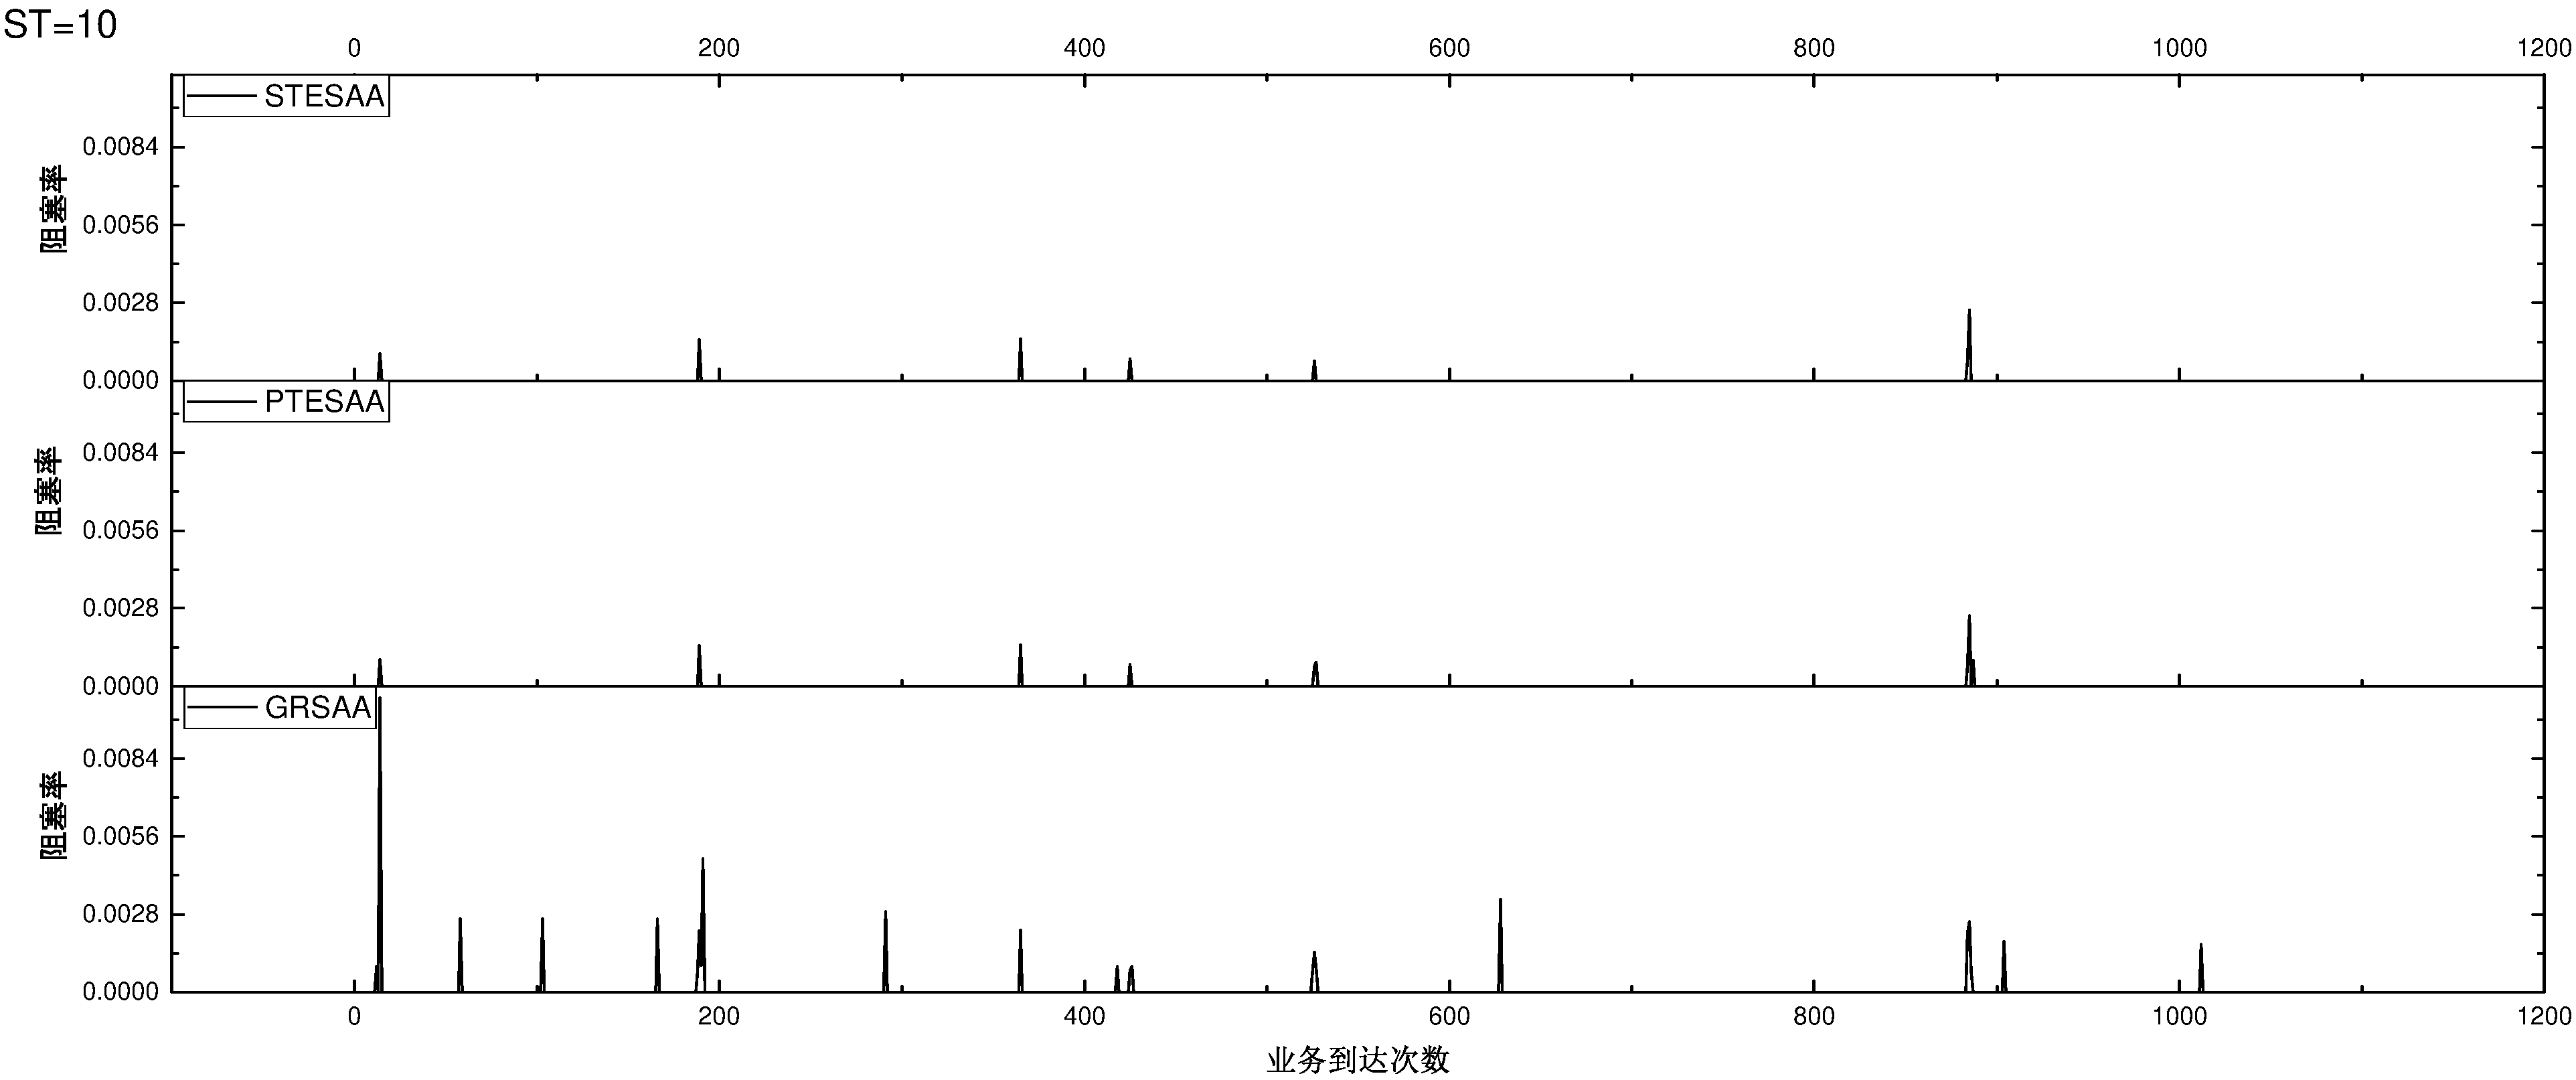
\includegraphics[width=1 \textwidth]{figures/B10Z.pdf}}
\end{center}
\caption{{\footnotesize{无权图阻塞率对比(ST=10)}}}
\label{B10Z}
\end{figure*}
\begin{figure*}
\setlength{\belowcaptionskip}{-0.5cm}
\begin{center}
{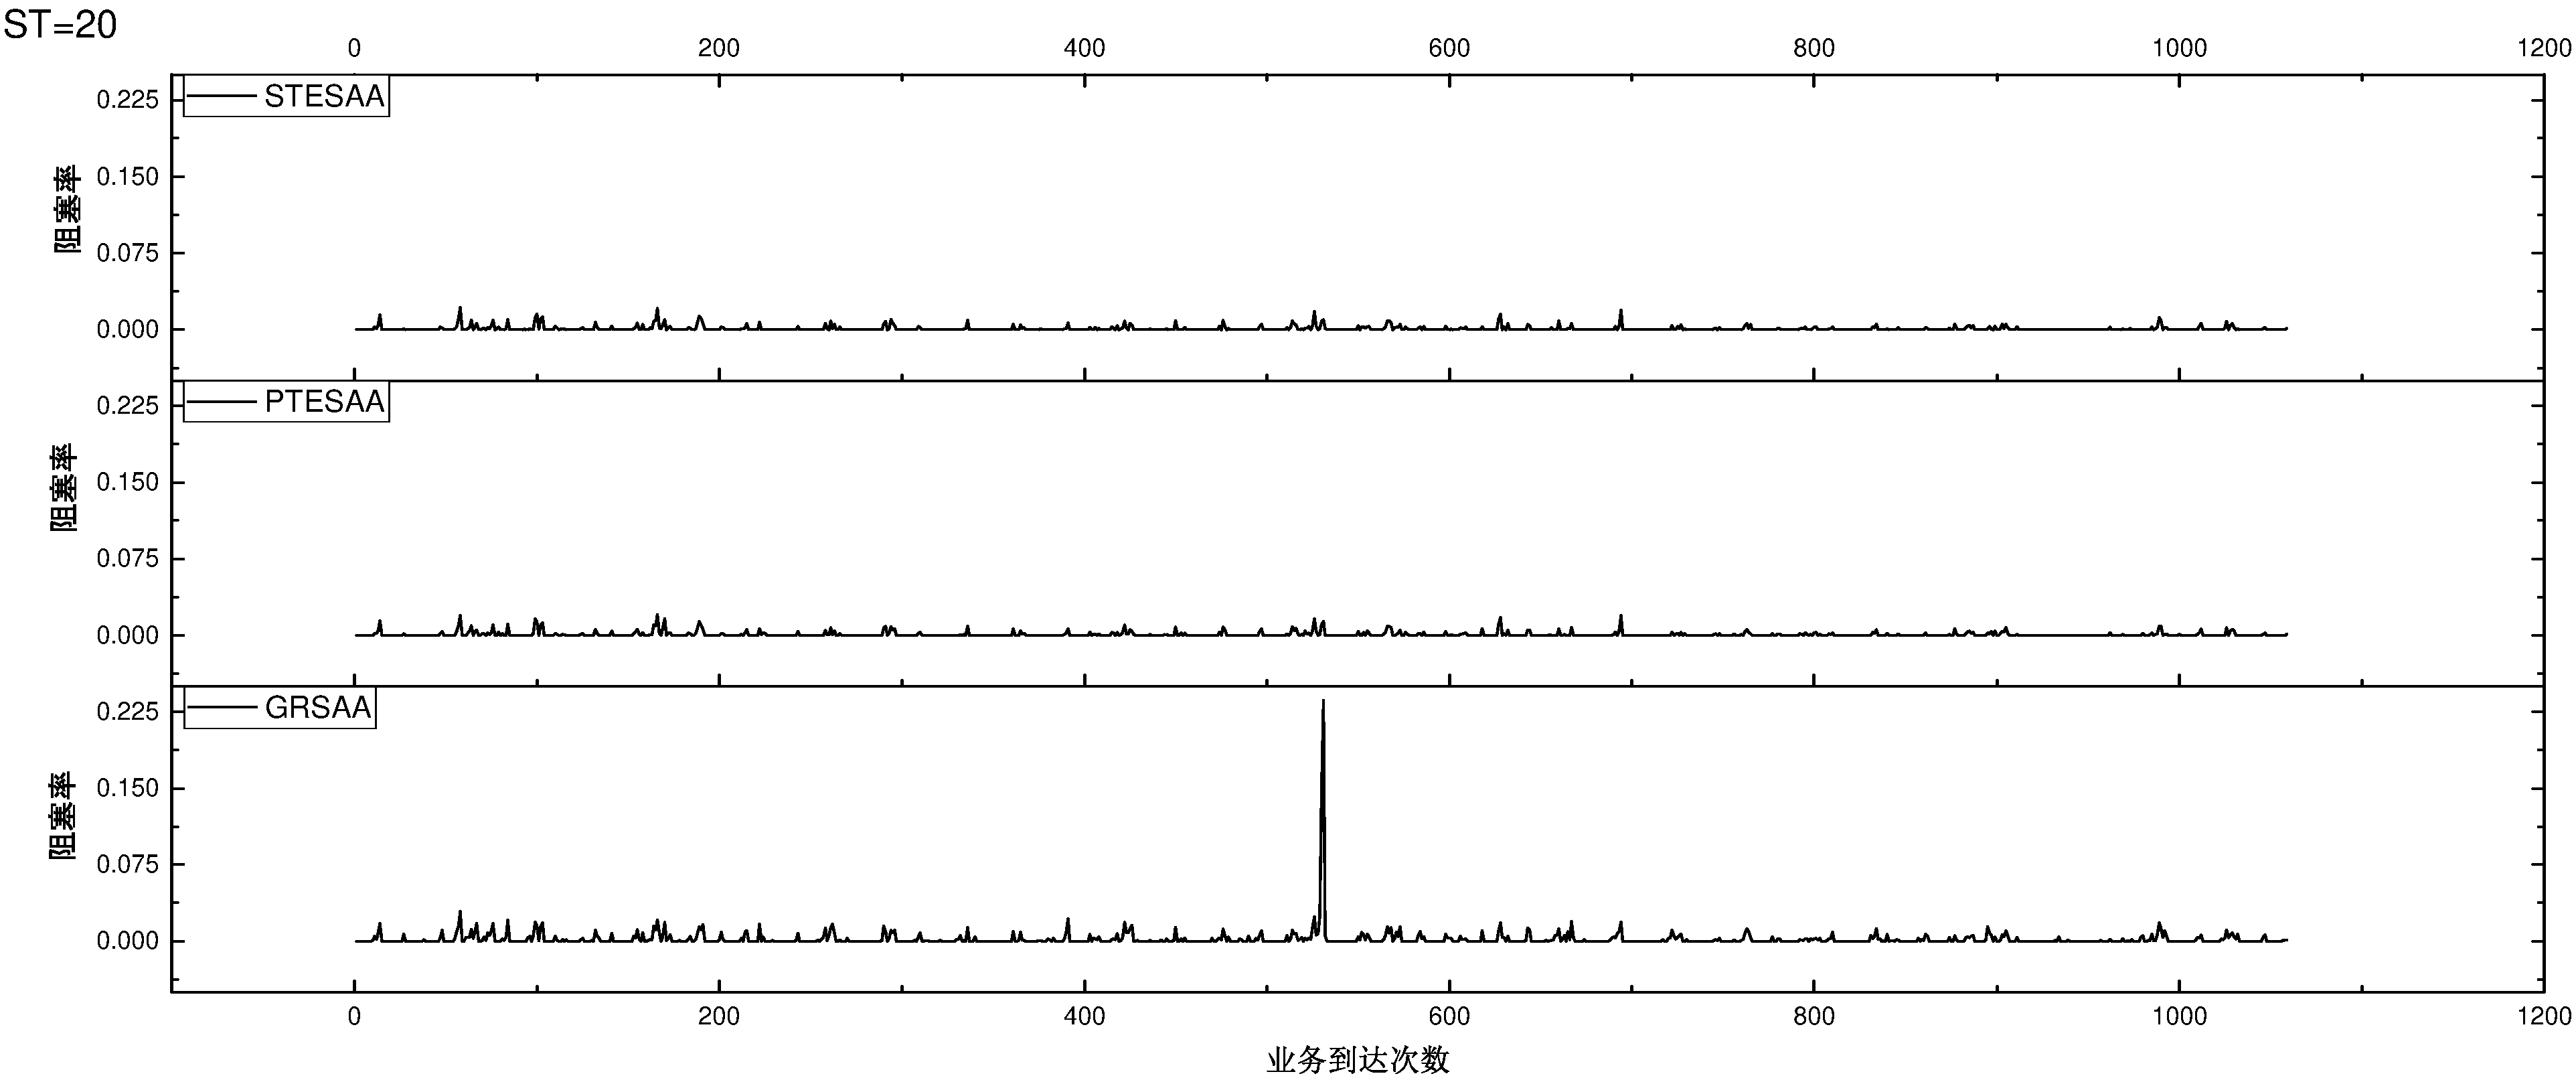
\includegraphics[width=1 \textwidth]{figures/B20Z.pdf}}
\end{center}
\caption{{\footnotesize{无权图阻塞率对比(ST=20)}}}
\label{B20Z}
\end{figure*}
\begin{figure*}
\setlength{\belowcaptionskip}{-0.5cm}
\begin{center}
{\includegraphics[width=1 \textwidth]{figures/B30Z.pdf}}
\end{center}
\caption{{\footnotesize{无权图阻塞率对比(ST=30)}}}
\label{B30Z}
\end{figure*}
\begin{figure*}
\setlength{\belowcaptionskip}{-0.5cm}
\begin{center}
{\includegraphics[width=1 \textwidth]{figures/B40Z.pdf}}
\end{center}
\caption{{\footnotesize{无权图阻塞率对比(ST=40)}}}
\label{B40Z}
\end{figure*}
\subsection{带权图下的仿真结果}
\subsubsection{路径优化分析}
\begin{figure*}
\setlength{\belowcaptionskip}{-0.5cm}
\begin{center}
{\includegraphics[width=1 \textwidth]{figures/H5C.pdf}}
\end{center}
\caption{{\footnotesize{带权图路径权值对比(ST=5)}}}
\label{H5C}
\end{figure*}
\begin{figure*}
\setlength{\belowcaptionskip}{-0.5cm}
\begin{center}
{\includegraphics[width=1 \textwidth]{figures/H10C.pdf}}
\end{center}
\caption{{\footnotesize{带权图路径权值对比(ST=10)}}}
\label{H10C}
\end{figure*}
\begin{figure*}
\setlength{\belowcaptionskip}{-0.5cm}
\begin{center}
{\includegraphics[width=1 \textwidth]{figures/H20C.pdf}}
\end{center}
\caption{{\footnotesize{带权图路径权值对比(ST=20)}}}
\label{H20C}
\end{figure*}
\begin{figure*}
\setlength{\belowcaptionskip}{-0.5cm}
\begin{center}
{\includegraphics[width=1 \textwidth]{figures/H30C.pdf}}
\end{center}
\caption{{\footnotesize{带权图路径权值对比(ST=30)}}}
\label{H30C}
\end{figure*}
\begin{figure*}
\setlength{\belowcaptionskip}{-0.5cm}
\begin{center}
{\includegraphics[width=1 \textwidth]{figures/H40C.pdf}}
\end{center}
\caption{{\footnotesize{带权图路径权值对比(ST=40)}}}
\label{H40C}
\end{figure*}

图 \ref{H5C}到图 \ref{H40C}表示了权值的优化结果,我们把PRORSA和SRORSA的优化结果与贪心算法GRSA的算法权值优化结果进行比较,图中的横坐标表示业务到达的次数,一共产生1051个加入事件,网络链路的权值设置为1到10之间的整数值,当网络状况较好的时候,比如,平均服务时间为$ST=5$ 时,路径权值达到了平均3.5倍的优化,PRORSA和SRORSA 的权值在3-10 之间波动,把业务的路径权值控制在很小的范围,路径优化得非常的理想。另外,随着平均服务时间$ST$ 的增加,贪心算法GRSA的路径平均权值轻微增加,由平均20增加到平均25,这是因为GRSA 是贪心的利用分层图,对链路的权值大小没有限制,不管在拥塞和不拥塞的网络条件下都会产生大量高权值的路径。观察PRORSA 和SRORSA 路径权值随着$ST$ 的变化发现,PRORSA 和SRORSA 的链路权值随着$ST$的增加而不断上涨,从最初的均值为7 到最后($ST=40$) 时的均值为15,这是因为当网络压力较大时,网络中的可用链路会出现匮乏,每个分层图上的路径权值都会很大,使得优化选择的空间变小。
\begin{figure*}
\setlength{\belowcaptionskip}{-0.5cm}
\begin{center}
{\includegraphics[width=1 \textwidth]{figures/H10H.pdf}}
\end{center}
\caption{{\footnotesize{带权图路径跳数对比(ST=10)}}}
\label{H10H}
\end{figure*}
\begin{figure*}
\setlength{\belowcaptionskip}{-0.5cm}
\begin{center}
{\includegraphics[width=1 \textwidth]{figures/H20H.pdf}}
\end{center}
\caption{{\footnotesize{带权图路径跳数对比(ST=20)}}}
\label{H20H}
\end{figure*}
\begin{figure*}
\setlength{\belowcaptionskip}{-0.5cm}
\begin{center}
{\includegraphics[width=1 \textwidth]{figures/H40H.pdf}}
\end{center}
\caption{{\footnotesize{带权图路径跳数对比(ST=40)}}}
\label{H40H}
\end{figure*}

图 \ref{H10H}到 \ref{H40H}显示了带权情况下的路径跳数情况,可以看到当权值优化时,业务的跳数也得到了很大的优化,这是因为权值小的路径常常路跳径较短,而且GRSA是会贪心的在一个分层图上加入业务,导致分层图变得碎片化,容易求得跳数较大的路径,所以即使在带权图的优化中,跳数也会减小很大。
\subsubsection{时间分析}

图 \ref{H5T}到图 \ref{H40T}展示了在不同平均服务时间$ST$下的各种算法的计算时间,当$ST=5$时,我们可以看到通过GPU加速的PRORSA的计算时间是SPROA 的计算时间的1/4,而实际上备选路径部分的GPU加速达到了7-8 倍,但是由于步骤二的快速路径选择过程也需要消耗一部分时间,这部分时间不能进行GPU加速,实际上PRORSA的大部分算法时间花在了步骤二的路径选择上,所以使得总体的加速比下降为4 倍左右。我们发现由于PRORSA的波动幅度比SRORSA的波动幅度小很多,这是因为SRORSA的大部分时间花在计算备选路上,备选路径的计算量随着业务数量和网络链路的占用情况变化较大,而PRORSA的计算量花在步骤二上,计算量变化较小。GRSA的计算时间略高于PRORSA的计算时间,而且GRSA的波动幅度很大,不够平稳,这是因为GRSA贪心策略占用链路资源过多,容易造成分层图链路的碎片化,使得计算量变化较大。
观察到随着$ST$的变化PRORSA的对SRORSA的加速比逐渐下降,这是因为随着网络压力的增加,可用链路变少,使得SRORSA的备选路径计算复杂度下降,PRORSA加速优势变小。另外,随着$ST$的增加,PRORSA 和SRORSA的波动幅度增加,这是因为由于链路繁忙,使得大量业务不能一次性加入,步骤二到步骤一之间的循环次数增加,使得某些业务到达点的业务需要多次的循环,计算时间变长。
\begin{figure*}
\setlength{\belowcaptionskip}{-0.5cm}
\begin{center}
{\includegraphics[width=1 \textwidth]{figures/H5T.pdf}}
\end{center}
\caption{{\footnotesize{带权图时间对比(ST=5)}}}
\label{H5T}
\end{figure*}
\begin{figure*}
\setlength{\belowcaptionskip}{-0.5cm}
\begin{center}
{\includegraphics[width=1 \textwidth]{figures/H10T.pdf}}
\end{center}
\caption{{\footnotesize{带权图时间对比(ST=10)}}}
\label{H10T}
\end{figure*}
\begin{figure*}
\setlength{\belowcaptionskip}{-0.5cm}
\begin{center}
{\includegraphics[width=1 \textwidth]{figures/H20T.pdf}}
\end{center}
\caption{{\footnotesize{带权图时间对比(ST=20)}}}
\label{H20T}
\end{figure*}
\begin{figure*}
\setlength{\belowcaptionskip}{-0.5cm}
\begin{center}
{\includegraphics[width=1 \textwidth]{figures/H30T.pdf}}
\end{center}
\caption{{\footnotesize{带权图时间对比(ST=30)}}}
\label{H30T}
\end{figure*}
\begin{figure*}
\setlength{\belowcaptionskip}{-0.5cm}
\begin{center}
{\includegraphics[width=1 \textwidth]{figures/H40T.pdf}}
\end{center}
\caption{{\footnotesize{带权图时间对比(ST=40)}}}
\label{H40T}
\end{figure*}
\subsubsection{阻塞率分析}

图 \ref{H10Z}到图 \ref{H40Z}展示了带权情况下随着$ST$的变化,PRORSA,SRORSA和GRSA的阻塞率变化情况,由于带权情况下的跳数也优化得很理想,所以其占用的链路资源也较少,阻塞情况得到改善。当$ST=10$时,我们发现PRORSA/SRORSA 的阻塞次数明显小于GRSA。 当$ST=20$ 时,PRORSA/SRORSA 的阻塞次数和阻塞幅度均小于GRSA,在GRSA中出现了一次相对较大的阻塞,但是PRORSA/SRORSA 中没有出现这种不平稳的阻塞率突变。当$ST=30$ 时,我们发现PRORSA/SRORSA的阻塞次数和阻塞幅度比GRSA小很多,GRSA的平均阻塞率是PRORSA/SRORSA的6倍左右。当$ST=40$时,PRORSA,SRORSA和GRSA 的阻塞率都增加很多,但是PRORSA/SRORSA的阻塞情况还是大大优于GRSA。
\begin{figure*}
\setlength{\belowcaptionskip}{-0.5cm}
\begin{center}
{\includegraphics[width=1 \textwidth]{figures/H10Z.pdf}}
\end{center}
\caption{{\footnotesize{带权图阻塞率对比(ST=10)}}}
\label{H10Z}
\end{figure*}
\begin{figure*}
\setlength{\belowcaptionskip}{-0.5cm}
\begin{center}
{\includegraphics[width=1 \textwidth]{figures/H20Z.pdf}}
\end{center}
\caption{{\footnotesize{带权图阻塞率对比(ST=20)}}}
\label{H20Z}
\end{figure*}
\begin{figure*}
\setlength{\belowcaptionskip}{-0.5cm}
\begin{center}
{\includegraphics[width=1 \textwidth]{figures/H30Z.pdf}}
\end{center}
\caption{{\footnotesize{带权图阻塞率对比(ST=30)}}}
\label{H30Z}
\end{figure*}
\begin{figure*}
\setlength{\belowcaptionskip}{-0.5cm}
\begin{center}
{\includegraphics[width=1 \textwidth]{figures/H40Z.pdf}}
\end{center}
\caption{{\footnotesize{带权图阻塞率对比(ST=40)}}}
\label{H40Z}
\end{figure*}
\section{本章总结}
本章首先讨论了EON中的RSA问题,介绍了分层图模型,针对分层图模型设计了RORSA的算法框架,对框架中路由计算部分进行了并行设计,分别在无权图和带权图两种情况下设计了基于GPU的并行算法,实验发现RORSA能够大大优化路径跳数,路径代价和阻塞率,同时,并行算法PRORSA能加速达到5被以上。




\begin{thebibliography}{1}
\bibitem{OpenFlow}
OpenFlow Switch Specification, https://www.opennetworking.org/images\newline/stories/downloads/sdn-resources/onf-specifications/openflow/openflow-switch-v1.5.0.noipr.pdf
\bibitem{SDN}
N. McKeown, T. Anderson, H. Balakrishnan, G. Parulkar, L. Peterson, J. Rexford, S. Shenker, and J. Turner. Openflow: enabling innovation in campus networks. \emph{SIGCOMM Computer Communicaiton Review}, vol. 38, no. 2, pp. 69-74, 2008.
\bibitem{SDN2}
N. McKeown. Software-defined networking[J]. \emph{INFOCOM keynote talk},vol. 17, no. 2,pp. 30-32,2009
\bibitem{SDN3}
Kim H,Feamster N. Improving network management with software defined networking. \emph{IEEE Communications Magazine},vol. 51, no. 2,pp. 114-119,2013
\bibitem{SDNSurvey1}
B. A. Nunes, M. Mendonca, X. Nguyen, K. Obraczka, and T. Turletti,  A survey of software-defined networking :past, present, and future of programming networks, \emph{IEEE Communications Surveys \& Tutorials}, vol. 16, no. 3, pp. 1617-1634, 2014.
\bibitem{SDNSurvey2}
R. Masoudi and A. Ghaffari, Software defined networks: a survey, Journal of Network and Computer Applications, vol.67, pp. 1-25, 2016.


\bibitem{Microsoft}
C.-Y. Hong, S. Kandula, R. Mahajan, M. Zhang, V. Gill, M. Nanduri, and R. Wattenhofer. Achieving high utilization with software-driven wan, \emph{in Proceedings of the ACM SIGCOMM}, pp. 15-26, 2013.
\bibitem{Google}
S. Jain, A. Kumar, S. Mandal, J. Ong, L. Poutievski, A. Singh, S. Venkata, J. Wanderer, J. Zhou, and M. Zhu et al. B4: Experience with a globally-deployed software defined wan, \emph{in Proceedings of the ACM SIGCOMM}, pp. 3-14, 2013.

\bibitem{application}
Cisco Visual Networking Index: Forecast and Methodology, 2016�C2021, http://www.cisco.com/c/en/us/solutions/collateral/service-provider/visual-networking-index-vni/complete-white-paper-c11-481360.html
\bibitem{5G}
S. S. Soliman and B. Song, Fifth generation (5G) cellular and the network for tomorrow, Journal of Network and Computer Applications, vol.85, pp. 84-93, 2017.
\bibitem{DCN}
C. Guo, L. Yuan, D. Xiang, et al. Pingmesh: a large-scale system for data center network latency measurement and analysis, \emph{ACM SIGCOMM}, 2015.
\bibitem{Secondrouting}
S. Gay, R. Hartert, and S. Vissicchio. Expect the unexpected:sub-second optimization ofr segment routing, \emph{IEEE INFOCOM}, 2017.
\bibitem{CUDA}
Nvidia. Programming guide: CUDA toolkit documentation, http://docs.nvidia.com/cuda/cuda-c-programming-guide/index.html\#axzz4mVqP2TEC

\bibitem{CUDAR}
Jason Sanders,Edward Kandrot.GPU高性能之CUDA 实战[M],\emph{机械工业出版社},2011.

\bibitem{ParaTE1}
B. McCormick, F. Kelly, P. Plante, P. Gunning, and P. Ashwood-Smith. Real time alpha-fairness based traffic engineering, \emph{in Procedings of HotSDN}, 2014.
\bibitem{ParaTE2}
K. Kikuta, E. Oki, N. Yamanaka, N. Togawa, and H. Nakazato. Effective parallel algorithm for GPGPU-accelerated explicit routing optimization, \emph{in Procedings of GLOBECOM}, 2015.
\bibitem{TEDef}
Y. Lee and B. Mukherjee. Traffic engineering in next-generation optical networks, \emph{IEEE Communications Surveys \& Tutorials}, vol. 6, no. 3, pp. 16-33, 2004.

\bibitem{TESurvey1}
A. Mendiola, J. Astorga, E. Jacob, and M. Higuero. A survey on the contributions of software-defined networking to traffic engineering, \emph{IEEE Communications Surveys \& Tutorials}, vol. 19, no. 2, pp. 918-953, 2017.
\bibitem{TESurvey}
N. Wang, K. Ho, G. Pavlou, and M. Howarth. An overview of routing optimization for Internet traffic engineering, \emph{IEEE Communications Surveys \& Tutorials}, vol. 10, no. 1, pp. 36-56, 2008.
\bibitem{NP}
Y. Wang and Z. Wang. Explicit routing algorithms for Internet traffic engineering, \emph{in Procedings of International Conference on Computer Communications and Networks}, 1999.

\bibitem{multi-commodity}
M. Pioro and D. Medhi. Routing, flow, and capacity design in communication and computer networks, Morgan Kaufmann Publishers, 2004.
\bibitem{SDNTE}
S. Agarwal, M. Kodialam, and T. V. Lakshman. Traffic engineering in software defined networks, \emph{in proceedings of INFOCOMM}, 2013.
\bibitem{Time}
J. Rexford. Route optimization in IP networks, \emph{in Handbook of Optimizationin Telecommunications}, Springer Science + Business Media, February 2006.

\bibitem{mate}
A. Elwalid, C. Jin, S. Low, and I. Widjaja. MATE: MPLS adaptive traffic engineering, \emph{in proceedings of INFOCOMM}, 2001.

\bibitem{DATE}
J. He, M. Chiang, and J. Rexford. DATE: distibuted adaptive traffic engineering, \emph{in proceedings of INFOCOMM}, 2006.

\bibitem{GPUdeve}
A. R. Brodtkorb, T. R. Hagen, C. Schulz, and G. Halse. GPU Computing in Discrete Optimization Part I: Introduction to the GPU, \emph{EURO Journal on Transportation and Logistics}, vol.2, No. 1, pp. 129-157, 2013.

\bibitem{TSP}
K. Rocki and R. Suda. Accelerating 2-opt and 3-opt local search using GPU in the travelling salesman problem, \emph{In Proceedings of IEEE/ACM International Conference on High Performance Computing
and Simulation (HPCS)}, pp. 489-495, 2012.
\bibitem{VRP}
C. Schulz. Efficient local search on the GPU - investigations on the vehicle routing problem, \emph{Journal of Parallel and Distributed Computing}, Vol. 73, no. 1, 14-31, 2013.

\bibitem{SSP1}
P. Harish and P. J. Narayanan, Accelerating large graph algorithms on the GPU using CUDA. \emph{In Proceedings of International Conference on High performance Computing}, pp. 197-208, 2007.
\bibitem{SSP2}
Q. N. Tran. Designing efficient many-core parallel algorithms for all-pairs shortest-poaths using CUDA. \emph{In Proceedings of International Conference on Information Technology: New Generations}, pp.7-12. 2010.
\bibitem{MST}
S. Rostrup, S. Srivastava, K. Singhal. Fast and memory-efficient minimum spanning tree on the GPU. \emph{In Proceedings of International Workshop on GPUs and Scientific Applications}, 20011.


\bibitem{MLU1}
S. Kandula, D. Katabi, B. Davie, and A. Charny. Walking the tightrope: responsive yet stable traffic engineering, \emph{in Procedings of ACM SIGCOMM}, pp. 253-264, 2005.
\bibitem{MLU2}
H. Wang, H. Xie, and L. Qiu. COPE: traffic engineering in dynamic networks, \emph{in Procedings of ACM SIGCOMM}, pp. 99-110, 2006.
\bibitem{Convex1}
B. Fortz and M. Thorup. Internet traffic engineering by optimizing OSPF weights, \emph{in Procedings of IEEE INFOCOM}, pp. 519-528. 2000.
\bibitem{Convex2}
 D. Xu, M. Chiang, and J. Rexford. Link-state routing with hop-by-hop forwarding can achieve optimal traffic engineering, \emph{IEEE/ACM Transactions on Networking}, vol. 19, no. 6, pp.1717-1730, 2011.
\bibitem{BeyondMLU}
A. Sharma, A. Mishra, V. Kumar, and A. Venkataramani. Beyond MLU: an application-centric comparison of traffic engineering schemes, \emph{in Procedings of INFOCOM}, 2011.

\bibitem{NetworkFlow}
R. K. Ahuja, T. L. Magnanti, and J. B. Orlin, Network flows: Theory, Algorithms, and Applications, Prentice Hall, 1993.
\bibitem{ER}
P. Erdos and A. Renyi. On the evolution of random graphs. \emph{Publications of the Mathematical Institute of the Hungarian Academy of
Sciences}, vol. 5, pp. 17-61, 1960.
\bibitem{BA}
R. Albert and A. L. Barabasi. Statistical mechanics of complex networks. \emph{Reviews of Modern Physics}, vol. 74, pp. 47-97, 2002.
\bibitem{CPLEX}
IBM ILOG CPLEX Optimization Studio, https://www.ibm.com/bs-en/marketplace/ibm-ilog-cplex.

\bibitem{EINC}
A. A. M. Saleh and J. M. Simmons,Technology and architecture to enable the explosive growth of the Internet,\emph{IEEE Communication Magazine.},vol .49,no. 1,pp.126-132
\bibitem{ELAB}
L. Zong, G. N. Liu, A. Lord, Y. R. Zhou and T. Ma.40/100/400 Gb/s mixed line rate transmission performance in flexgrid optical networks,\emph{in 2013 Optical Fiber Communication Conference,Anaheim},2013
\bibitem{EDF}
T. Wuth, M. W. Chbat, and V. F. kamalov, Multi-rate(100G/40G/10G) transport over deployed optical networks,\emph{in 2008 Optical Fiber Communication Conference,San Diego},2008.
\bibitem{ETR}
Spectral grids for WDM applications: DWDM frequencygrid,\emph{ITU-T},G.694.1.
\bibitem{ETRP1}
H. Zang, J. P. Jue, B. Mukherjee.A review of routing and wavelength assignment approaches for wavelengthrouted optical WDM networks,\emph{Optical Networks Magazine},vol. 1,pp.47-59,2000.
\bibitem{ETRP2}
R. Ramaswami and K. N. Sivarajan,Routing and wavelength assignment in all-optical networks.\emph{IEEE Transactions on Networking}, vol.3,no. 5,pp.489-500,1995.
\bibitem{ELAYER}
敖发良 ,胡汉武,全光网静态路由选择和波长分配的分层图算法.\emph{光通信研究},vol.3,2003.
\end{thebibliography}
\end{document}

